% This document is designed to conform to the style and layout
% guidelines stipulated in the document "Preparing and Filing the
% Thesis or Dissertation" at
% 
% http://www.gradstudies.ucdavis.edu/students/filing.html
% 
% and in the sample dissertation title page at
% 
% http://www.gradstudies.ucdavis.edu/students/sample_title.html
% 
% ---Tyrrell McAllister
%

% First we define the point size of the text as a variable because 
% we want some other variables to depend upon it.
%
\newcommand{\pointsize}{11pt}

\RequirePackage{rotating} % for sidewaystable to work

\documentclass[oneside, \pointsize]{amsbook}

% Set the margins with the geometry package.  For the top margin,
% we have a half-inch to the header containing the page number.
% The remaining half-inch to the text will be introduced by our
% definitions of \headwidth and \headsep.
%
%%% EDIT: changed so that all margins are 1 inch
\usepackage[
   includehead,
   includefoot,
     left = 1in, 
      top = 1in, 
    right = 1in,
   bottom = 1in
]{geometry}
\usepackage{fancyhdr}
\usepackage{setspace}
\usepackage{calc}
\usepackage[nocompress]{cite} %%% optional
\usepackage[pdfborder={0 0 0}, pdfpagemode=UseNone, pdfstartview=FitH]{hyperref} %%% optional

% Set \headheight and \headsep so that \headheight + \headsep =
% 0.5in.  Thus, the top of the text will be one inch from the top
% of the page.
% 2019 EDIT: Removes headers and restores top margin to 1 in. 2015 settings are commented out, just delete {0in} to restore.
\setlength{\headheight}{0in} %{\pointsize + 2pt}
\setlength{\headsep}{0in} %{0.5in - \headheight} 

% Protrude page number half-inch into right margin so that it is a
% half-inch from the page's edge.
%
\fancyheadoffset[R]{0.5in} 

% The Preliminary Pages are to be numbered with small Roman
% Numerals that are centered at the bottom of the page.
%
\fancypagestyle{prelim}{%    
   \renewcommand{\headrulewidth}{0pt} 
   \fancyhf{}           
   \pagenumbering{roman}    
   \cfoot{\thepage}       
}

% Pages of the main text are to be numbered with arabic numerals
% that are in the upper right corner of the page.
%
% There are a couple additions to the header here that are not 
% stipulated in the dissertation guidelines.
%
%   (1) A headrule is added by setting the command \headrulewidth 
%   to be 0.4pt.
%
%   (2) The command \fancyhead[L]{\rightmark} causes the current
%   section to be indicated in the upper left of the page.  See 
%   documentation for the fancyhdr to control this display.
%
%2019 EDIT: Removes headers and headrule. 2015 settings are commented out, just delete {0pt} to restore.
\fancypagestyle{maintext}{%
   \renewcommand{\headrulewidth}{0pt} %{0.4pt}
   \pagenumbering{arabic}
   \fancyhf{}
   %\fancyhead[L]{\rightmark}
   \cfoot{\thepage}%%%
}

%%% for the first page of Abstract_Only.tex
\fancypagestyle{abstract1}{%
   \renewcommand{\headrulewidth}{0pt} %{0.4pt}
	 \fancyheadoffset[R]{0in}
   \pagenumbering{arabic}
   \fancyhf{}
}

%%% for pages 2+ of Abstract_Only.tex
\fancypagestyle{abstract2}{%
   \renewcommand{\headrulewidth}{0pt} %{0.4pt}
   \fancyheadoffset[R]{0in}
	 \pagenumbering{arabic}
   \fancyhf{}
   \rhead{\thepage}
}

% Number figures, tables, and equations so that the chapter is
% included in the number.  E.g., use Figure 2.3 for the third
% figure in Chapter 2.
%
\numberwithin{figure}{chapter} 
\numberwithin{table}{chapter}
\numberwithin{equation}{chapter}
\numberwithin{section}{chapter}


% Erin added 5.14.2021: to avoid underfull \vbox (badness 10000) errors
% for pages with many figures, don't force the text to stretch to the
% end of the page (default is 'touchbottom' but set this to 'raggedbottom')
\raggedbottom

% Use this file to load additional packages or define macro
% commands that will be used in the dissertation.
%

\usepackage{graphicx}
\usepackage{caption} %%% optional but probably necessary
\usepackage{subcaption} %%% optional but probably necessary

% packages/settings imported from bees paper:

% Use adjustwidth environment to exceed column width (see example table in text)
%\usepackage{changepage}
% Use Unicode characters when possible
\usepackage[utf8x]{inputenc}
% textcomp package and marvosym package for additional characters
\usepackage{textcomp,marvosym}
% cite package, to clean up citations in the main text. Do not remove.
\usepackage{cite}
% Use nameref to cite supporting information files (see Supporting Information section for more info)
\usepackage{nameref,hyperref}
% line numbers
%\usepackage[right]{lineno}
% ligatures disabled; improves typesetting in LaTeX
%\usepackage{microtype}
%\DisableLigatures[f]{encoding = *, family = * }
% color can be used to apply background shading to table cells only

% Bold the ‘Figure #' in the caption and separate it from the title/caption with a period
% Captions will be left justified
%\usepackage[aboveskip=1pt,labelfont=bf,labelsep=period,justification=raggedright,singlelinecheck=off]{caption}

% Use the PLoS provided BiBTeX style
\bibliographystyle{plos2015}
% Remove brackets from numbering in List of References
%\makeatletter
%\renewcommand{\@biblabel}[1]{\quad#1.}
%\makeatother


\usepackage[english]{babel}


% degree symbol
\usepackage{gensymb}

% fractions:
\usepackage{nicefrac}


% use \textcolor{color}{text} for colored text (e.g. highlight to-do areas)
\usepackage{color}
\newcommand{\ec}[1]{{\color{black} #1}}
\newcommand{\edit}[1]{{\color{black} #1}}
\newcommand{\ecec}[1]{{\color{black} #1}}
\newcommand{\ahb}[1]{{\color{black} #1}}
\newcommand{\africanized}{\ahb{\textit{scutellata}-European}}
\newcommand{\hyb}{\ahb{hybrid}}
\newcommand{\anc}{\ahb{ancestry}}
\newcommand{\A}{\ahb{A}}
\newcommand{\scutellata}{\ahb{\textit{scutellata}}} 

\usepackage[colorinlistoftodos]{todonotes}  

% define custom colors (this one is for figure captions)
\definecolor{Gray}{gray}{.25}

\usepackage{amsmath,amssymb}

% math operators
\DeclareMathOperator{\Cov}{Cov}
\DeclareMathOperator{\Var}{Var}
\DeclareMathOperator{\Normal}{Normal}
\DeclareMathOperator{\Beta}{Beta}
\DeclareMathOperator{\MVN}{MVN}
\DeclareMathOperator{\Uniform}{Uniform}
\DeclareMathOperator{\logit}{logit}
\DeclareMathOperator{\logistic}{logistic}

% maize/hilo macros:
\usepackage{xspace}
\newcommand{\mexicana}{\textit{mexicana}\xspace}
\newcommand{\Mexicana}{\textit{Mexicana}\xspace}
\newcommand{\parviglumis}{\textit{parviglumis}\xspace}
\newcommand{\Parviglumis}{\textit{Parviglumis}\xspace}

% for landscape tables
\usepackage{rotating}
% for splitting lines in table columns
\usepackage{makecell}

\hyphenation{genome-wide pre-print}



% label bibliography as 'references'
\addto{\captionsenglish}{\renewcommand{\bibname}{References}}

\usepackage{setspace} % sets spacing for tables
\renewcommand{\arraystretch}{1.2} % increase spacing in tables


%%% use lowercase letters for subcaption labeling
%\captionsetup[subfigure]{labelfont=rm}

\extrafloats{500}

\begin{document}
   \frontmatter

   \pagestyle{prelim}
   
   % Redefine plain page style so that the first pages of chapters
   % have desired page style.
   %
   \fancypagestyle{plain}{%
      \fancyhf{}
      \cfoot{\thepage}
   }%
   \begin{center}
   \null
   %\vfill
   \textbf{%
      Impact of Introgression on Adaptation and Range Expansions
   }%
   \\
   \bigskip
   By \\
   \bigskip
   ERIN WALKER CALFEE \\
   %2020 EDIT: Removed double-spacing btwn name and DISSERTATION   
   %\bigskip
   %A.B. (Brown University) 2011 \\
   %\bigskip
   %2019 EDIT: Removed line for previous degree.
   DISSERTATION \\
   \bigskip
   Submitted in partial satisfaction of the requirements for the
   degree of \\
   \bigskip
   DOCTOR OF PHILOSOPHY \\
   \bigskip
   in \\
   \bigskip
   Population Biology \\
   \bigskip
   in the \\
   \bigskip
   OFFICE OF GRADUATE STUDIES \\
   \bigskip        
   of the \\
   \bigskip
   UNIVERSITY OF CALIFORNIA \\
   \bigskip
   DAVIS \\
   \bigskip
   Approved: \\
   \bigskip
   \bigskip
   \makebox[3in]{\hrulefill} \\
   Graham M. Coop, Chair \\
   \bigskip
   \bigskip
   \makebox[3in]{\hrulefill} \\
   Jeffrey Ross-Ibarra \\
   \bigskip
   \bigskip
   \makebox[3in]{\hrulefill} \\
   Michael Turelli \\
   \bigskip
   Committee in Charge \\
   \bigskip
   2021 \\
   \vfill
\end{center}

   \newpage
	
	 %%% (optional) copyright page <== this page is not numbered!
	 \thispagestyle{empty}
	 \begin{titlepage}
	 \vspace*{50em}
	 \begin{center}
		 \copyright \ Erin W.\ Calfee, 2020.  All rights reserved.  
	 \end{center}
	 \end{titlepage}
	 \newpage
	 \stepcounter{page}
	
	 %%% (optional) dedication page
	 \thispagestyle{plain}
	 \vspace*{10em}
	 \begin{center}
	 	 \textit{To the Coop lab ... may sound science and the best tea always prevail!}\\
	 	 \vspace*{5em}
	 	
\includegraphics[width=.4\textwidth]{cooplablogo2.png}
	  
	 \end{center}
	 \newpage
   
   % Begin Double Spacing
   %
   \doublespacing
   
   \tableofcontents
   %\renewcommand\@seccntformat[1]{} % disable section numbering after table of contents
   \newpage
   
   \begin{center}
   \textbf{Impact of Introgression on Adaptation and Range Expansions} \\
\end{center}

\section*{Abstract}

	Gene flow between diverged populations is often deleterious (e.g. due to genetic incompatibilities or local adaptation),
	but introgression can also be a source of rapid adaptation, especially to novel niches.
	My thesis focuses on the evolutionary outcomes of these opposing selection forces on introgressed ancestry,
	the repeatability of these outcomes across admixed populations,
	and the consequences for species niches.
	I have developed novel population genetics methods to detect selection in admixed populations,
	and applied these methods to disentangle how demography and selection have shaped the evolution
	and range expansions of two very different species: \textit{scutellata}-European hybrid honey bees and highland maize.
	
	For my first dissertation chapter, I conducted a cross-continental comparison of the outcomes of admixture and selection in \textit{scutellata}-European honey bees.
	\textit{Scutellata} honey bees from South Africa were introduced to the Americas in the 1950s, but soon escaped, and through interbreeding with European honey bees,
	formed a highly successful and invasive hybrid population that spread at $\sim$300km/year across the Americas.
	This is a great system to study the adaptive potential and the limitations of admixture in facilitating rapid range expansions,
	with natural replication in North and South America.
	For this research, I collected and sequenced 300+ bees from two nearly 1000 km transects,
	one in California and one in Argentina, to compare ancestry patterns across their genomes.
	I found evidence of convergent selection favoring African \textit{scutellata} honey bee ancestry at a number of loci in the genome in North and South America.
	These loci are strong candidates for contributing to the high fitness and success of \textit{scutellata}-European hybrid honey bees.
	Because these bees are highly defensive, their continued spread is an agricultural and public health concern.
	I found parallel clines in genomewide ancestry between continents at similar latitudes,
	despite much larger dispersal distances to reach California from the origin of the invasion,
	evidence that many loci across the genome are currently preventing spread to temperate zones.
	
	For my second dissertation chapter, I analyzed the outcome of introgression between maize and its wild highland ‘teosinte' relative, \textit{mexicana},
	which may have facilitated maize’s range expansion from the valleys where it was domesticated up to 3000m in the mountains of Mexico.
	Using a novel method that accounts for background patterns of ancestry variance and covariance between populations
	(e.g. due to gene flow or shared drift post-admixture), I found strong evidence for adaptive introgression from \textit{mexicana} into maize,
	especially among the highest elevation populations, consistent with introgression facilitating maize’s colonization of the highlands.
	I also found loci (including a newly identified inversion) where selection maintains steep ancestry clines across elevation.
	I demonstrated evidence of selection against introgression,
	removing \textit{mexicana} ancestry from near domestication genes and lower recombination regions of the genome (due to linked selection).
	One surprising finding is that despite observations of hybrids in the field,
	and opportunities for gene flow from locally adapted \textit{mexicana} that grows side-by-side with contemporary maize,
	I found little evidence for recent locally sourced haplotypes genomewide or at loci with high local introgression.
	Rather, the majority of introgression is from over 1000 generations ago,
	and has subsequently diverged within the maize background and been sorted by selection along an elevational cline and within individual populations.
	This work has broader impacts for understanding the longer term effects of introgression on range expansions and aiding in the discovery of key loci associated with high-elevation adaptations,
	which may be crucial for future breeding of maize, a global staple, under climate change.
	
	Overall, this thesis adds to our knowledge of the role of introgression in range and niche expansions,
	and provides in-depth genomic analyses of selection and admixture in two agriculturally-important species.

   \newpage
   
   \section*{Acknowledgments}
   First, I would like to thank Graham Coop for encouraging me to trust my ideas and find my own path as a scientist. May I grow into being as kind and thoughtful of a mentor and teacher. 

To Coopons past and present, it’s been a great joy and honor to be your peer: Kristin Lee, Doc Edge, Sivan Yair, Matt Osmond, Emily Josephs, Nancy Chen, Vince Buffalo, Katie Ferris, Jeff Groh, Pavitra Muralidhar, Carl Veller, and Jeremy Berg.

I am grateful to many colleagues and friends for supporting my growth as a scientist. Thank you to Jeff Ross-Ibarra for modeling open science and brightening my time at UC Davis with your enthusiasm for Zea evolution, population genetics, and a-maize-ing puns. Thank you to Michael Turelli for treating me like a junior colleague from day one and sharing your love for good science and good wine. Thank you to Annie Schmitt and Chuck Langley for encouraging me to think broadly. To all of the staff in Evolution and Ecology, and especially Sherri Mann, thank you for your kindness and taking care of all the other things so I could focus on my research. 

To all of the CPB students who met my fledgling scientific ideas with perhaps more enthusiasm then they deserved, you are the spark. A special shout-out to my PhD cohort and close friends for your laughter and support along the way: Vicky Morgan, Kelsey Lyberger, Anita To, Yige Luo, Katherine Corn, Mikaela Provost, Caitlin French, Charlotte Pickett, Matt van Avermaete, Hayley Rousek and Debbie Pattison.

Chapter 1 would not have been completed without the generosity of my collaborators: Graham Coop and Santiago Ramirez for believing in my vision for a cross-continent comparative study and welcoming me into their labs; and Marcelo Nicolás Agra and María Alejandra Palacio for helping me realize this vision with honey bee samples from Argentina. Thank you to Daniel Gates, Anne Lorant, M. Taylor Perkins, Graham Coop and Jeff Ross-Ibarra for their advice and help with Chapter 2.

This thesis would not have been completed without the love and support of my family. Thank you to my parents, Kat and Dave, and sister Alexa for all of your encouragement, and my cat Houdini for being at my side the whole way. Lastly, thank you to my husband Joshua Foster for reminding me there are many mountains to climb (including my PhD) and I can summit any of them if I just keep going up.
   
   \mainmatter
   
   \pagestyle{maintext}
   
   % Redefine plain page style so that the first pages of 
   % chapters have desired page style.
   %
   \fancypagestyle{plain}{%
      \renewcommand{\headrulewidth}{0pt}
      \fancyhf{}
      \cfoot{\thepage}%%%
   }%
   
   \chapter{Selection and hybridization shaped the rapid spread of African honey bee ancestry in the Americas}
   %\label{ch:IntroductionLabel}
   \bigskip
%\begin{center}
%\textbf{Authors and affiliations}
%\end{center}
\begin{flushleft}
	% authors go here:
	%\\
	\begin{center}
	Erin Calfee\textsuperscript{1\edit{,2}},
	Marcelo Nicolás Agra\textsuperscript{\edit{3}},
	María Alejandra Palacio\textsuperscript{\edit{3,4}},
	Santiago R. Ramírez\textsuperscript{1\edit{,2}}, and
	Graham Coop\textsuperscript{1\edit{,2}}
	\end{center}

	%\section*{Affiliations}

	\textsuperscript{1} Center for Population Biology, University of California, Davis, United States of America
	\\
	\textsuperscript{2} Department of Evolution and Ecology, University of California, Davis, United States of America
	\\
	\textsuperscript{3} Instituto Nacional de Tecnología Agropecuaria (INTA), Balcarce, Argentina
	\\
	\textsuperscript{4} Facultad de Ciencias Agrarias, Universidad de Mar del Plata, Balcarce, Argentina
	\\
\end{flushleft}

\section*{Abstract}
Recent biological invasions offer ‘natural’ laboratories to understand the genetics and ecology of adaptation, hybridization, and range limits. One of the most impressive and well-documented biological invasions of the 20th century began \ahb{in 1957 when \textit{Apis mellifera scutellata} honey bees swarmed out of managed experimental colonies in Brazil.} \ahb{This newly-imported subspecies, native to southern and eastern Africa, both hybridized with and out-competed previously-introduced European honey bee subspecies. Populations of \africanized\ \hyb\ honey bees rapidly expanded and spread across much of the Americas in less than 50 years.}
We use broad geographic sampling and whole genome sequencing of over 300 bees to map the distribution of \scutellata\ ancestry where the northern and southern invasions have presently stalled, forming replicated hybrid zones \ahb{with European bee populations} in California and Argentina. California is much \ec{farther} from Brazil, yet these hybrid zones occur at very similar latitudes, consistent with the invasion having reached a climate barrier. At these range limits, we observe genome-wide clines for \scutellata\ ancestry, and parallel clines for wing length that span hundreds of kilometers, supporting a smooth transition from climates favoring \africanized\ \hyb\ bees to climates where they cannot survive winter. \ec{We find no large effect loci maintaining exceptionally steep ancestry transitions. Instead, we find most individual loci have concordant ancestry clines across South America, with a build-up of somewhat steeper clines in regions of the genome with low recombination rates, consistent with many loci of small effect contributing to climate-associated fitness trade-offs.} Additionally, we find no substantial reductions in genetic diversity associated with rapid expansions nor complete dropout of \scutellata\ ancestry at any individual loci \ec{on either continent}, which suggests that the competitive fitness advantage of \scutellata\ ancestry at lower latitudes has a \ec{polygenic} basis and that \africanized\ \hyb\ bees maintained large population sizes during their invasion. To test for parallel selection across continents, we develop a null model that accounts for drift in ancestry frequencies during the rapid expansion. We identify several peaks within a larger genomic region where selection has pushed \scutellata\ ancestry to high frequency hundreds of kilometers past the present cline centers in both North and South America and that may underlie high-fitness traits driving the invasion.

\section*{Author Summary}

Crop pollination around the world relies on \ahb{native and introduced} honey bee populations, which vary in their behaviors and climatic ranges. \ahb{\textit{Scutellata}-European hybrid} honey bees (\ahb{also known as ‘Africanized’ honey bees}) have been some of the most \ecec{ecologically} successful; originating in a 1950s experimental breeding program in Brazil, they rapidly came to dominate across most of the Americas. As a recent genetic mixture of \ahb{multiple} imported \ahb{\textit{Apis mellifera} subspecies},
\africanized\ \hyb\ honey bees have a patchwork of ancestry across their genomes, which we leverage to identify loci with an excess of \scutellata\ or European ancestry due to selection. We additionally use the natural replication in this invasion to compare outcomes between North and South America (California and Argentina). We identify several genomic regions with exceptionally high \scutellata\ ancestry across continents and that may underlie favored \africanized\ \hyb\ \ahb{honey} bee traits (e.g.\textit{Varroa} mite resistance). We find evidence that a climatic barrier has dramatically slowed the invasion at similar latitudes on both continents. At the current range limits, \scutellata\ ancestry decreases over hundreds of kilometers, creating many bee populations with intermediate \scutellata\ ancestry proportions that can be used to map the genetic basis of segregating traits (here, wing length) and call into question the biological basis for binary ‘Africanized’ vs. European bee classifications.

% now start line numbers
%\linenumbers

\section*{Introduction}

Diverging lineages often spread back into secondary contact before reproductive isolation is complete, and so can hybridize. In hybrid zones, multiple generations of admixture and backcrossing create a natural experiment in which genetic variation is ‘tested’ in novel ecological and genomic contexts. The mosaic of ancestries in hybrid zones has allowed researchers to uncover the genetic loci associated with reproductive barriers \ec{(e.g. \cite{Teeter:2008ih, Tavares:2018gi, Powell:2020cr})} and to identify rapidly introgressing high-fitness alleles \ec{(e.g. \cite{Hodgson:2014iq, Hufford:2013_crop_wild, Fitzpatrick:2010bm, Bay:2019ep})}. One promising way forward is to compare ancestry patterns across multiple young hybrid zones and test how repeatable the outcome of hybridization is across these evolutionary replicates.

In this study, we use this powerful comparative framework to better understand the genomic basis of fitness and range limits \ahb{of \africanized\ \hyb\ honey bees}, with replicate \ahb{routes of invasion into} North and South America. \ahb{The range of the western honey bee (\textit{Apis mellifera}) has expanded from Africa, Europe, and western Asia \cite{Cridland:2017el} across much of the globe, assisted by colonialism and the ecological diversity of honey bee subspecies \cite{Moritz:2016bz}. While the Americas have many species of native bees and a long cultural history of beekeeping with honey-producing stingless bees (Meliponini), colonists as early as the 1600s imported European honey bee subspecies for their own apiculture and agriculture uses \cite{Crane:1999vz}, setting off the first honey bee invasion of the Americas \cite{Levine:2008bs}.} \ahb{Through a combination of human-assisted migration and swarming, European honey bees spread across the continent and founded feral populations \cite{Crane:1999vz}.} \ahb{Then i}n 1957, \ahb{swarms from a newly-imported honey bee subspecies from southern and eastern Africa, \textit{Apis mellifera scutellata},} escaped from an experimental breeding program in Brazil and rapidly dispersed. Widely successful, \scutellata\ honey bees both out-competed and hybridized with European-ancestry populations, creating a rapidly advancing \africanized\ admixed population that expanded north and south across the Americas at 300-500 km/year \cite{WINSTON:1992vm}.

\ecec{Colonies of \africanized\ hybrids are likely to respond more strongly to disturbances than colonies with European ancestry (measured as number of stings per minute, reduced time to sting, and longer pursuit distances \cite{Stort:1974bt, Collins:1982cd, Hunt:1998th}).} \ecec{The spread of these more defensive bees (sensationalized as ‘killer bees’, see  critiques \cite{Winston:1992td, roell:2020, Tsing:1995wf, Ksiazek:ahb}) have created new challenges for beekeepers and public health \cite{Winston:1992td, Schumacher:1995ku}}

Control efforts have been largely unsuccessful in \ahb{slowing the invasion or} preventing \ahb{the spread of \scutellata\ ancestry} into commercial colonies \cite{WINSTON:1992vm,Winston:1992td}. However, even without intervention, \scutellata\ \anc\ \ahb{is} unlikely to outcompete European \anc\ in the coldest regions of the Americas because \africanized\ \hyb\ \ahb{honey bees from the neotropics have} low overwinter survival in climates where European bees thrive \cite{Woyke:1973tb, Villa:1991bp}. Models based on winter temperatures and the physiological cost of thermo-regulation predict northern range limits \ahb{for the invasion} that vary from the Central Californian Coast \cite{TaylorJr:1984vg, Harrison:2006gk} up to the border with Canada \cite{Southwick:1990cq}. Thus, the expected impact of \scutellata\ \anc\ on agriculture and queen bee production in the United States is still poorly defined. Broad surveys show that \scutellata\ahb{-like} mtDNA and phenotypes are common in northern Argentina and the southern US, and drop off towards more temperate latitudes, indicating that the rapid spread of these traits has dramatically slowed, if not stopped, on both continents \cite{TaylorJr:1984vg, Sheppard:1991ep, Agra:2018ef, Pinto:2005ep, Loper:1999vi, Kono:2015fi, Lin:2018ha}. However, we lack a genome-wide view of the range limits of \scutellata\ ancestry and do not know whether individual high-fitness alleles have already introgressed into higher latitudes.

\ahb{Previous genomic work on the invasion has shown that \africanized\ \hyb\ honey bees are a genetic mixture of three major genetic groups: A from Africa, C from eastern Europe and M from western Europe \cite{Kadri:2016eg,Wallberg:2014ha,Cridland:2018fx,Whitfield:2006eb,Bozek:2018br,Nelson:2017cj}. Historical sources indicate that the A ancestry is from \textit{A. m.} \scutellata\ \cite{Ruttner:Africa, Schneider:2004fe}, while both M and C ancestries are mixtures of multiple subspecies imported from Europe, e.g. \textit{A. m. ligustica} (C), \textit{A. m. carnica} (C), \textit{A. m. mellifera} (M), and  \textit{A. m. iberiensis} (M) \cite{Crane:1999vz}. Many names have been used previously to refer to \textit{scutellata}-European hybrids in the literature, including ‘African honey bees’, ‘African hybrid honey bees’, or ‘Africanized honey bees’, and the ambiguous acronym ‘AHB’, with these names being used to describe bees identified as having \scutellata\  ancestry on the basis of behavior, morphology, mtDNA, or a range of \scutellata\ autosomal ancestry. Given the wide range of \textit{scutellata}-European ancestry that we find in this study, and that \textit{A. m.} \scutellata\ is only one of at least 10 ecologically diverse \textit{Apis mellifera} subspecies native to Africa \cite{Ruttner:Africa}, we will simply use the label \textit{scutellata}-European hybrids for individuals whose autosomal genome is comprised of a mixture of these ancestries.}

While the key genes remain unknown, \africanized\ \hyb\ \ahb{honey bees} diverge from European-ancestry bees on a number of traits that may have given \ahb{them} a selective advantage during the invasion: they have higher reproductive rates (including faster development times, proportionally higher investment in drone production and more frequent swarming to found new colonies \cite{WINSTON:1992vm}), they have higher tolerances to several common pesticides \cite{Danka:1986ex}, and they prove less susceptible to \textit{Varroa} mites, a major parasite \cite{GuzmanNovoa:1999bu, Vandame:2002kx, Guerra:2000eh, Moretto:1999jx, MedinaFlores:2014fh}. Population monitoring studies show that \textit{Varroa} mites are a strong selective force in the wild and that mite infestations in the 1990s likely contributed to the rapid genetic turnover of feral nest sites from European to \africanized\ \hyb\ colonies in Arizona and Texas \cite{Loper:1999vi, Pinto:2005ep, Bozek:2018br}. \ecec{European ancestry may have also contributed to the success of the invasion; a recent study of \africanized\ \hyb\ bees in Brazil revealed some European alleles at exceptionally high frequency}, \ecec{but this work was under-powered to detect high-fitness \ahb{\textit{scutellata}} alleles due to elevated genome-wide \scutellata\ ancestry (84\%) in the Brazilian population \cite{Nelson:2017cj}.}

There are also a number of candidate traits \ahb{that distinguish} \africanized\ \hyb\ \ahb{honey bees from} European bees and plausibly contribute to a climate-based range limit for the invasion. Smaller bodies \cite{Daly:1978hu} and higher metabolic rates \cite{Southwick:1990cq}, for example, could give honey bees \ahb{with high \scutellata\ ancestry} a competitive advantage in the tropics but come at a cost in cooler climates  \cite{Harrison:2006gk}. In addition to physiological traits, heritable behaviors may also contribute to fitness trade-offs: \africanized\ \hyb\ bees \ahb{from Venezuela to Arizona} preferentially forage for protein-rich pollen (vs. nectar), which supports rapid brood production, but risks insufficient honey stores to thermo-regulate over winter \cite{Danka:1987bk, Fewell:2002ct, Harrison:2006gk}.

\ecec{Other traits associated with \scutellata\ ancestry are of central importance to beekeepers, but their role in the invasion is less clear. Stronger colony-defense behaviors have been reported across much of the range of \textit{scutellata}-European hybrid honey bees \cite{Winston:1992td, Schneider:2004fe} (with some local exceptions, see \cite{RiveraMarchand:2012gn, Avalos:2017jb}). The fitness consequence of these behaviors will depend on the costs of both predation and defense. Similarly, more frequent absconding (leaving a nest site to find another) is undesirable in managed apiaries, but may be adaptive in some environments, e.g. to escape predators or local resource shortages \cite{Winston:abscond}. Selection for these traits is likely to vary across the range of \africanized\ \hyb\ honey bees, depending on the natural and human-mediated environment.}

Here we conduct the first comparative study of the \africanized\ \hyb\ honey bee invasion in North and South America. First, we use broad geographic sampling and whole genome sequencing to map the present-day ancestry clines on both continents, and assess the evidence for a climatic barrier preventing the further spread of \scutellata\ \anc. Next, we use genetic diversity within \scutellata\ ancestry to study the shared bottleneck within and amongst populations due to the rapid expansion during the invasion. Finally, we develop a null model that includes recent drift and use this model to test for outlier loci that may underlie high-fitness \africanized\ \hyb\ \ahb{honey bee} traits and climatic barriers.

\section*{Results}

To survey the current geographic distribution of \scutellata\ ancestry in the Americas, we sampled and sequenced freely foraging honey bees across two latitudinal transects, one in California and one in Argentina, formed from the northern and southern routes of invasion out of Brazil (Fig \ref{fig_map}). We generated individual low-coverage whole-genome sequence data for 278 bees, and added to this data set 35 recently published high-coverage bee genomes from 6 additional California populations sampled 3-4 years prior \cite{Cridland:2018fx}. We inferred genome-wide ancestry proportions for each individual using NGSAdmix \cite{Skotte:2013_NGSadmix} assuming a model of 3 mixing populations, which clearly map to the \scutellata\ (A), eastern European (C), and western European (M) reference panels (Figs \ref{fig_map} and \ref{ngsadmix_refACM}). We leveraged the fact that admixed \africanized\ honey bee populations were formed through a recent mixture of \ahb{known genetic groups} to infer the mosaic of \A, C \ahb{and} M ancestry tracts across the genome of each bee. \ec{For each population, we applied a hidden Markov model that jointly infers the maximum likelihood single-pulse approximation for the generations since mixture and posterior probabilities for local ancestry state, based on read counts from low-coverage sequence data} (ancestry\_hmm \cite{CorbettDetig:2017gh}). The average local ancestry estimates within individuals agree closely with the NGSAdmix genome-wide ancestry estimates (Fig \ref{ngsadmix_vs_ancestry_hmm}, Pearson's $r \geq 0.985$), with the HMM estimating slightly higher minor ancestry for low admixture proportions, likely as a result of some miscalled blocks. Time estimates vary by population, with a median of 47.6 generations in the 62 years since the initial dispersal of \ahb{\scutellata\ queen} bees out of São Paulo (see Fig \ref{supp_time_admixture} for all time estimates). In this section, we first focus on the distribution of genome-wide ‘global' ancestry patterns across the two clines, which we will later compare to the variation in local ancestry at individual loci.

%\begin{figure}[ht]
\begin{figure}[p]
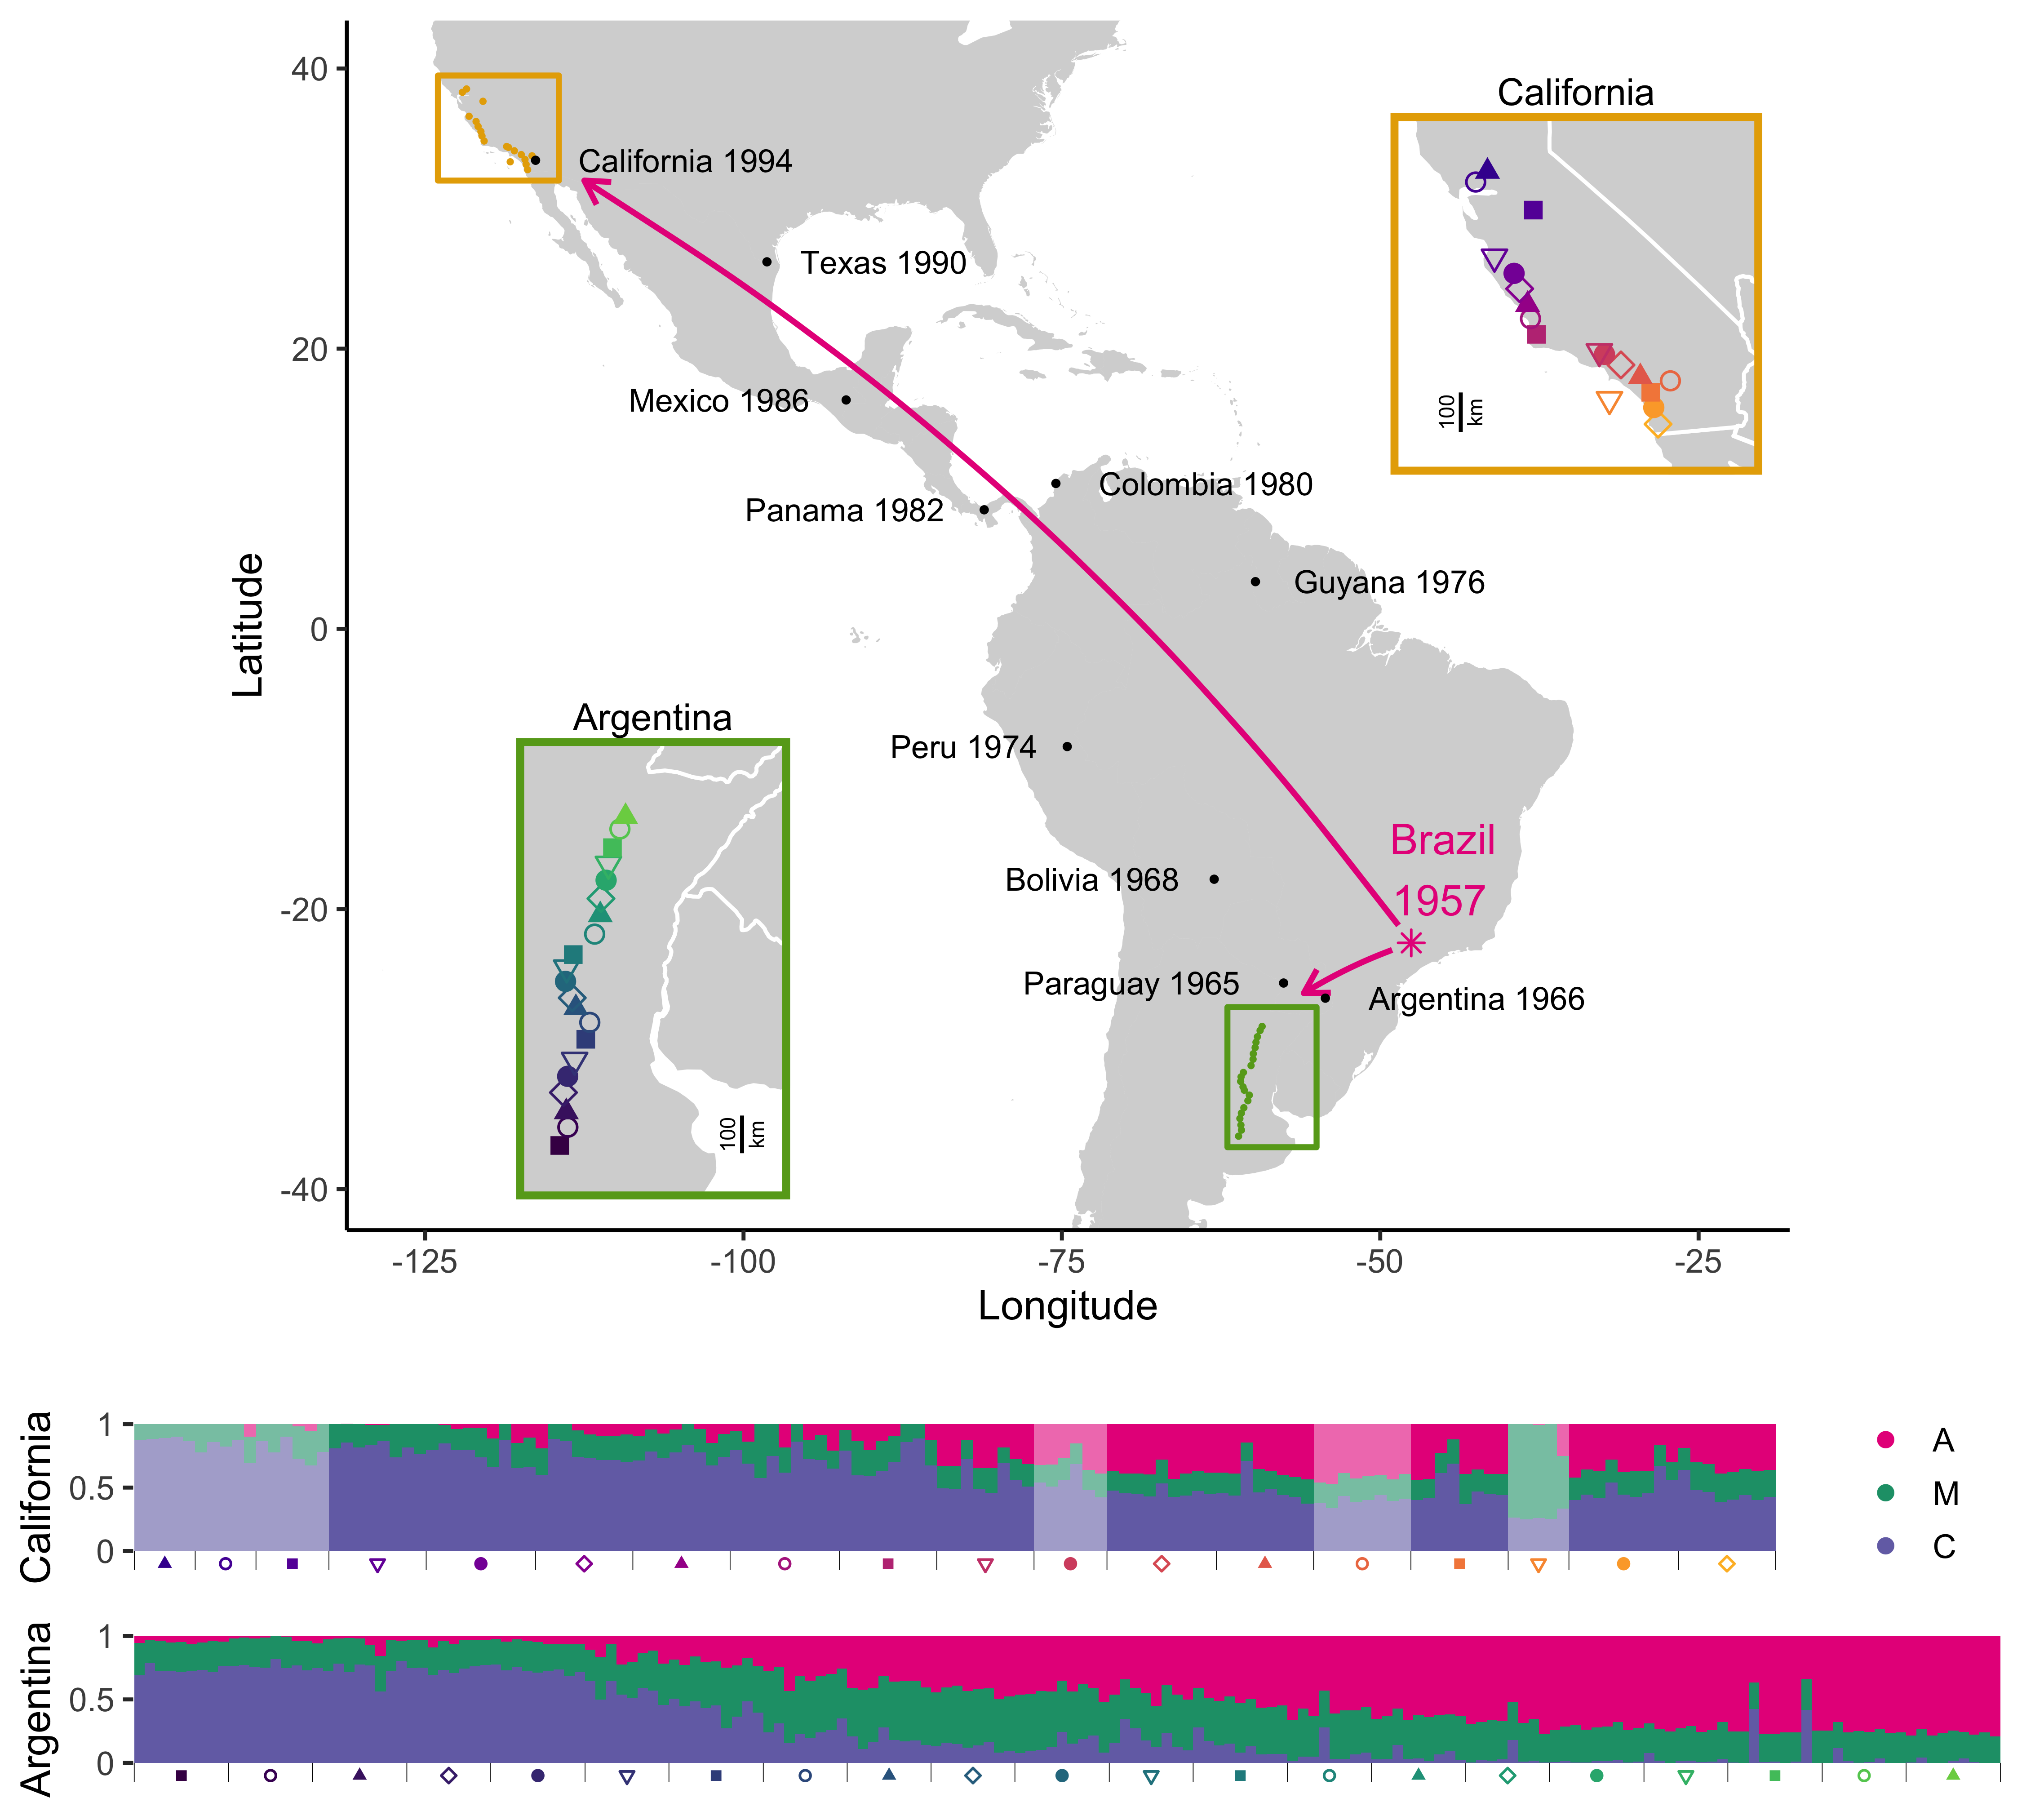
\includegraphics[width=.86\textwidth]{chapter1/figures/world_map_ngsadmix_tall.png}
\caption{ \textbf{\ahb{Spread of \scutellata\ ancestry in the Americas.}} Map of hybrid zones in California and Argentina, with cartoon arrows depicting the two routes of \africanized\ \hyb\ honey bee invasion out of Rio Claro, São Paulo, Brazil. Dates of first occurrence along the routes of invasion are from \cite{WINSTON:1992vm} \cite{Kent:1988il} and \cite{USDA:2009}, with approximate GPS locations extracted from google maps. Insets zoom in on each hybrid zone to show the mean GPS coordinates for each sampled population. \ec{Sampling spanned 646km in California and 878km in Argentina in the north-south direction.} Genome-wide \ahb{\scutellata\ (A), eastern European (C), and western European (M)} ancestry inferred using NGSAdmix for each bee are shown in a bar chart at the bottom, where each vertical bar is one bee and colors indicate proportion ancestry. Populations are arranged by latitude, with samples closest to Brazil on the right. Light fading indicates that a bee comes from the previously published California data set \cite{Cridland:2018fx} and was collected in the field 3-4 years prior to the bees from this study. \ec{These earlier California samples include one island population, Avalon (Catalina Island), indicated by a yellow triangle. Bees from Avalon have majority M ancestry, in contrast to all mainland California bees which have predominantly A and C ancestry. \ec{The underlying maps were created by plotting geographic data from the CIA World DataBank II \cite{world_map} in R \cite{R:2019} using ggplot \cite{R_tidyverse}.}}}
\label{fig_map}
\end{figure}

We observe wide hybrid zones mirrored in North and South America. In Argentina, we find the cline in ancestry spans nearly 900km, from 77\% \scutellata\ \ahb{(A)} ancestry in the north to less than 5\% to the south in Buenos Aires Province. The current geographic range of \A\ \anc\ in South America is broadly consistent with prior studies using a smaller number of genetic markers (e.g. \cite{Sheppard:1991ep, Whitfield:2006eb, Abrahamovich:2015cw, Agra:2018ef}), though the geographic and genetic resolution of these studies is too limited for detailed comparison. In North America, we find that honey bees in California have up to 42\% \A\ ancestry in the south, tapering down to approximately 0\% in Davis, our northernmost sampling site. In comparison, earlier extrapolations based on mitochondrial surveys may have somewhat overestimated genome-wide \A\ ancestry in California (e.g. 65\% of foraging bees in San Diego County \cite{Kono:2015fi} and 17\% in Monterey County \cite{Lin:2018ha} carry \A\ mtDNA haplotypes). We also find excess A-like mtDNA diversity in California. While this finding is potentially consistent with \scutellata\ maternal lines being favored during the expansion into Southern California, this pattern is not strongly replicated in South America and even in North America, \A\ mitochondria do not appear to have introgressed far past the northern range limit for nuclear \A\ ancestry (Fig \ref{mtdna_snps}).

Alongside our genomic cline, we find a corresponding phenotypic cline in worker fore wing size: closer to the equator, sampled bees have increasing \A\ ancestry and shorter wings (Fig \ref{parallel_clines}). By fitting a linear model to predict wing length from genome-wide ancestry, we find that \A\ ancestry can explain a difference of -0.72mm, approximately an 8\% reduction in wing length ($P = 3.65\times10^{-23}, R^2=0.31, n = 269$; see Fig \ref{wing_length_by_A_ancestry}). We tested for a main effect and an interaction term for the South American continent, and found no significant differences in wing length ($P = 0.81$) or its association with ancestry ($P = 0.86$) between the two clines. Thus, in contrast to the rise of dispersal-enhancing traits in other recent invasions (e.g. \cite{Simmons:2015bh, Cwynar:1987, Phillips:2006dc, Hill:1999di}), we see no evidence of a bias for longer wings at larger dispersal distances (California). Genetic crosses have shown that wing length differences between ancestries have a genetic basis \cite{Hunt:1998th} \ec{and} the wing length patterns we observe here are consistent with expectations of an additive polygenic cline based on genome-wide ancestry alone (Fig \ref{parallel_clines}). \ec{However, these phenotypic clines could alternatively be caused purely by developmental plasticity or sorting of within-ancestry genetic variation along a latitudinal gradient. Preliminary evidence that other factors may contribute to the wing length clines observed here comes from a 1991 survey showing that wing length was positively correlated with latitude in California’s feral bee populations before the reported arrival of \africanized\ \hyb\ honey bees \cite{Daly:1991de}. From field-based sampling alone, it remains unclear what portion of the observed phenotypic clines are ancestry-driven}. We performed admixture mapping to test for genetic loci underlying ancestry-associated differences in wing length and did not identify any loci meeting genome-wide significance (Fig \ref{admixture_mapping}).

%\begin{figure}[ht]
\begin{figure}[p]
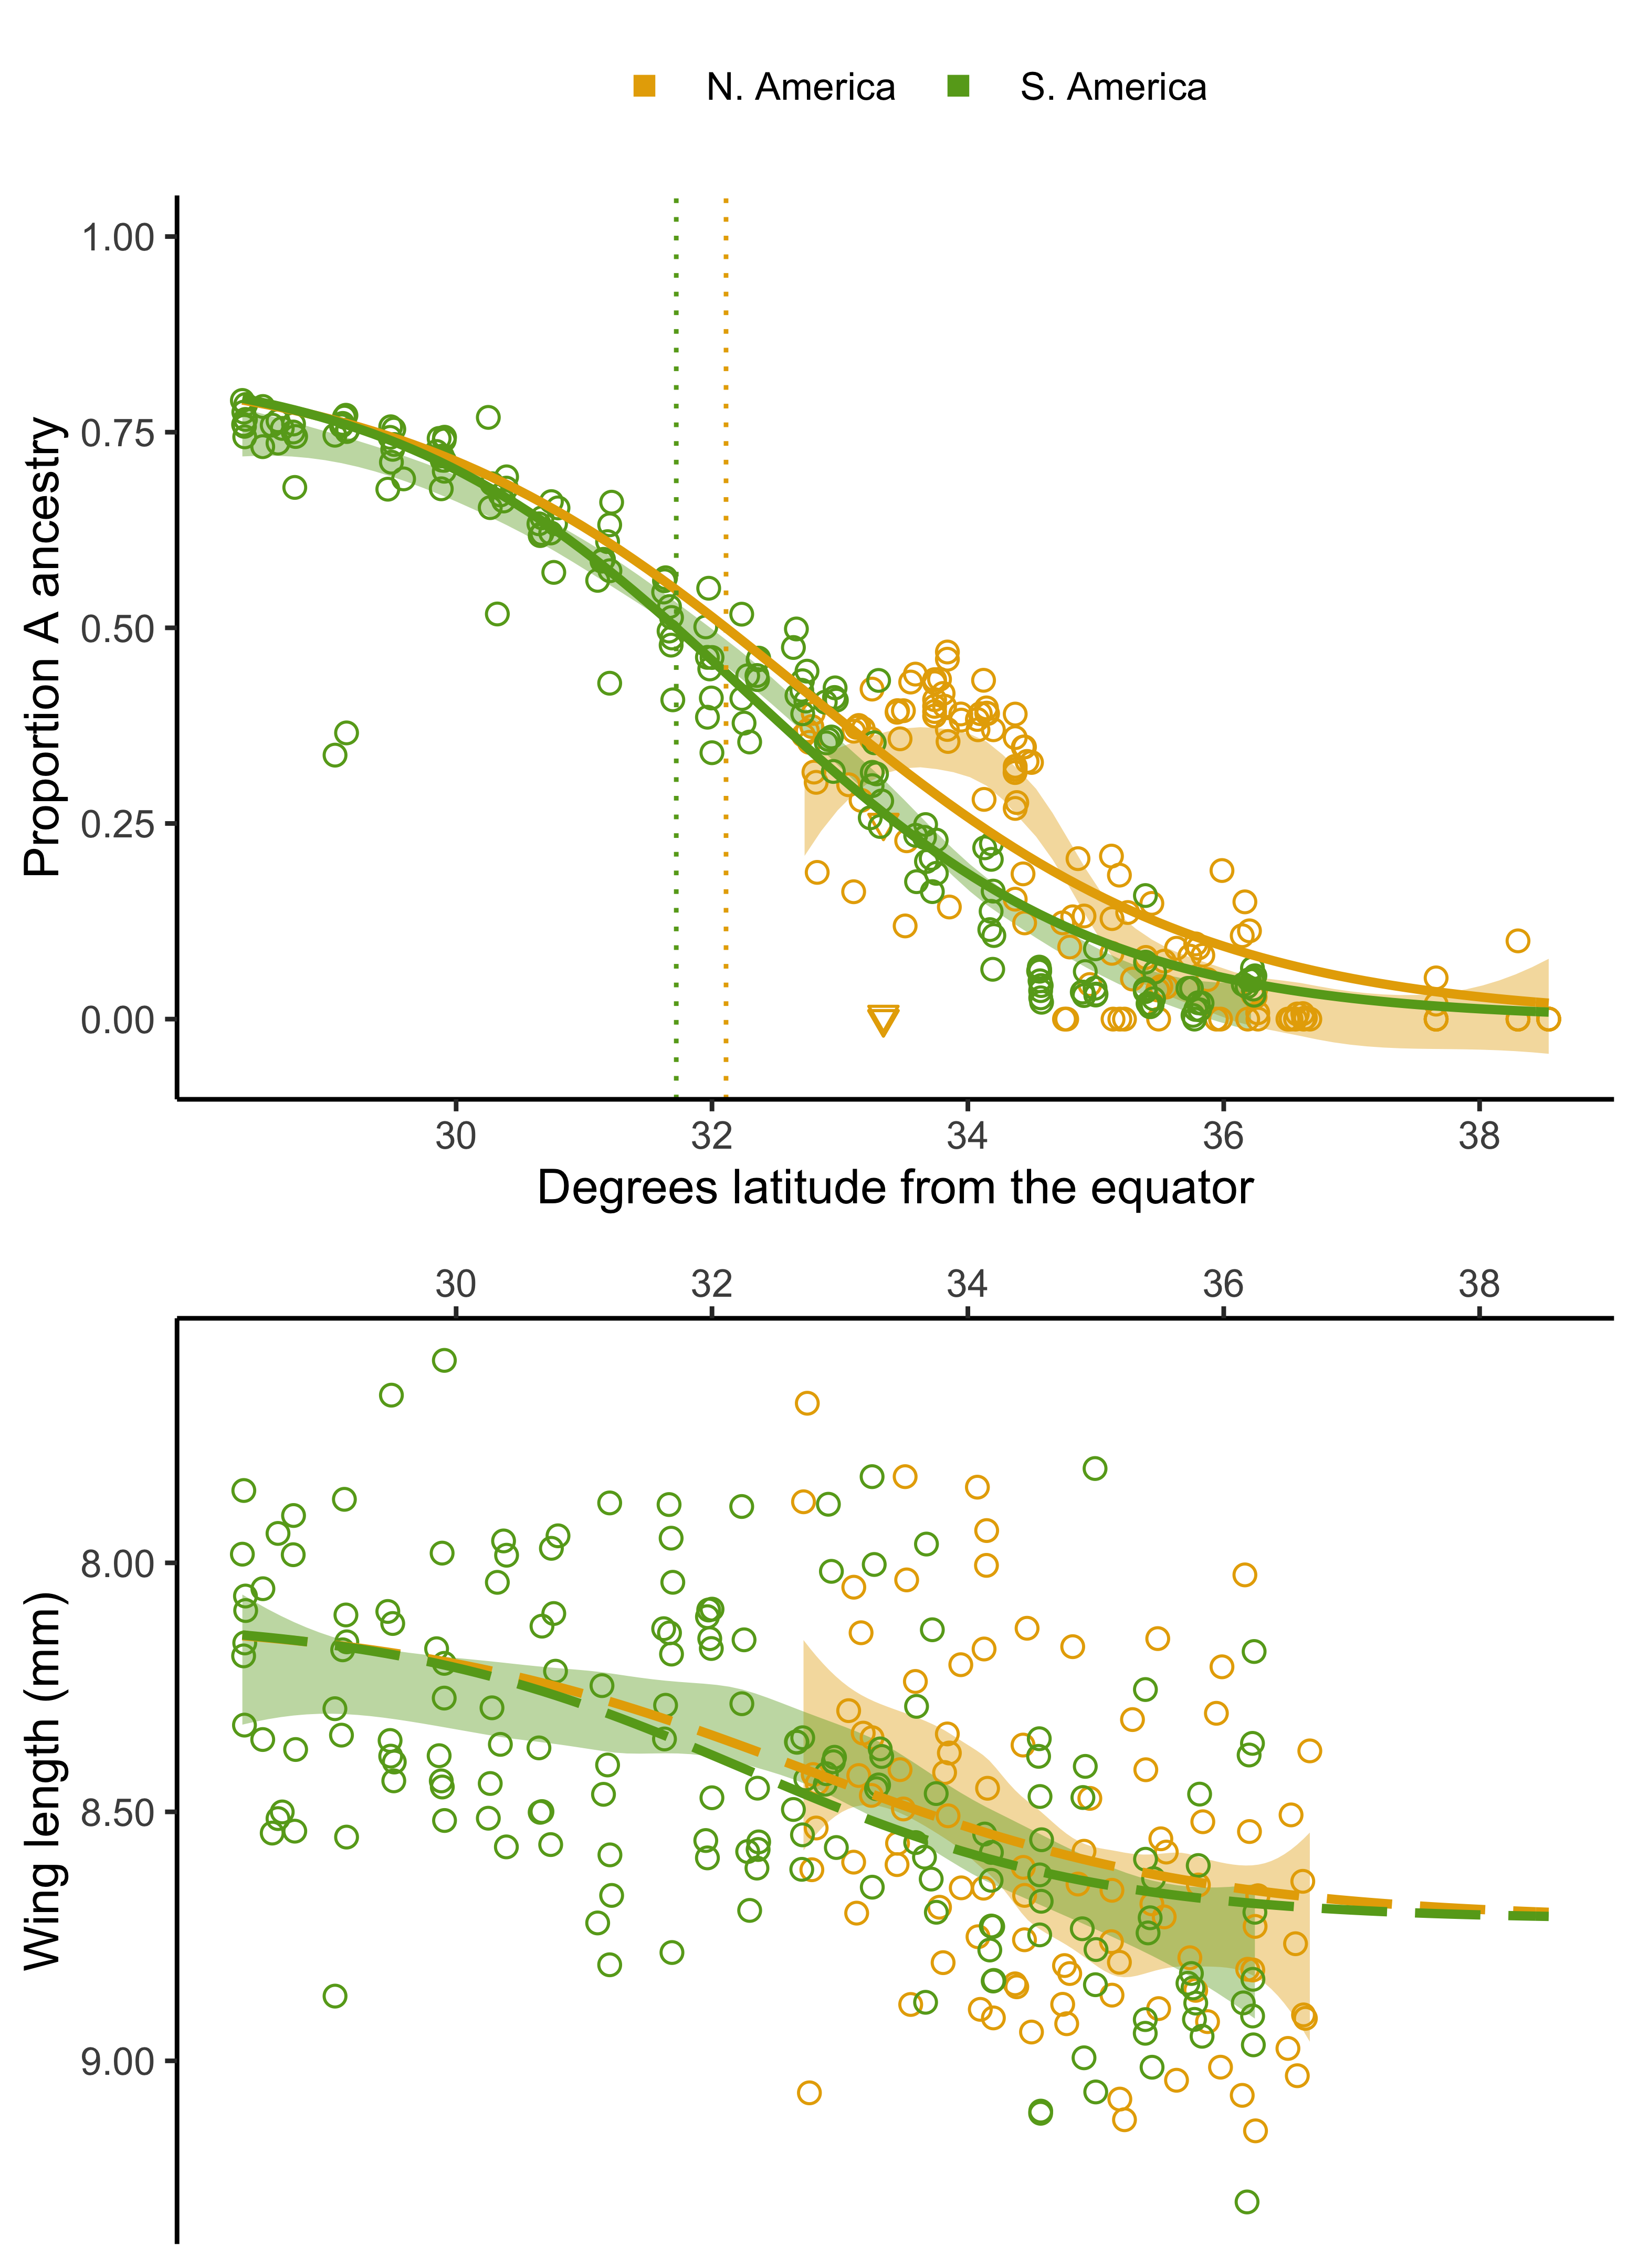
\includegraphics[width = .62\textwidth]{chapter1/figures/A_and_wing_clines.png}
\caption{ \textbf{Clines across latitude.}
Genome-wide ancestry estimates (top) and fore wing lengths (bottom) for individual bees, plotted across absolute latitude and colored by continent. Shading indicates the 95\% confidence intervals for loess curves of the raw data. We also overlay several model-fitted clines: In the top panel, solid curves show the North and South American logistic cline fits for ancestry predicted by latitude, with dotted vertical lines marking the latitude at which bees have predicted 50\% \scutellata\ \ahb{(A)} ancestry, based on these curves. \ec{Samples from Avalon are displayed as orange triangles; Catalina Island has a distinct ancestry composition from mainland California populations and low \A\ ancestry for its latitude.} In the bottom panel, dashed curves show the expected phenotypic cline if wing lengths were fully determined by the clines in ancestry depicted in the top panel. To get these predicted wing lengths, we used the mean ancestry cline as input to the best-fit linear model between ancestry and wing length. Note that the y-axis for wing lengths is reversed (smaller wings are higher) to simplify visual comparisons between the top and bottom panels.}
\label{parallel_clines}
\end{figure}

Our genomic results indicate that the geographic distribution of \scutellata\ \anc\ is presently constrained by climatic barriers, not dispersal. Historical records document an initial rapid spread of \africanized\ \hyb\ honey bees from their point of origin in Rio Claro, São Paulo, Brazil, followed by the formation of seemingly stable hybrid zones at similar latitudes in North and South America. Yet to reach this same latitude, northern-spreading bees had to travel more than five times the distance as southern-spreading \africanized\ \hyb\ honey bee \ahb{populations}.

To more precisely infer the current shape and position of the two hybrid zones, we fit a classic logistic cline model to \ecec{inferred} genome-wide individual \scutellata\ ancestry proportions \cite{Wang:2019ge,Szymura:1986cm,Szymura:1991ia}:

\begin{equation}
\label{eqn:GW_cline}
A_i = \frac{M}{1 + e^{-b(x_i-c)}},
\end{equation}

where $A_i$ is the genome-wide \scutellata\ ancestry proportion inferred for the $i^{th}$ individual bee, $x_i$ is their latitude, $M$ is the asymptotic maximum \scutellata\ ancestry approaching the equator, which is set at 0.84 (i.e. frequency in Brazil \cite{Nelson:2017cj}), $c$ is the cline center, and $w = |\nicefrac{4}{b}|$ is the cline width \ec{(i.e. the inverse of the steepest gradient at the center of the cline)}.

Each degree latitude corresponds to approximately 111km and presents a natural way to compare cline position and shape between the two zones. We fit this model in R using non-linear least squares \ec{(although maximum likelihood or Bayesian estimation are generally preferred when the errors can be fully parameterized, here least squares allows for unknown drift variance in addition to binomial sampling variance)}. We find that the two hybrid zones have strikingly similar positions (Fig \ref{parallel_clines}), with cline centers that differ by less than half a degree (32.72\degree N vs. 32.26\degree S), and no statistically significant difference in cline steepness. To better understand the mechanisms underlying this parallelism between continents, we tested four possible explanatory climate variables to see if we could identify a better predictor for \scutellata\ ancestry across our two zones than latitude: Mean annual temperature (\degree C), mean temperature of the coldest quarter (\degree C), minimum temperature of the coldest month (\degree C), and mean annual precipitation (cm) (downloaded from WorldClim.org \cite{Hijmans:2005ke}). We fit clines for both hybrid zones jointly using these four environmental variables in turn as predictors in Eq \ref{eqn:GW_cline} in place of $x_i$, and compared these results to fits based on absolute latitude and, as a neutral dispersal model, distance from São Paulo.

We find that latitude is the best individual predictor of genome-wide global ancestry, and mean annual temperature the second-best predictor, as assessed by AIC (see \nameref{table_AIC_climate_clines}). While latitude provides the best-fitting cline, we find it unlikely that latitude or daylight per se is the relevant selection gradient. Temperature and precipitation are closely coupled to latitude across our transect in Argentina, so nearly all of our resolution to disentangle latitude from environmental gradients comes from micro-climates within California, and for precipitation, the contrast between continents (Fig \ref{supp_bioclim}). However, we failed to identify specific environmental variables that may be driving the relationship with latitude, either because we did not include the relevant environmental variable(s) or because the climate data does not reflect the selection environment of sampled bees, e.g. due to mismatches in scale or selective habitat use by bees within a foraging range.

Despite limited resolution on the climate variables driving the latitudinal gradient, our comparative framework allows us to firmly reject a neutral model based on distance from the point of introduction in Brazil, because a single dispersal rate cannot generate predictions that simultaneously fit the clines in North and South America well (see \nameref{table_AIC_climate_clines}).

In addition to these global ancestry estimates, we measure variation in local ancestry frequencies across the genome, which are informative about recent evolutionary history. \ahb{\textit{Scutellata}} ancestry frequencies at individual \ec{loci} \ahb{will} vary around their genome-wide mean due to finite sampling, but also evolutionary processes, including drift and selection. If two populations have shared gene flow post-admixture, at \ec{loci} where one population has higher than average \scutellata\ ancestry frequencies, the second population will also tend to have higher than average \scutellata\ ancestry. We capture this genetic signature in an ancestry covariance matrix, where each entry represents how much a pair of populations co-deviate in locus-specific \scutellata\ ancestry away from their individual genome-wide means (Fig \ref{K_matrix}). We expect ancestry co-variances to build up along each route of the \africanized\ \hyb\ honey bee invasion as a result of shared drift post-admixture. Indeed, we do observe positive ancestry covariances for nearby populations within each hybrid zone. We attribute this pattern to shared demographic history, but also note that weak selection for a specific ancestry at many loci genome-wide could also generate these positive covariances. Unexpectedly, we find that populations in more temperate North and South America, i.e. at opposite ends of the expansion, have higher ancestry correlations with each other than with populations situated between them. This robust signal is a general pattern that holds true on average across chromosomes (Fig \ref{fig_mean_k_by_chr}), and so isn't driven by individual outlier loci, and persists across recombination rate bins (Fig \ref{fig_mean_k_by_r}). These similar ancestry patterns in geographically distant populations are potentially consistent with a genome-wide signature of convergent selection to cooler climates or convergent selection by beekeepers at higher latitudes. \ec{Another possible explanation is recent long-distance migration (e.g. international bee exports); however, we investigated genetic covariance patterns within \ahb{A, C, and M} ancestries and found no clear evidence of gene flow between the high-latitude cline endpoints (see methods).}

\begin{figure}[ht]
%\begin{figure}[p]
%\begin{center}
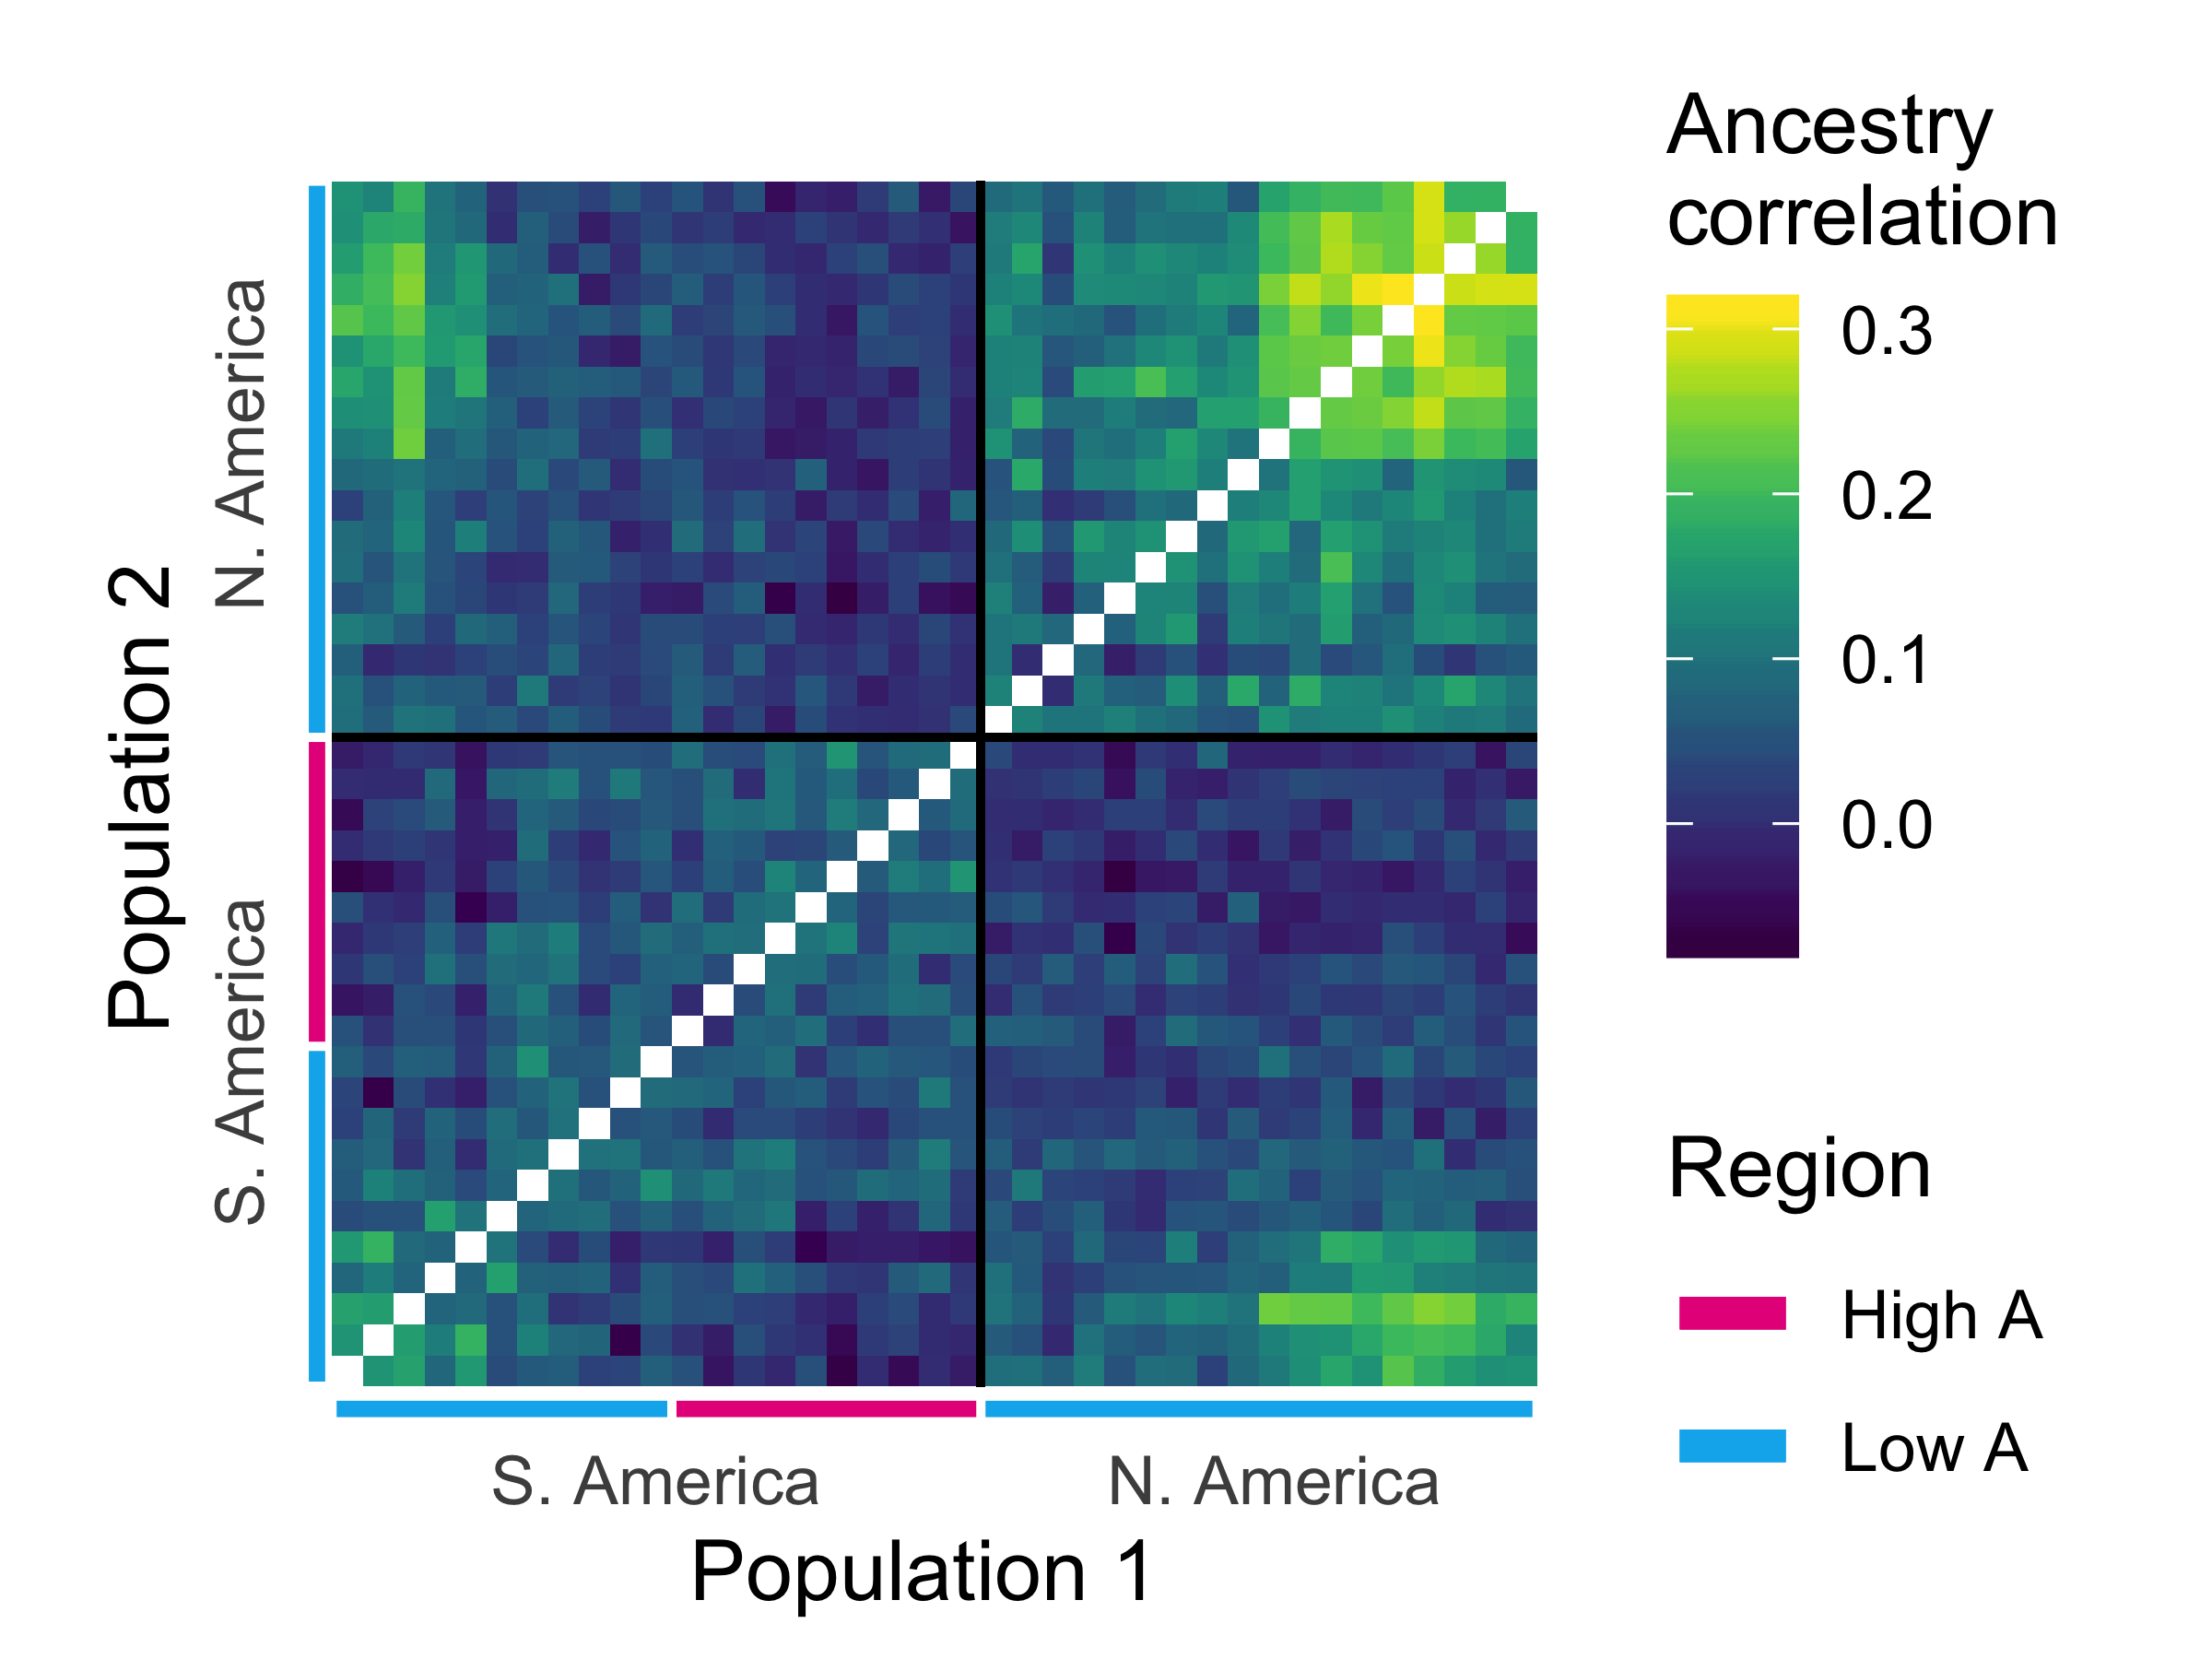
\includegraphics[width = .8\textwidth]{chapter1/figures/k_correlation_matrix_all_pops.png}
%\end{center}
\caption{
\textbf{Correlated ancestry across populations.} Shared drift in ancestry shown as an ancestry correlation matrix (see methods). Populations are ordered by latitude and diagonals are left blank (within-population correlations = 1). \ec{Low and high \A\ ancestry regions of each hybrid zone are defined relative to the estimated latitude of the cline center for genomewide ancestry. About half of the sampled South American populations, and all of the North American populations, fall in the ‘low A' half of their respective hybrid zones.}}
\label{K_matrix}
\end{figure}


\subsection*{Genetic basis of the climate barrier}

To identify loci that may be contributing to a climate barrier, we looked for \ec{loci} with steeper than expected ancestry clines across latitude in South America. We estimated best-fitting logistic ancestry clines \ec{at} $\sim$542k \ec{single nucleotide polymorphisms (SNPs)} across the genome by re-fitting eqn. \ref{eqn:GW_cline}, where $x_i$ is the population latitude and $A_i$ is the population-mean local \scutellata\ ancestry at a focal SNP, and the maximum \scutellata\ ancestry $M$ is 1. \ec{Similar cline models have been fit using likelihood methods under some simplifying assumptions about the form of the errors (e.g. \cite{Szymura:1986cm, Szymura:1991ia}). We instead use non-linear least squares to fit cline parameters without specifying a full error model and then quantify the effects of more complex unmodeled errors (including ancestry variances and covariances) through simulation. We simulated data for 100,000 independent loci undergoing drift, which we used to estimate the expected distribution of neutral clines and calculate false-discovery rates. For each simulated locus, we independently drew a vector of population ancestry frequencies from a multivariate-normal model of drift,} $\text{\A\ ancestry} \sim \MVN(\alpha, K)$, where $\alpha$ is the vector of population mean genome-wide \scutellata\ \ahb{(A)} ancestry proportions, and the $K$ matrix measures the expected variance and covariance in ancestry away from this mean (Fig \ref{K_matrix}), and is empirically calculated using all loci across the genome (see methods for additional details). \ec{We limit the analysis of clines at individual loci to South America where, unlike North America, we have samples spanning both halves of the hybrid zone to inform parameter estimates. While cline analyses can be used to identify both adaptive introgression and barriers to introgression (by analysing cline center displacement in addition to cline steepness \cite{Gompert:2017fl}), here we focus on barrier loci and approach identifying positively selected loci using alternative methods that can be applied to both hybrid zones (see “Scan for ancestry-associated selection”).}

We find no evidence to support a simple genetic basis or environmental threshold to the climate barrier. Ancestry clines in South America are reasonably concordant across most SNPs; 95\% of cline centers fall within a 1.6 degrees latitude range, with a long tail that appears to be due to adaptively introgressing loci (identified as outliers below, see Fig \ref{violin_ind_clines}). We find no strongly selected individual barrier loci that exceed our 5\% false-discovery-threshold for cline steepness, set by MVN simulation of background ancestry patterns. \ec{On average, individual SNP clines in South America are 960km wide (w = 8.65 degrees latitude)}, and the steepest cline in the genome still takes approximately 555km (w = 5 degrees latitude) to fully transition from \scutellata\ to European ancestry. These wide clines, coupled with the evidence for parallel genome-wide clines in North and South America, are consistent with selection tracking smooth climate transitions over broad geographic regions rather than a discrete environmental step. Furthermore, concordance in clines across SNPs in South America suggests that many loci are associated with climate-based fitness trade-offs.
\ec{Under a polygenic climate barrier, we expect locally-adapted loci to be found across the genome but steeper clines to be more commonly maintained in regions with low recombination rates. This is because selected loci create stronger barriers to gene flow when there is tight genetic linkage than when selection acts on each locus independently \cite{Barton:1983fx}.} We test this theoretical prediction in South America and find enrichment for steeper clines in regions of the genome with low recombination. The empirical top 5\% steepest clines in South America are found on all 16 chromosomes and are enriched in regions of the genome with low recombination. Steep clines comprise 12.7\% CI$_{95}$[8.4\%-16.5\%] of loci from the lowest recombination rate quintile vs. only 3.3\% CI$_{95}$[3.0\%-3.6\%] of loci from the highest recombination rate quintile. The average effect of recombination is a 50km decrease in mean cline width between the highest and lowest recombination rate quintiles ($\Delta b = 0.028$, [0.017-0.038]).

\subsection*{Diversity and rapid expansion}
From their point of origin in Brazil, \africanized\ \hyb\ honey bees invaded much of the Americas in less than 50 years \cite{Schneider:2004fe}. Such rapid expansion can lead to high rates of drift in the continually bottle-necked populations at the front of the wave of expansion, i.e. those populations sampled furthest from Brazil. To test this expectation, we calculated nucleotide diversity, $\pi$, for each sampled population (Fig \ref{pi_by_lat}). Despite much further distances traveled to the northern hybrid zone, we do not observe a more pronounced bottleneck in California than in Argentina, suggesting that the expanding wave of \africanized\ \hyb\ honey bees maintained large population sizes (and did not experience strong 'allele surfing' \cite{Excoffier:2009em}).

\begin{figure}[ht]
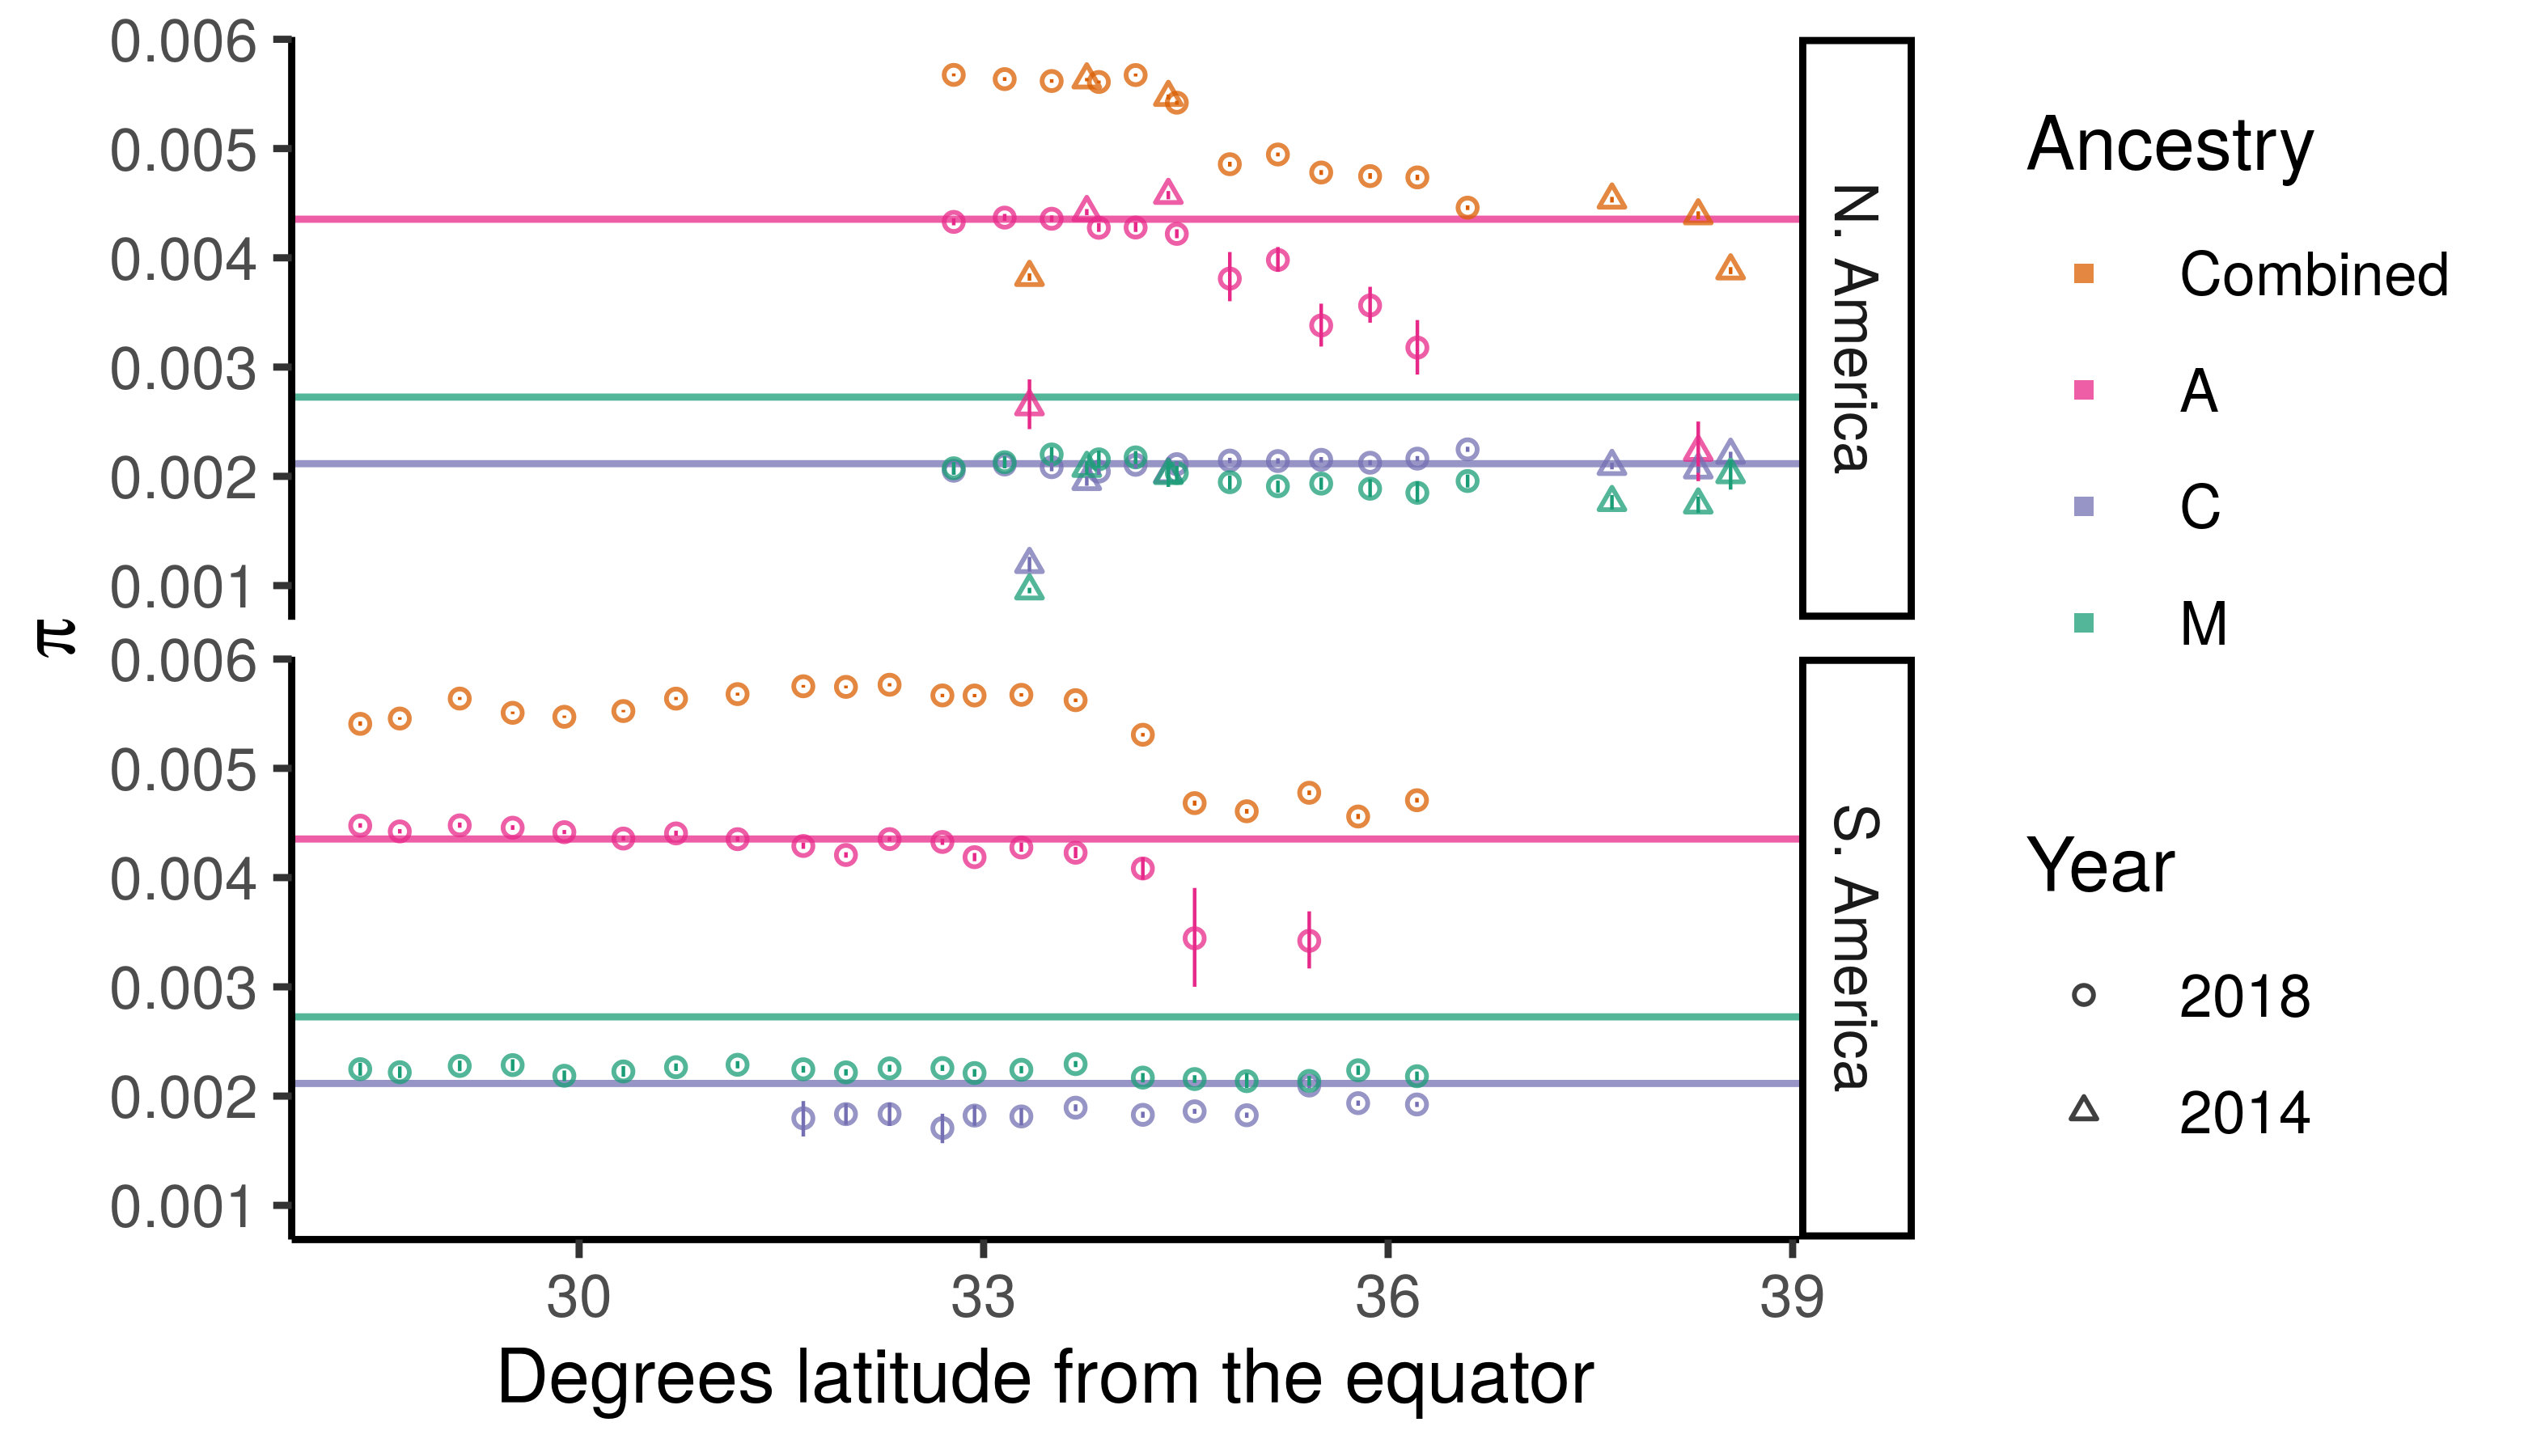
\includegraphics[width=\textwidth]{chapter1/figures/pi_by_latitude.png}
\caption{
 \textbf{Allelic diversity ($\pi$) across the hybrid zones.} For each population, we estimated allelic diversity genome-wide and within high-confidence homozygous ancestry states. Horizontal lines show the genome-wide diversity within the reference panels. Vertical lines show the 95\% confidence interval for each estimate, based on a simple block bootstrap CI using 1cM blocks. For several populations in the tails of the cline, we do not show A and/or C within-ancestry estimates because these populations have too few high-confidence ancestry blocks for accurate estimation (see methods). The low diversity outlier at 33.34 degrees latitude in the N. American cline is the 2014 Avalon sample, which comes from a small island population off the coast of California.}
\label{pi_by_lat}
\end{figure}

\ahb{\textit{Scutellata}-European hybrid} bee populations are consistently more diverse than reference bee populations because they are genetic mixtures of these diverged groups. We do, however, observe a drop in diversity in the tails of both hybrid zones starting at approximately 34.5\degree latitude from the equator. We tested whether this drop in diversity is necessarily the result of a bottleneck or can be explained solely by a cline in mean ancestry composition from more diverse \scutellata\ and highly admixed genomes to less diverse European stock. To test this alternative, we predicted population diversity from a simple weighted average of A, C, and M reference allele frequencies and the observed population ancestry proportions. We find that based on ancestry composition alone, we do expect a drop in diversity across the hybrid zones, although the observed drop is slightly less than our predictions (Fig \ref{pred_vs_obs_pi}).

Levels of diversity within European C and M ancestries are similar to the reference panels and stable across latitude, evidence that a diverse population of European ancestry bees hybridized with \scutellata\ bees as they expanded away from Brazil. We also find high diversity within \A\ haplotypes in both hybrid zones, again consistent with no bottleneck associated with the rapid expansion. However, the diversity in the \A\ ancestry background does decline in populations furthest from the equator, which is consistent with either strong filtering of \scutellata\ haplotypes by selection or stochastic haplotype loss due to small \scutellata-ancestry population sizes in the tails of the clines.

\subsection*{Scan for ancestry-associated selection.}
We identified loci with unusually high \A\ ancestry frequencies, a signal of natural selection, using our MVN simulations of background covariance in ancestry to set a false discovery rate. The ancestry covariances are important to account for when testing for putative selected loci that depart from genome-wide background ancestry patterns, because deviations in ancestry are correlated across populations. Although many population pairs have only small positive ancestry covariances, the cumulative effect on the tails of the distribution of \A\ ancestry frequencies in the larger sample is striking. These covariances can confound outlier tests for selection which only consider variance from sampling (e.g. Poisson-\edit{b}inomial, e.g. \cite{Nelson:2017cj}). We find that by incorporating background patterns of shared drift (or weak genome-wide selection) into our null model, we can match the bulk of the observed ancestry distributions across the genome (Fig \ref{fig_A_CA_AR_density}).

%\begin{figure}[ht]
\begin{figure}[p]
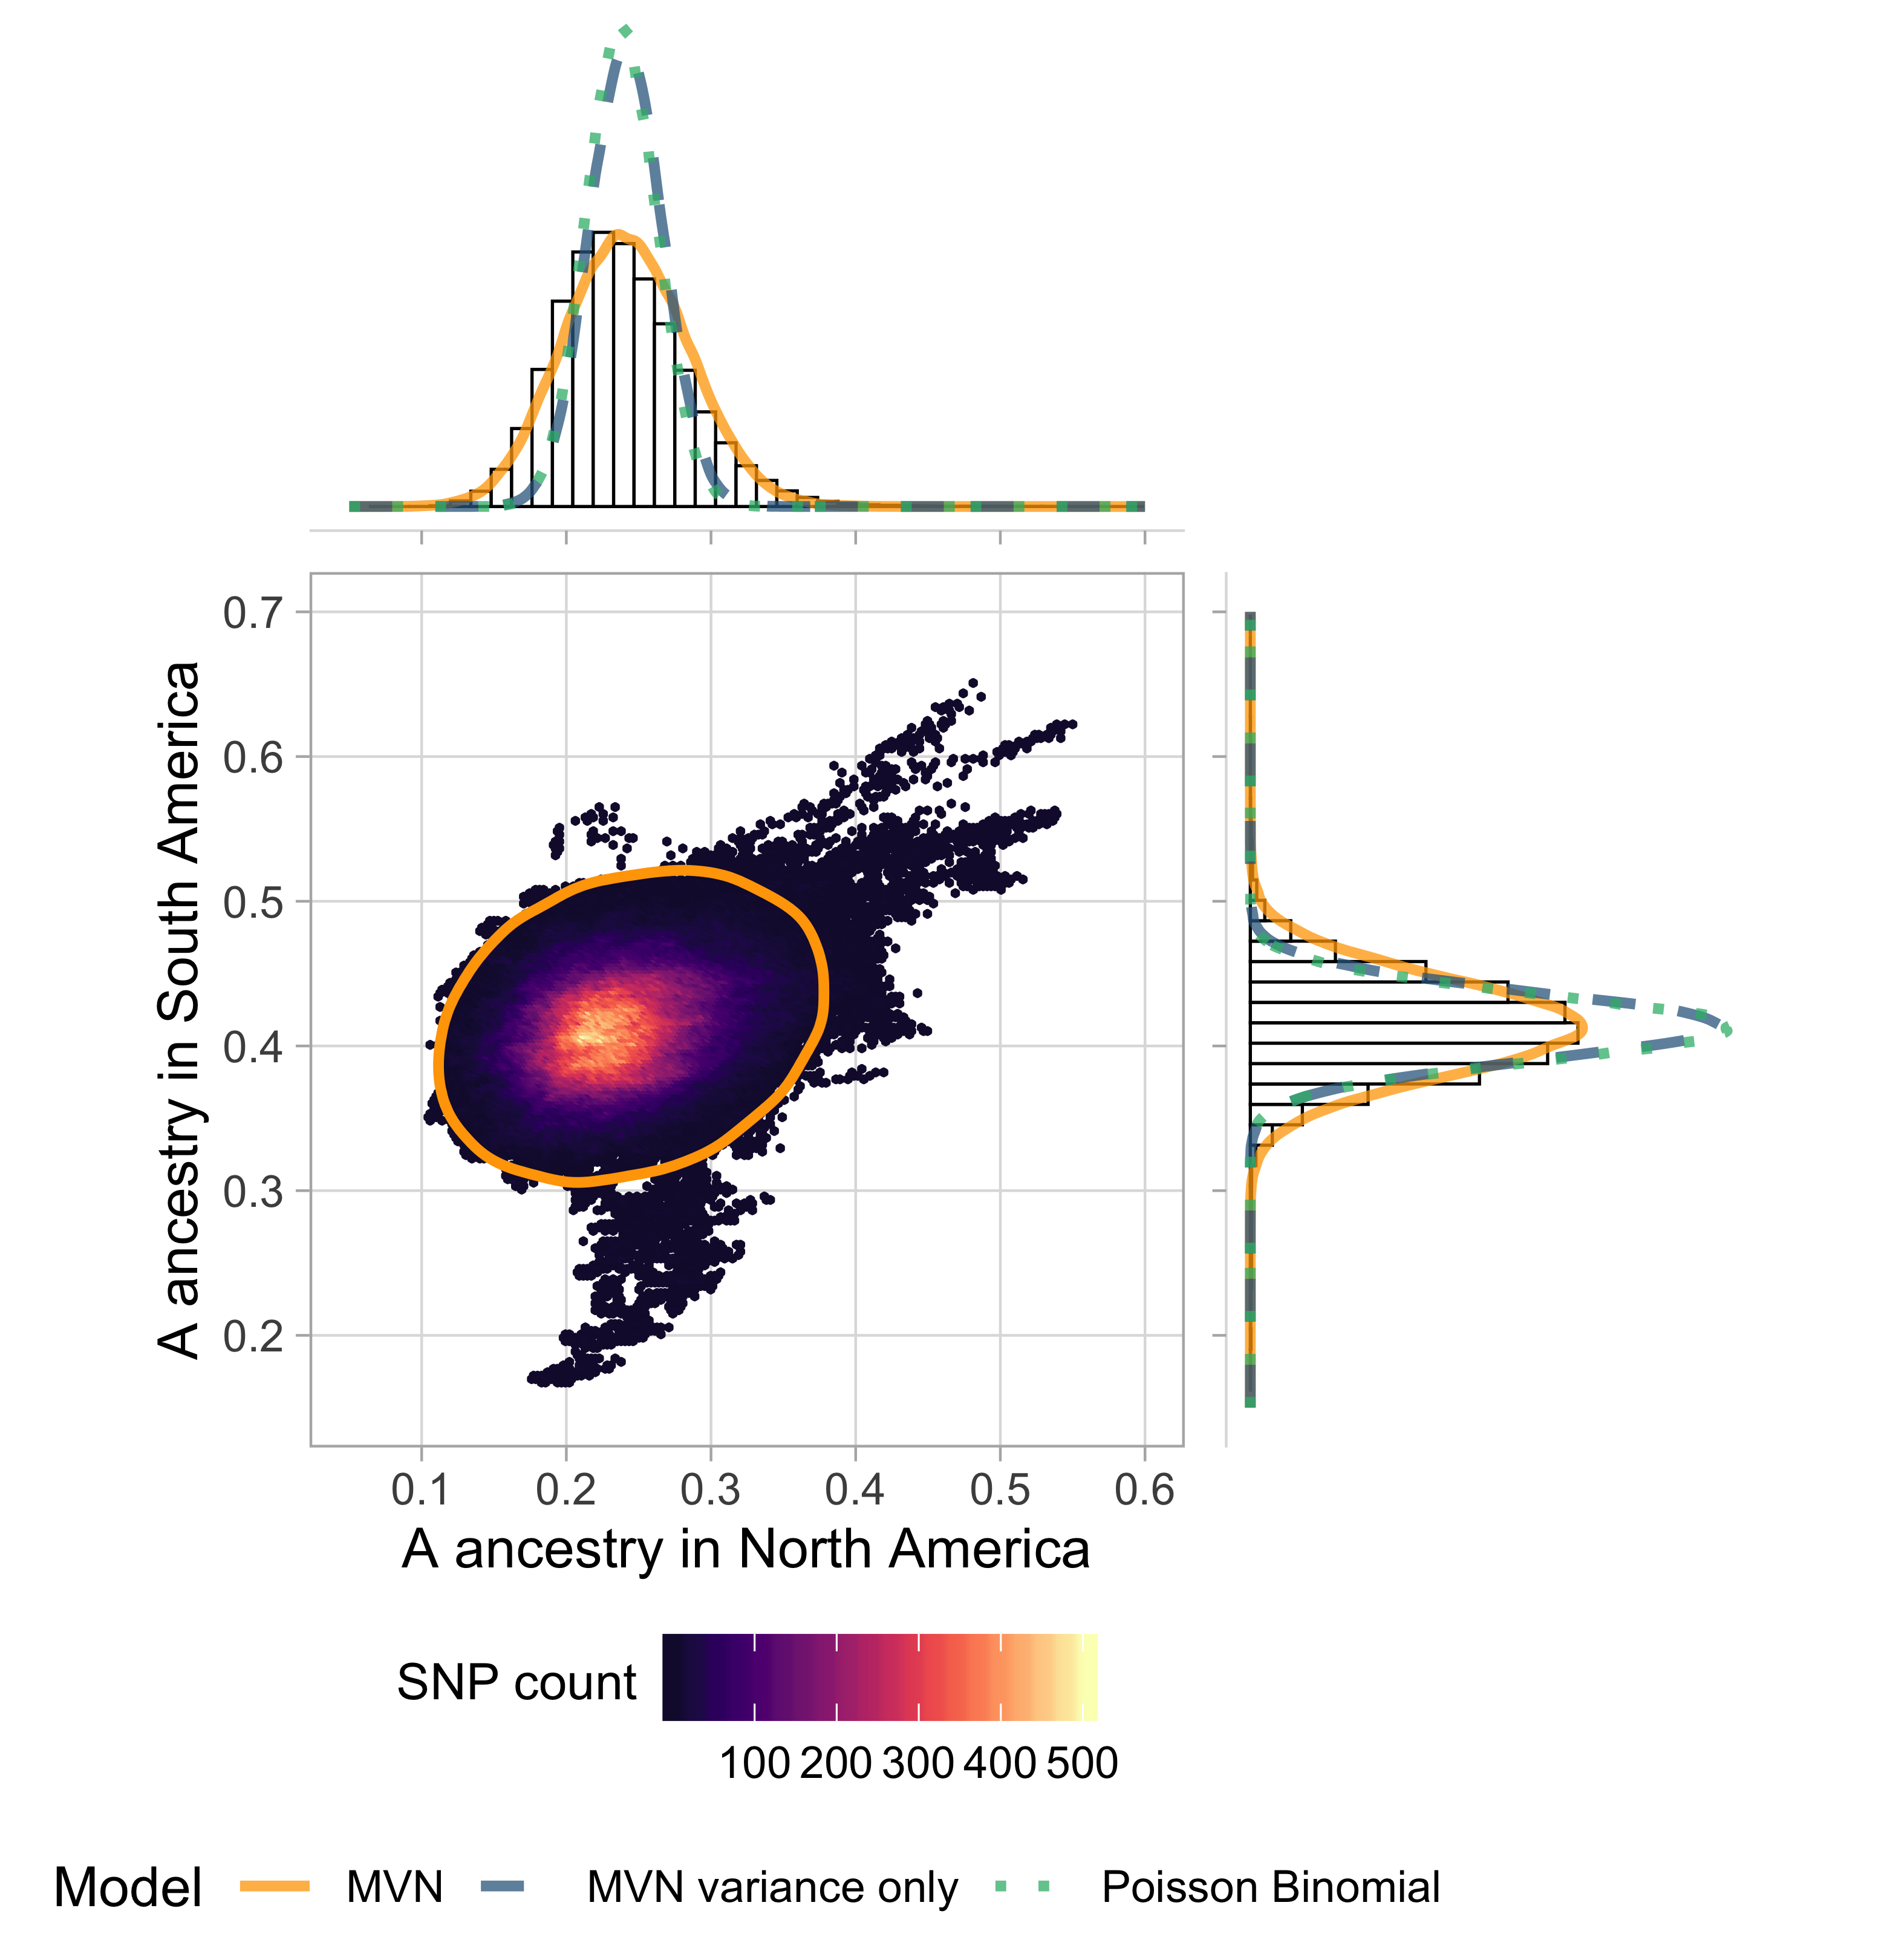
\includegraphics[width=.77\textwidth]{chapter1/figures/A_CA_vs_AR_density_marginal_hist.png}
\caption{ \textbf{Local ancestry outliers compared across hybrid zones.} We plot mean \A\ ancestry frequency in North vs. South America for 425k SNPs across the honey bee genome. SNPs are binned for visualization, and colored by the number of SNPs within each \ec{hexagon. The orange ellipse shows the approximate 99\% highest posterior density interval \ec{(HPDI)} based on the full MVN model, which accounts for drift in ancestry both within and between populations.
Using the same axes, we show the marginal histograms of \A\ ancestry for each continent separately (top and right panels). Imposed on these histograms we plot density curves for 3 possible null distributions for ancestry frequencies: the full MVN model, a variance-only MVN model which only accounts for drift within populations, and a Poisson binomial model which only includes sampling variance.
Most of the genome is consistent with neutrality under a MVN normal model of drift (98.6\% of SNPs fall within the orange ellipse), but there are also some clear outliers.} SNPs in the top right, with higher than expected \A\ ancestry proportions in both hybrid zones, are our best candidates for loci underlying adaptive \scutellata-ancestry associated traits. \ec{Note: While SNPs are thinned for LD, large outlier regions span many SNPs, which creates the streak-like patterns in the scatterplot.}}
\label{fig_A_CA_AR_density}
\end{figure}

Loci important to the successful invasion of \africanized\ \hyb\ honey bees are likely to have an excess or deficit of \scutellata\ ancestry across both continents. Thus, we tested separately for high and low \A\ ancestry outliers on each continent, and then identified overlapping outliers between the two hybrid zones. We find evidence of selection favoring \scutellata\ ancestry at 0.34\% of loci in N. America and 0.13\% of loci in S. America, across 14 chromosomes (Fig \ref{peaks}A). From these outliers, we find 13 regions with an excess of \A\ ancestry in both hybrid zones at less than a 10\% false-discovery-rate (top right corner of Fig \ref{fig_A_CA_AR_density}). The majority (11/13) of shared outliers co-localize within a $\sim$1.5Mb region on chromosome 1, but within this region outliers separate into multiple distinct peaks (Fig \ref{peaks}B). One way a cluster of \A\ ancestry peaks could form is if favored \scutellata\ alleles experience additional indirect selection from being in linkage disequilibrium with other favored \scutellata\ alleles at nearby loci, thereby increasing the total effective selection in a region \cite{Barton:1983fx}. While ancestry-informative markers (AIMs) with fixed or nearly fixed differences between \scutellata\ \ahb(\A) and both European \ahb{(C \& M)} ancestries are relatively rare, we were able to confirm the highest A peak within this cluster using AIMs outside of the local ancestry inference SNP set (Fig \ref{ACM_chr1_outlier_AIMs}). \A\ alleles at this main peak appear to have introgressed to high frequency hundreds of kilometers past the hybrid zone centers in both North and South America, but not reached fixation in any population (Fig \ref{top_snp_clines}). The rapid rise and slow fixation of \A\ \anc\ \ahb{at this locus} is potentially consistent with dominant fitness benefits. How far these \A\ alleles have introgressed past the present hybrid zones is currently unknown because they exceed our range of sampling.

\begin{figure}[ht]
\begin{center}
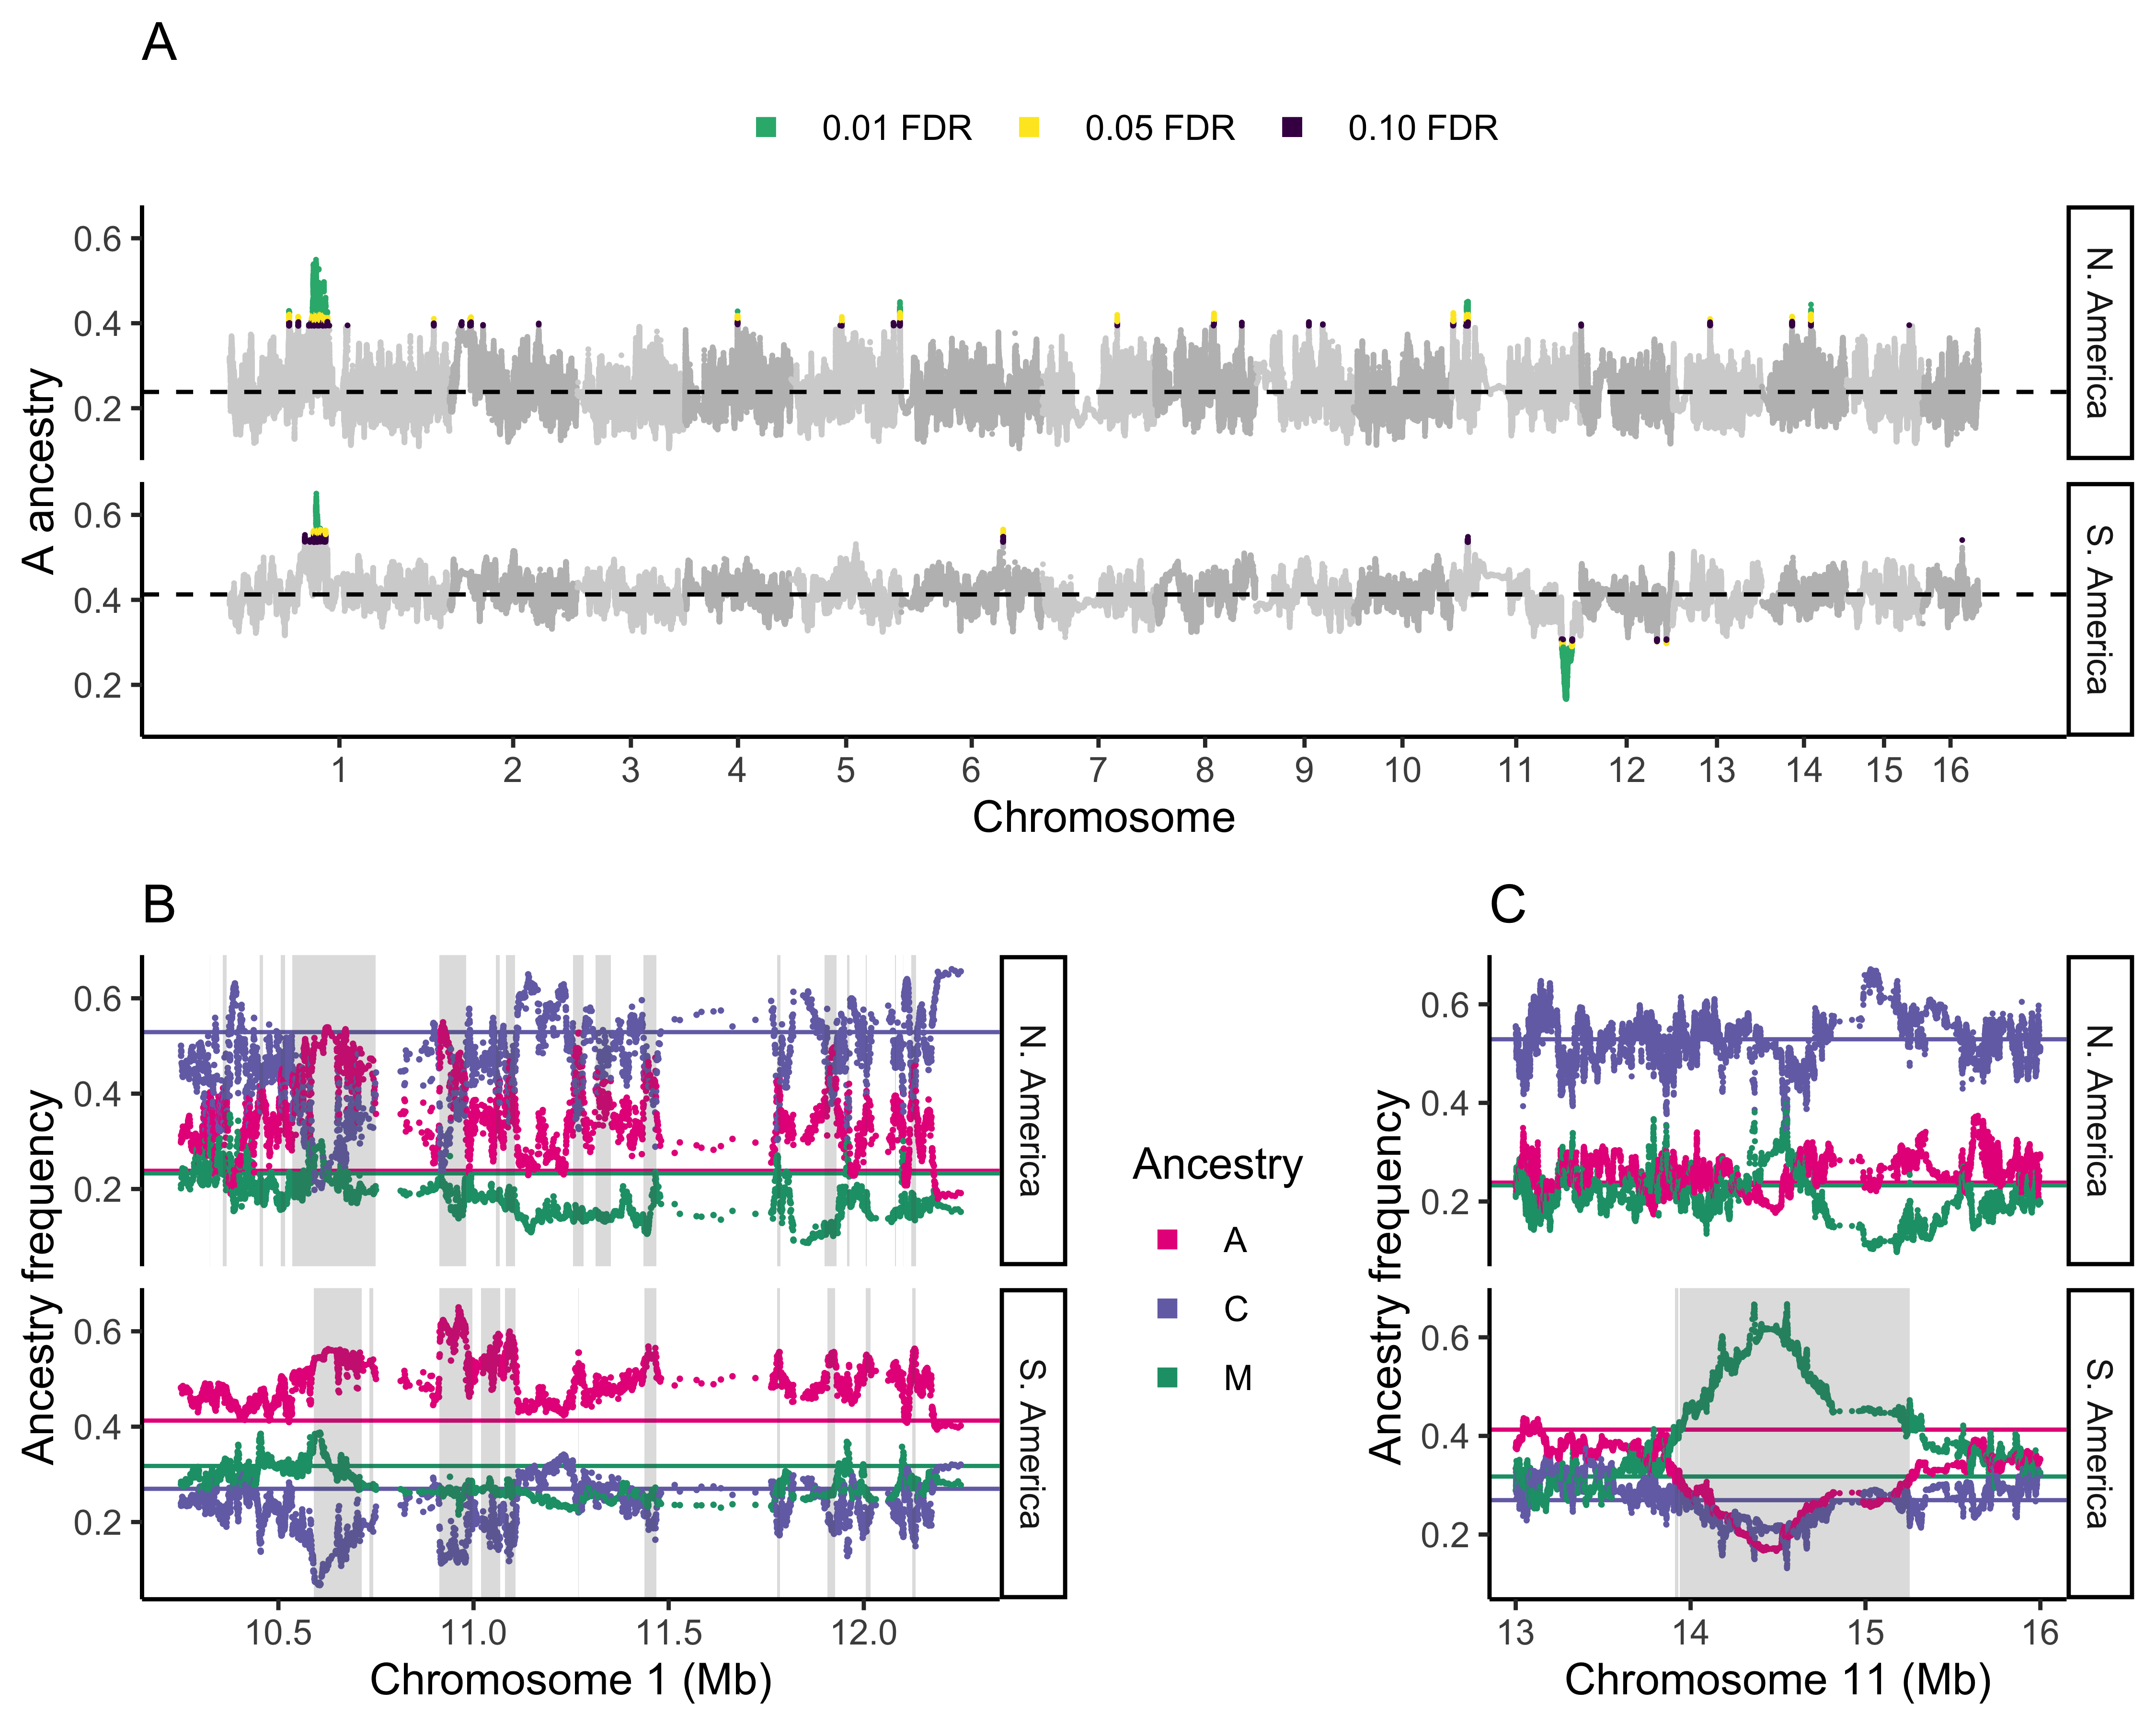
\includegraphics[width=0.9\textwidth]{chapter1/figures/A_outliers_grob.png}
\end{center}
\caption{ \textbf{Genomic location of ancestry outliers.} (A) Mean \scutellata\ (A) ancestry in each hybrid zone at SNPs across the genome, with outliers colored by their false-discovery-rate. Genome-wide mean \A\ ancestry in each zone is indicated with a dashed line. Shared peaks for high \A\ ancestry are seen on chromosomes 1 and 11; there are no shared peaks for low A ancestry. (B) Zoomed in view of cluster of shared high \A\ ancestry outliers on chromosome 1, with European ancestry separated into eastern (C) and western (M) subtypes. Genome-wide mean frequencies for each ancestry are shown with colored lines. Outlier regions meeting a 10\% FDR for high A ancestry are shaded in grey. Shared outliers between continents overlap between the top and bottom panels. (C) Zoomed in view of the high M European ancestry outlier region found in South America. Outlier regions for low \A\ ancestry ($<$10\% FDR) are shaded in grey. Note: The x-axis scale differs between plots.}
\label{peaks}
\end{figure}

\begin{figure}[ht]
%\begin{figure}[p]
\begin{center}
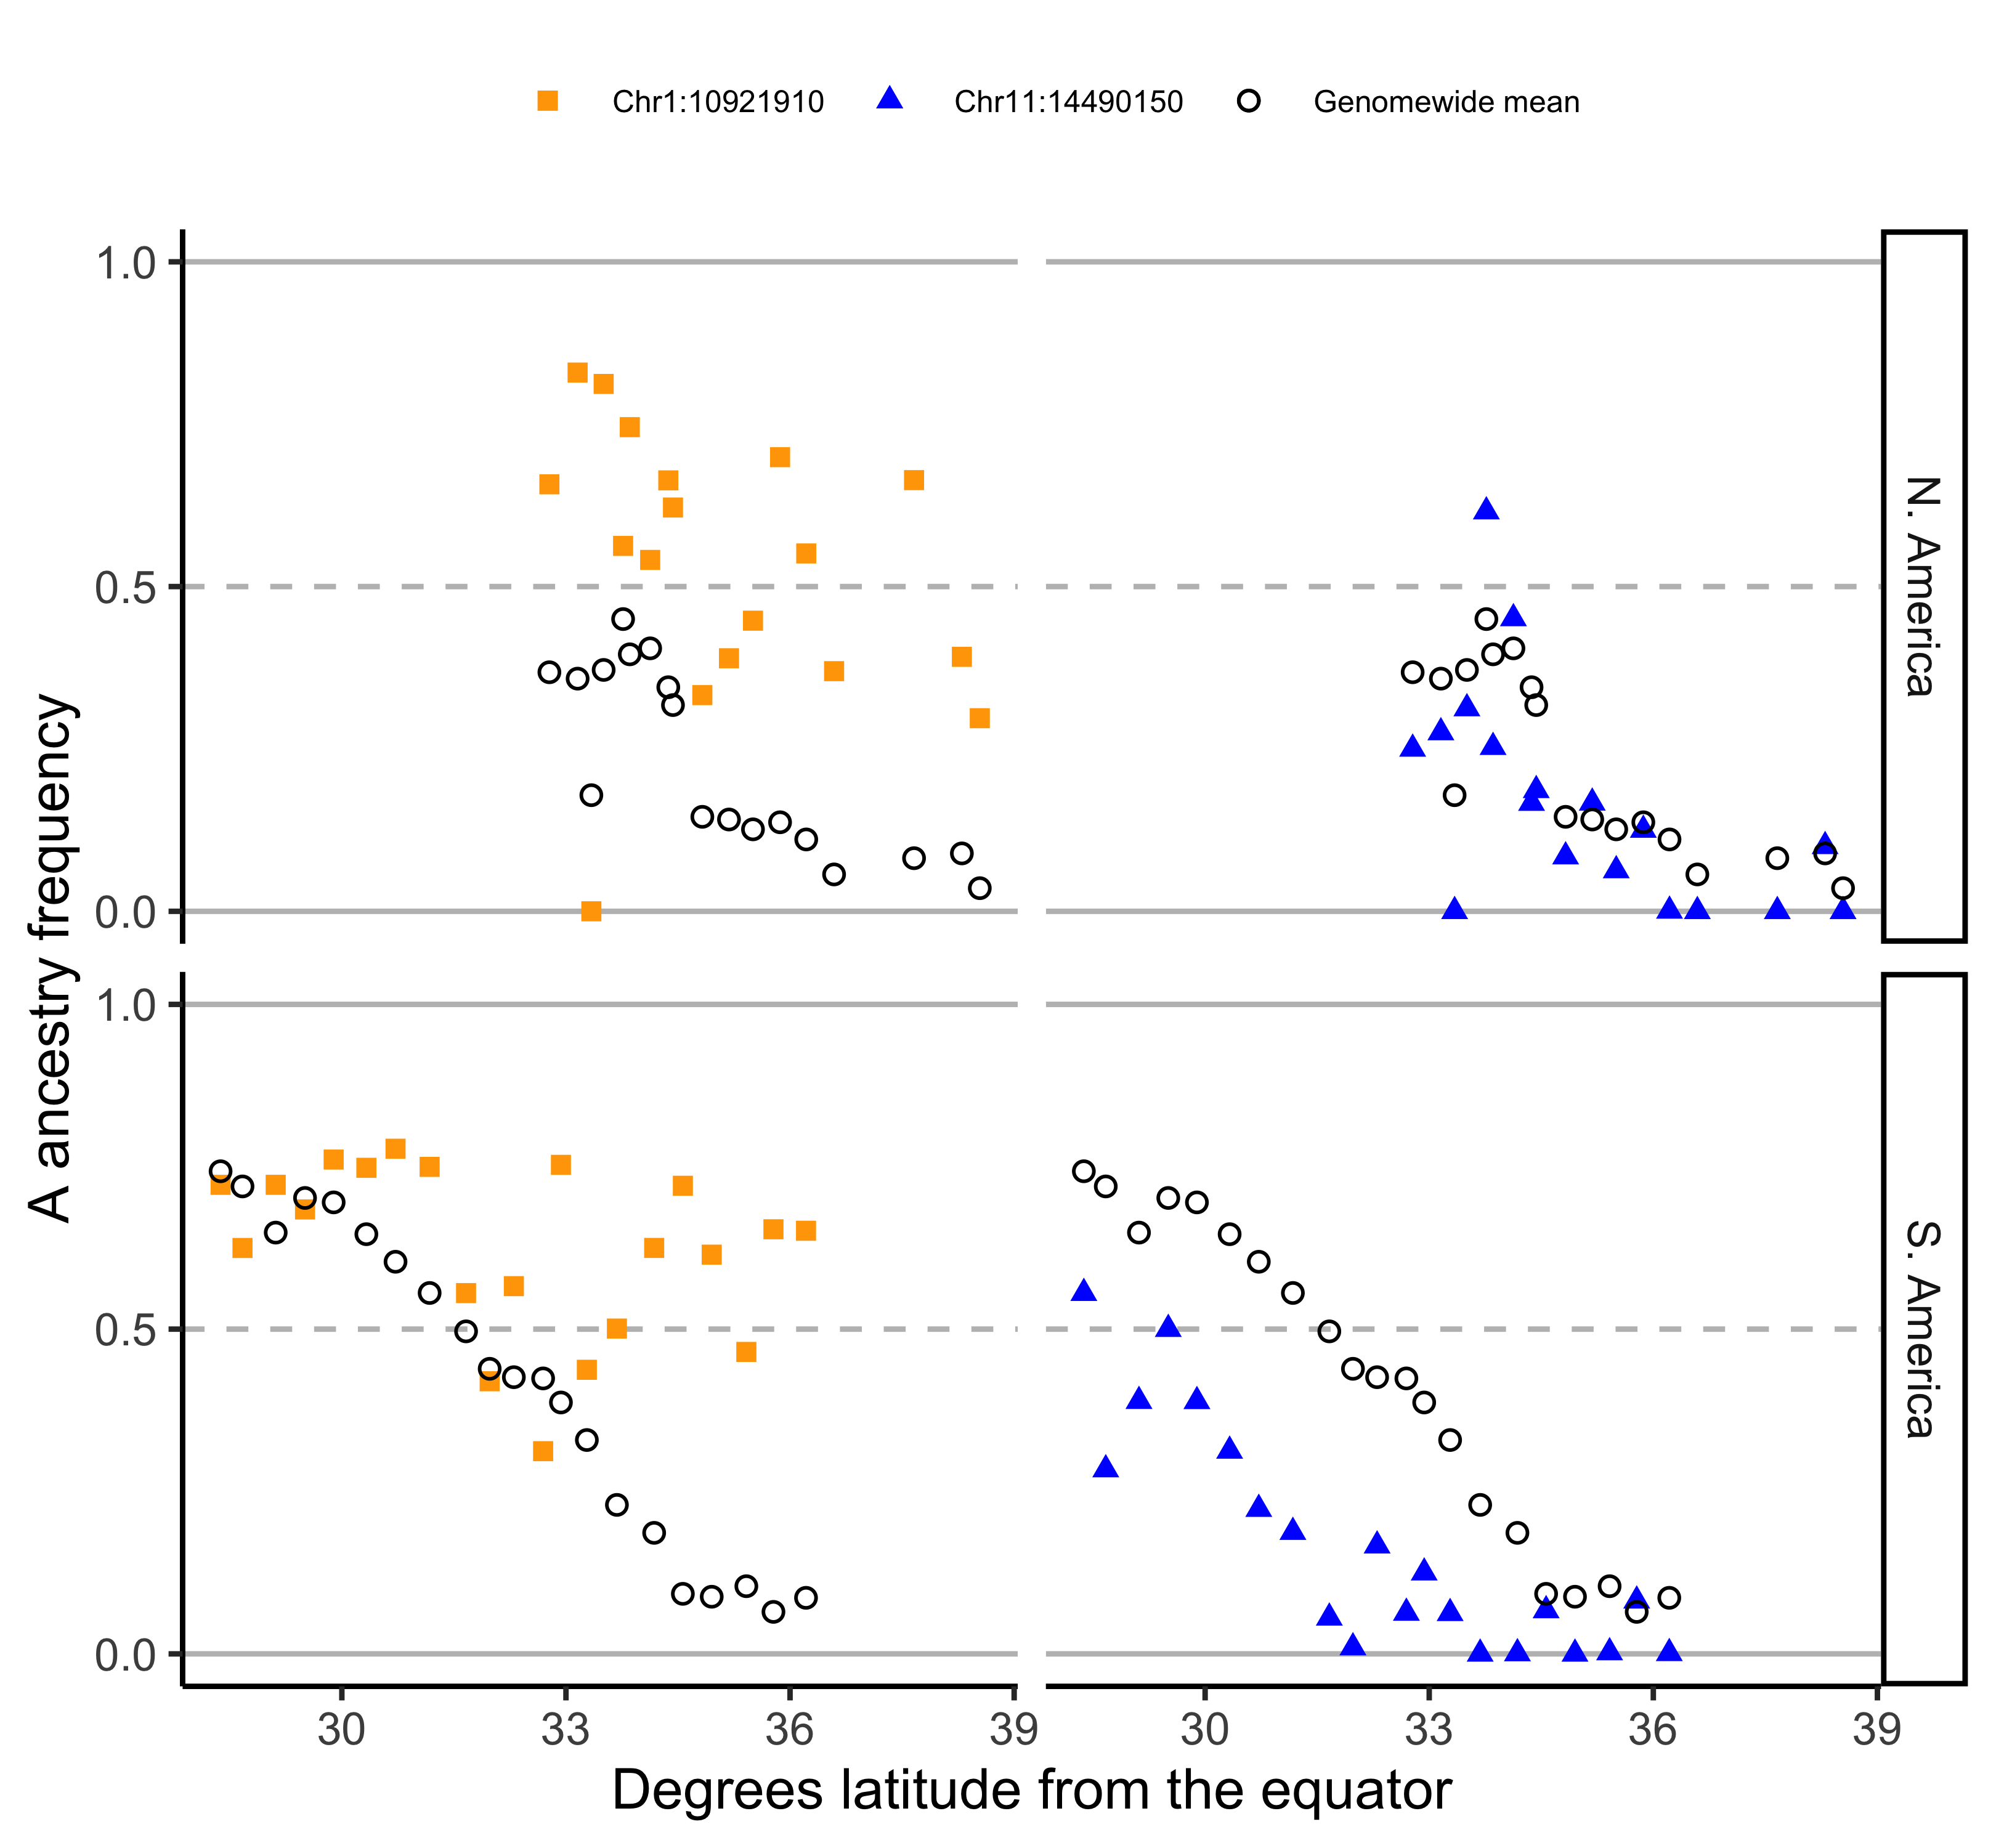
\includegraphics[width = .8\textwidth]{chapter1/figures/top_snp_clines.png}
\end{center}
\caption{ \textbf{Ancestry clines at outlier SNPs.} At two top outlier SNPs, we show the clines for mean population \scutellata\ (\A) ancestry across latitude in North (top) and South (bottom) America. To the left, we show the ancestry cline for the SNP with the highest \A\ ancestry in the combined sample, located within the top peak on chromosome 1 for high shared \A\ ancestry across continents. To the right, we show the ancestry cline for the SNP with the lowest \A\ ancestry in South America, located within the large outlier region on chromosome 11 for high M and low A ancestry. Genome-wide mean local ancestry calls for each population are shown for comparison as black circles.}
\label{top_snp_clines}
\end{figure}

Our goal was to identify regions of the genome where high fitness is broadly associated with \scutellata\ ancestry, but an alternative explanation for high \A\ ancestry at a locus is that a very recent adaptive mutation just happened to fall on an \A\ haplotype, initiating a classic ‘hard sweep'. For shared high \A-ancestry outlier regions, we distinguished between these two scenarios using population differentiation (F\textsubscript{ST}) within A ancestry. We analyzed differentiation across the large cluster of shared high \A-ancestry outlier peaks on chromosomes 1 and across a smaller region on chromosome 11 that contains the other two high \A\ ancestry outliers shared between continents. We did not find high allelic differentiation between North and South American A ancestry tracks and the \scutellata\ \A\ reference panel \ahb{from Africa} (Figs \ref{fst_chr1_A_outlier} and \ref{fst_chr11_A_outlier}), suggesting that \scutellata\ ancestry in general, and not one particular haplotype, was favored by natural selection at these loci.

We used previous literature and gene orthologs to identify possible adaptive functions for regions of the genome where selection has favored \scutellata\ ancestry. There are 3 major quantitative trait loci (QTLs) associated with defense behaviors (e.g. stinging) in genetic crosses of \ahb{defensive} \africanized\ \hyb\ \ahb{honey bee colonies} and \ahb{low-defense} European \ahb{colonies} \cite{Hunt:1998th, Hunt:2007im}, none of which overlap any signatures of selection from this study. No studies have mapped the genetic basis of elevated \textit{Varroa} defense in \africanized\ \hyb\ (vs. European) bees, but we were able to compare our results to quantitative trait loci (QTLs) associated with anti-\textit{Varroa} hygiene behaviors \cite{Tsuruda:2012fa, Oxley:2010dw, Spotter:2012dx} and defensive grooming \cite{ArechavaletaVelasco:2012cm} more generally. The cluster of peaks for high shared \A\ ancestry on chromosome 1 overlaps a putative QTL associated with removal of \textit{Varroa}-infested brood \cite{Spotter:2012dx}, but there are a number of large QTLs in the genome. A total of 104 genes overlap high \A\ ancestry outlier peaks. Predicted functions for these genes (primarily based on fly orthologs) are not significantly enriched for any Gene Ontology (GO) categories, which may simply reflect that many outlier regions are broad and contain many genes, most of which are likely unrelated to their rise in ancestry frequency. A smaller set of 37 genes with high \A\ ancestry have signatures of selection on both continents. For these, we searched the literature and found that two have been associated with \textit{Varroa} in previous studies: a myoneurin (LOC725494) that is overexpressed in the brains of \textit{Varroa} infected worker bees compared to \textit{Nosema} infected bees and controls \cite{McDonnell:2013ej} and an uncharacterized protein (LOC725683) that is over-expressed in parasitized drones compared to non-parasitized drones \cite{Surlis:2018cb}. While these are potentially intriguing candidates for selection, \textit{Varroa} is only one of many possible selective pressures, and more work is needed to link the signals of selection we find here to adaptive functions.

In contrast to high \A\ ancestry outliers, we do not find any shared outliers for European ancestry. However, the most striking example of a single-zone selection event is a large 1.4Mb region on chromosome 11 with excess European ancestry in South America (bottom middle of Fig \ref{fig_A_CA_AR_density}). This region was previously identified to have low \A\ ancestry in \africanized\ \hyb\ honey bee populations from Brazil \cite{Nelson:2017cj}. We independently identify this region as a low-\A\ ancestry outlier across Argentina, using different A/C/M reference bees, ancestry calling algorithm, and bee samples than the previous paper. We find that populations across the South American hybrid zone have reduced \A\ ancestry at this locus, but that North American populations do not appear to have experienced selection (Fig \ref{top_snp_clines}). By including C-lineage diversity in our admixture analysis, we additionally show that this region is specifically elevated for M haplotypes, and not European haplotypes more broadly (Fig \ref{peaks}C). This region has many diverged SNPs between the three ancestry groups beyond the SNPs included in our ancestry\_hmm analysis, which we use to confirm high rates of M introgression (Fig \ref{ACM_chr11_outlier_AIMs}). It does not appear that a new mutation or narrow set of haplotypes was favored within M because we see little differentiation between the M ancestry in this selected region compared to the M reference panel. Additionally, within the selected region we find a peak of high F\textsubscript{ST} between A, C, and M reference panels (Fig \ref{fst_chr11_M_outlier}), which is consistent with this region having historically been under selection within these ancestry groups. Finally, the California bees do not have a significant deficit of \A\ ancestry like the Argentinian bees do, but they do have two narrow peaks of excess M ancestry within this region, in the top 3\% and 7\% empirical percentiles for M ancestry genome-wide. Our data support a scenario in which a diversity of M haplotypes carrying the favored allele were driven to high frequency in South America after \africanized\ \hyb\ honey bees spread north of Brazil. Potential candidate genes specific to this large M-ancestry outlier region on chromosome 11 are previously described by \cite{Nelson:2017cj}. In total, we find 186 genes that overlap low-\A\ ancestry outlier peaks ($<$10\% FDR). These genes are not functionally enriched for any Gene Ontology (GO) categories.

\section*{Discussion}

The introduction of \ahb{\textit{scutellata}} honey bees to Brazil in the 1950s sparked one of the largest and best studied biological invasions known to date, \ahb{with \africanized\ hybrids} spreading from a single point of release over much of the Americas in less than 50 years. We add to this literature the first comparative study of the invasions in North and South America, with genome-wide resolution on the present distribution of \scutellata\ \ahb{(A)} ancestry.

The parallel alignment of the genome-wide cline with latitude in both continents, despite very different length dispersal routes, strongly supports the view that \scutellata\ ancestry has reached a stable climatic range limit. Because our transect in California only covered the upper half of the North American cline, the full shape for this genome-wide cline is uncertain, and may be asymmetrical because one signature of a moving hybrid zone is elongation of the lagging tail \cite{buggs2007empirical}. In contrast, we have strong evidence for convergence in the  low-\A\ portions of these two genome-wide clines, which are not expected to be distorted by cline movement, and reflects similar latitudinal range limits for \scutellata\ ancestry in North and South America. Global warming trends could shift the location of the observed clines towards the poles, as has been documented for other hybrid zones sensitive to climate change \cite{Taylor:2015dq}. While we currently lack temporal data with comparable genomic and geographic resolution, our results can be used as a baseline for future study.

Significant effort has been focused on finding an environmental isocline that divides regions where \africanized\ \hyb\ honey bees are expected to dominate and regions where they cannot overwinter (e.g. \cite{TaylorJr:1984vg, Southwick:1990cq, Sheppard:1991ep, Harrison:2006gk}). However, we observe ancestry clines that are hundreds of kilometers wide, not the narrow clines created by strong selection across a discrete environmental transition. Theoretically, these broad clines could be consistent with neutral diffusion of ancestry by migration over tens of generations. However, a scenario of neutral diffusion is inconsistent with external evidence of the rapid spread of the invasion and strong fitness trade-offs with climate: the high competitive advantage and very rapid advance of \scutellata\ahb{-associated traits and \A\ mitochondria} in the tropics in the face of considerable interbreeding with European bees and, conversely, documented low fitness \ahb{of \africanized\ hybrids} in cooler climates, with low overwinter survival and maladaptive metabolic efficiency, foraging preferences and nesting behaviors (see \cite{Harrison:2006gk} for a review).  Thus, we conclude that honey bee fitness is more likely to be tracking environmental variables with smooth transitions over broad geographic regions (e.g. climate), which may create intermediate environments where ancestry intermediates have higher fitness, thus broadening the observed hybrid zones. \ec{These proposed dynamics are similar to well-studied cases in other systems where bounded hybrid superiority and/or local adaptation to continuous environments maintain adaptive clines across broad geographic regions (e.g. \cite{good2000bounded,de2014adaptation,Adrion:2015ko})}.

As a null model, we expect phenotypic clines to match the scale of the observed ancestry clines, with smooth transitions in mean phenotype over hundreds of kilometers. Many phenotypes of interest, e.g. defensive behavior or \textit{Varroa} tolerance, are expressed or measured at the colony-level and so we could not assess these in our survey of freely foraging bees. Future phenotypic surveys could be compared with our genomic clines to ascertain if key phenotypes diverge from this expected pattern, e.g. due to strong selection beyond that experienced by the rest of the genome. Indeed we see that wing length, a trait hypothesized to be associated with latitudinal body-size adaptation following Bergmann's rule \cite{Daly:1991de}, has a geographic distribution consistent with the genome-wide ancestry cline. This suggests that while wing length, which is strongly correlated with body size \cite{Daly:1978hu,Rinderer:86a}, may well have fitness trade-offs with climate, selection for these traits does not appear to be strong enough compared to average selection for ancestry to deviate from background genomic patterns over a short time scale.

We observe relative uniformity at the climate barrier, with no individual loci showing steeper ancestry clines than what can be produced by a null model accounting for background patterns of variation in ancestry frequencies shared across populations. Nor do we observe any loci that have below 10\% frequency of \A\ ancestry in California, despite the large distance and climatic range traveled over by this portion of the invasion. If the invasive ability of \africanized\ \hyb\ \ahb{honey} bees were due to a small number of loci we would expect \scutellata\ ancestry to have been swamped out at many unlinked neutral loci in the genome due to interbreeding at the front of the advancing wave of expansion \cite{currat2008hidden}. Instead, relative genomic cohesion points to a \ec{polygenic} basis for the high fitness and rapid spread of \scutellata\ ancestry as well as the fitness costs in cooler climates underlying the parallel range limits observed across continents. However, we note that the distinction between \ahb{so-called ‘Africanized’ and ‘non-Africanized’} honey bees is likely to further blur over time. Genetic barriers are strengthened when selection is distributed across many loci, but they are still easily permeated by adaptive alleles \cite{Barton:1986wp}. Furthermore, given high recombination rates in honey bees, we predict only loci tightly associated with climate-based fitness trade-offs will remain geographically bounded over long periods of time.

\ecec{Our findings add to the genomic evidence that \africanized\ \hyb} honey bees cannot be treated as a single genetically and phenotypically cohesive group. \ecec{We show that bees have intermediate \scutellata\ ancestry proportions over large geographic areas, with no evidence that \africanized\ \hyb\ honey bees share any defining \scutellata\ \anc\ loci (including mtDNA). Colonies within these wide hybrid zones have largely unknown colony-defense behaviors and are likely to show high variance in many traits, overlapping with variation within European bees. These bees defy ‘Africanized’ (vs. ‘non-Africanized’) labels currently used by researchers, beekeepers, and policy makers. While more precise ancestry information is becoming increasingly available, it's important to understand the limitations for trait prediction. Importantly, there is no one-to-one mapping between \A\ ancestry and colony defense. Recent findings show that both \scutellata\ and M European ancestry contribute to defensiveness segregating in \africanized\ hybrid populations in Brazil \cite{Harpur:2020}.} \ecec{Additionally, ‘gentle Africanized honey bees’ in Puerto Rico show that \africanized\ \hyb\ honey bee populations can evolve low defense while maintaining \scutellata\ ancestry and other associated traits \cite{RiveraMarchand:2012gn, Avalos:2017jb}. Future research could improve upon ancestry-based trait predictions by identifying genetic markers for agriculturally undesirable and beneficial traits segregating in \africanized\ \hyb\ honey bee populations.}

\ahb{\textit{Scutellata}-European hybrids} provide a promising source of genetic variation for breeding in light of the vulnerability of European lineages to current environmental stressors and associated bee declines \cite{Goulson:2015er}. \ahb{\textit{Scutellata}-European hybrid} honey bees have high competitive fitness and, we show here, maintained high genetic diversity despite their rapid expansion. In this study, we have taken a first step towards mapping the genetic basis of the high fitness of \africanized\ \hyb\ honey bees by identifying loci where selection has favored \scutellata\ or European ancestry in both North and South America. We identify several loci with convergently high \A\ ancestry on both continents, and many more across the genome with evidence of selection favoring \A\ ancestry in one hybrid zone. In contrast, with the exception of one striking outlier for high M ancestry in South America, we find little evidence that European ancestry or admixture per se contributed broadly to the success of \africanized\ \hyb\ honey bees.
We attribute this difference in results from a previous study of \ahb{\textit{scutellata}-European hybrid} honey bees in Brazil \cite{Nelson:2017cj} to a more appropriate null model that accounts for shared variance in ancestry across populations. While our population genetics approach is trait-blind, our results can be compared to future functional and genetic mapping studies to look for overlap between trait-associated and positively selected loci. Applying similar methods to other systems, especially where replicated hybrid zones can be sampled, holds great promise for revealing loci important to adaptation.


\section*{Materials and Methods}
\ec{Statistical results and figures were created in R \cite{R:2019} with use of the tidyverse \cite{R_tidyverse} packages. Other scripts were run using GNU parallel \cite{tange:2018parallel}.}

\subsection*{Sampling}
We sampled individual foraging honey bees across two hybrid zones, located at the transitions to temperate climates in North and South America. We sampled at least 10 bees each from 12 populations in California and 21 populations in Argentina (see maps, Fig \ref{fig_map}).

For each population, we hand-netted individual foraging bees within a sampling radius of approximately 15km. Because commercial colonies are often temporarily relocated for the spring pollination season, we sampled in summer, when foraging bees are more likely to come from resident populations. We additionally included in our analyses 35 high-coverage published genomes of freely foraging bees collected from 6 populations between September 2014 and January 2015: Davis, Stebbins, Stanislaus, Avalon (Catalina Island), Placerita, and Riverside (Sky Valley and Idyllwild) \cite{Cridland:2018fx}.
While these sampled bees come from an unknown mixture of local feral and domesticated colonies, previous surveys from California have found that freely foraging bees tend to closely match feral sources, based on mtDNA composition \cite{Kono:2015fi}. Consistent with this view, eight of our sequenced bees from different populations in Argentina were collected close to a feral nest ($<5$m), but do not appear to be ancestry outliers for their sampling locations. More specifically, we fit a general linear model (logit(\A\ ancestry) $\sim$ absolute latitude + feral nest) using glm with gaussian errors in R and found no significant effect on \A\ ancestry of sampling near a feral nest ($P = 0.97$). Based on these results and our seasonal timing, the bees in this study are likely sourced primarily from local feral populations, with some contribution from resident domesticated bee colonies.

\subsection*{Lab work and sequencing}
We selected a subset of 279 bees from our North and South American hybrid zones for whole genome sequencing, 8-9 bees per sampled population (see \nameref{table_bee_gps}). For each bee, we dissected wing flight muscles from the thorax and extracted DNA using QIAGEN DNeasy Blood and Tissue kits. We followed a new high-throughput low-volume DNA library preparation protocol (see \cite{Rowan:2019} for details, “Nextera Low Input, Transposase Enabled protocol"). Briefly, we prepared individual Nextera whole-genome shotgun-sequencing DNA libraries using enzymatic sheering and tagmentation. Then we PCR-amplified and barcoded individual libraries using the Kapa2G Robust PCR kit and unique custom 9bp 3’ indices. Finally, we pooled libraries within each lane and ran bead-based size-selection for 300-500bp target insert sizes. We targeted 4-6x coverage per bee based on a preliminary analysis of our power to replicate local ancestry calls from one of the published high coverage populations (Riverside 2014) using simulated low coverage data (Fig \ref{sims_downsample}). We multiplexed our samples across 5 Illumina HiSeq4000 lanes for paired-end 2 x 150bp sequencing. In total, we generated 5.1x mean coverage per bee for 278 samples. The 279th sample was excluded from all analyses for having extremely low (\textless 0.1x) sequence coverage.

\subsection*{Alignment and SNP set}
In addition to the sequence data produced by this study, we downloaded Illumina raw read sequences for 35 previously published California genomes (PRJNA385500 \cite{Cridland:2018fx}) and a high-quality reference panel of  \ahb{\textit{A. m. scutellata} (A,} n = 17), \ahb{\textit{A. m. carnica} (C,} n = 9), and \ahb{\textit{A. m. mellifera} and \textit{A. m. iberiensis} (M,} n = 9) honey bee genomes (PRJNA216922 \cite{Harpur:2014ei} and PRJNA294105 \cite{Cridland:2017el}) from the NCBI Short Read Archive. For all bees, we mapped raw reads to the honey bee reference genome HAv3.1 \cite{Wallberg:2019fd} using Bowtie2 very-sensitive-alignment with default parameters \cite{Langmead:2012jh}. We then marked and removed duplicate reads with PICARD and capped base quality scores using the ‘extended BAQ' option in SAMtools\ec{\cite{Li:2009samtools}}. Using the software ANGSD \cite{Korneliussen:2014_ANGSD}, we identified a set of SNPs with minor allele frequency $\geq$ 5\% in the combined sample based on read counts (-doMajorMinor 2 -doCounts 1). We excluded unplaced scaffolds (\textless 5Mb total) and applied standard quality filters for SNP calling (base quality $\geq$ 20, mapping quality $\geq$ 30, total read depth $\leq$ 5500 ($\sim$2x mean), and coverage across individuals $\geq$ 50\%). We calculated the genetic position (cM) for each SNP using a 10kb-scale recombination map \cite{Jones:2019wg} and linear interpolation in R (approxfun). We assumed constant recombination rates within windows and extrapolated positions beyond the map using the recombination rate from the nearest mapped window on that chromosome.

We identified SNPs on the mitochondria (HAv3.1 scaffold NC\_001566.1) using the same pipeline as nuclear DNA above, but allowing for extra read depth (up to 100000000x). We then called consensus haploid genotypes at these SNPs for all individuals using ANGSD (-dohaplocall 2 -remove\_bads 1 -minMapQ 30 -minQ 20 -doCounts 1 -minMinor 2 -maxMis 174).

\subsection*{Global ancestry inference}
We estimated genome-wide ancestry proportions for each bee using methods designed for low-coverage sequence data. Briefly, we combined bee genomes from the hybrid zones with reference genomes \ahb{for} \scutellata\ (A), eastern European (C) and western European (M) \ahb{bees}. To reduce linkage disequilibrium (non-independence) between our markers for global ancestry inference, we thinned to every 250th SNP ($\sim$14k SNPs at 19kb mean spacing) before calculating genotype-likelihoods for each bee using the SAMtools method in ANGSD (-GL 1). We first ran a principal components analysis in PCAngsd \cite{Meisner:2018_pcangsd} to confirm that genetic diversity in the hybrid zones is well-described by 3-way admixture between A, C, and M reference panels (Fig \ref{supp_pca}). We then estimated genome-wide ancestry proportions for all bees using NGSAdmix (K = 3) \cite{Skotte:2013_NGSadmix}.

\subsection*{Local ancestry inference}
We inferred the mosaic of \scutellata\ vs. European ancestry across the genome of each bee using a hidden Markov inference method that can account for \scutellata\ (A), eastern European (C) and western European (M) sources of ancestry within low-coverage \africanized\ \hyb\ honey bee genomes (ancestry\_hmm \ec{v0.94} \cite{CorbettDetig:2017gh}). For local ancestry inference, we enriched for ancestry-informative sites by filtering for $\geq$ 0.3 frequency in one or more reference population (A, C, or M) and at least 6 individuals with data from each reference population. We subsequently thinned markers to 0.005cM spacing, because at that distance linkage disequilibrium within ancestries is expected to be low ($r^{2} < 0.2$ \cite{Wallberg:2014ha}), leaving a final set of 542,655 sites for ancestry calling, or $\sim \nicefrac{1}{7}$ of the original SNP set. Individual bees sequenced in \ec{this study} and previously published California bees have 5.42x and 14.5x mean coverage, respectively, across this final SNP set. For each population, we jointly estimated time since admixture and ancestry across the genome of each individual, using read counts from the hybrid zone and allele frequencies for \ahb{A, C and M} reference populations at each SNP. To generate major/minor allele counts for each reference population, we used ANGSD to call genotypes (-doPost 1) using a minor allele frequency prior (-doMaf 1) and the SAMtools genotype likelihood (-GL 1), after quality filtering (map quality $\geq$ 30, reads matching major/minor allele $\geq$ 60\%, and read depth $\geq$ 6x). As additional inputs to ancestry\_hmm, we used NGSAdmix results as a prior for population ancestry proportions and set the effective population size to ${N_e}=670,000$ \cite{Nelson:2017cj}. We modelled a simple three-way admixture scenario: starting with C ancestry, we allowed for a migration pulse from M and a second, more recent, migration pulse from A. Timing of both migration pulses were inferred from the range 2-150 generations, with priors set at 100 and 60 generations. To calculate a point estimate for each individual's ancestry proportion at a SNP, we marginalized over the posterior probabilities for homozygous and heterozygous ancestry from the ancestry\_hmm output (i.e. $A = p(AA) + \nicefrac{1}{2}(p(CA) + p(MA)$).

\subsection*{Ancestry covariance matrix}
To explore how populations vary and covary in their \scutellata\ ancestry along the genome we calculated the empirical population ancestry variance-covariance matrix ($K$), an admixture analog of a genotype coancestry matrix (e.g. \cite{Thornton:2012kz}). The $K$ matrix is calculated using population \scutellata\ \ahb{(A)} ancestry frequencies inferred by the local ancestry HMM, e.g. for populations i and j with mean ancestry proportions $\alpha_i$ and $\alpha_j$, and ancestry frequencies at a locus $anc_{i,l}$ and $anc_{j, l}$, their ancestry covariance calculated across all L loci genome-wide is
\begin{align*}
K[i, j] = \frac{1}{L} \sum_{l=1}^{L} (anc_{i,l} - \alpha_i)(anc_{j,l} - \alpha_j).
\end{align*}

\subsection*{\ec{Ancestry correlations between the high-latitude cline endpoints}}
\ec{To more formally test for excess ancestry correlations between more geographically distant (but climatically similar) populations, we grouped populations by dividing each hybrid zone into low- and high-\A\ ancestry regions relative to the estimated latitude for the genome-wide cline center. The southernmost 11 (out of 20) of the South American populations, and all of the sampled North American populations, fall in the ‘low A' half of their respective hybrid zones. We calculated mean ancestry covariances (K matrices) separately for each chromosome, using the genome-wide mean ancestry as $\alpha$, then summarised across populations by taking the mean correlation for each type of pairwise comparison, within and between continents and regions. We tested whether, on average across chromosomes, low-A South American populations share higher ancestry correlations with low-A North American populations than with geographically closer high-A South American populations and repeated this test excluding chromosomes 1 and 11 which contain large outlier regions (Fig \ref{fig_mean_k_by_chr}). We also tested the same group comparison across recombination rate quintiles instead of chromosomes (Fig \ref{fig_mean_k_by_r}).

To investigate whether recent long-distance migration likely generated the elevated ancestry correlations we observe between low-A South America and low-A North America, we looked at patterns of allelic covariance within ancestry. Specifically, for each ancestry we estimated a genetic covariance matrix in PCAngsd for all individuals sampled from the hybrid zone, based on allelic diversity within high-confidence homozygous ancestry tracts (posterior \textgreater 0.8). Under recent migration, we would expect the excess \A\ ancestry correlations between the two ends of the hybrid zones to be mirrored by allelic covariances within all three ancestries. Instead, we find that the two most prevalent ancestries, A and C, both have low or negative genetic covariances between continents (Fig \ref{cov_within_anc}). In contrast, M ancestry does show an excess of cross-continent covariance, and we followed up to determine if this is uniquely American covariance (i.e. the result of shared drift within the Americas) or could have been imported from Europe. Adding reference individuals to these within-ancestry analyses, we find that M ancestry in the Americas imported pre-existing structure from Europe, with more Poland-like (\textit{Apis mellifera mellifera}) than Spain-like (\textit{Apis mellifera iberiensis}) M ancestry at the temperate ends of the clines (Figs \ref{pca_within_anc} and \ref{pc1_anc_by_lat}).}

\subsection*{Simulated ancestry frequencies}
At various points in the results we compare our outliers to those generated by genome-wide null models of ancestry variation along the genome. We simulated variation in ancestry frequencies at SNPs across the genome under three models: (1) A \edit{P}oisson-binomial model that only accounts for sampling variance, not drift (e.g. \cite{Nelson:2017cj}); (2) a multivariate-normal model with covariances set to zero, which accounts for effects of both sampling and drift within-populations (e.g. \cite{Long:1991tr}); and (3) a multivariate-normal model with covariances to additionally account for shared drift in ancestry between populations. For each model, we simulated in R neutral \A\ ancestry frequencies at 100,000 independent loci\ec{\cite{MASS::mvnsims, poibin:R}}. The full multivariate-normal model is used for comparison to the results, while the first two models are only used to show the effects of ignoring covariances.

In the Poisson-\edit{b}inomial simulation, for each bee we sampled 2 alleles from a binomial distribution with mean equal to the individual's genome-wide ancestry proportion inferred by ancestry\_hmm.

For the variance-only MVN simulation, we empirically calibrated an independent normal distribution for each population that can exceed binomial ancestry variance (e.g. due to drift). This model is equivalent to the full MVN model below, but sets all off-diagonal entries of the $K$ ancestry variance-covariance matrix to zero.

In our full multivariate-normal model, we account for non-independent ancestry within and between our sampled populations:
\begin{align*}
   \text{\A\ ancestry} \sim \MVN(\alpha, K),
\end{align*}

where $\alpha$ is the vector of genome-wide mean population ancestry frequencies and $K$ is the empirical population ancestry variance-covariance matrix. Because the MVN models are not bounded by 0 and 1, but real frequency data is, we set all simulated individual population frequencies exceeding those bounds (5.2\% low and 0.09\% high) to the bound. Truncation has little effect on the distribution in general and no effect on the frequency of high \A\ ancestry outliers, but does make extremely low outliers (attributed to some populations having simulated negative frequencies) less likely (Fig \ref{effect_truncation_mvn}). For more details on model approximations to the observed data, see Figs \ref{qq_data_sims} and \ref{density_data_mvn}.


\subsection*{Cline models}
To better understand the role of dispersal and selection maintaining the current geographic range limits of \scutellata\ \anc, we fit a logistic cline model to the individual genome-wide ancestry proportions estimated by NGSAdmix. We estimated continent-specific $c$ and $b$ parameters to test for a difference in cline center (degrees latitude from the equator) and/or slope between the northern and southern invasions. Then we fit a joint model with a single cline to see how well absolute latitude or climate can consistently predict \A\ ancestry frequencies across both continents. Specifically, we tested \edit{four} environmental variables that likely contribute to varying fitness across space: mean annual temperature (\degree C), mean temperature of the coldest quarter (\degree C), \edit{minimum temperature of the coldest month (\degree C)} and mean annual precipitation (cm). We downloaded mean climate observations for 1960-1990 \cite{Hijmans:2005ke} from WorldClim.org at 30 second map resolution ($\approx$ 1 km$^{2}$ at the equator) and then averaged within a 5km radius around each bee's sample coordinates. We compared climate and latitude-based selection models to a neutral dispersal model, where genome-wide \A\ ancestry is predicted solely based on the distance (km) traveled from Río Claro, São Paulo, Brazil, the point of origin for the \africanized\ \hyb\ honey bee invasion (estimated from GPS coordinates using “distGeo" in R\ec{\cite{geosphere:R}}). For each model, we substituted latitude, distance, or climate for $x_i$ in Eq \ref{eqn:GW_cline} and we used AIC to compare model fits.

We then fit individual-SNP clines to the mean population ancestry frequencies in South America, where our samples span the full cline. We tested for individual outlier loci that may underlie a climate barrier by fitting the same logistic cline model to a set of simulated population ancestry frequencies for S. America (see MVN simulation), and comparing observed cline slopes to this null distribution. In addition, we tested for enrichment of the empirical top 5\% of steep clines in regions of the genome with low recombination rates. We divided the genome into 5 equal-sized recombination rate bins ([0, 2.92], (2.92, 21.6], (21.6, 31.7], (31.7, 38.6] and (38.6, 66.9] cM/Mb) and used 10,000 block bootstraps \cite{Bickel:2010cl} to calculate basic bootstrap confidence intervals for each recombination rate quintile while accounting for spatial correlation in both cline slopes and recombination rates across the genome. For the bootstrap, we divided the genome into 0.2cM blocks, we re-sampled these blocks with replacement, and for each recombination bin we calculated mean $b$ and the proportion of SNPs in the top 5\% steepest slopes from our bootstrap sample. When fitting non-linear least squares in R for both genomewide and individual snp clines, we used multiple random starting values to make sure we searched across all local minima and found the global optimum solution (nls.multstart\ec{\cite{nls.multstart:R}}). Starting values were drawn from uniform distributions: b $\sim$ Unif(-5, 5) and $\sim$ Unif(min, max) across the observed range for latitude and climate variables.

\subsection*{Wing morphology}
We imaged a slide-mounted fore wing and measured wing length to the end of the marginal cell using imageJ (Fig \ref{wing_image}). We included 269 bees in the wing analysis (only bees sequenced by this study had wings preserved and n = 9 bees were excluded for wing tatter or damage).

We also measured fore wing lengths for A, C, and M reference bees in the Oberursel Collection sampled from their native range (n = 52 \cite{Ruttner:Morph}). While the effect of ancestry on wing length is similar in magnitude and direction in both datasets, we found that the mean wing lengths for the European reference bees (C \& M) fell below the mean for our American bees with close to 100\% European ancestry, perhaps reflecting phenotypic plasticity. Thus we do not incorporate these measurements of A, C, and M reference bees into the subsequent analyses.

We tested various models of the relationship between wing length,  ancestry and geography. First, we fit a linear model to predict wing length in our sample from genome-wide ancestry. We visually compared our wing measurements to what we would expect if the cline in wing length across latitude were fully described by this linear relationship between ancestry and wing length and our best-fit clines for genome-wide ancestry (Fig \ref{parallel_clines}). We additionally tested for differences between continents by adding a main effect and an interaction term for South America to our linear model.

We performed admixture mapping of wing length to test if the ancestry state at any individual SNP predicts residual variation in wing length. To do this, we first regressed wing length on genome-wide \A\ ancestry, to correct for background ancestry effects. We then took the residual wing lengths from this linear model fit and regressed these on \A\ ancestry allele counts at each locus in turn (using the maximum a posterior probability (MAP) estimates from the local ancestry HMM). We set a genome-wide significance threshold of $p<1.1\times10^{-6}$ to control for multiple testing at a 5\% family-wise error rate, using an analytical approximation for admixture mapping, calculated assuming 47.6 generations since admixture \cite{Grinde:2019bi, Siegmund:2007vx}.

\subsection*{Identifying ancestry outlier regions and genes}
To identify loci underlying ancestry-associated fitness differences, we tested SNPs for an excess or deficit \A\ ancestry within each hybrid zone. We calculated 1\%, 5\% and 10\% false-discovery rates (FDR) by using our MVN simulation results to set the number of false-positives we expect under a neutral model for high and low \A\ ancestry within each continent separately (one-tailed outlier tests). We then compared the overlap in outliers between hybrid zones to identify SNPs with signatures of selection on both continents.

In addition to local ancestry, we used ancestry-informative markers with fixed or nearly fixed differences to verify high-introgression regions. We defined ancestry informative markers as SNPs with coverage for at least 5 individuals from each reference panel and \textgreater0.95 allele frequency differences between the focal ancestry and both other ancestries. We estimated allele frequencies at each ancestry-informative marker using ANGSD, polarized SNPs so the focal ancestry has the highest MAF, and only included markers with coverage in all sampled populations. Ancestry-informative markers for A (n = 4,302) are relatively rare compared to markers for C (n = 17,384) and M (n = 15,626) because European populations each experienced a historical bottleneck differentiating them from the other two groups. Because of LD-thinning before local ancestry inference, 88\% of these ancestry-informative markers were not included in the ancestry\_hmm SNP set, and therefore provide separate support for high-introgression regions.

We identified a set of candidate genes that overlap regions of the genome with exceptionally high or low \A\ ancestry ($<$10\% FDR) using BEDtools\ec{\cite{Quinlan:2010_bedtools}}. For this analysis, we downloaded gene annotations for the HAv3.1 genome assembly from NCBI (accessed 7/22/19). 72 out of 104 genes overlapping high \A\ ancestry peaks and 131 out of 186 genes overlapping low \A\ ancestry peaks have associated BEEBASE gene IDs. For these high and low gene sets, we tested for enrichment of Gene Ontology (GO) terms compared to a background of all honey bee genes, using DAVID 6.8 \cite{Huang:2009gk} and a Benjamini-Hochberg corrected FDR of 5\%\ec{\cite{Benjamini_Hochberg:1995}}. To find out what is previously known about the 37 genes that overlap regions with high \A\  ancestry on both continents, we conducted a literature search using the NCBI gene search tool and google.

We additionally checked if our candidate selected loci overlap regions of the genome previously associated with defensive or anti-\textit{Varroa} behavioral traits (QTLs and associated marker sequences from \cite{ArechavaletaVelasco:2012cm,Oxley:2010dw,Tsuruda:2012fa,Spotter:2012dx,Hunt:1998th,Hunt:2007im,ArechavaletaVelasco:2003io,Solignac:2007dh,Harpur:HuntMarkers}). We estimated genome coordinates for QTLs by blasting marker sequences to HAv3.1 and keeping the best BLASTn \cite{Altschul:1990dw} hit with an E-value \textless 0.01 (see \nameref{table_qtl}). When assessing physical overlap between genome annotations and ancestry outliers, we assumed ancestry calls for a SNP apply to the short genomic window around that SNP, spanning midway to the next ancestry call. When visualizing and counting the number of selected regions in the genome, we further merged near-adjacent ($<$10kb) significant ancestry windows into contiguous regions.

\subsection*{Population diversity}
We calculated allelic diversity ($\pi$) for each population and our A, C, and M reference panels. First, we calculated a simple unbiased population allele frequency in ANGSD based on a weighted average of observed read counts (counts -8) for each SNP. For this analysis, we included all SNPs ascertained in the combined sample (see ‘Alignment and SNP set' above) but excluded SNPs from a population's estimate when fewer than two individuals had coverage. Using these allele frequency estimates, and a finite-sample size correction ($ n = 2 \times$ number of individuals with data at a site), we calculated mean per-SNP heterozygosity. To approximate uncertainty in our estimates, we divided the genome into 5,254 non-overlapping 1cM blocks, re-calculated our diversity estimates for 10,000 block bootstrap samples, and calculated a 95\% simple bootstrap confidence interval. Finally, to get per-bp diversity, we scaled our per-SNP diversity estimates by the density of SNPs in the genome, using the same coverage and depth quality filters in ANGSD as in our SNP pipeline to count total mappable sites.

For within-ancestry diversity estimates, we used our ancestry calls to identify contiguous tracts with high posterior probabilities (\textgreater 0.8) of homozygous A, C, or M ancestry. We used these tracts to divide the genome into high confidence A, C, and M ancestry states, and filter for reads that mapped within these states. We then repeated the estimation and block bootstrap procedure above using only the reads associated with a particular ancestry. To estimate within-ancestry diversity for a population, we required data for at least 75 1cM blocks spread across at least 15 of the 16 chromosomes, which excludes 6 populations with too little A ancestry in the tails of both clines and 8 populations with too little C ancestry in the S. American cline for accurate estimation. We compared observed and predicted heterozygosity for each population based on expected allele frequencies calculated by multiplying population-specific admixture proportions by reference population allele frequencies for each ancestry.

To test whether selection had favored specific haplotypes, or \scutellata\ ancestry more generally, within shared outlier regions for high \A\ ancestry, we calculated population differentiation (F\textsubscript{ST}) between the A reference panel and A haplotypes within each hybrid zone. We also calculated within-ancestry F\textsubscript{ST} between the two hybrid zones, to assess whether the same A haplotypes rose in frequency on both continents. Likewise, for the large high M outlier on chromosome 11, we calculated pairwise differentiation within M ancestry between North America, South America, and the M reference panel. We similarly calculated F\textsubscript{ST} for all three contrasts between A, C, and M, reference panels across these outlier regions, to test for signatures of historical selection and divergence between these ancestry groups.
For F\textsubscript{ST} calculations, we estimated within-ancestry allele frequencies for North and South America using the same method described above for within-ancestry $\pi$, except pooling individuals by hybrid zone rather than population. We used Hudson's estimator for F\textsubscript{ST} (Eq 10 in \cite{Bhatia:2013im}), calculated the average per-SNP F\textsubscript{ST} within sliding 50kb windows stepping every 1kb across ancestry outlier regions, and only included SNPs with coverage for at least two individuals for both populations in the contrast and windows with at least 10 SNPs.

\section*{Ethics Statement}
Honey bee samples from California were collected with permission from the California Fish and Wildlife (wildlife.ca.gov; permit ID D-0023599526-1). Honey bee samples from Argentina were collected and transferred to the University of California, Davis, for genomic analysis with authorization from Argentina’s National Institute of Agricultural Technology (Instituto Nacional de Tecnología Agropecuaria, INTA Argentina, www.argentina.gob.ar/inta, document ID 25401; MTA No. 2018-0374-M filed at UC Davis). This study did not involve any endangered species, protected species or protected areas.

\section*{Acknowledgements}
We thank the National Institute of Agricultural Technology (INTA), Argentina, for the use of bee samples from Argentina. Thank you to Stefan Fuchs and the Oberursel Collection for sharing wing images of A, C and M reference bees. Thank you to Brock Harpur for making marker sequences from previous Hunt lab QTL studies publicly available on Data Dryad. Thank you to Julie Cridland and Nicholas Saleh for early tips on sampling and California bees, to Philipp Brand, Brenda Cameron, and Anne Lorant for sharing protocols and advice on lab work, to Jodie Jacobs and Petra Silverman for help phenotyping wing traits, and to Kelsey Lyberger, Roisin McMullen and Jodie Jacobs for their help in the field netting bees. \ecec{Thank you to Jennifer Van Wyk, Hannah Whitehead, and Ang Roell for useful conversations about how scientists and the public describe \africanized\ hybrid honey bees and the broader impacts.} Thank you to Daniela Zarate\ec{, Jeffrey Ross-Ibarra, Michael Turelli, Peter Ralph and to members of the Coop, Ramírez, and Ralph labs} for insightful discussions and \ec{feedback on earlier drafts of the manuscript}.

This work was funded by the National Institute of General Medical Sciences of the National Institutes of Health, www.nigms.nih.gov (NIH R01 GM108779 and R35 GM136290, awarded to GC), the Division of Integrative Organismal Systems from the National Science Foundation, www.nsf.gov (NSF No. 1546719, awarded to GC), the North American Pollinator Protection Campaign and Pollinator Partnership, www.pollinator.org/nappc (NAPPC Honey Bee Health Grant, awarded to EC and SR), and the Center for Population Biology UC Davis, https://cpb.ucdavis.edu (Pengelley Award, awarded to EC). The funders had no role in the study design, data collection and analysis, decision to publish, or preparation of the manuscript.

\section*{Associated Publication}
Chapter 1 was published October 19, 2020: \newline
Calfee E, Agra MN, Palacio, MA, Ramírez SR, Coop G. Selection and hybridization shaped the rapid spread of African honey bee ancestry in the Americas. PLOS Genetics. 2020; \\doi:10.1371/journal.pgen.1009038.

\medskip

%This is where your bibliography is generated. Make sure that your .bib file is actually called library.bib
%\bibliography{chapter1/library}


%This defines the bibliographies style. Search online for a list of available styles.
%\bibliographystyle{plos2015}

\newpage
\section*{Supporting Information}

\subsection*{Data Availability}
Raw Illumina sequence data generated by this study is available through the NCBI Short Read Archive, PRJNA622776. Access information for all previously published genomic resources used in this study: HAv3.1 reference genome and gene annotations (NCBI PRJNA471592), recombination map (available by request from Jones et al.), bee genomes from California (NCBI PRJNA385500) and A, C, and M reference populations (NCBI PRJNA216922 and PRJNA294105). Bee metadata, including GPS locations and measured wing lengths are included in Table 1.1 below. Wing images generated by this study are available through Data Dryad: https://doi.org/10.25338/B8T032. Wing images for museum samples of A, C, and M bees are available by request from the Morphometric Bee Data Bank, Institut für Bienenkunde, Oberursel, Germany (https://de.institut-fuer-bienenkunde.de). All climate data was downloaded from WorldClim.org. Scripts are available at https://github.com/ecalfee/bees.

\paragraph*{Table 1.1}
\label{table_bee_gps}
{\bf Sample information.} Geographic sampling information (population, location, date, whether collected by a feral nest), approximate sequencing coverage, global ancestry estimates and wing lengths for bees sequenced in this study and reference bees. \textit{See supplemental file Table\_1.1\_Sample\_information.txt}
\newpage


\paragraph*{Table 1.2}
\label{table_AIC_climate_clines}
{\bf Cline model comparison.} Model rankings between logistic cline fits for genome-wide \scutellata\ \ahb{(A)} ancestry predicted by climate and distance variables.
% latex table generated in R 3.6.2 by xtable 1.8-4 package
% Tue Feb 25 18:09:59 2020
\begin{table}[h]
\centering
\begin{tabular}{rlrrrr}
  \hline
 & predictor & df.residual & deviance & dAIC & weight \\ 
  \hline
1 & Latitude & 311 & 2.69 & 0.00 & 1.00 \\ 
  2 & Mean temperature & 311 & 3.63 & 93.60 & 0.00 \\ 
  3 & Mean temperature of coldest quarter & 311 & 5.25 & 208.60 & 0.00 \\ 
  4 & Minimum temperature of coldest month & 311 & 7.04 & 300.70 & 0.00 \\ 
  5 & Distance to Sao Paulo & 311 & 9.55 & 396.10 & 0.00 \\ 
  6 & Annual precipitation & 311 & 15.21 & 541.80 & 0.00 \\ 
   \hline
\end{tabular}
%\caption{\color{Gray} \textbf{Cline model comparison} Model rankings between logistic cline fits for genome-wide African ancestry predicted by climate and distance variables.} 
%\label{table_AIC_climate_clines}
\end{table}


\paragraph*{Table 1.3}
\label{table_outliers}
{\bf Ancestry outlier regions.} Genome coordinates for outlier regions with high or low \scutellata\ (A) ancestry. Adjacent and near adjacent (within 10kb) ancestry windows meeting $<$10\% FDR have been combined into contiguous regions and are labelled with the lowest FDR within the region. Note that shared high A outlier regions, by definition, will overlap high A South American and high A North American outlier regions, with bp and percent overlap listed. NA signifies not significant for that hybrid zone.
\textit{See supplemental file Table\_1.3\_Ancestry\_outlier\_regions.txt}

\paragraph*{Table 1.4}
\label{table_genes}
{\bf Ancestry outlier genes.} List of genes overlapping ancestry outliers at 1\%, 5\%, and 10\% FDR thresholds. Minimum FDR for each continent listed separately. NA signifies not significant for that hybrid zone.
\textit{See supplemental file Table\_1.4\_Ancestry\_outlier\_genes.txt}

\paragraph*{Table 1.5}
\label{table_qtl}
{\bf Approximate QTL coordinates HAv3.1.} Approximate coordinates (HAv3.1) for regions of the genome previously associated with defensive behaviors or \textit{Varroa} tolerance.
\textit{See supplemental file Table\_1.5\_Approximate\_QTL\_coordinates\_HAv3.1.txt}

\paragraph*{Table 1.6}
\label{table_hx_dates}
{\bf Invasion dates and locations.} Approximate locations and dates of first arrival for the spread of \africanized\ \hyb\ honey bees as plotted in Fig \ref{fig_map}. We estimated GPS coordinates for each historical observation using google maps and the available location description.
\textit{See supplemental file Table\_1.6\_Invastion\_dates\_and\_locations.txt}
\newline

% supplementary figures

\begin{figure}[ht]
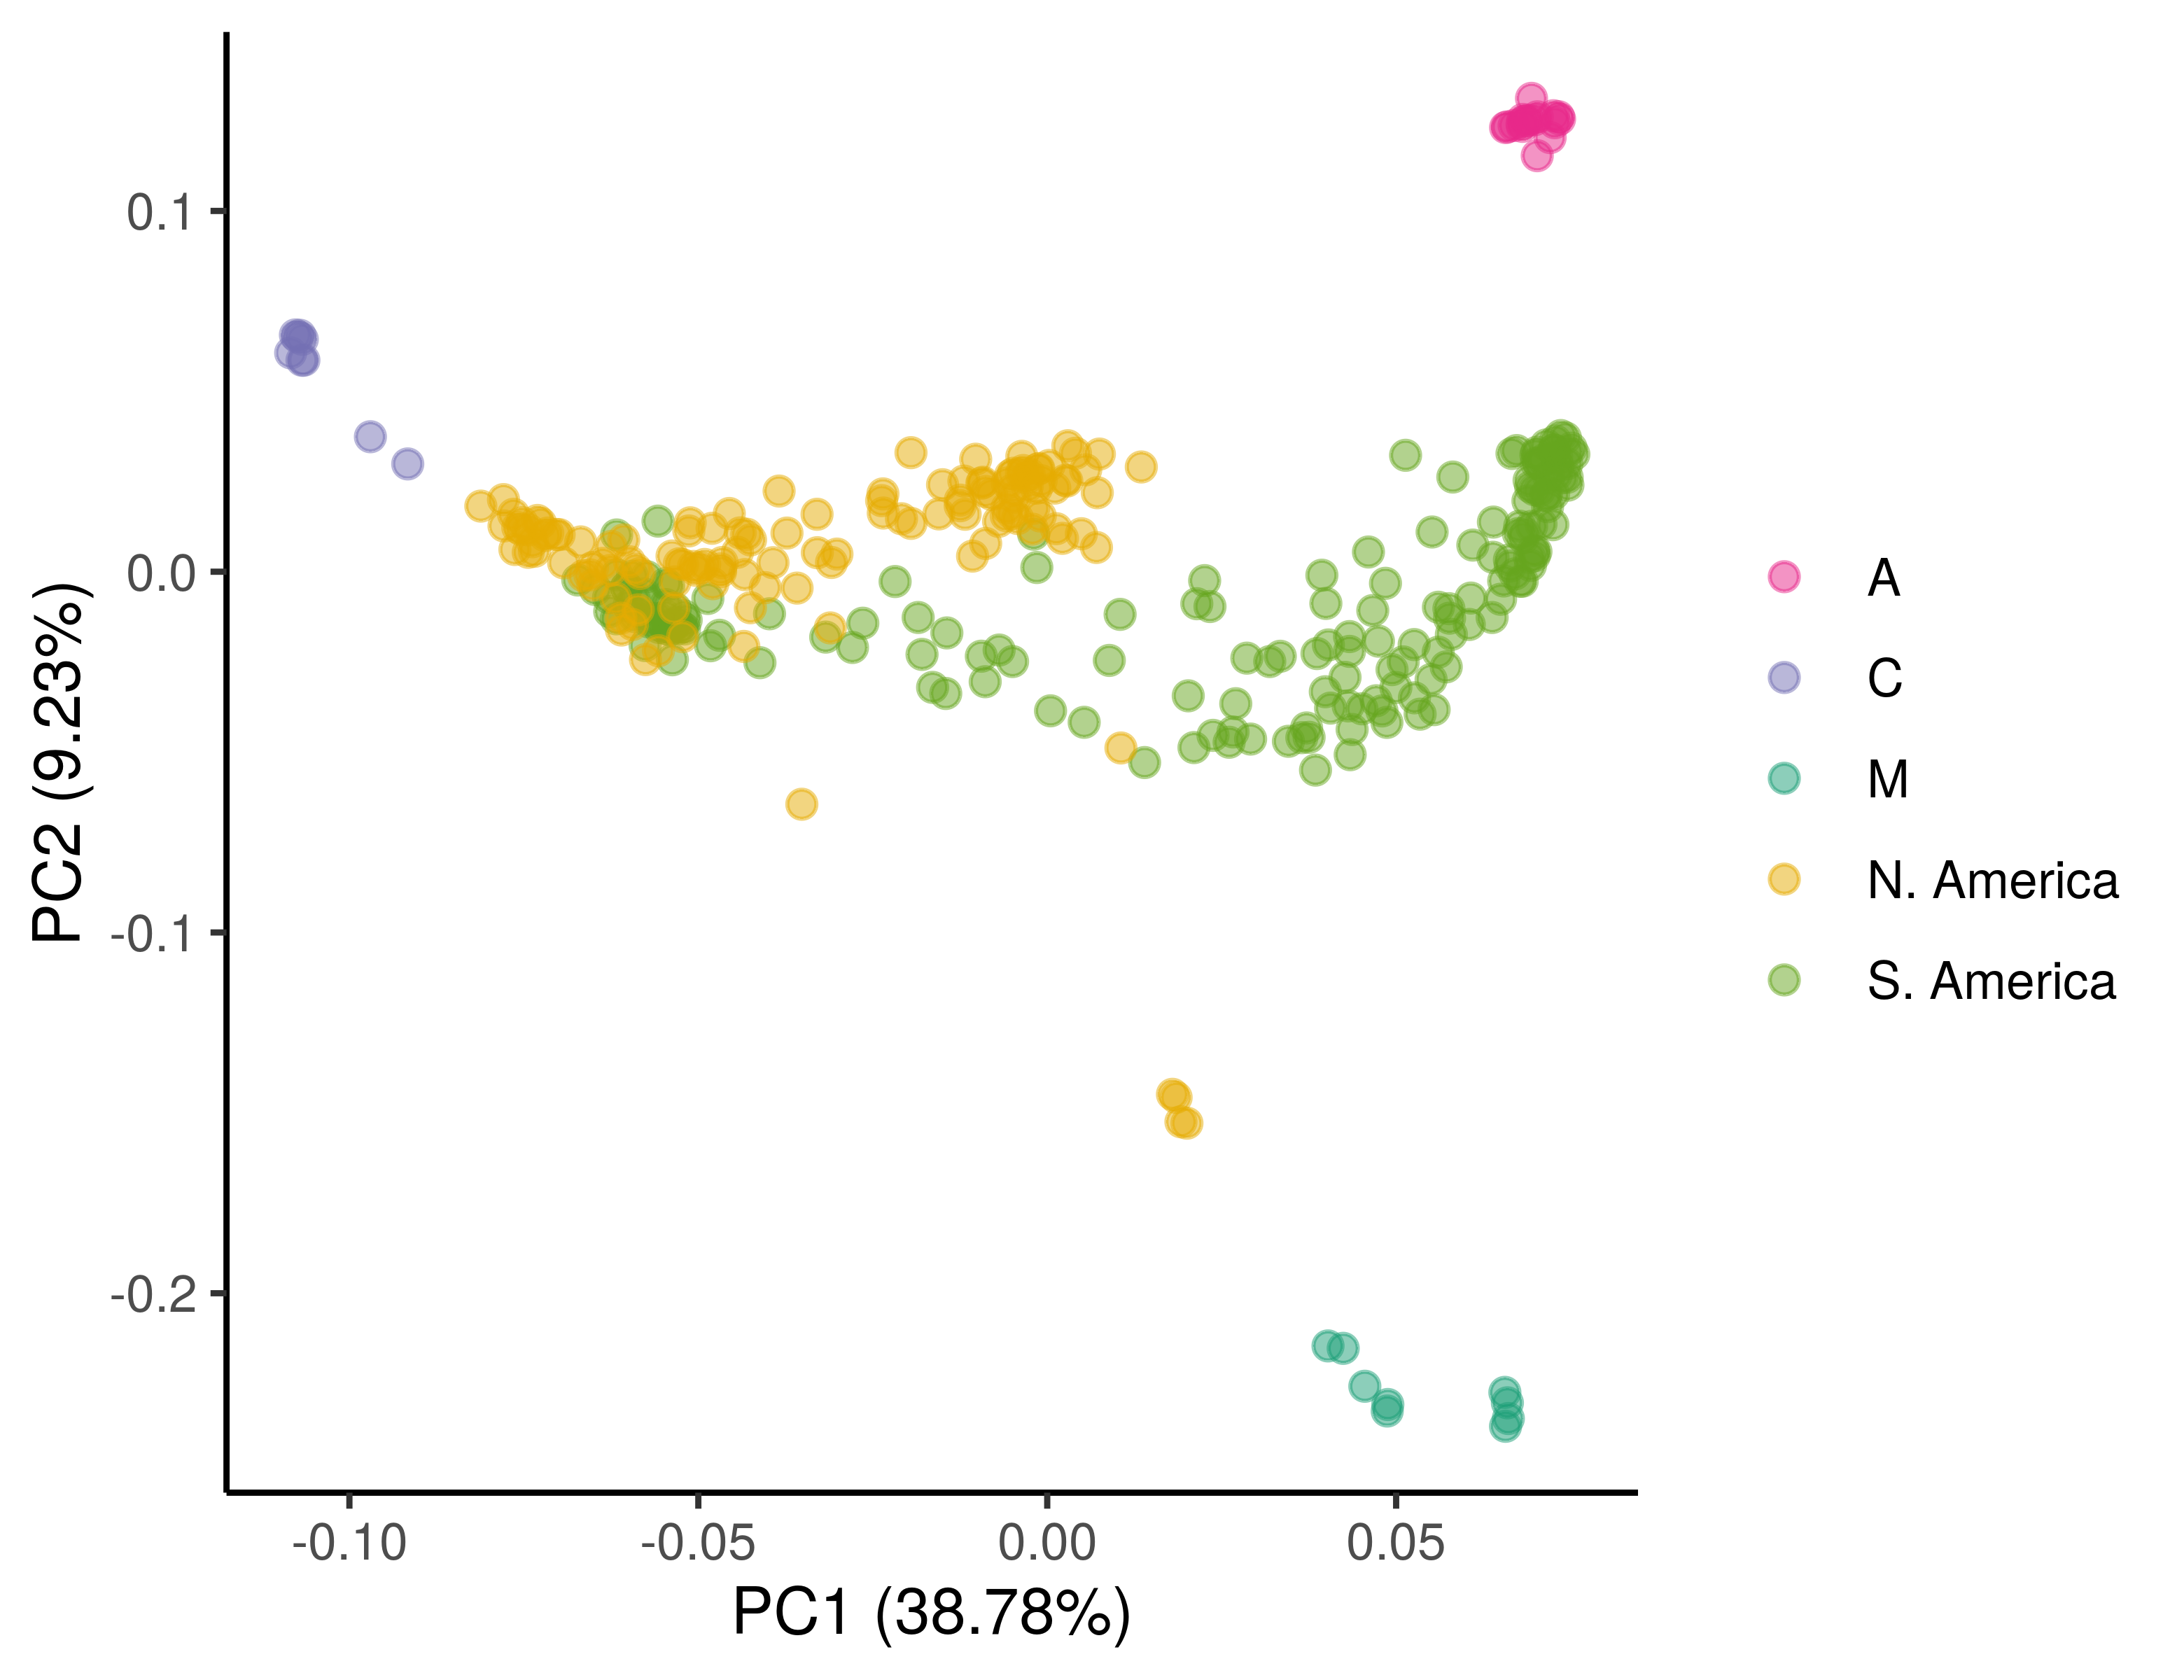
\includegraphics[width=\textwidth]{chapter1/figures/PCA_12_combined_sept19_byGroup.png}

\caption{ \textbf{PCA.} Principal components analysis generated in PCAngsd using genotype likelihoods from the same thinned set of 14,044 autosomal SNPs used in global admixture analysis. The major axes of diversity separate out C ancestry (PC1) and M ancestry (PC2). Consistent with 3-way admixture, all sampled bees from North and South America are intermediate on the PCA, in the triangle formed by reference panels for \ahb{\textit{Apis mellifera}} \scutellata\ \ahb{from southern and eastern Africa} (A), \ahb{\textit{A. m. carnica} from} eastern Europe (C) and \ahb{\textit{A. m. mellifera} and \textit{A. m. iberiensis} from} western Europe (M).}

\label{supp_pca}
\end{figure}

\begin{figure}[p]
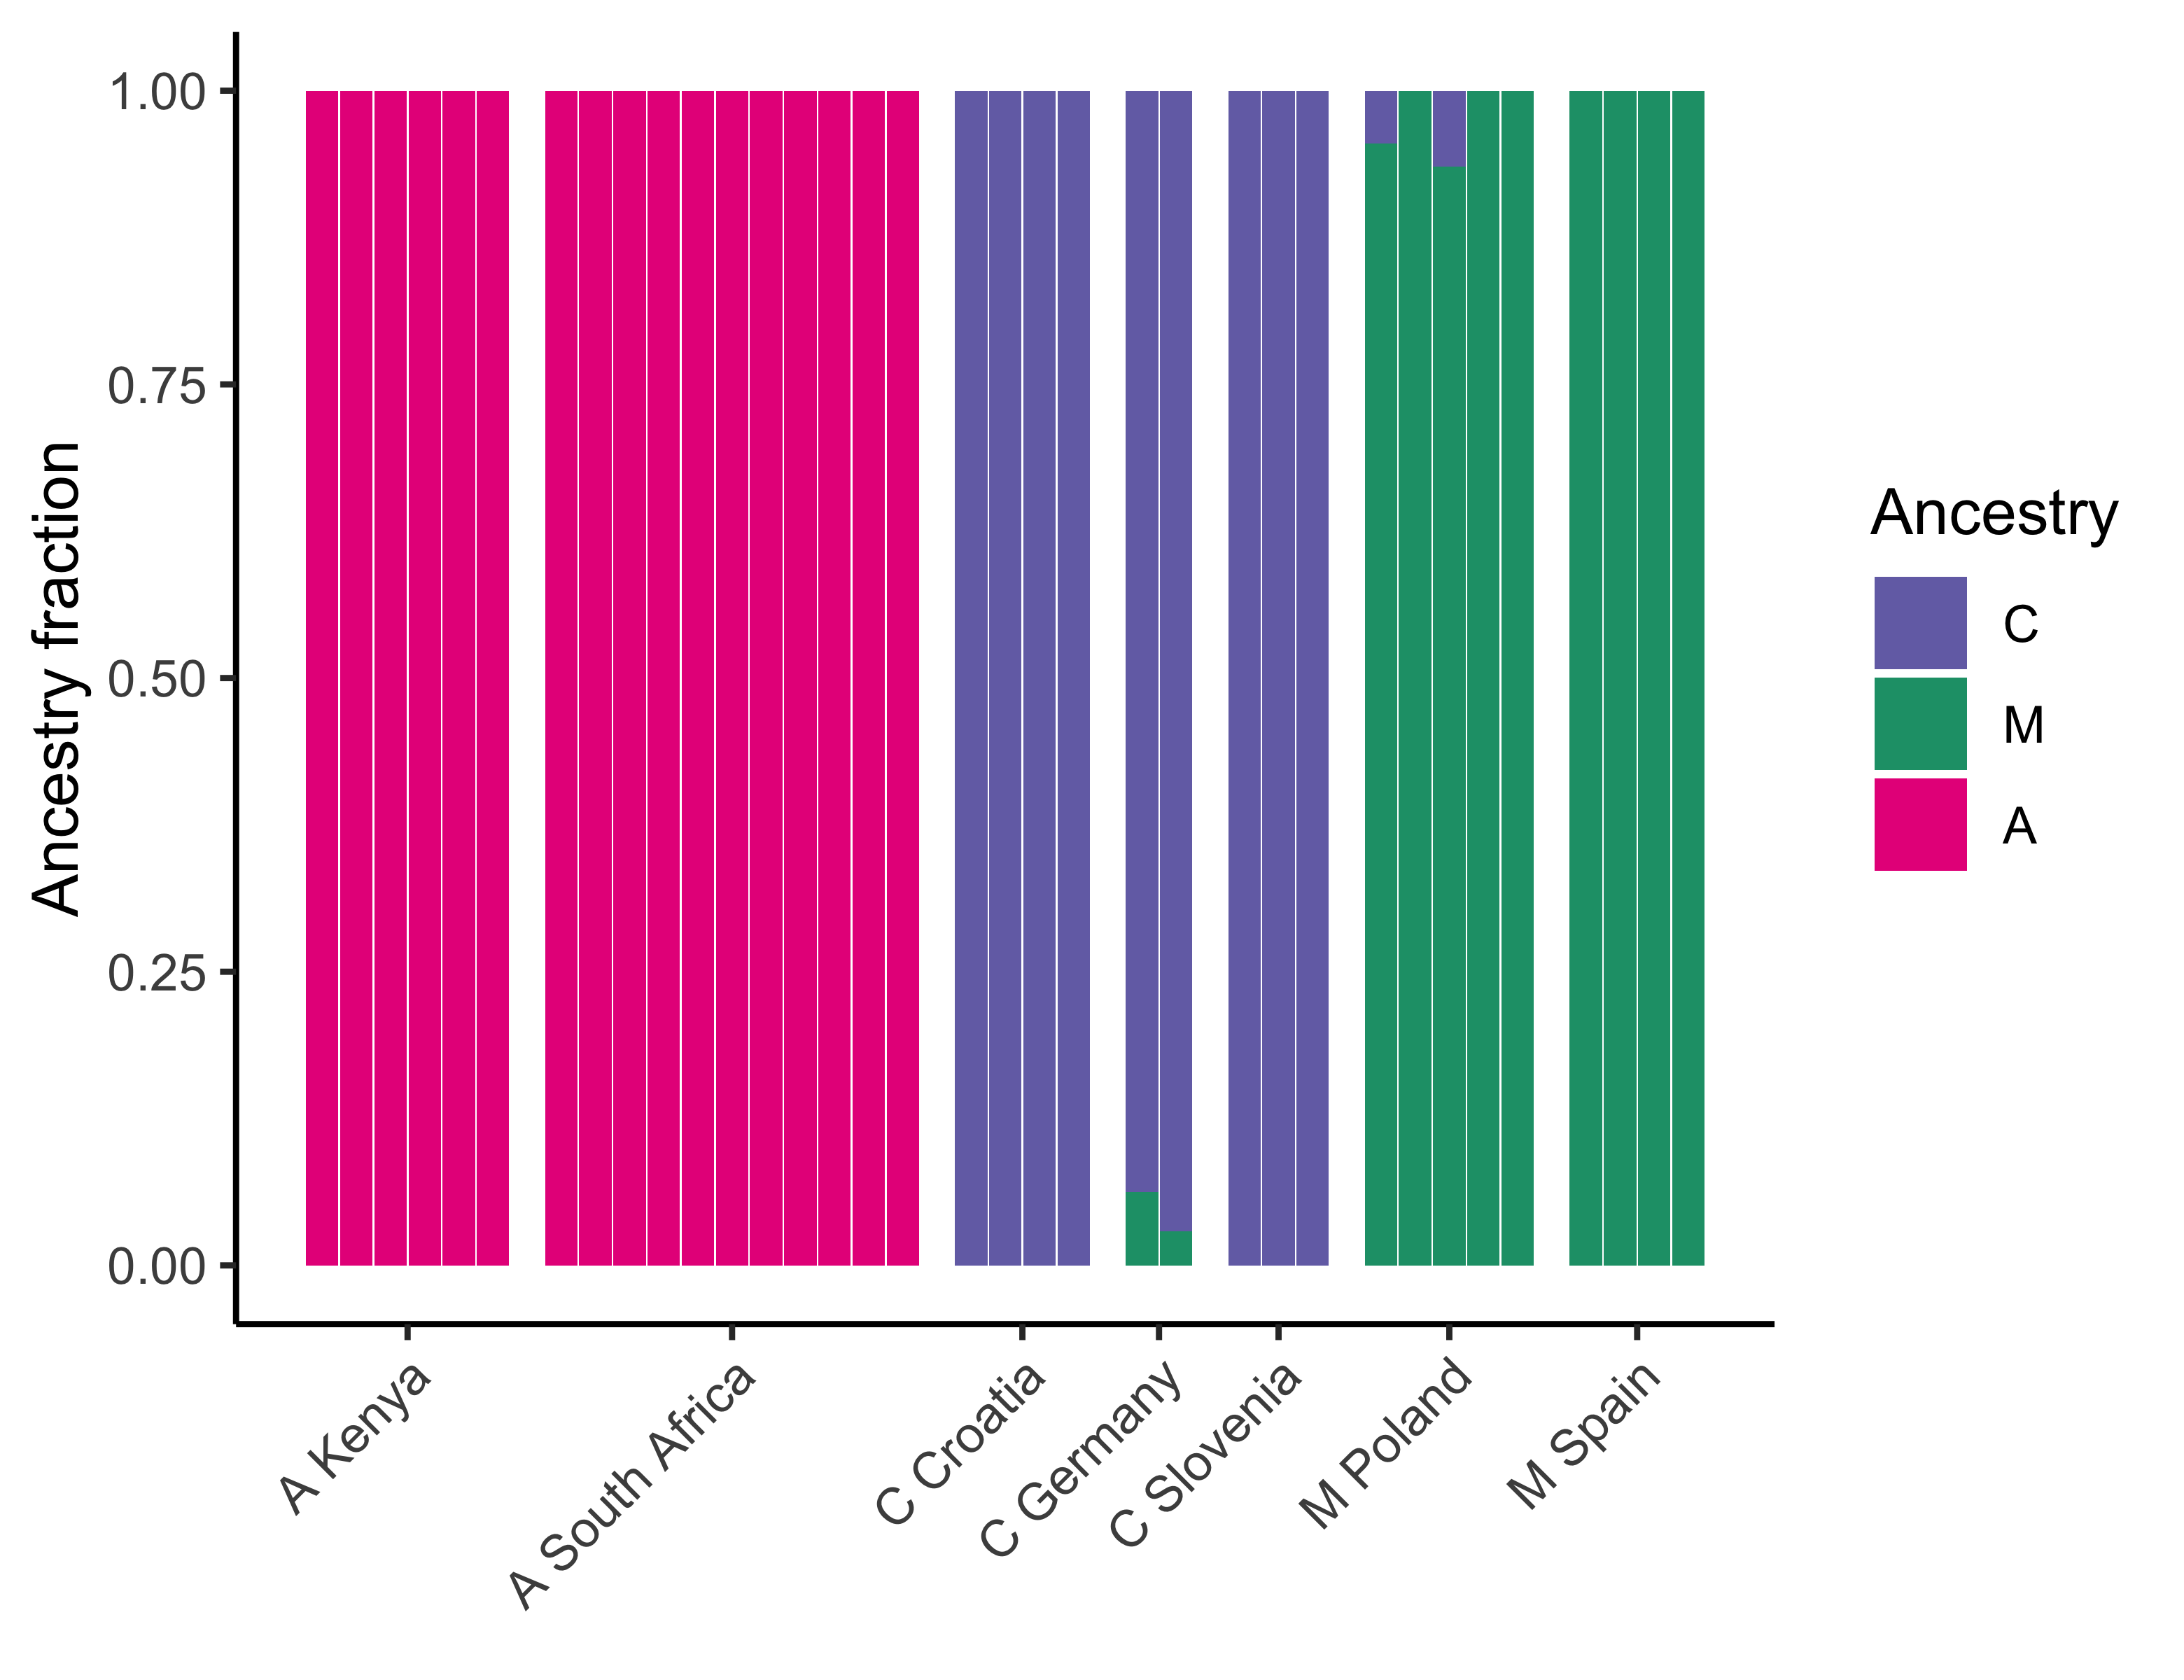
\includegraphics[width=\textwidth]{chapter1/figures/NGS_admix_refACM.png}
\caption{ \textbf{Ancestry in reference panels.} Results of NGSAdmix global admixture analysis for reference populations from the combined analysis of all populations (K = 3). These results were used to assign the unlabelled ancestry components output by NGSAdmix to A, C, and M groups, based on a clear mapping to the three reference populations. We see a small amount of admixture between C and M within our reference populations, which is consistent with limited gene flow from secondary contact within Europe.}

\label{ngsadmix_refACM}
\end{figure}

\begin{figure}[p]
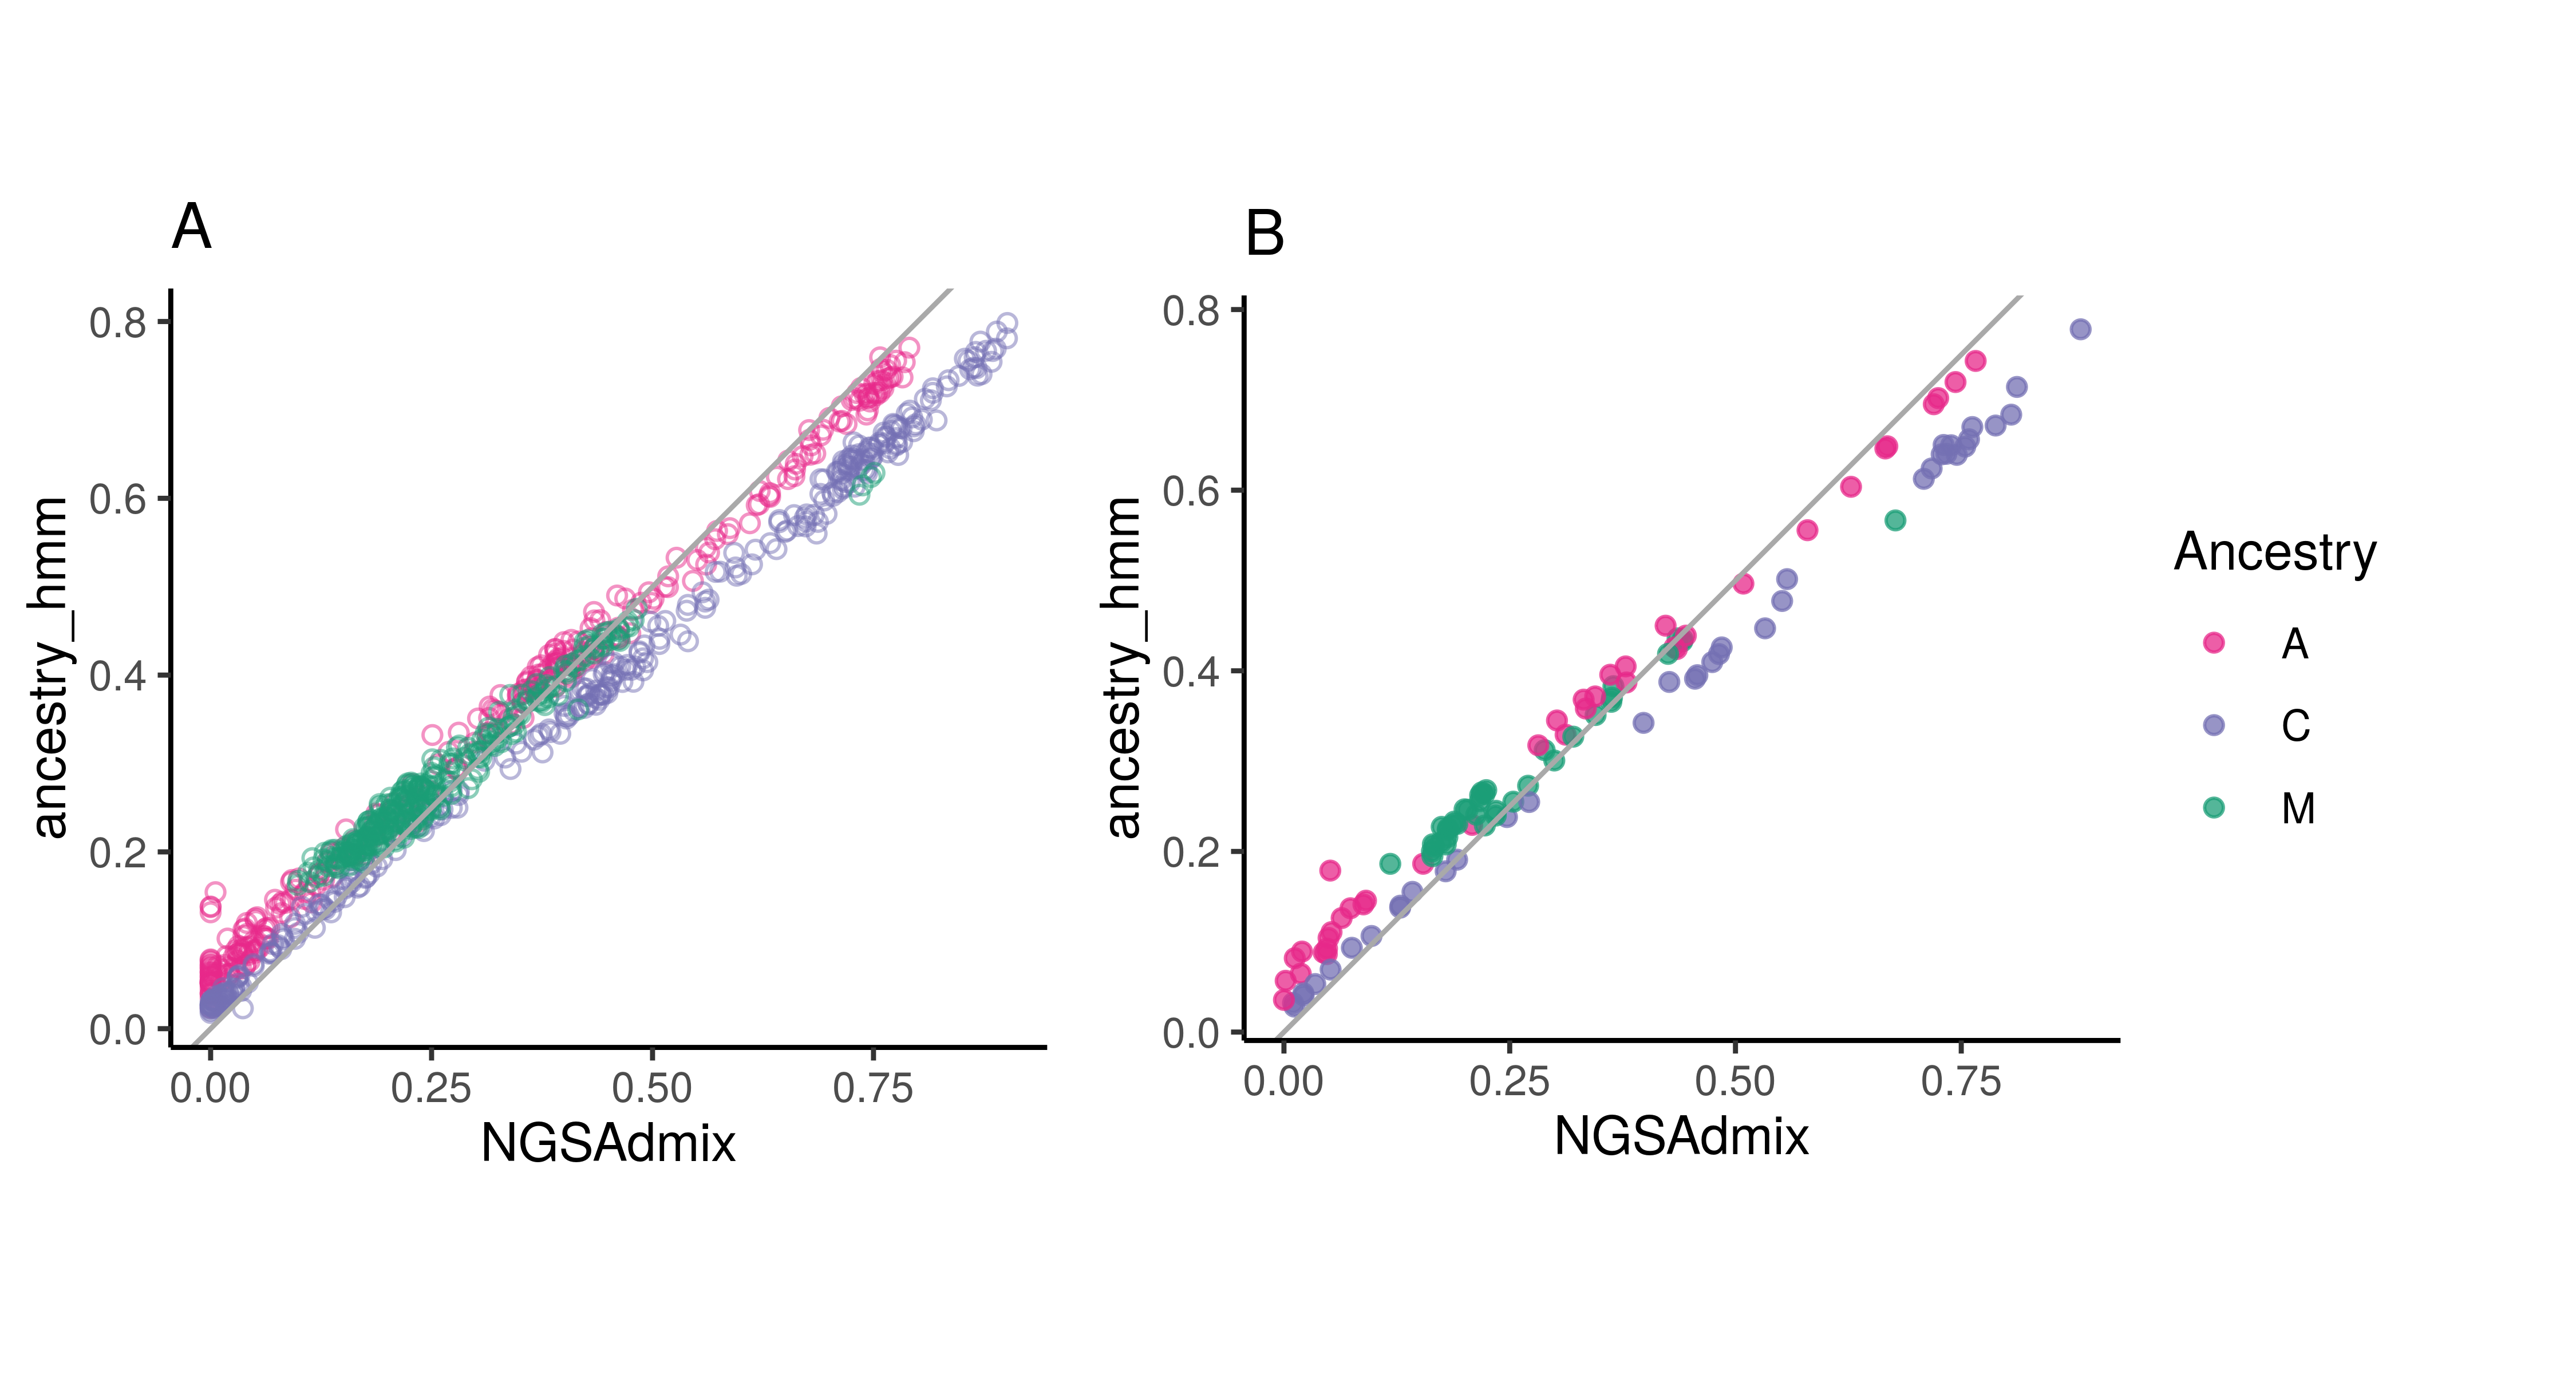
\includegraphics[width=\textwidth]{chapter1/figures/mean_ancestry_prior_posterior_ancestry_hmm.png}
\caption{ \textbf{Comparison of local and global ancestry results.} (A) Comparison of the mean genome-wide ancestry estimate from NGSAdmix (x-axis) and ancestry\_hmm (y-axis) for each bee, with one-to-one line drawn in grey. The mean for the HMM is calculated by marginalizing the posterior over all ancestry states and taking a mean across SNPs. The individual-level ancestry estimates between the two methods agree strongly (Pearson's correlation: 0.997 A, 0.999 C, 0.985 M), but the HMM estimates slightly higher minor ancestry for bees with low admixture proportions. (B) Population mean summarises for the same comparison of NGSAdmix vs. ancestry\_hmm genome-wide ancestry estimates, with one-to-one line drawn in gray. Because the population mean ancestry proportions from NGSAdmix are used as a prior for the population-specific mixing proportions in ancestry\_hmm, this panel can also be interpreted as the prior (x-axis) and posterior (y-axis) of the local ancestry HMM for population-level admixture proportions.}
\label{ngsadmix_vs_ancestry_hmm}
\end{figure}

\begin{figure}[ht]
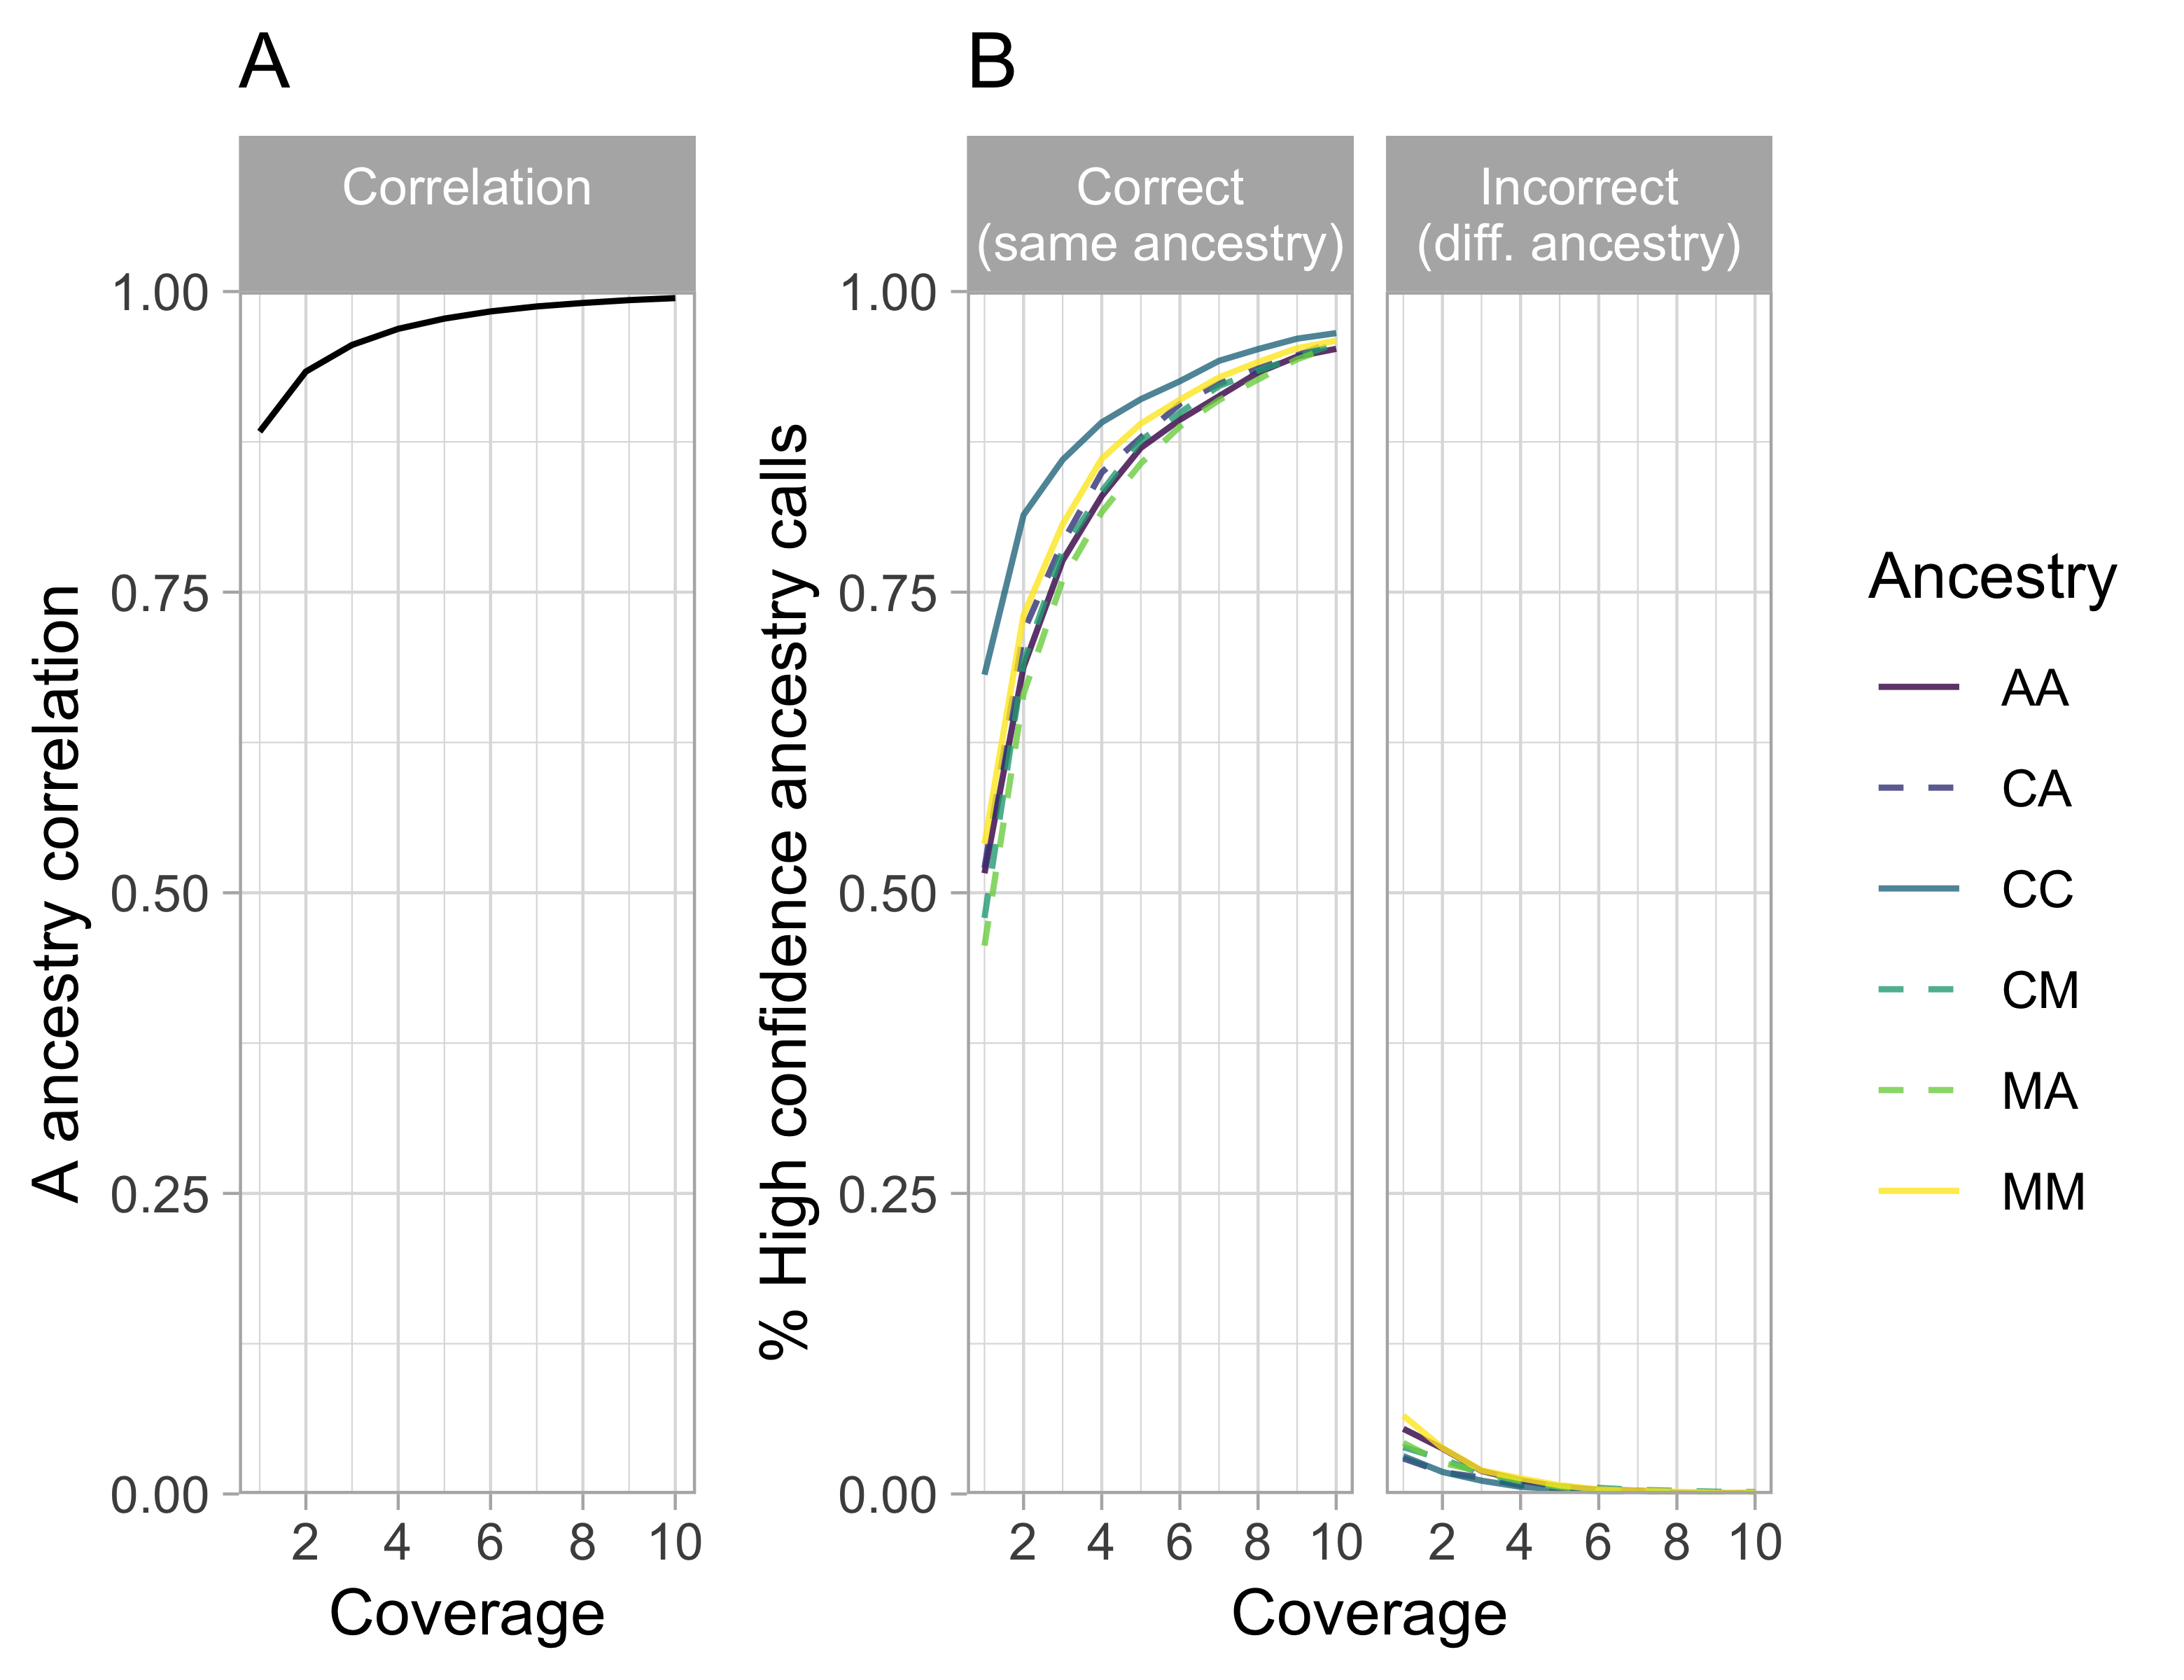
\includegraphics[width=.6\textwidth]{chapter1/figures/sims_downsample.png}
\caption{ \textbf{Power to call local ancestry.} (A) Correlation between high-coverage and low-coverage ancestry calls, across different simulated depths of coverage (1-10x). (B) Proportion of high-confidence ancestry calls from high-coverage data that were replicated in analyses of low-coverage data, with different simulated depths of coverage (1-10x). These results are from a preliminary analysis of the power to call local ancestry accurately, used to inform target sequencing depth for this study. For this preliminary study, we used a published SNP set with data for A, C, and M reference populations \cite{Cridland:2017el} based on earlier versions of the honey bee genome (Amel4.5 \cite{SequencingConsortium:2006ce}) and recombination map \cite{Wallberg:2014ha}. We enriched for ancestry-informativeness and thinned for linkage disequilibrium ($\geq 0.2$ MAF in at least one reference population and $r^2 < 0.4$ within the A reference population), leaving 161k SNPs. First we ran ancestry\_hmm \cite{CorbettDetig:2017gh} using called genotypes from a high-coverage admixed population with intermediate admixture proportions (Riverside 2014 (n=8): 40\% C, 20\% M, 40\% A ancestry). We simulated lower coverage data from this same population by generating a binomial sample of $n$ reads for each locus, based on the individual's genotype. To simulate realistic variance in coverage across the genome, $n$ for each site and individual was generated from a negative binomial distribution with variance 3x the mean \cite{Miller:2011en}. We additionally simulated a 1\% sequencing error rate. Running local ancestry inference on the high coverage data, we inferred high confidence ancestry states for 81\% of sites. First we calculated a point estimates for \A\  ancestry ($p(AA) + \nicefrac{1}{2}(p(CA) + p(MA))$) at every site for each individual and used these estimates to calculate a correlation between the high coverage ancestry calls and low coverage ancestry calls. Then we calculated the percent of high confidence calls that were replicated with high confidence (\textgreater 0.8 posterior) in the low coverage data for the same ancestry state ("correct") or a different ancestry state ("incorrect"). Call to the HMM for simulated low-coverage data: ancestry\_hmm -e 3e-3 -a 3 0.4 0.2 0.4 -p 0 100000 0.4 -p 1 -100 0.2 -p 2 -60 0.4 --tmax 150 --tmin 2 --ne 670000. For original high coverage data we used genotype calls rather than read counts (-g) and a lower error rate (-e 1e-3).}

\label{sims_downsample}
\end{figure}

\begin{figure}[ht]
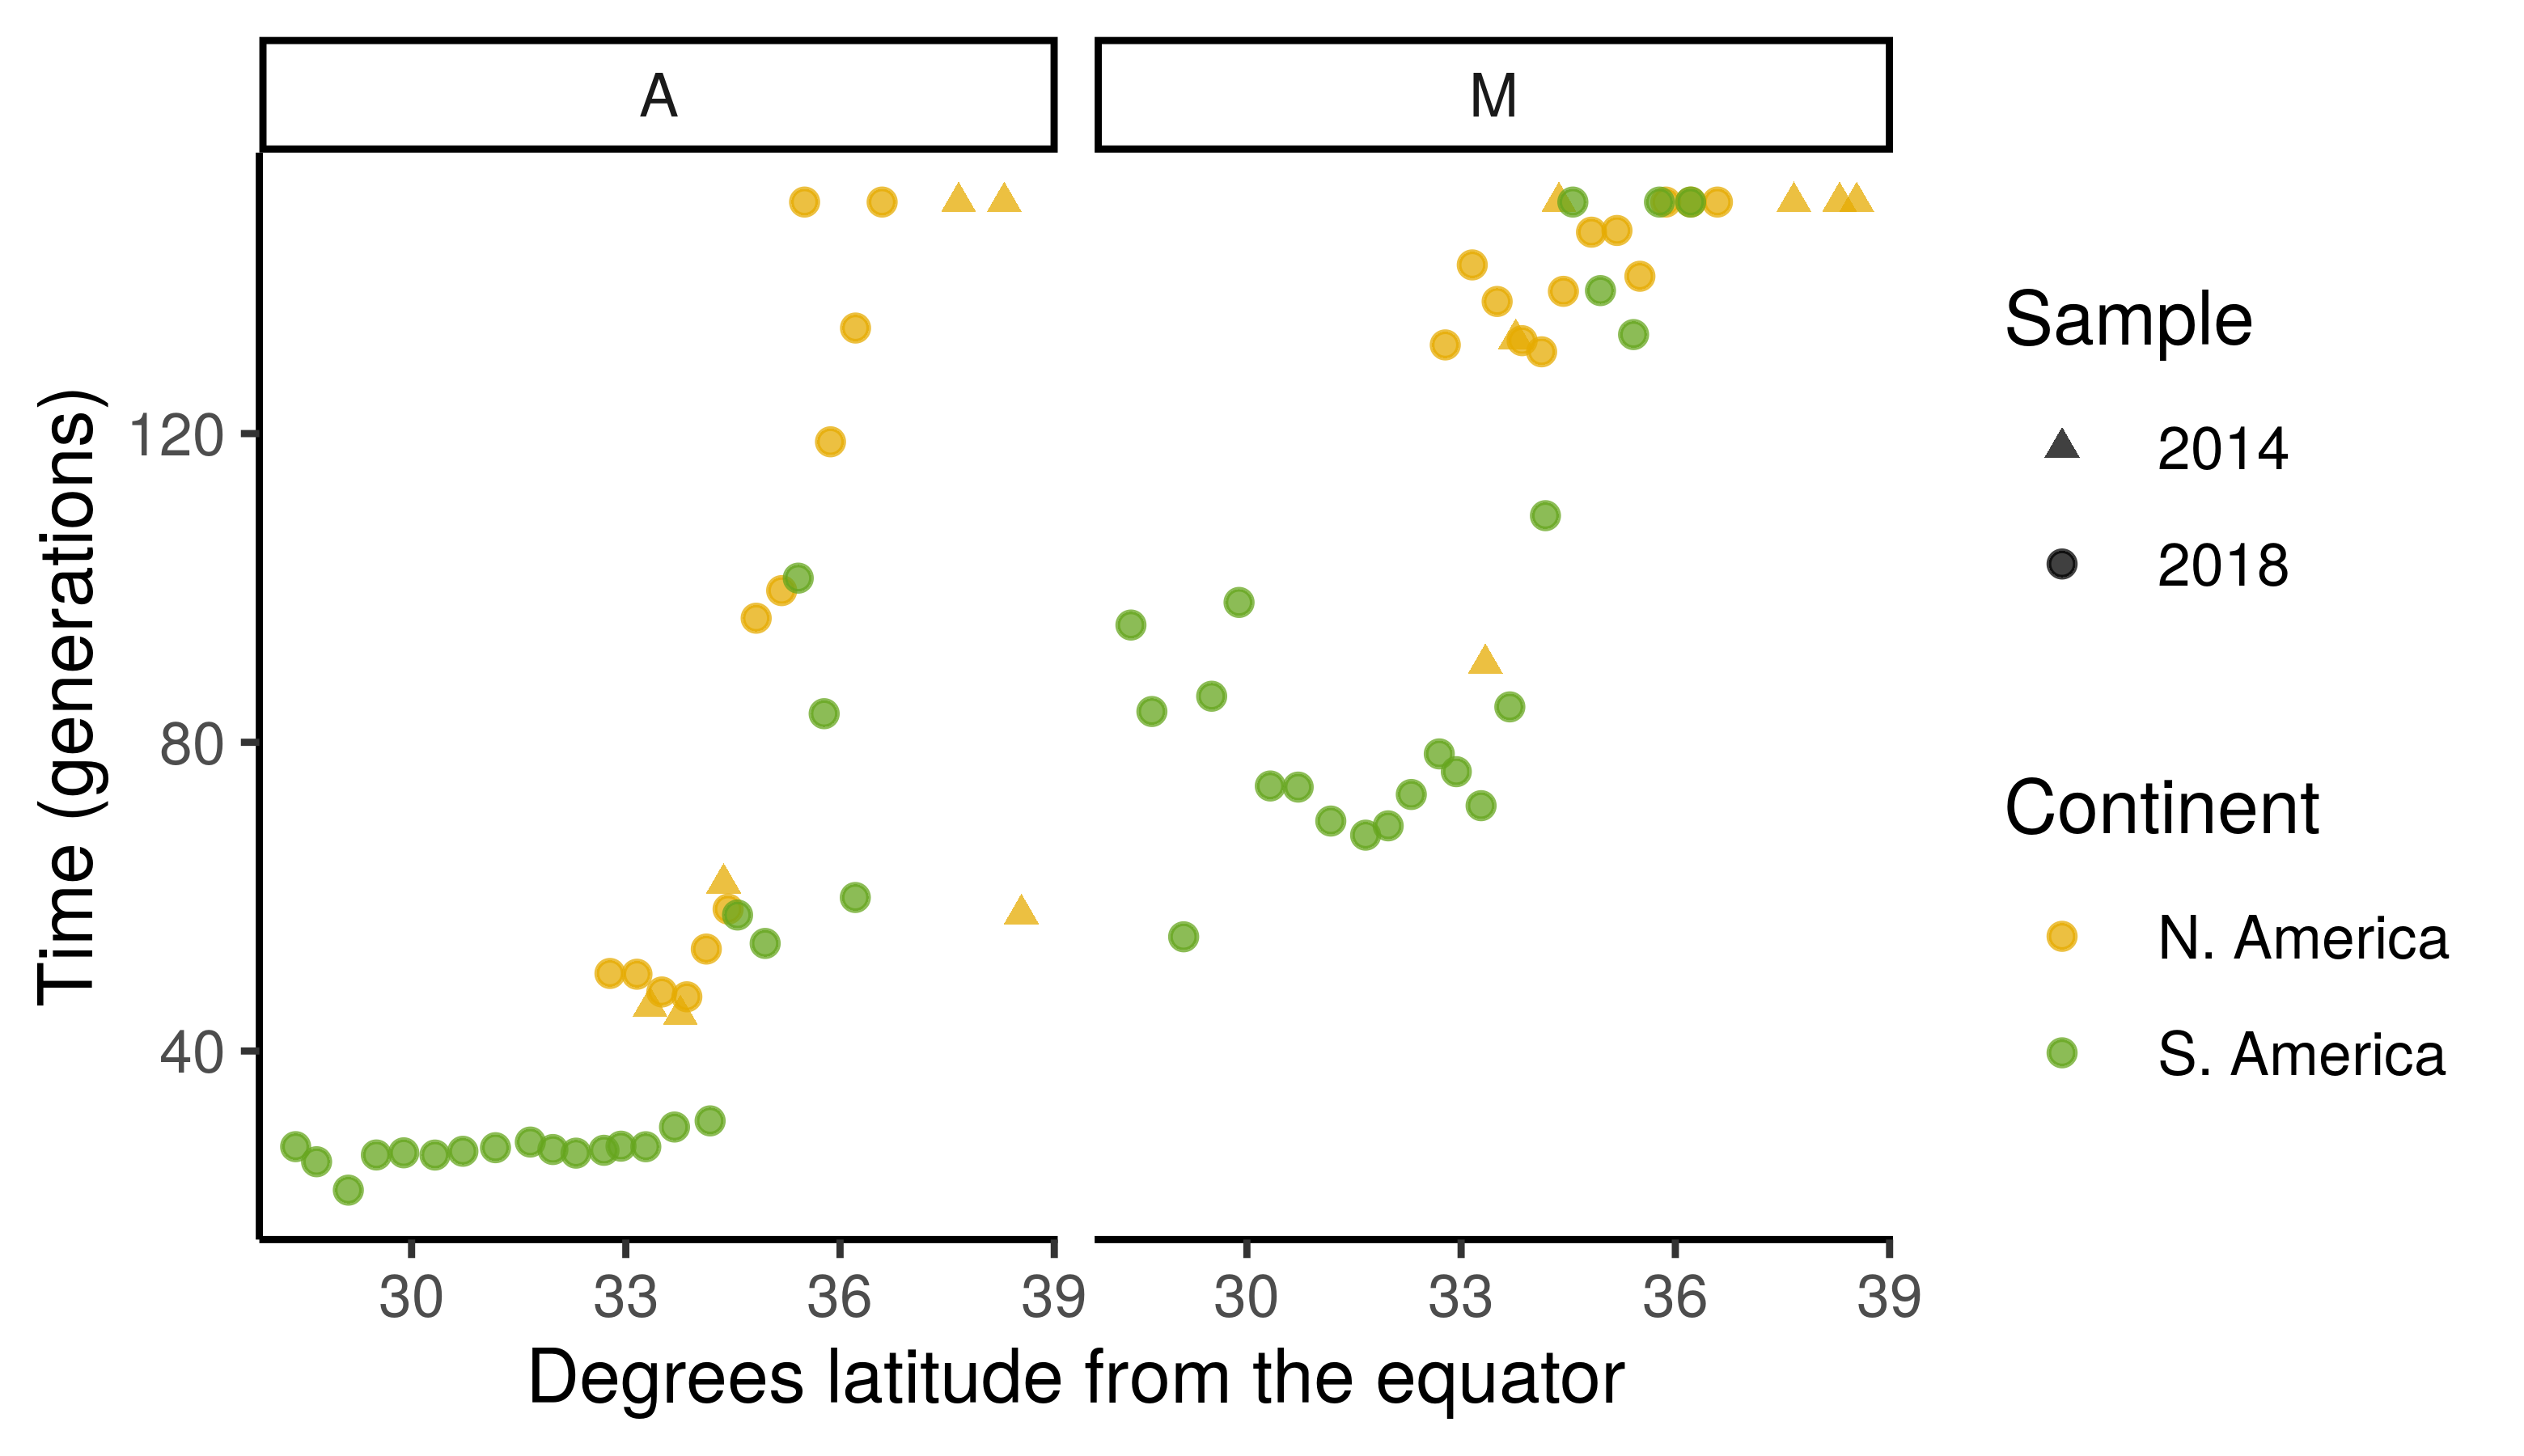
\includegraphics[width=\textwidth]{chapter1/figures/time_of_admixture_vs_latitude.png}

\caption{ \textbf{Estimated generations post-admixture.} Inferred timing of migration pulses from A ancestry (left) and M ancestry (right). Each population's admixture timing is estimated separately, during local ancestry inference (ancestry\_hmm), and results are plotted across latitude. We allowed a range of 2-150 generations, so the highest time estimates are truncated at 150 generations. Admixture with \scutellata\ (A) ancestry began in 1956, 62 years before sampling in 2018. We have little prior information about the timing of M into C admixture, which likely varies across the Americas, but in general should pre-date \ahb{admixture with A}. The number of generations per year for feral honey bee populations is uncertain.}
\label{supp_time_admixture}
\end{figure}

\begin{figure}[ht]
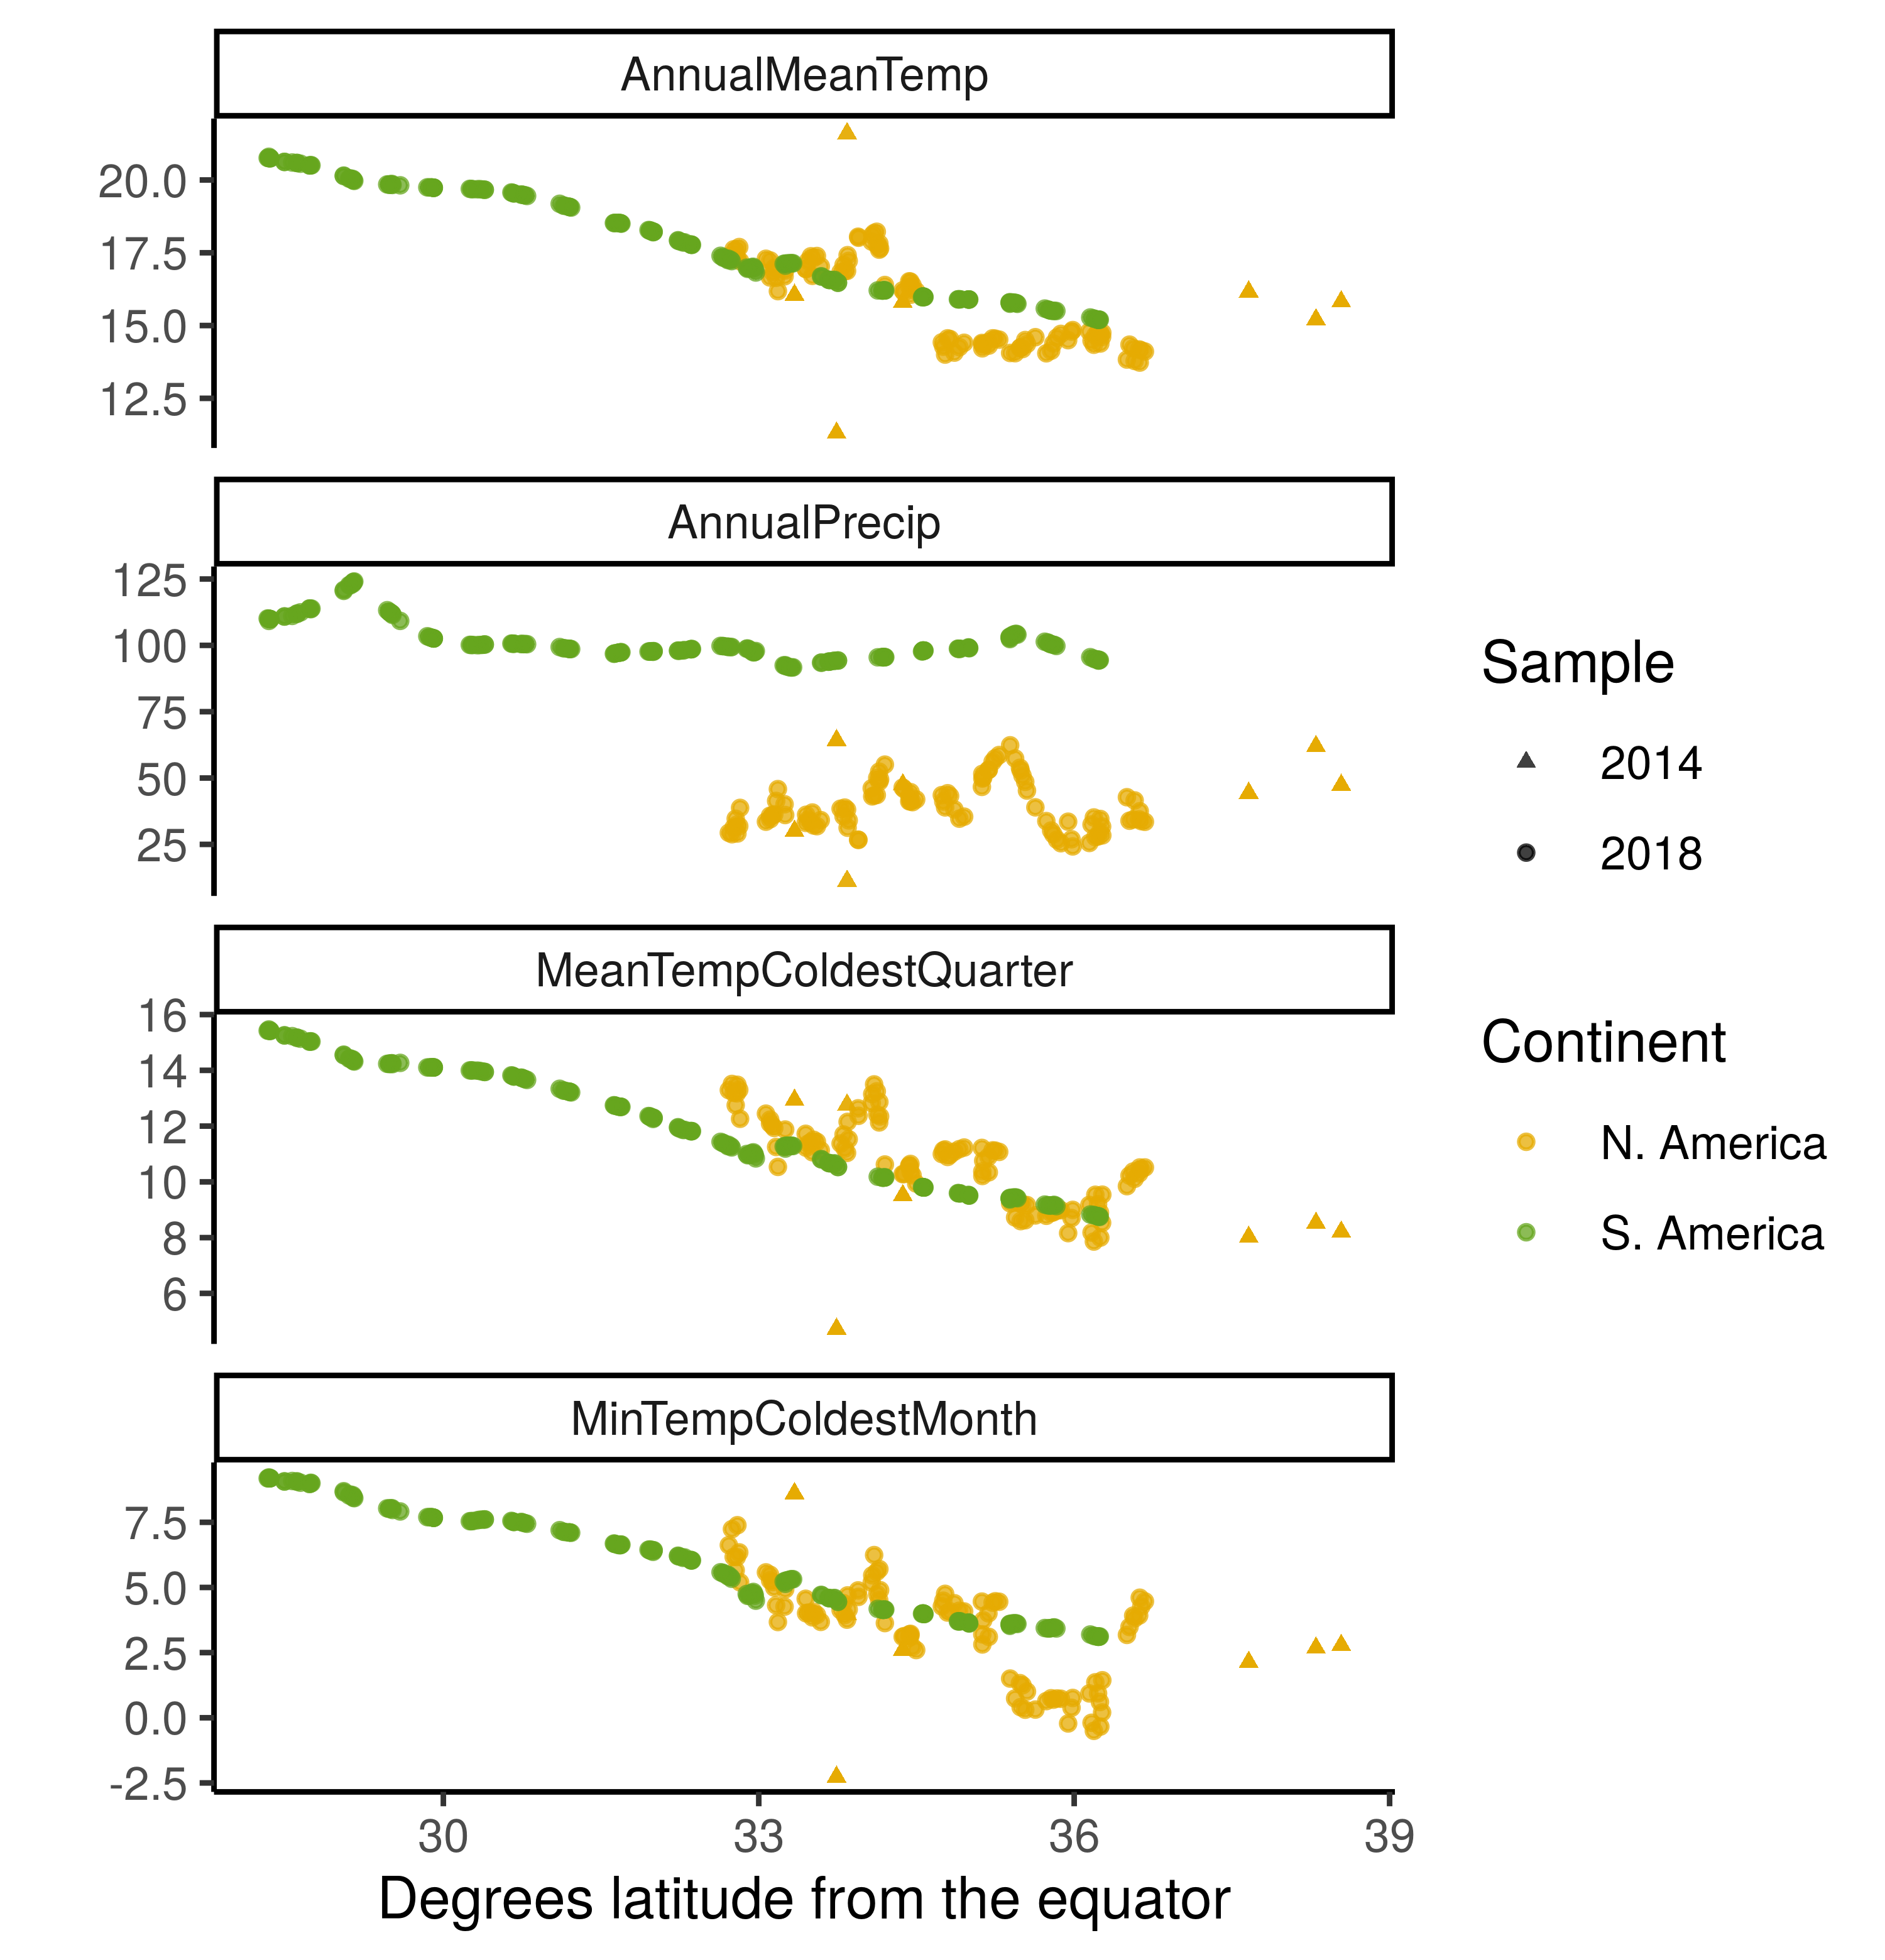
\includegraphics[width=.9\textwidth]{chapter1/figures/climate_variables_across_latitude.png}
\caption{ \textbf{Climate variables across latitude.} Bioclim climate variables for all sample sites plotted against latitude: (A) Mean annual temperature (B) Mean annual precipitation (C) Mean temperature coldest quarter (D) Minimum temperature coldest month. Two adjacent climate outliers in the N. American sample can be seen in the top two panels and represent bees from an inland desert (hot and dry) and a high altitude sampling site (cold and wet) at similar latitudes in Riverside County, CA. Bees from this same high altitude site are also outliers in the bottom two panels, having the coldest mean and minimum winter temperatures of all sites.}

\label{supp_bioclim}
\end{figure}

\begin{figure}[ht]
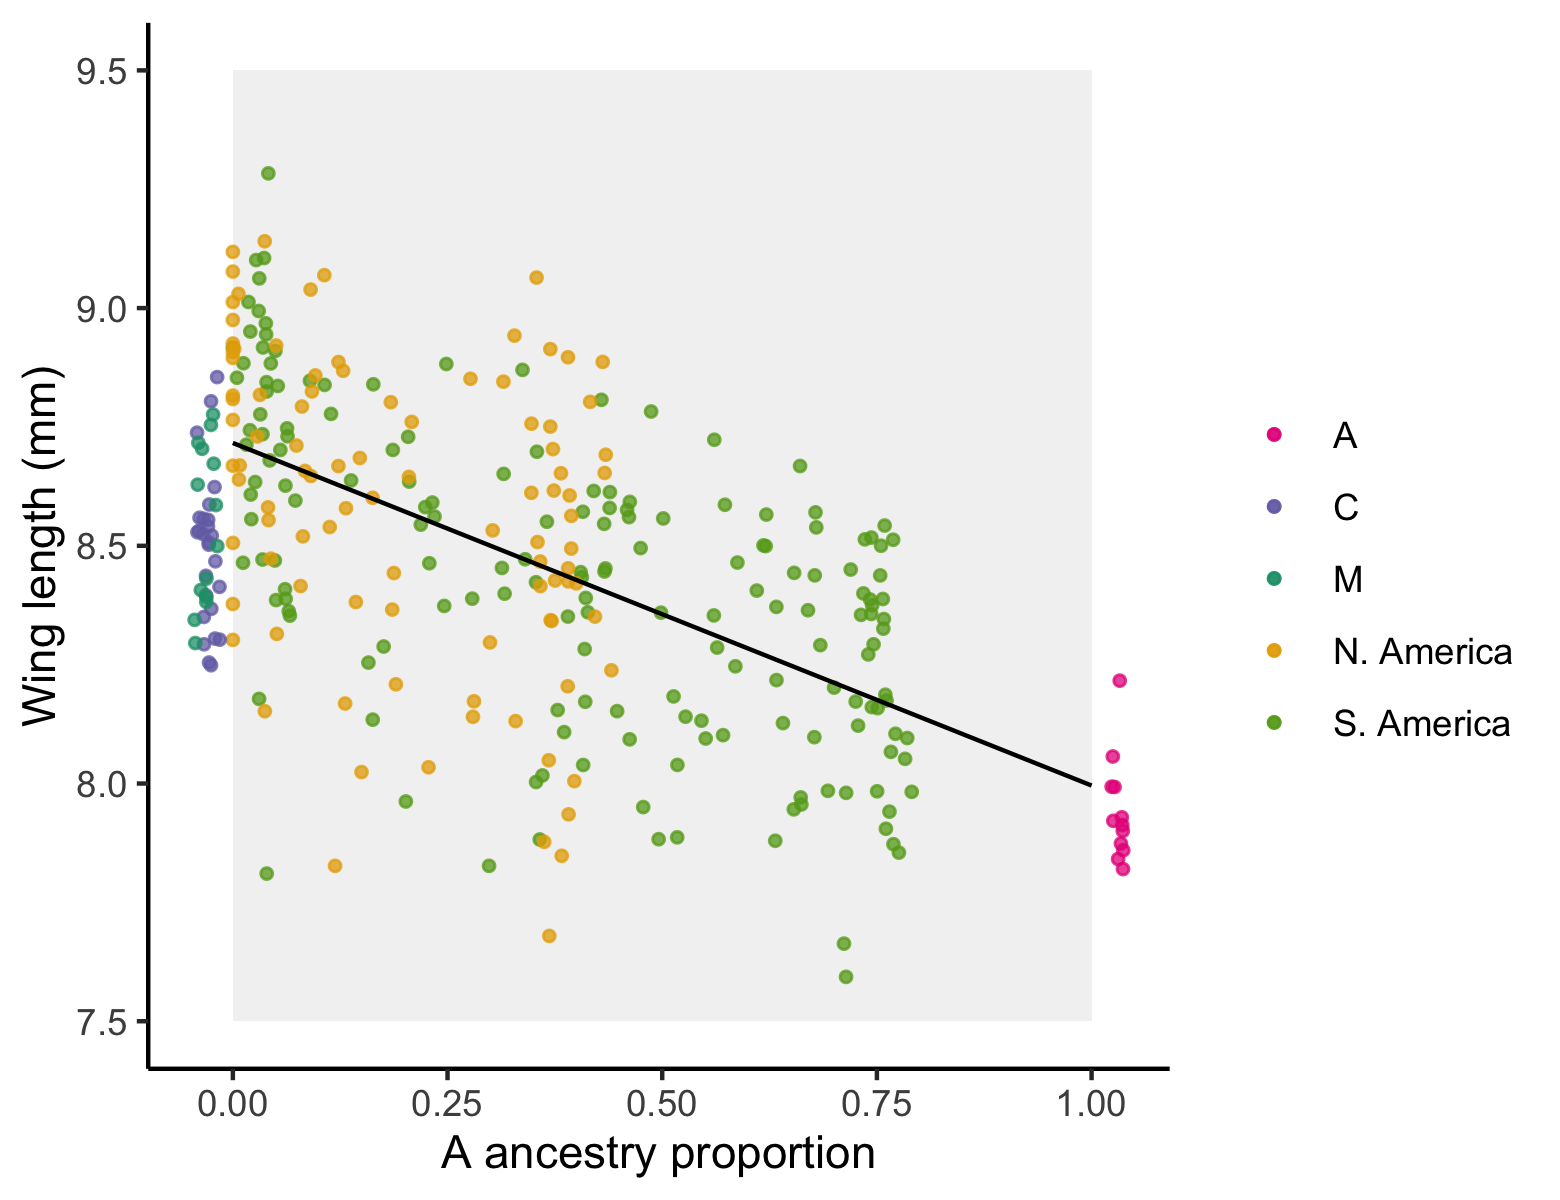
\includegraphics[width=\textwidth]{chapter1/figures/wing_length_by_A_ancestry.png}
\caption{ \textbf{Wing length predicted by ancestry.} Individual honey bees are represented as points, with wing lengths plotted along the x-axis and genomewide \A\ ancestry proportions (NGSAdmix results) along the y-axis. We draw the best-fit regression line (slope = -0.72 mm, $F(1, 267) = 119$, $P = 3.65\times10^{-23}$, $R^{2} = 0.31$, $n = 269$). We also include wing lengths for \ahb{A, C and M} reference bees from the Oberursel Collection, which we assume have none or full A ancestry. These reference bees are plotted slightly outside the range [0,1] and with jitter to facilitate viewing individual points that would otherwise all cluster on the boundaries.}
\label{wing_length_by_A_ancestry}
\end{figure}

\begin{figure}[ht]
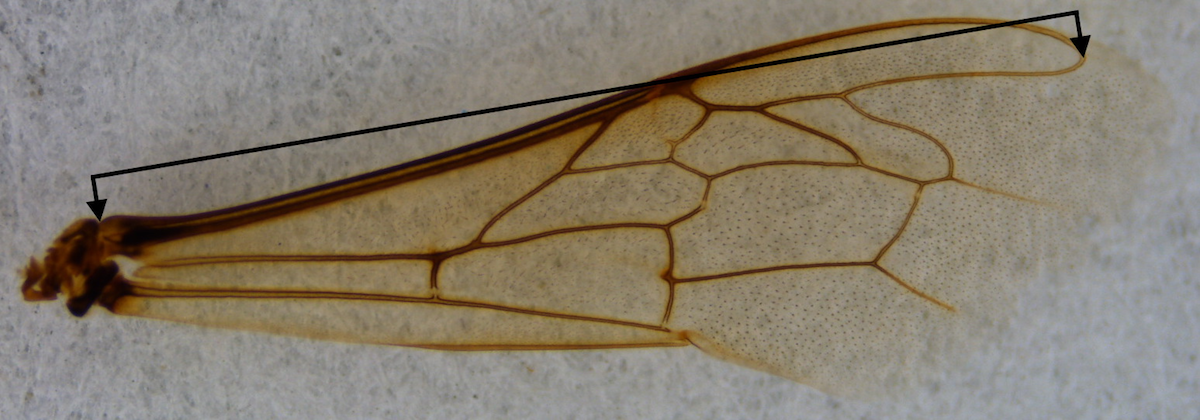
\includegraphics{chapter1/figures/wing_length_measurement.png}
\caption{ \textbf{Wing length measurement}. Fore wing image cropped and annotated to show length measurement taken. A full length to the tip of the wing is the standard measurement, but we use this alternative because many of our samples have significant wing tatter.}
\label{wing_image}
\end{figure}

\begin{figure}[ht]
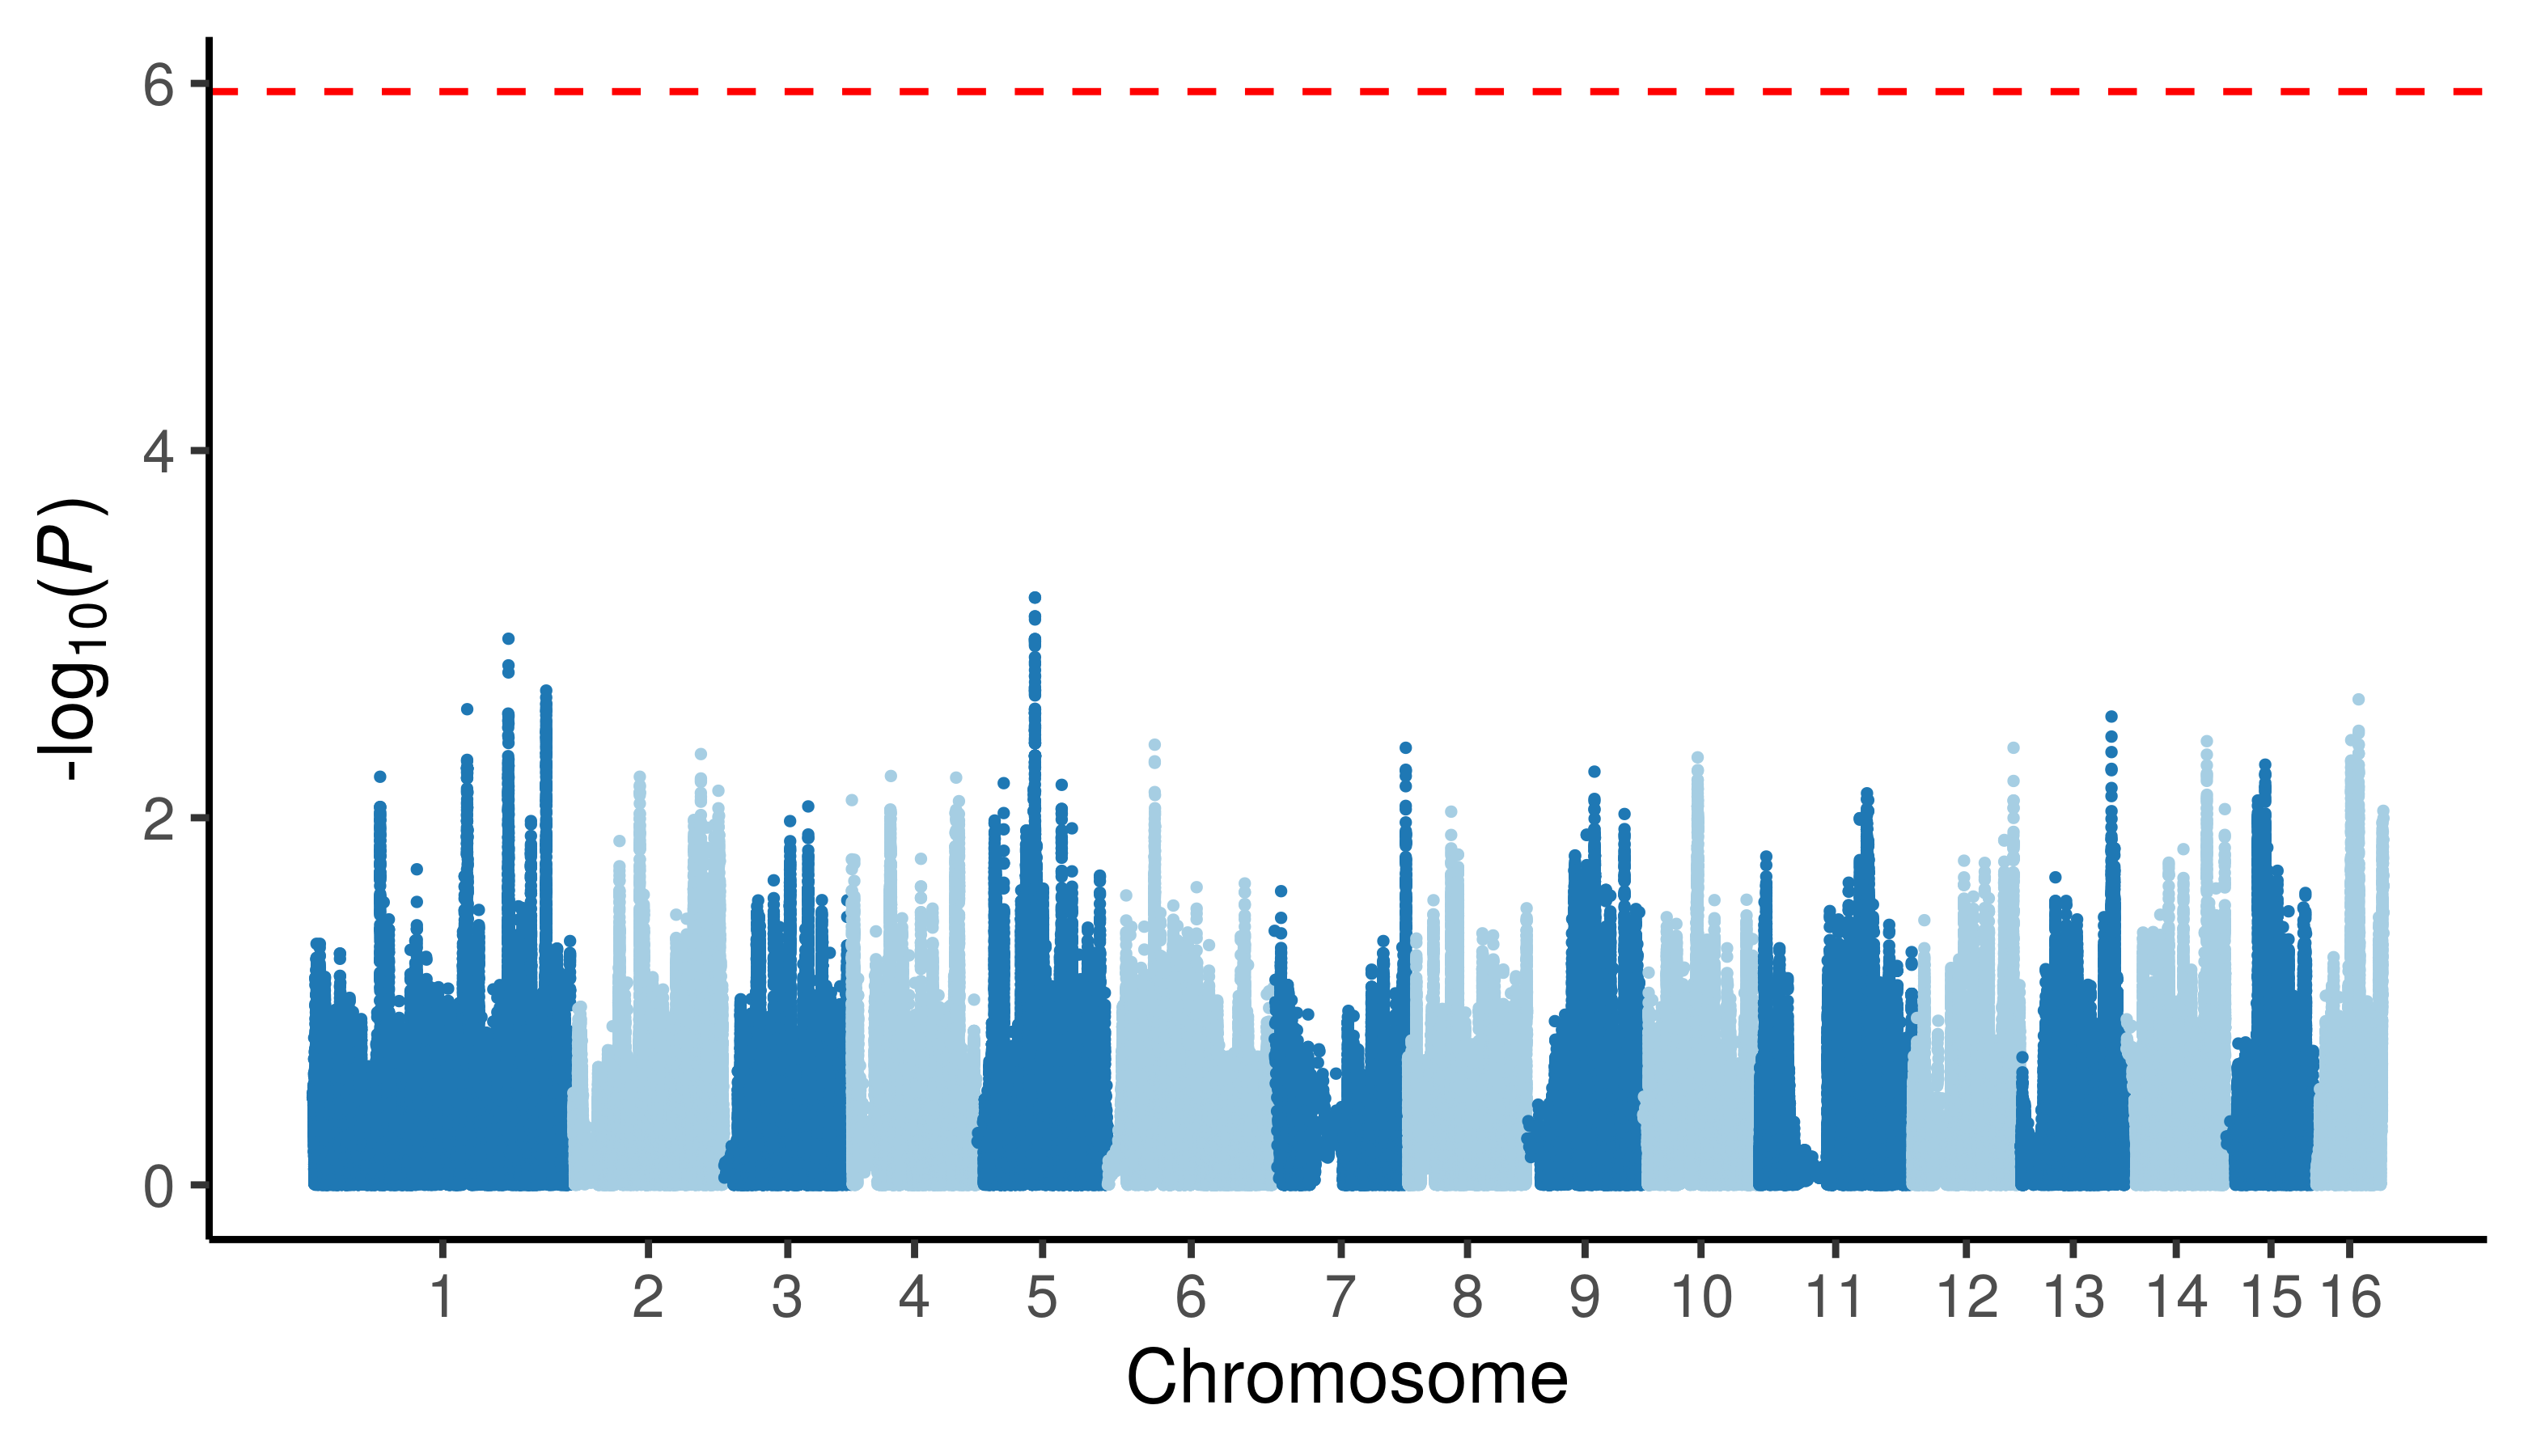
\includegraphics[width=\textwidth]{chapter1/figures/admixture_mapping_wing_length.png}
\caption{ \textbf{Admixture mapping analysis.} We plot the p-value for each SNP across the genome, based on independent tests of association between \A\ ancestry at that SNP and wing length. The red dashed line marks the genome-wide significance threshold for a family-wise error rate of 0.05, using a two-tailed test. In admixture mapping, SNPs are correlated, and the number of independent statistical tests depends on the number of generations recombination has had to break up ancestry blocks. Here we use an analytical approximation for the significance threshold based on 47.65 generations of admixture (population median estimate).}
\label{admixture_mapping}
\end{figure}


\begin{figure}[ht]
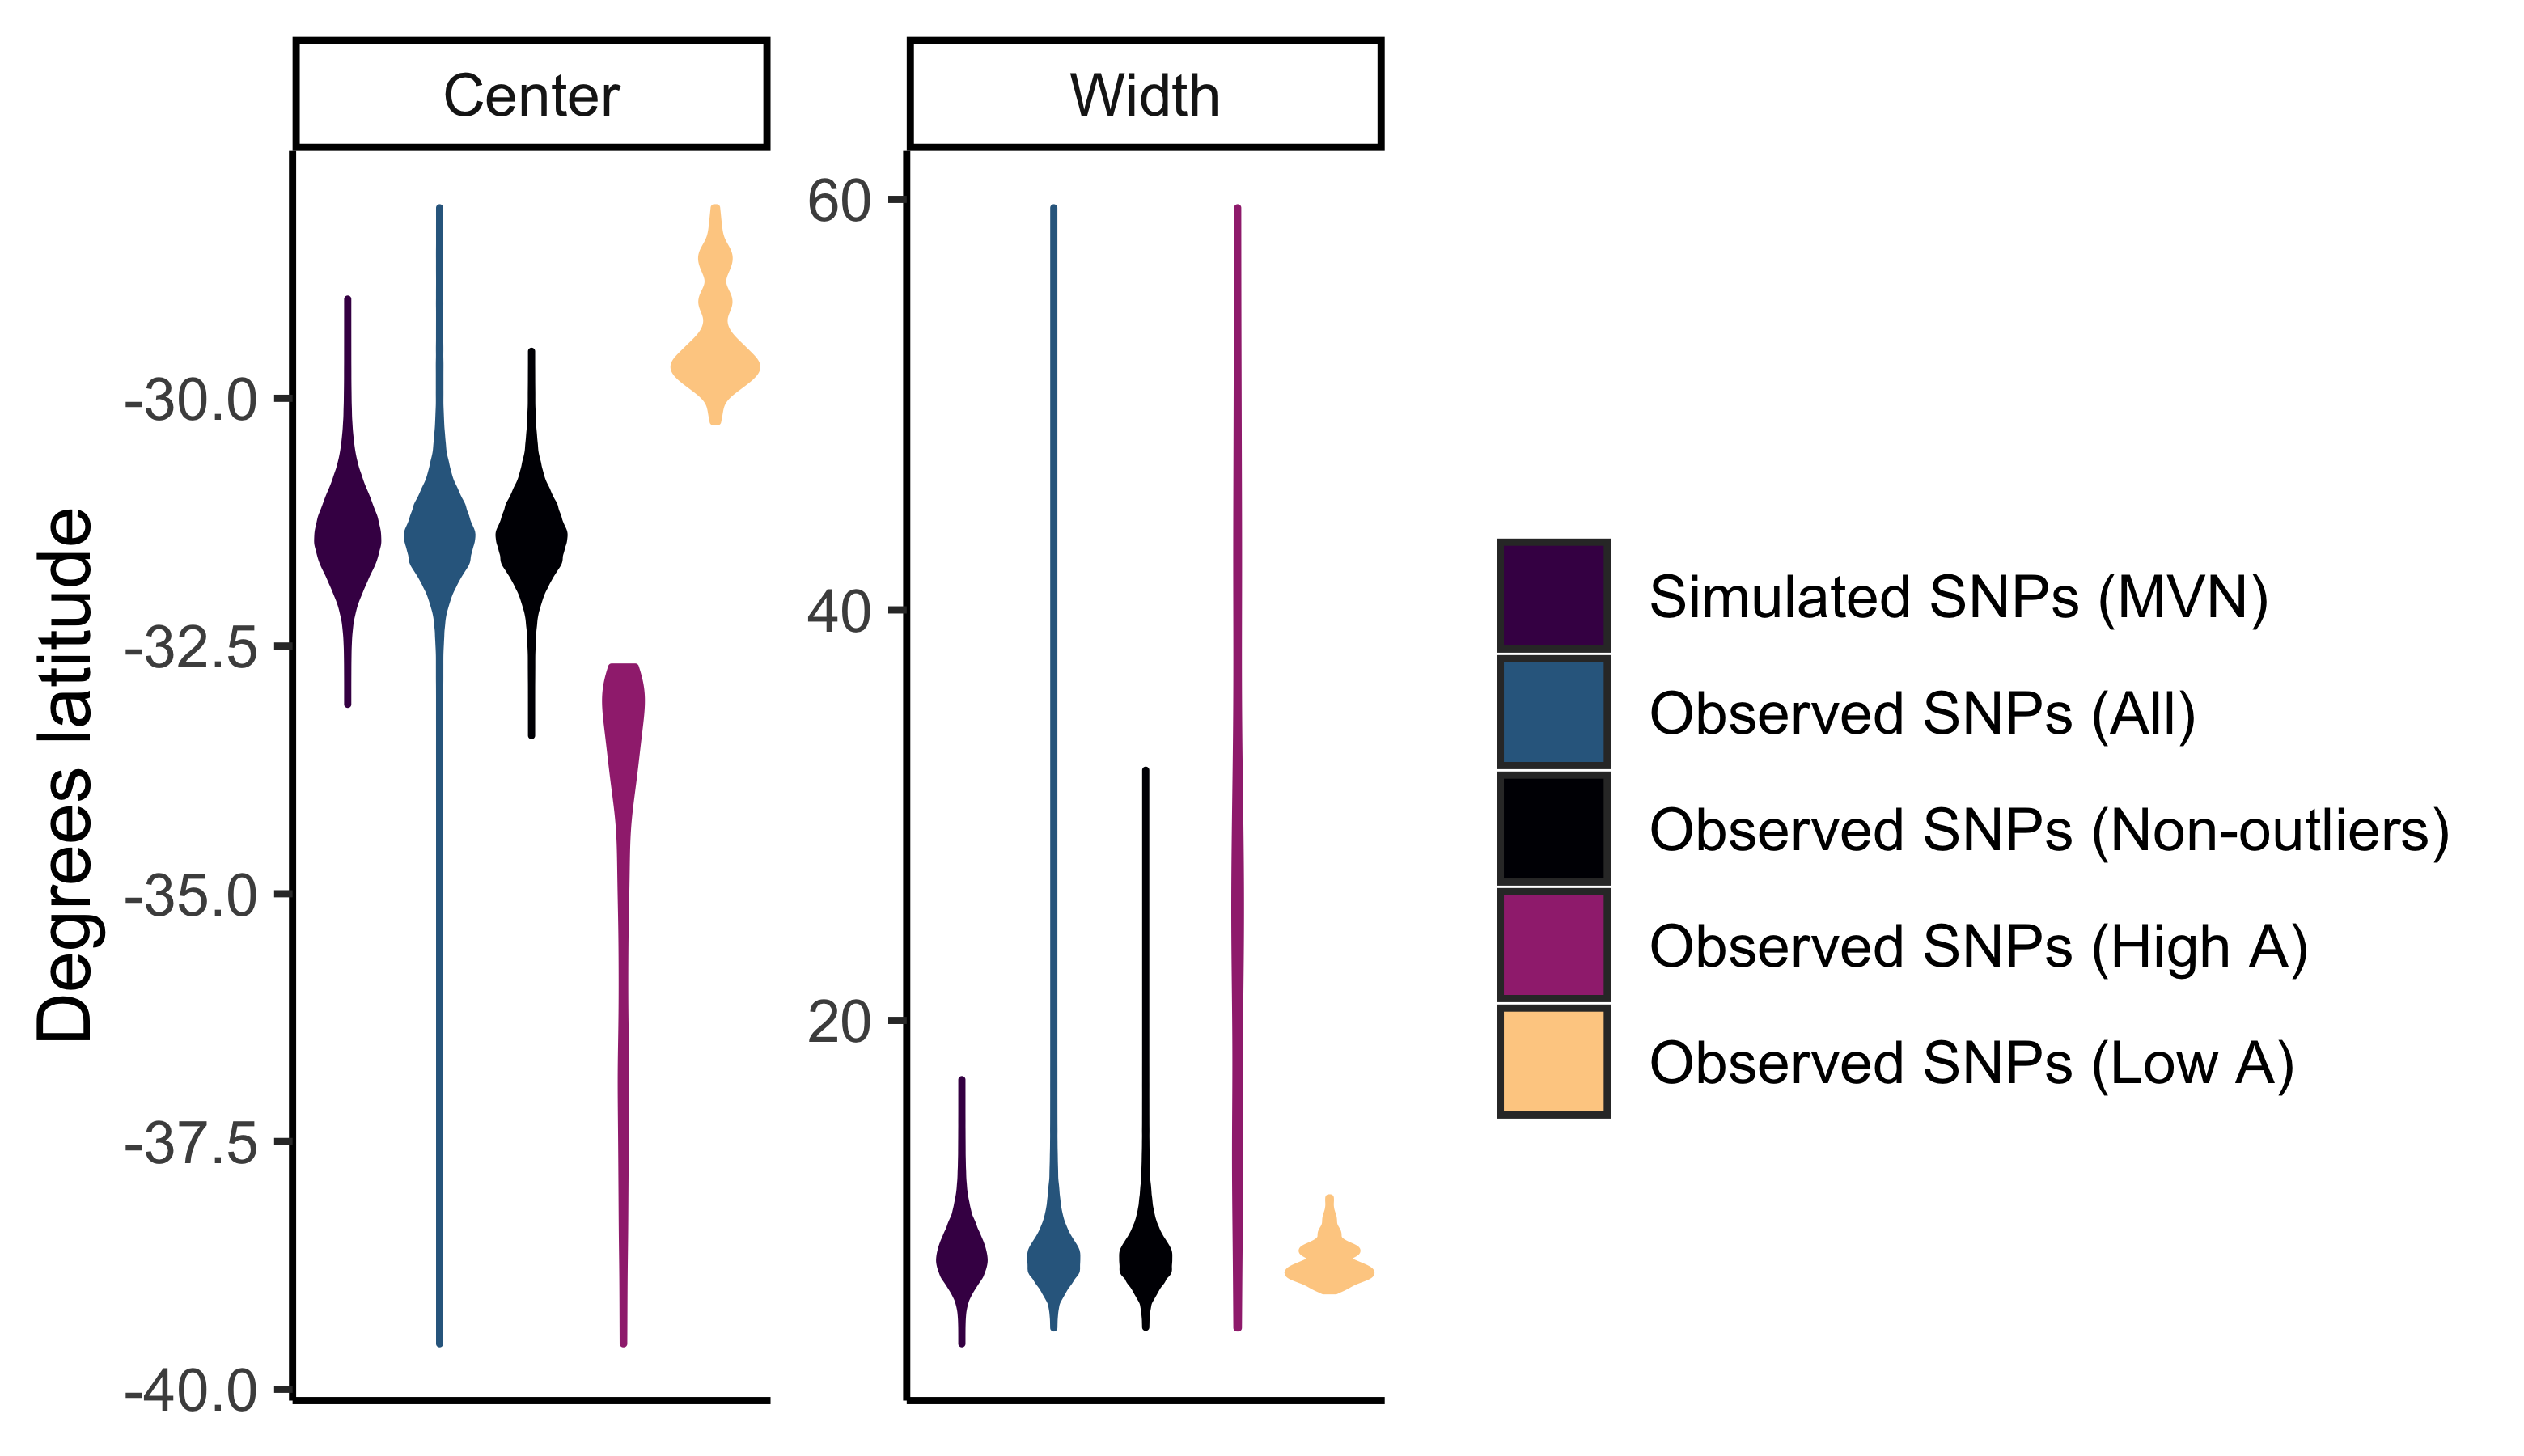
\includegraphics[width=\textwidth]{chapter1/figures/violin_ind_snp_clines.png}
\caption{ \textbf{Distribution of ancestry clines in South America across SNPs.} A logistic cline model was fit to observed and simulated population ancestry frequencies across latitude for S. America. Estimated cline parameters, center and width ($w = |\nicefrac{4}{b}|$), are presented as violin plots. Units for both cline center and width are degrees latitude. We additionally partition observed SNPs by outlier and non-outlier status, set by 10\% FDR for high or low \A\ ancestry in South America. Individual SNP clines were only fit in South America, where we observed the full cline.}
\label{violin_ind_clines}
\end{figure}



\begin{figure}[ht]
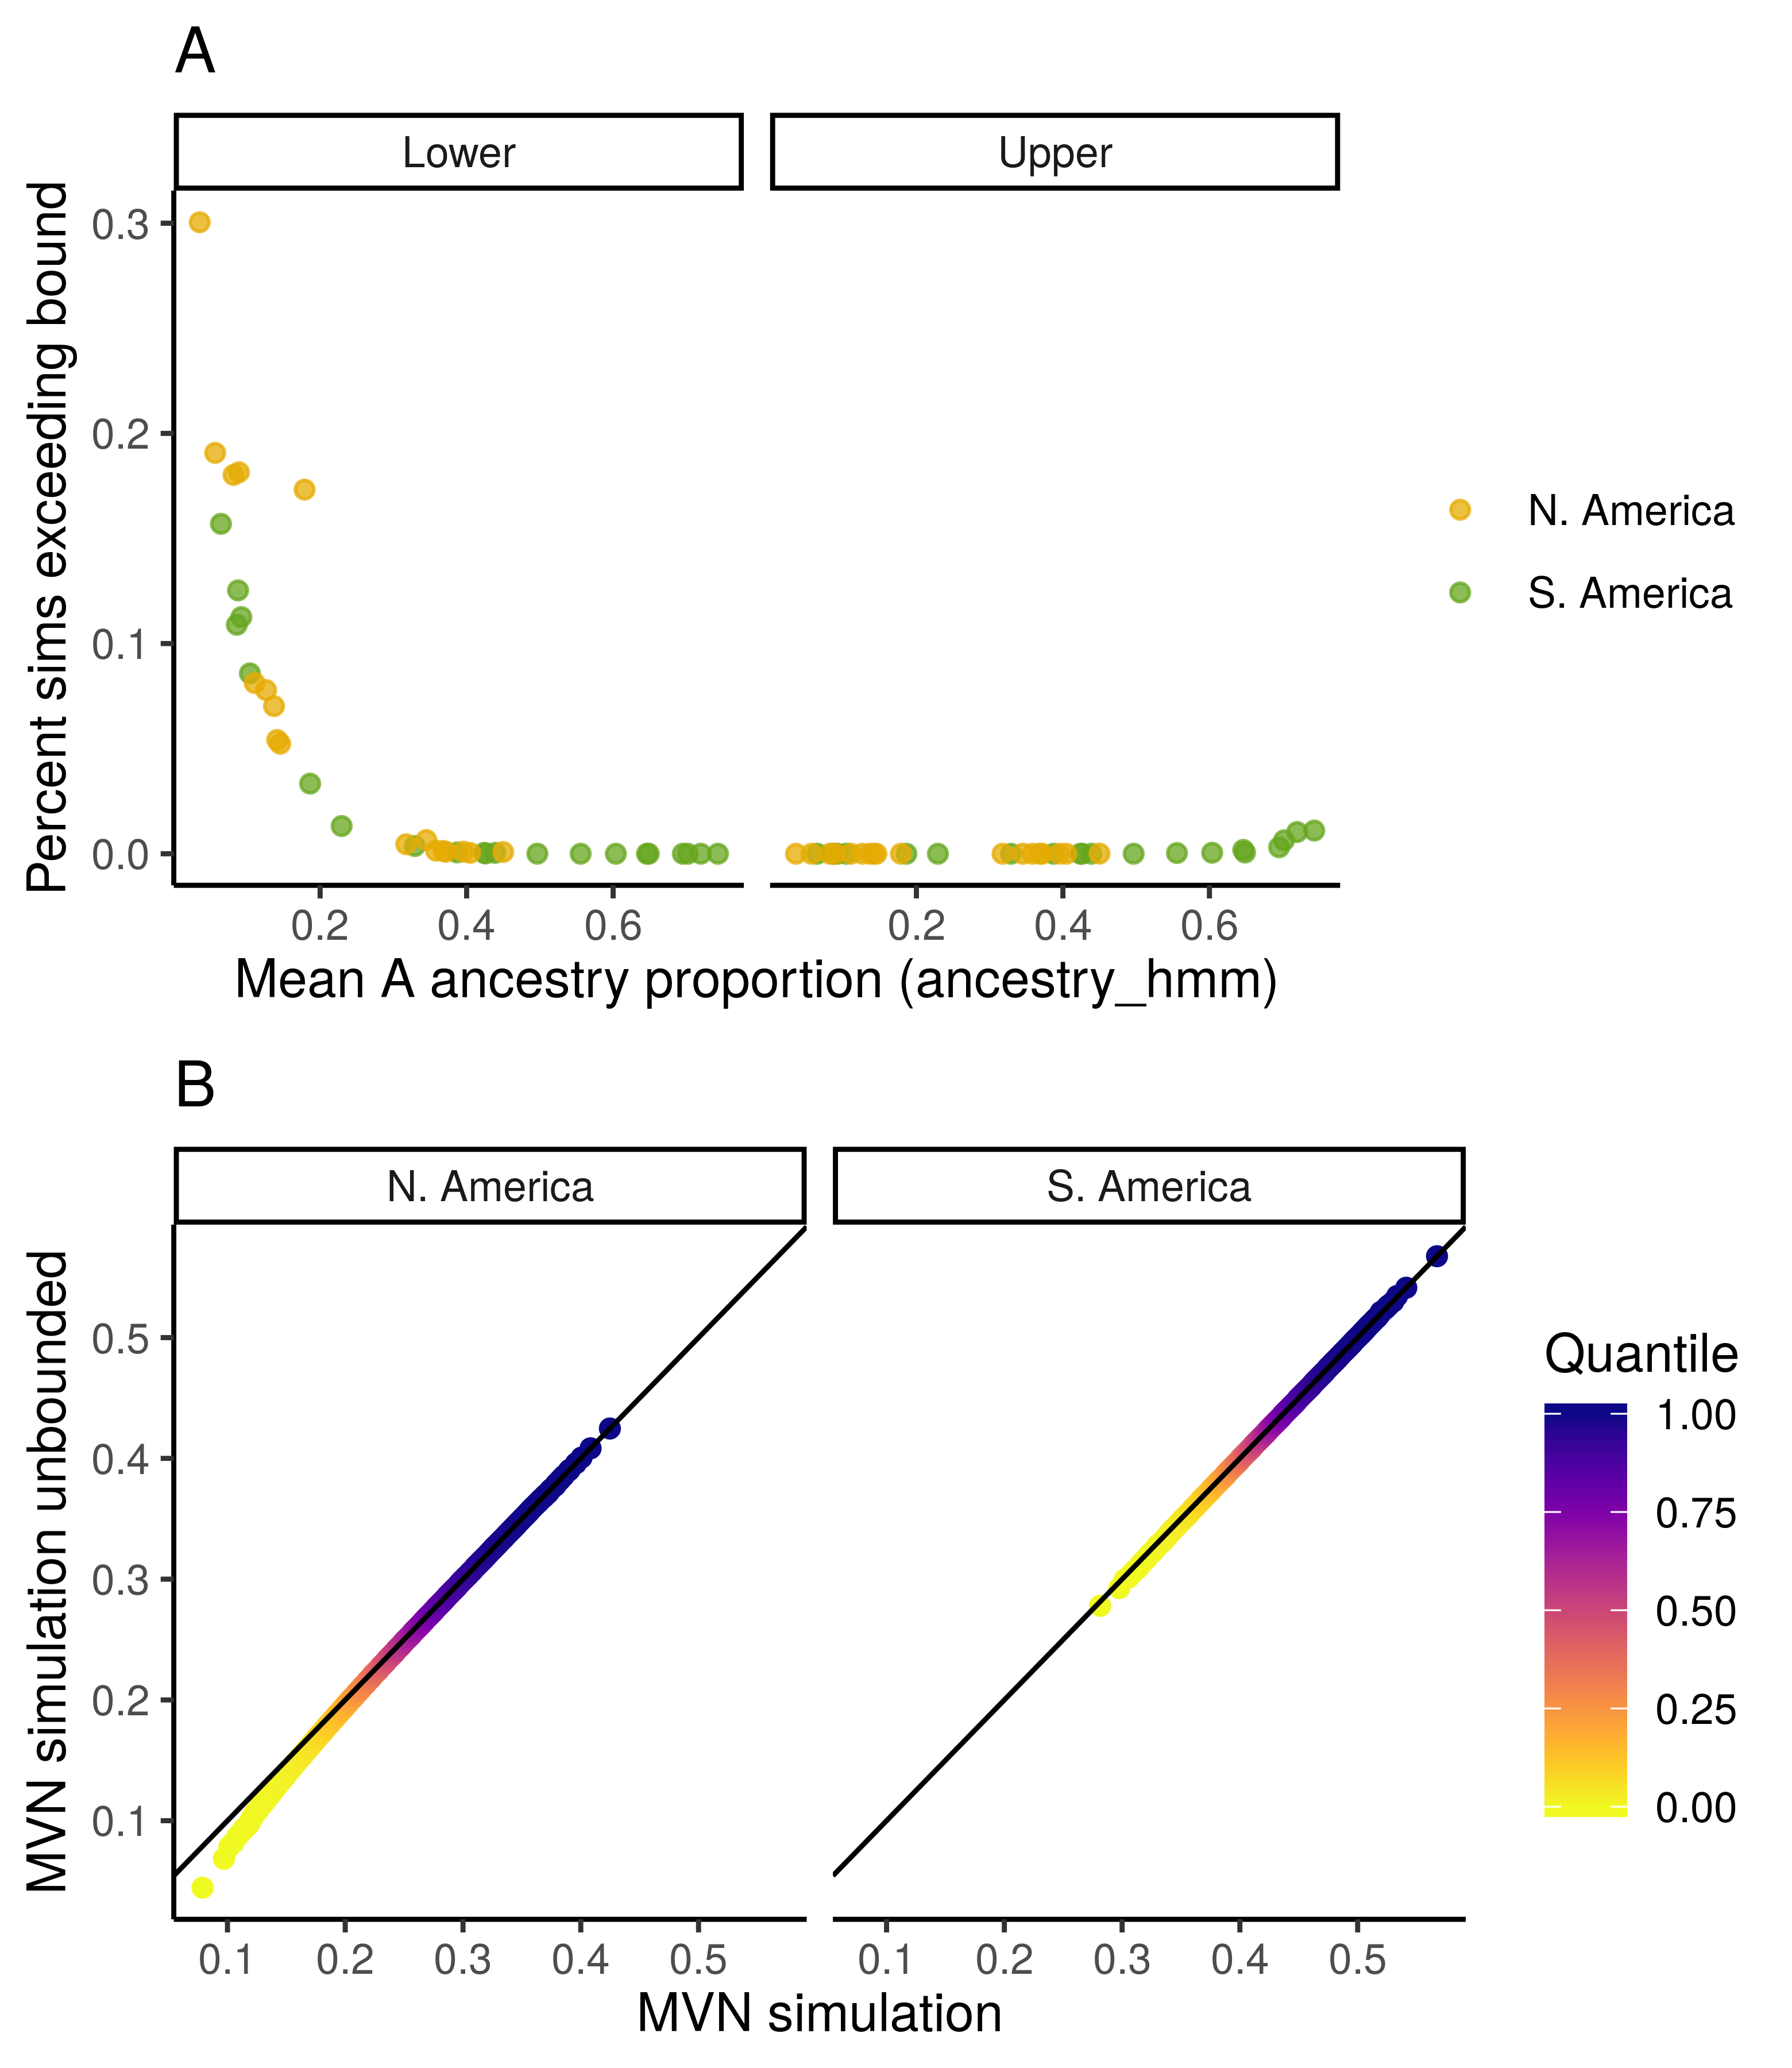
\includegraphics[width=.85\textwidth]{chapter1/figures/effect_truncation_on_MVN.png}
\caption{ \textbf{Effect of truncating MVN simulated ancestry frequencies.} (A) Percent of simulated population A-ancestry frequencies exceeding lower (left) and upper (right) bounds, and thus truncated to [0,1] range. Each population is a point and the populations most affected by truncation are low-A ancestry populations with mean A-ancestry proportions close to the bound at 0. (B) QQ-plot comparing the quantiles for mean A ancestry before and after truncation in N. America (left) and S. America (right). The distribution of mean \A\ ancestry is mostly unaffected by restricting simulated population A ancestry frequencies to the [0,1] range, but truncation does reduce model predictions of very low A-ancestry frequencies in N. America, where mean A ancestry is already low.}
\label{effect_truncation_mvn}
\end{figure}

\begin{figure}[ht]
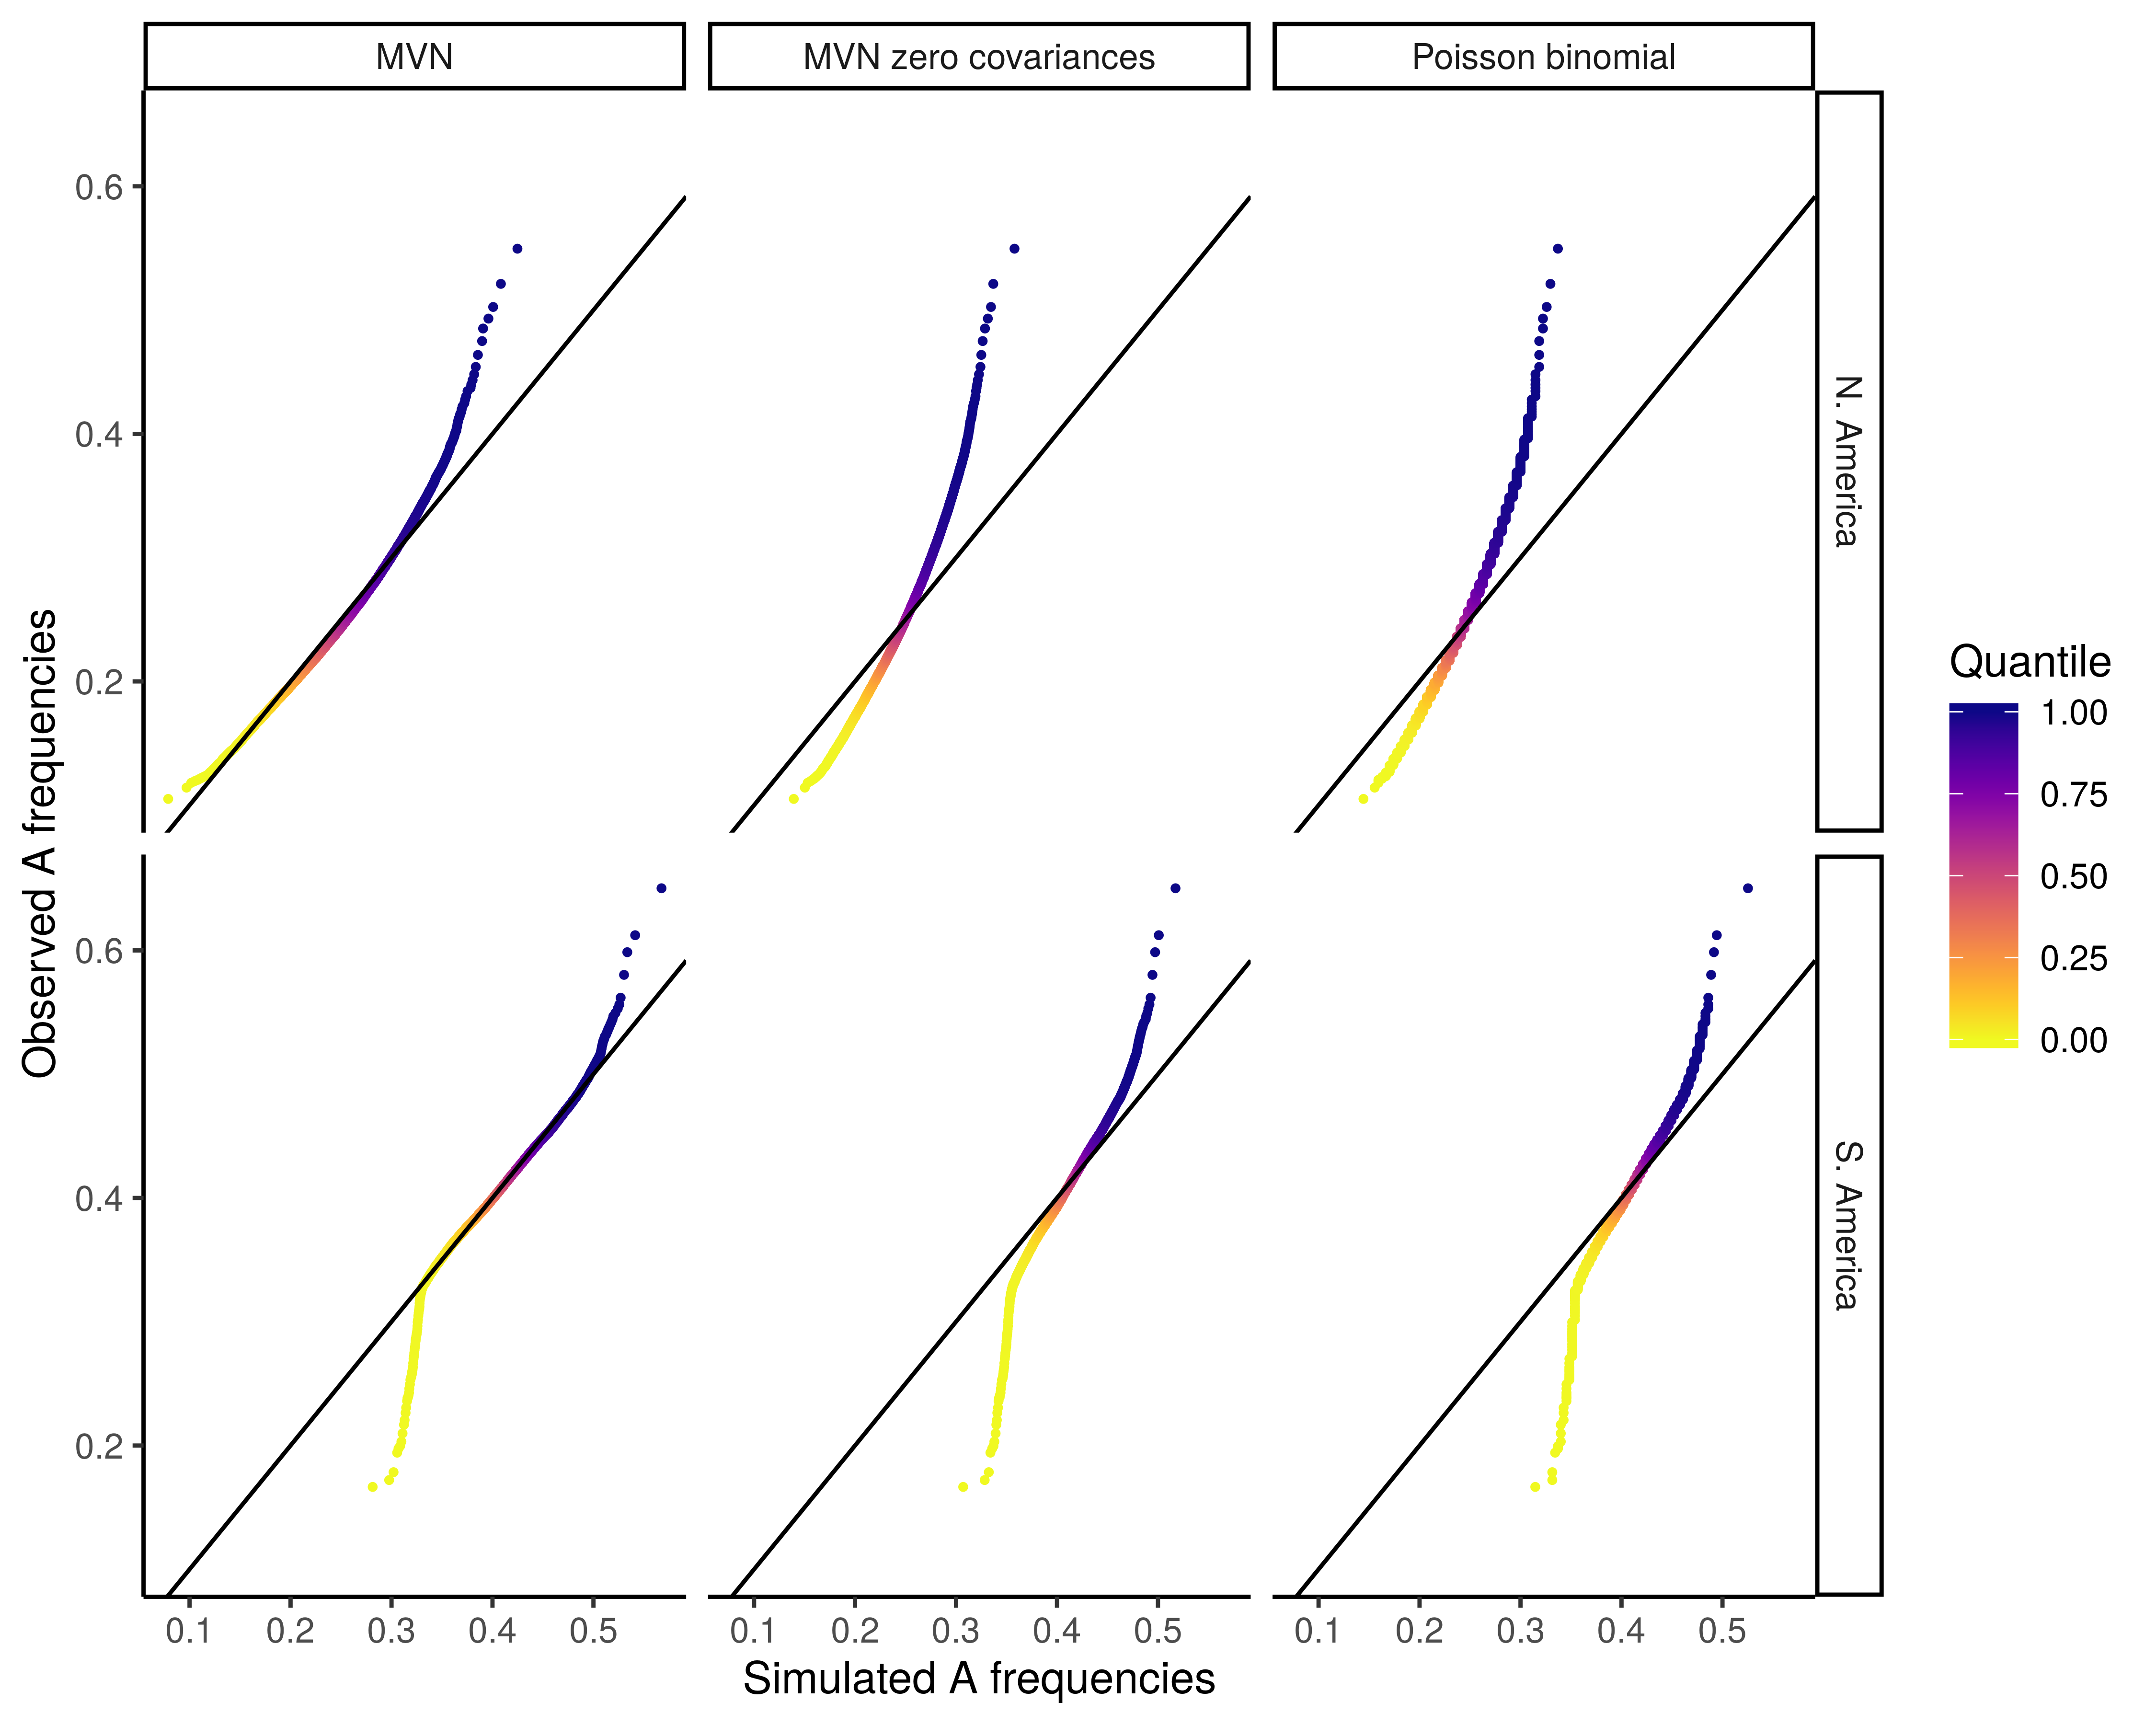
\includegraphics[width=\textwidth]{chapter1/figures/qq_vs_data_sim_comparison.png}
\caption{ \textbf{Simulated vs. observed \A\ ancestry quantiles}. QQ-plots comparing observed quantiles for mean \A\ ancestry in North America (top) and South America (bottom) to the quantiles generated by three simulated distributions (left-to-right): MVN, MVN with zero covariances, and Poisson binomial model. Only the MVN model, allowing for covariances between populations, matches the bulk of the observed distribution.}
\label{qq_data_sims}
\end{figure}

\begin{figure}[ht]
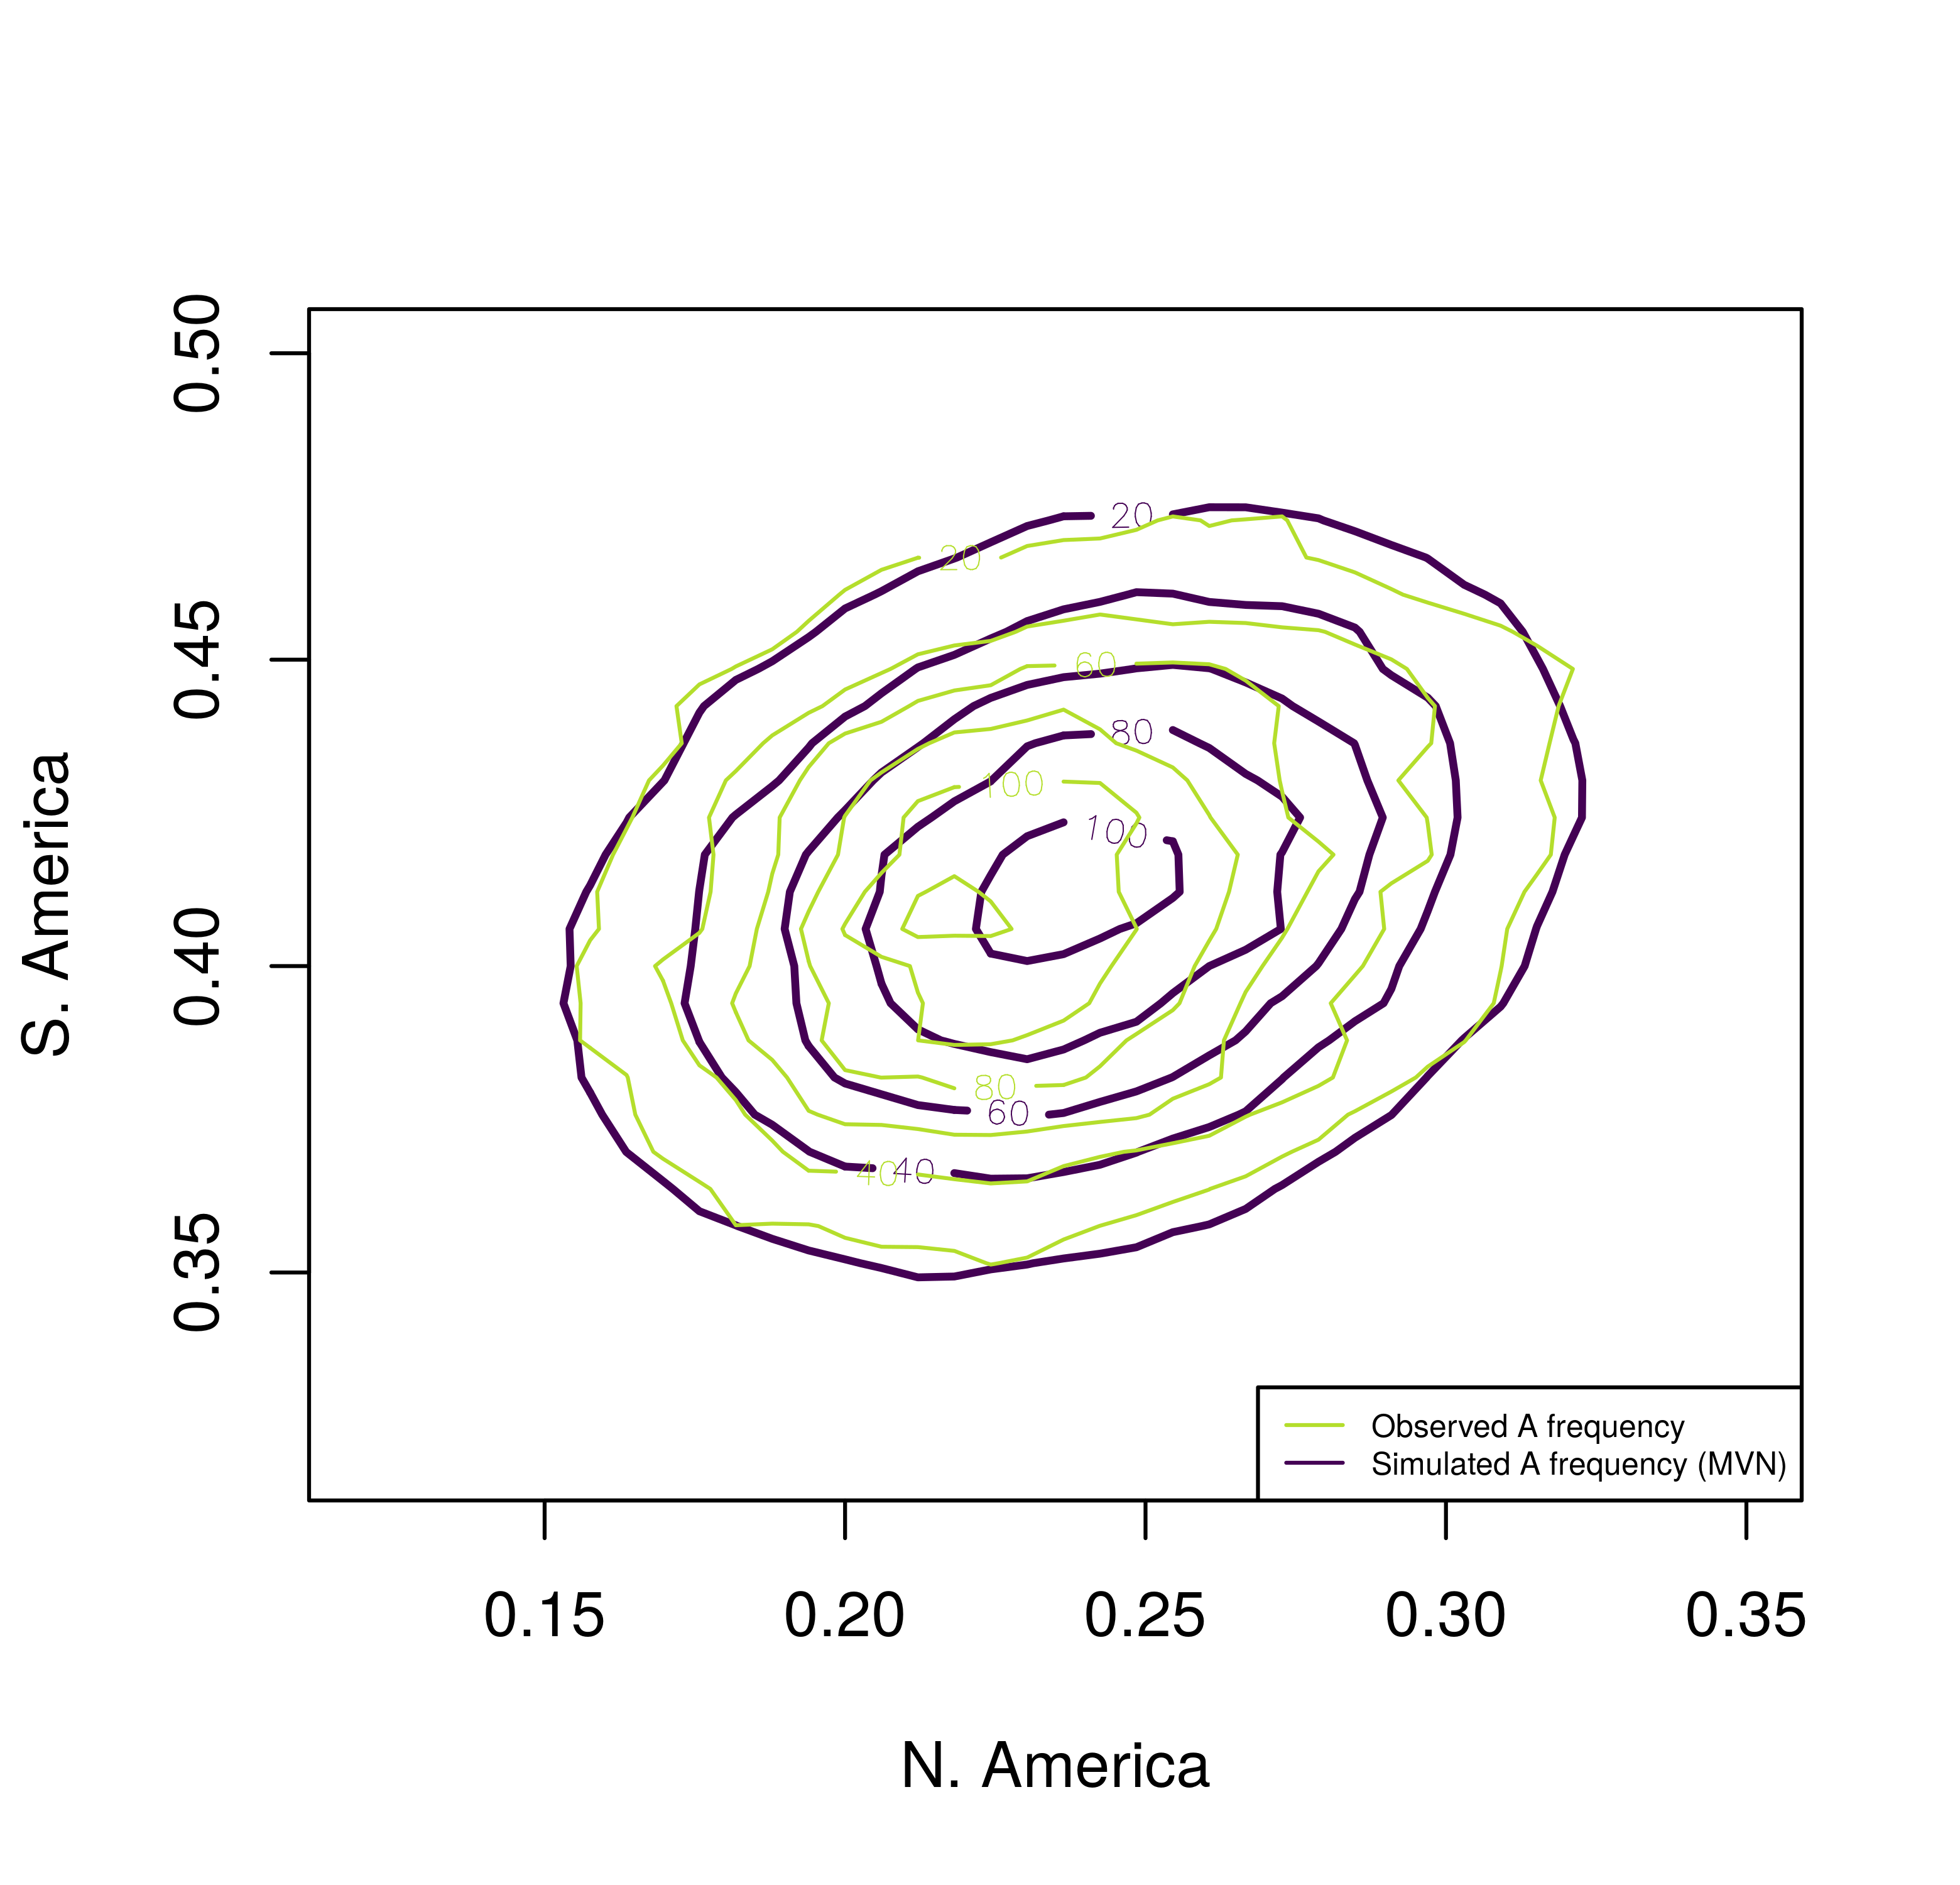
\includegraphics[width=\textwidth]{chapter1/figures/comparison_2d_density_data_mvn.png}
\caption{ \textbf{Overlay of 2D density plot for observed A ancestry frequencies in North and South America compared to simulated A ancestry frequencies under a multivariate-normal model.}}
\label{density_data_mvn}
\end{figure}

\begin{figure}[ht]
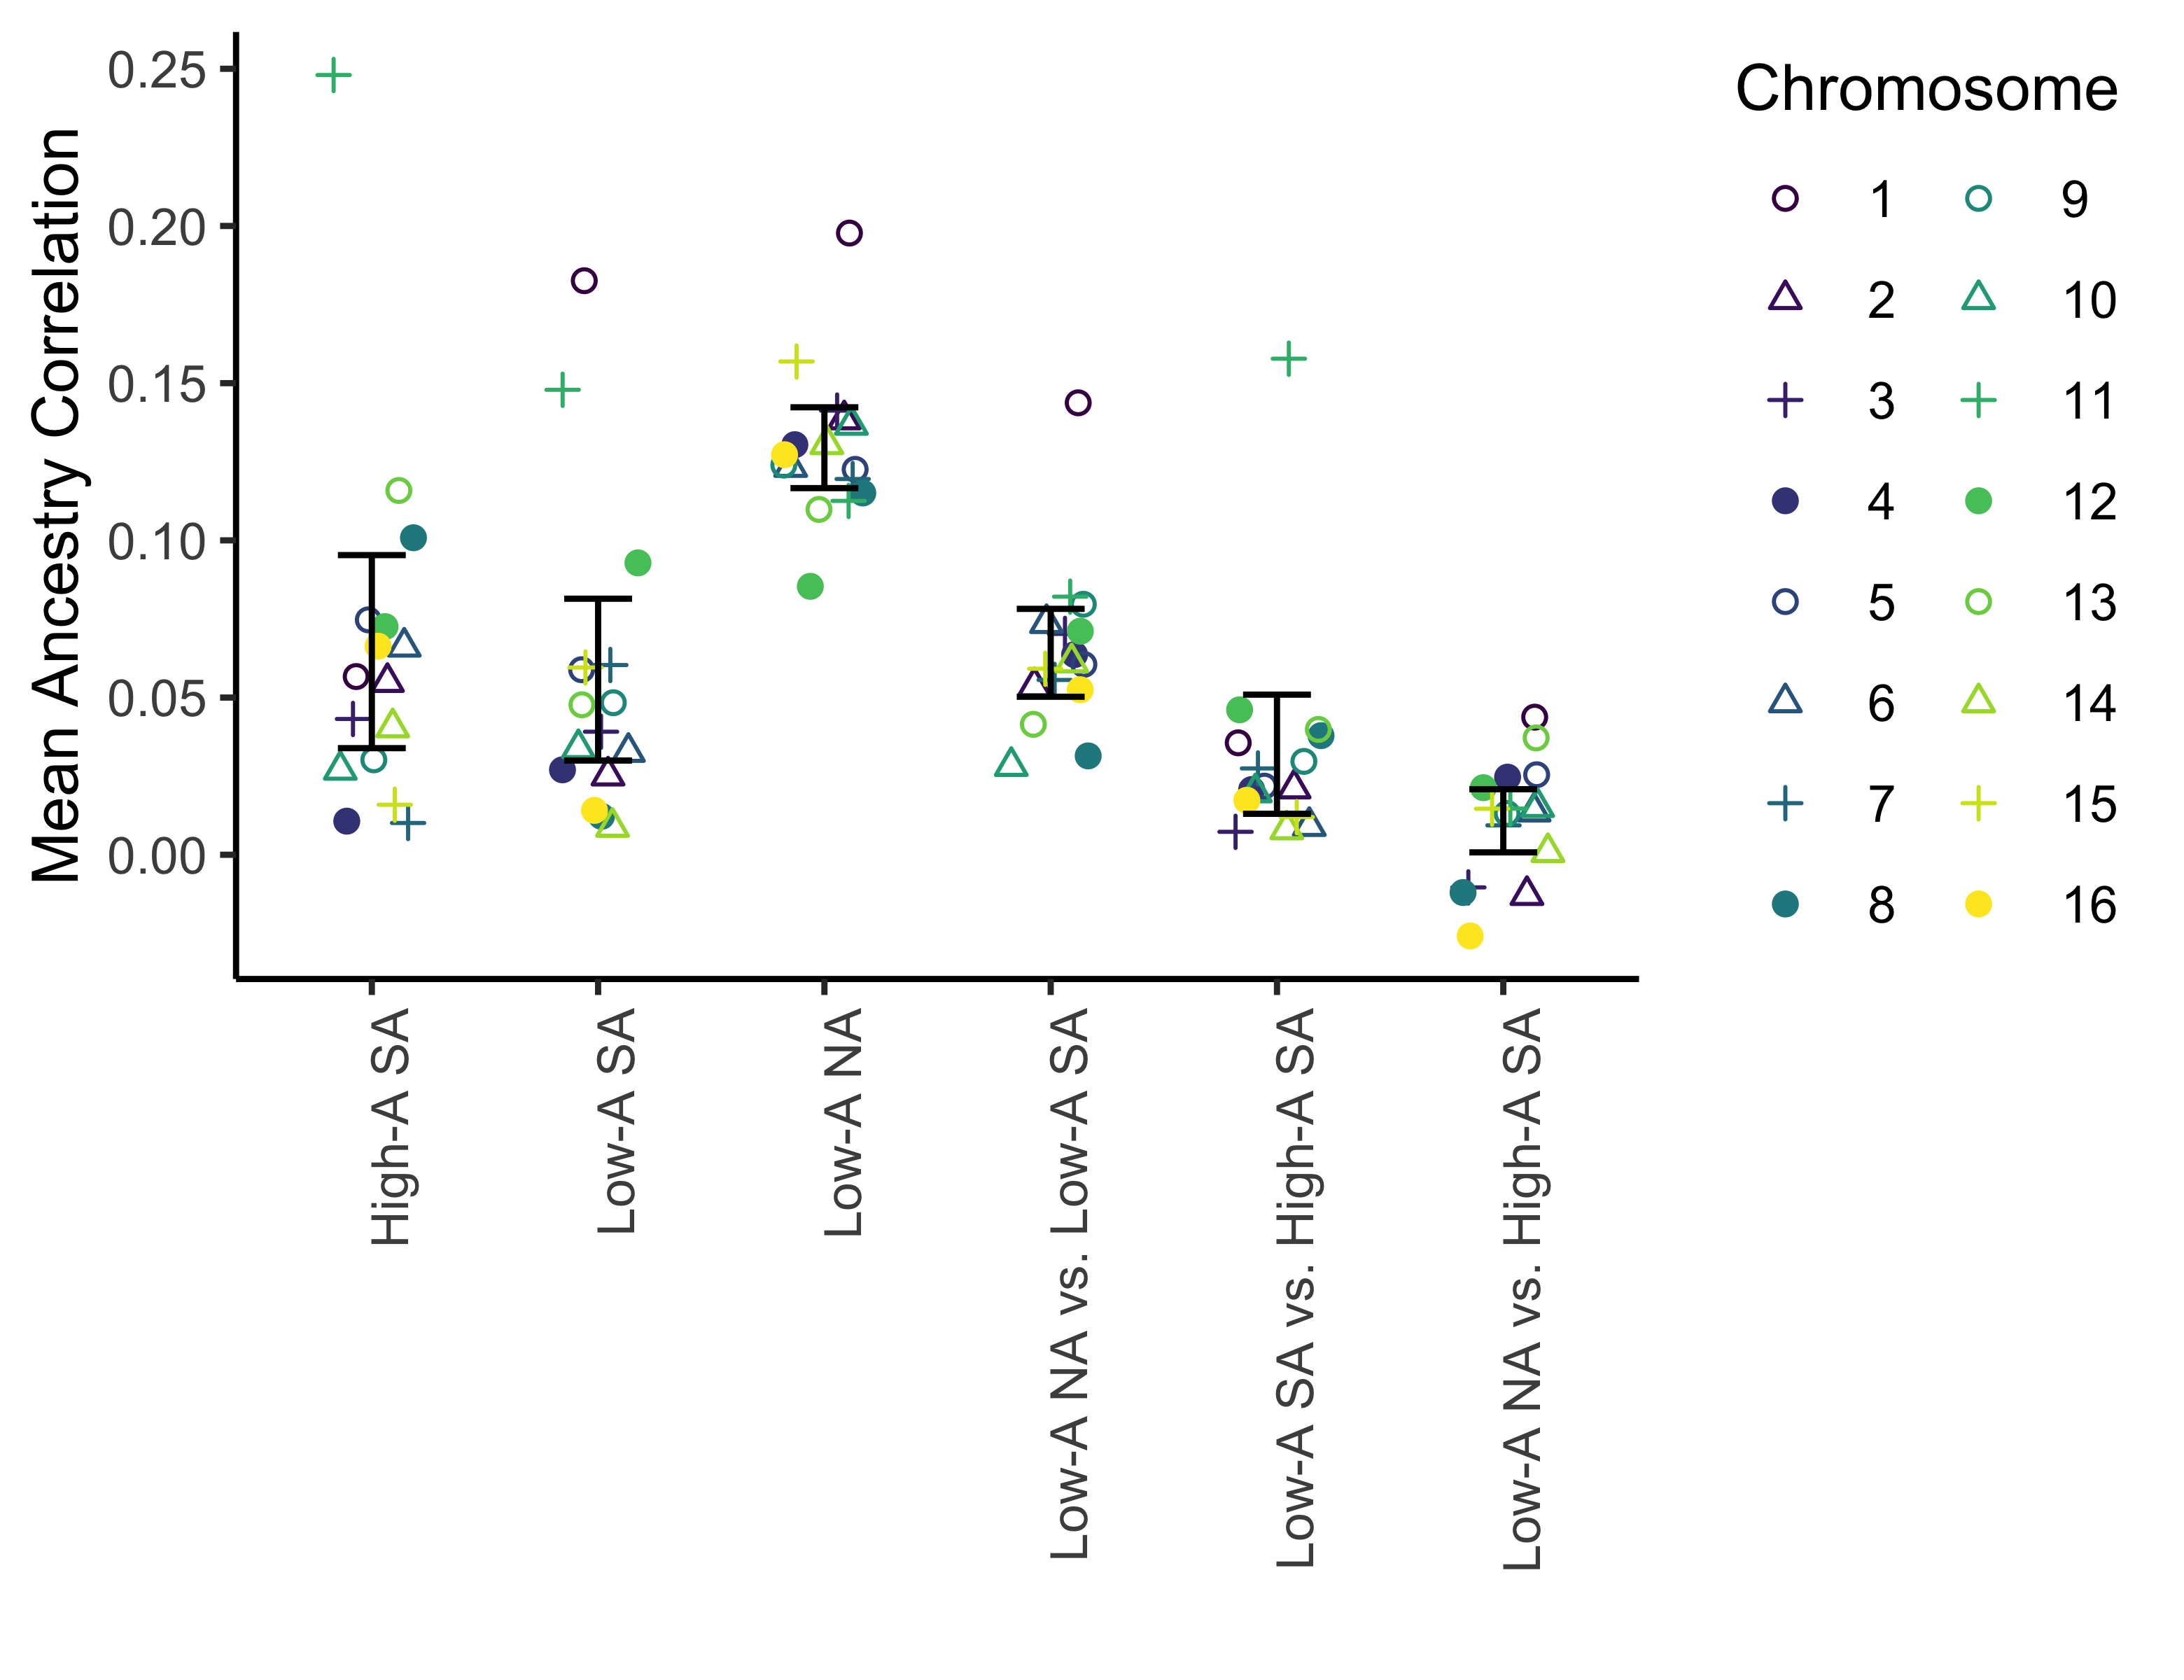
\includegraphics[width=\textwidth]{chapter1/figures/mean_k_corr_by_groups_and_chr.png}
\caption{ \textbf{Mean ancestry correlation by chromosome across populations.} Mean ancestry covariances (K matrices) were calculated separately for \edit{each} chromosome, using the genome-wide mean ancestry as $\alpha$, then correlations were summarised by taking the mean for each type of population comparison, within and between continents and \ec{low vs. high A} regions. Error bars show the normal-approximated 95\% confidence intervals around these means. We divided populations in South America into \edit{low A and high A} groups \edit{relative to the cline center}. \ec{Low A populations are found at higher latitudes and correspondingly cooler climates}. All North American samples come from the \ec{low-A} side of the cline. On average across chromosomes, \ec{low-A} South American populations share higher ancestry correlations with \ec{low-A} North American populations than with geographically closer \ec{high-A} South American populations \ec{(0.032: CI$_{95}[0.011, .053]$, P = .005, paired 2-sided t-test)}. Two chromosomes harbor large outlier regions consistent with their elevated correlations shown here: Chromosome 1 has a large cluster of loci with high A ancestry in North and South America while chromosome 11 has a wide region of low A ancestry exclusive to South America. The results do not change qualitatively if these two outlier chromosomes are both removed from the analysis \ec{(0.035: CI$_{95}[0.022, 0.047]$, P = $4.8x10^{-5}$, paired 2-sided t-test).}}
\label{fig_mean_k_by_chr}
\end{figure}

\begin{figure}[ht]
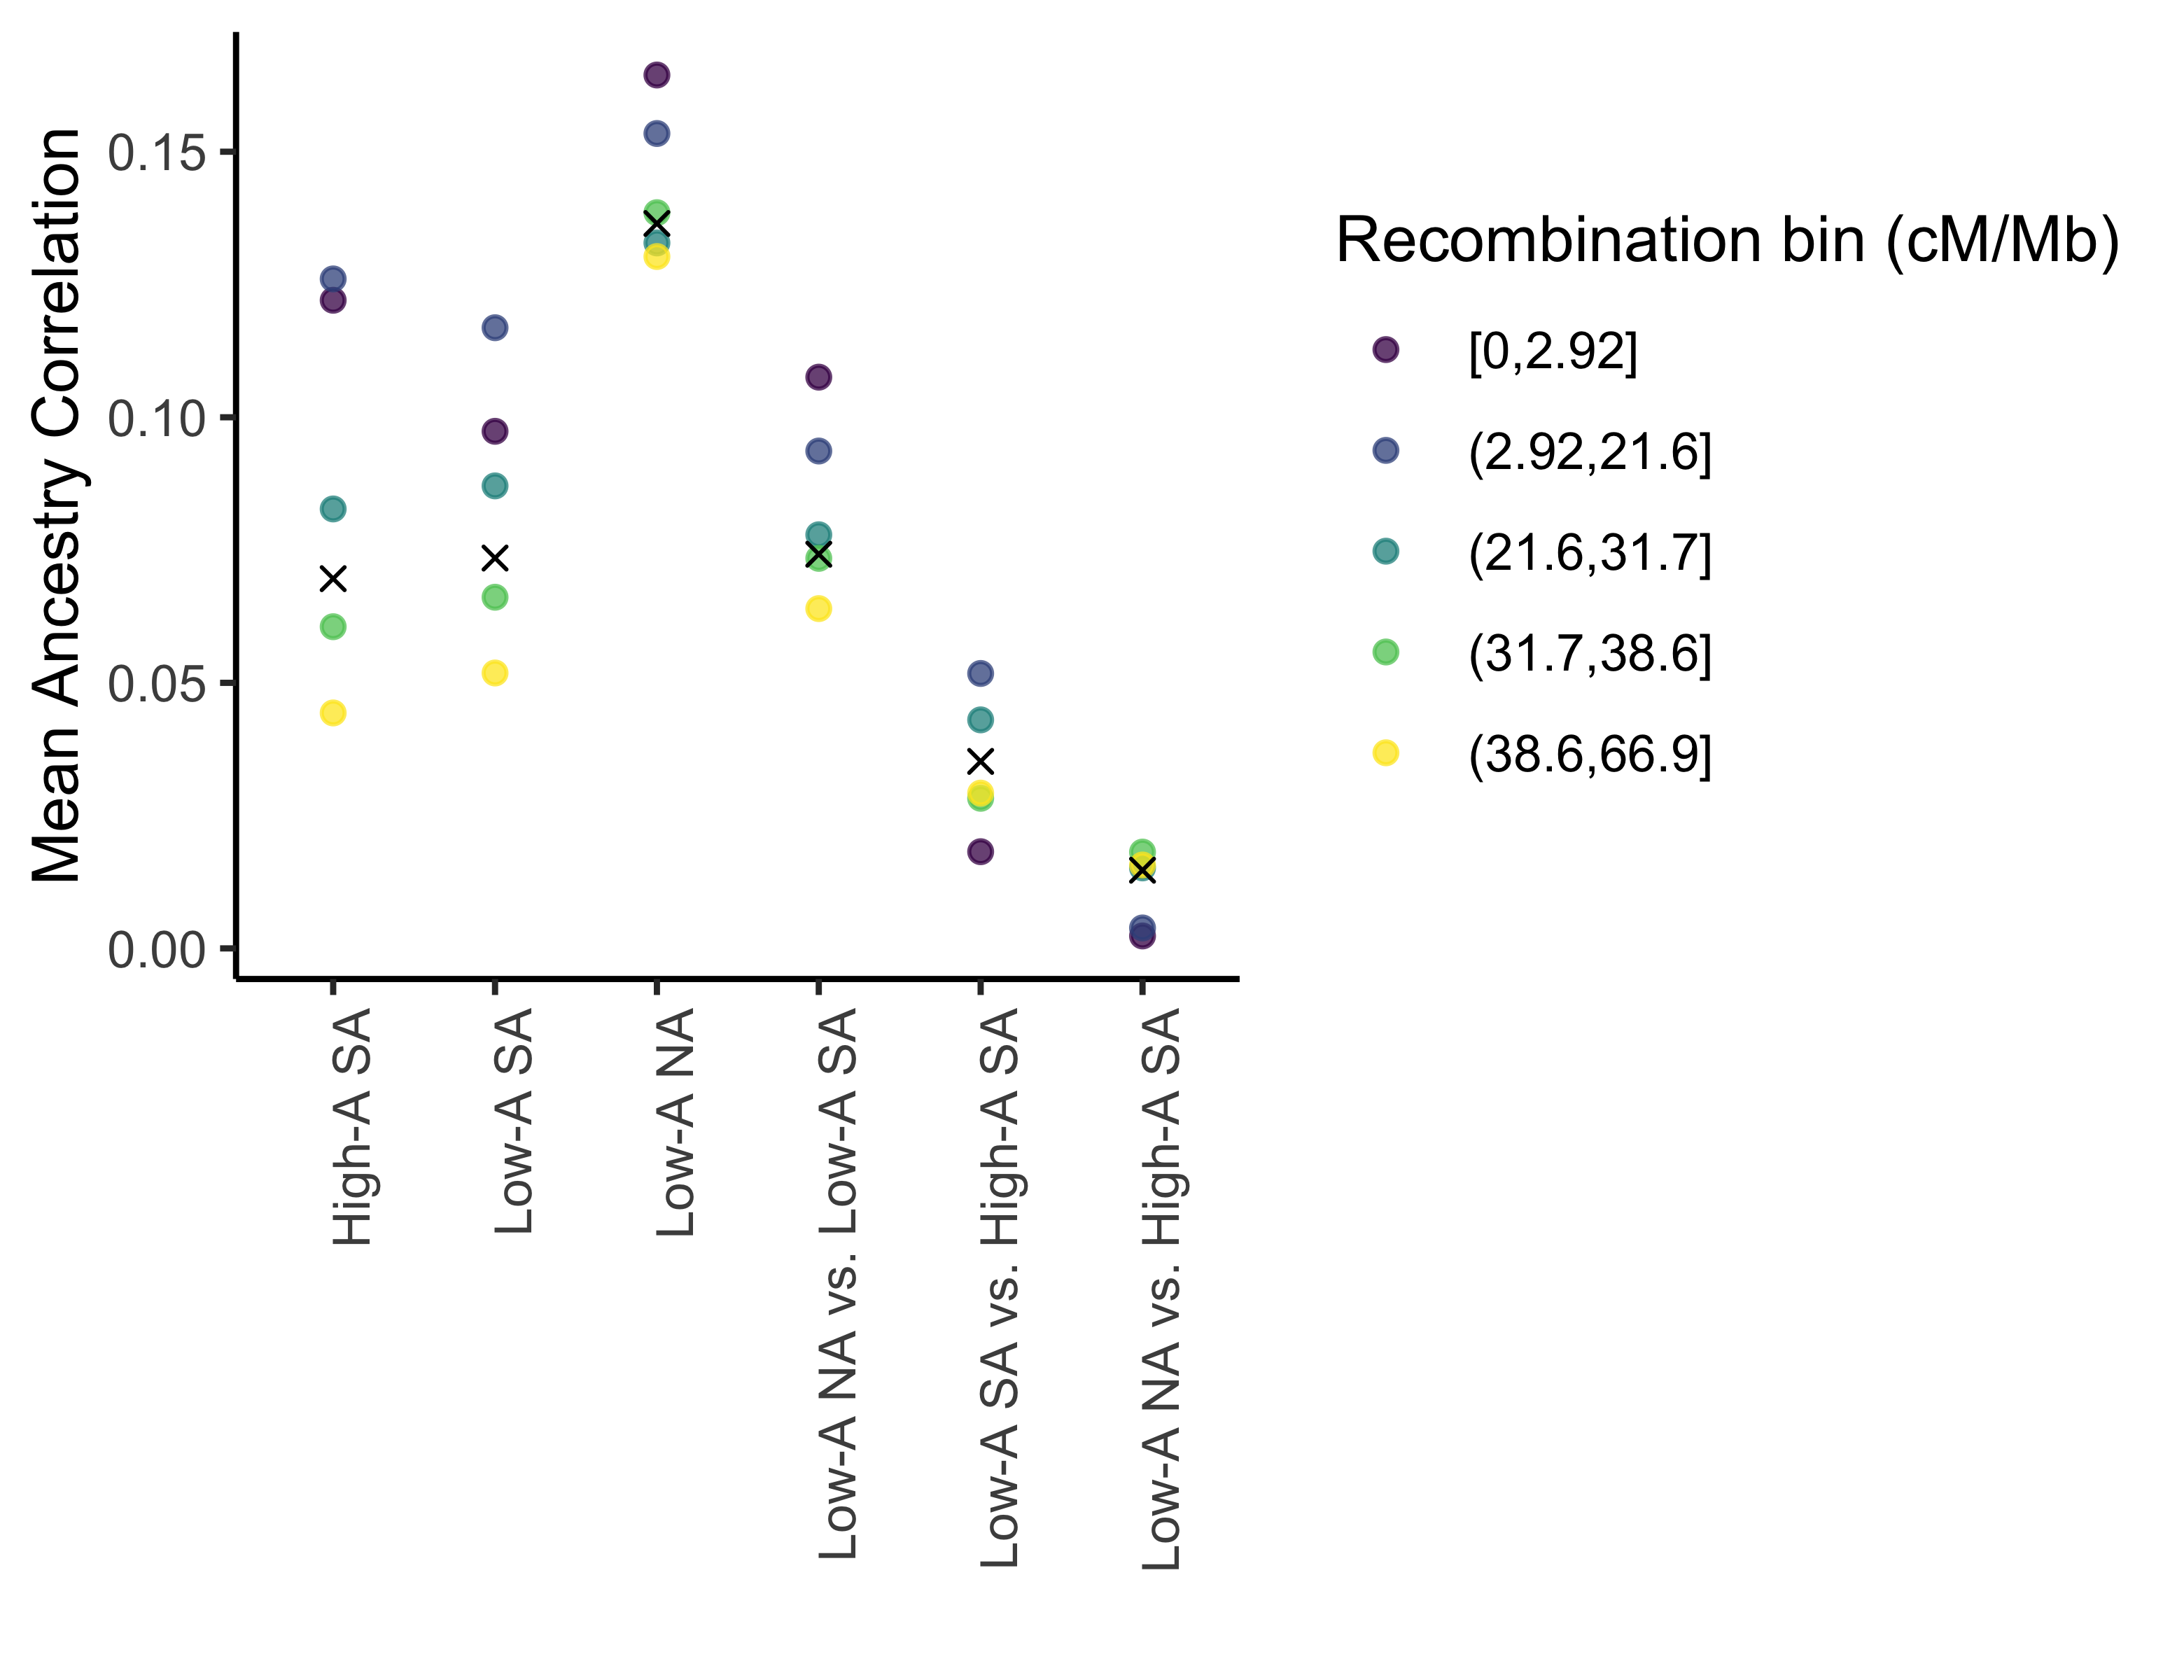
\includegraphics[width=\textwidth]{chapter1/figures/mean_k_corr_by_groups_and_r.png}
\caption{ \textbf{Mean correlation for population pairs by recombination rate.} Mean ancestry covariances (K matrices) were calculated separately for each of the 5 recombination rate quintiles, using the genome-wide mean ancestry as $\alpha$, then correlations were summarised by taking the mean for each type of population comparison, within and between continents and \ec{low vs. high A} regions. \ec{About half of the South American populations, and all of the sampled North American populations come from the \ec{low-A} side of the hybrid zone (relative to the estimated cline center).} The genomewide mean is additionally shown as an X. On average across recombination bins, \ec{low-A} South American populations share higher ancestry correlations with \ec{low-A} North American populations than with geographically closer \ec{high-A} South American populations \ec{(0.049: CI$_{95}[0.021, .078]$, P = .009, paired 2-sided t-test)}}
\label{fig_mean_k_by_r}
\end{figure}

\begin{figure}[ht]
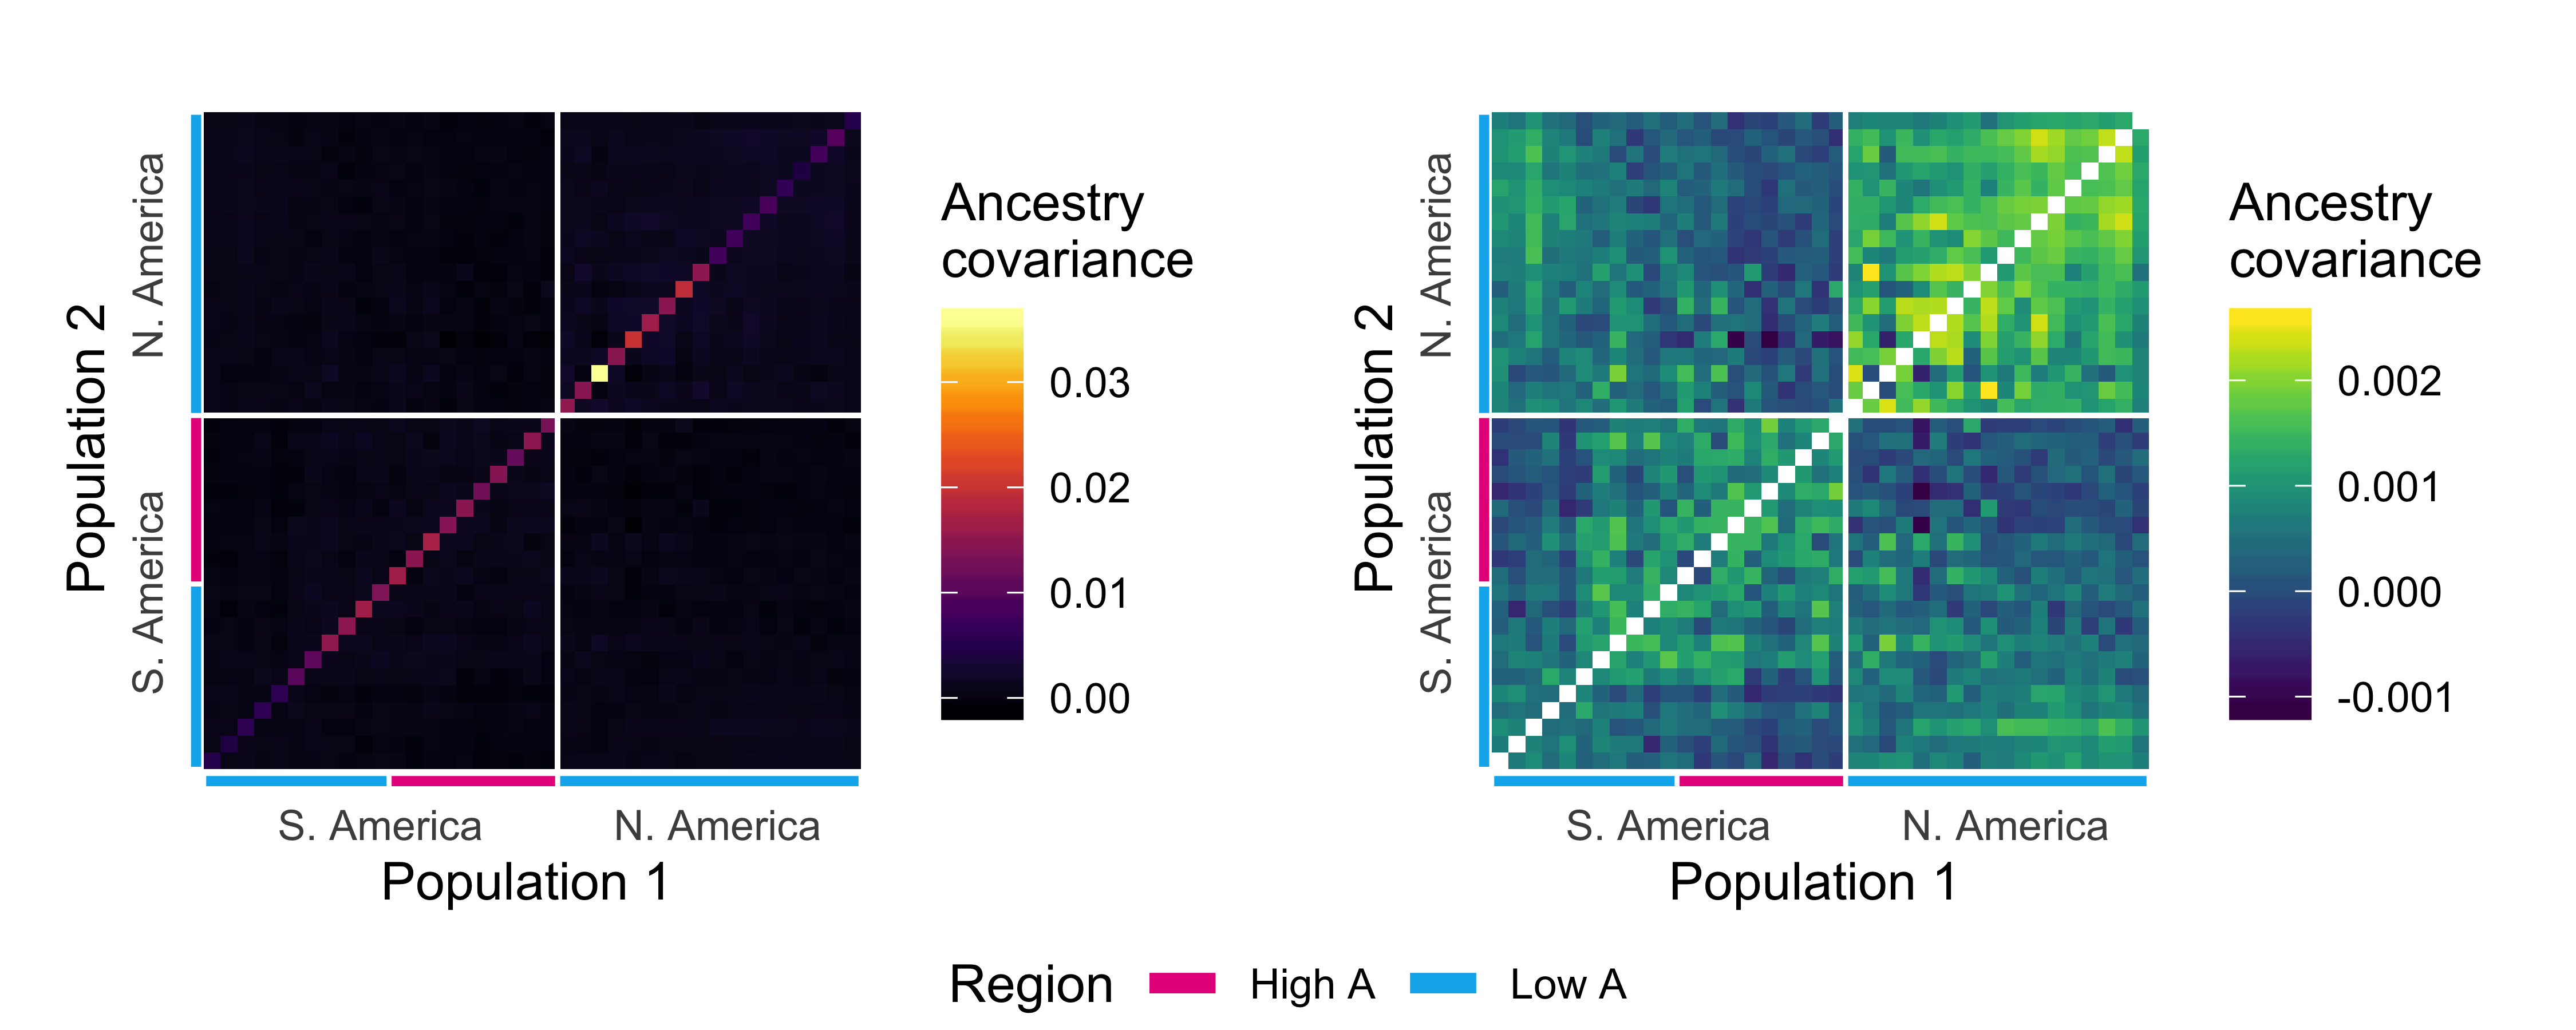
\includegraphics[width=\textwidth]{chapter1/figures/k_covariance_matrix_all_pops.png}
\caption{\ec{\textbf{Ancestry covariances across populations.} Ancestry covariance matrix (see methods). Populations are ordered by latitude, with high and low A sides of each hybrid zone defined relative to the estimated genomewide cline center. Within-population variances (left) are shown separately from between-population covariances (right) because of the drastically different scales. Populations near the cline center have higher ancestry variances (most clearly seen in the diagonal elements) because they have \A\ ancestry proportions closer to 50\%. Drift and finite sample sizes also contribute to the observed ancestry variances. The third lowest latitude population in the North American cline with exceptionally high ancestry variance is Avalon, sampled from Catalina Island off the coast of California. The observed excess covariance between the two distant ends of these clines is unexpected under a simple model of spread North and South out of Brazil.}}
\label{k_cov_matrix}
\end{figure}


\begin{figure}[ht]
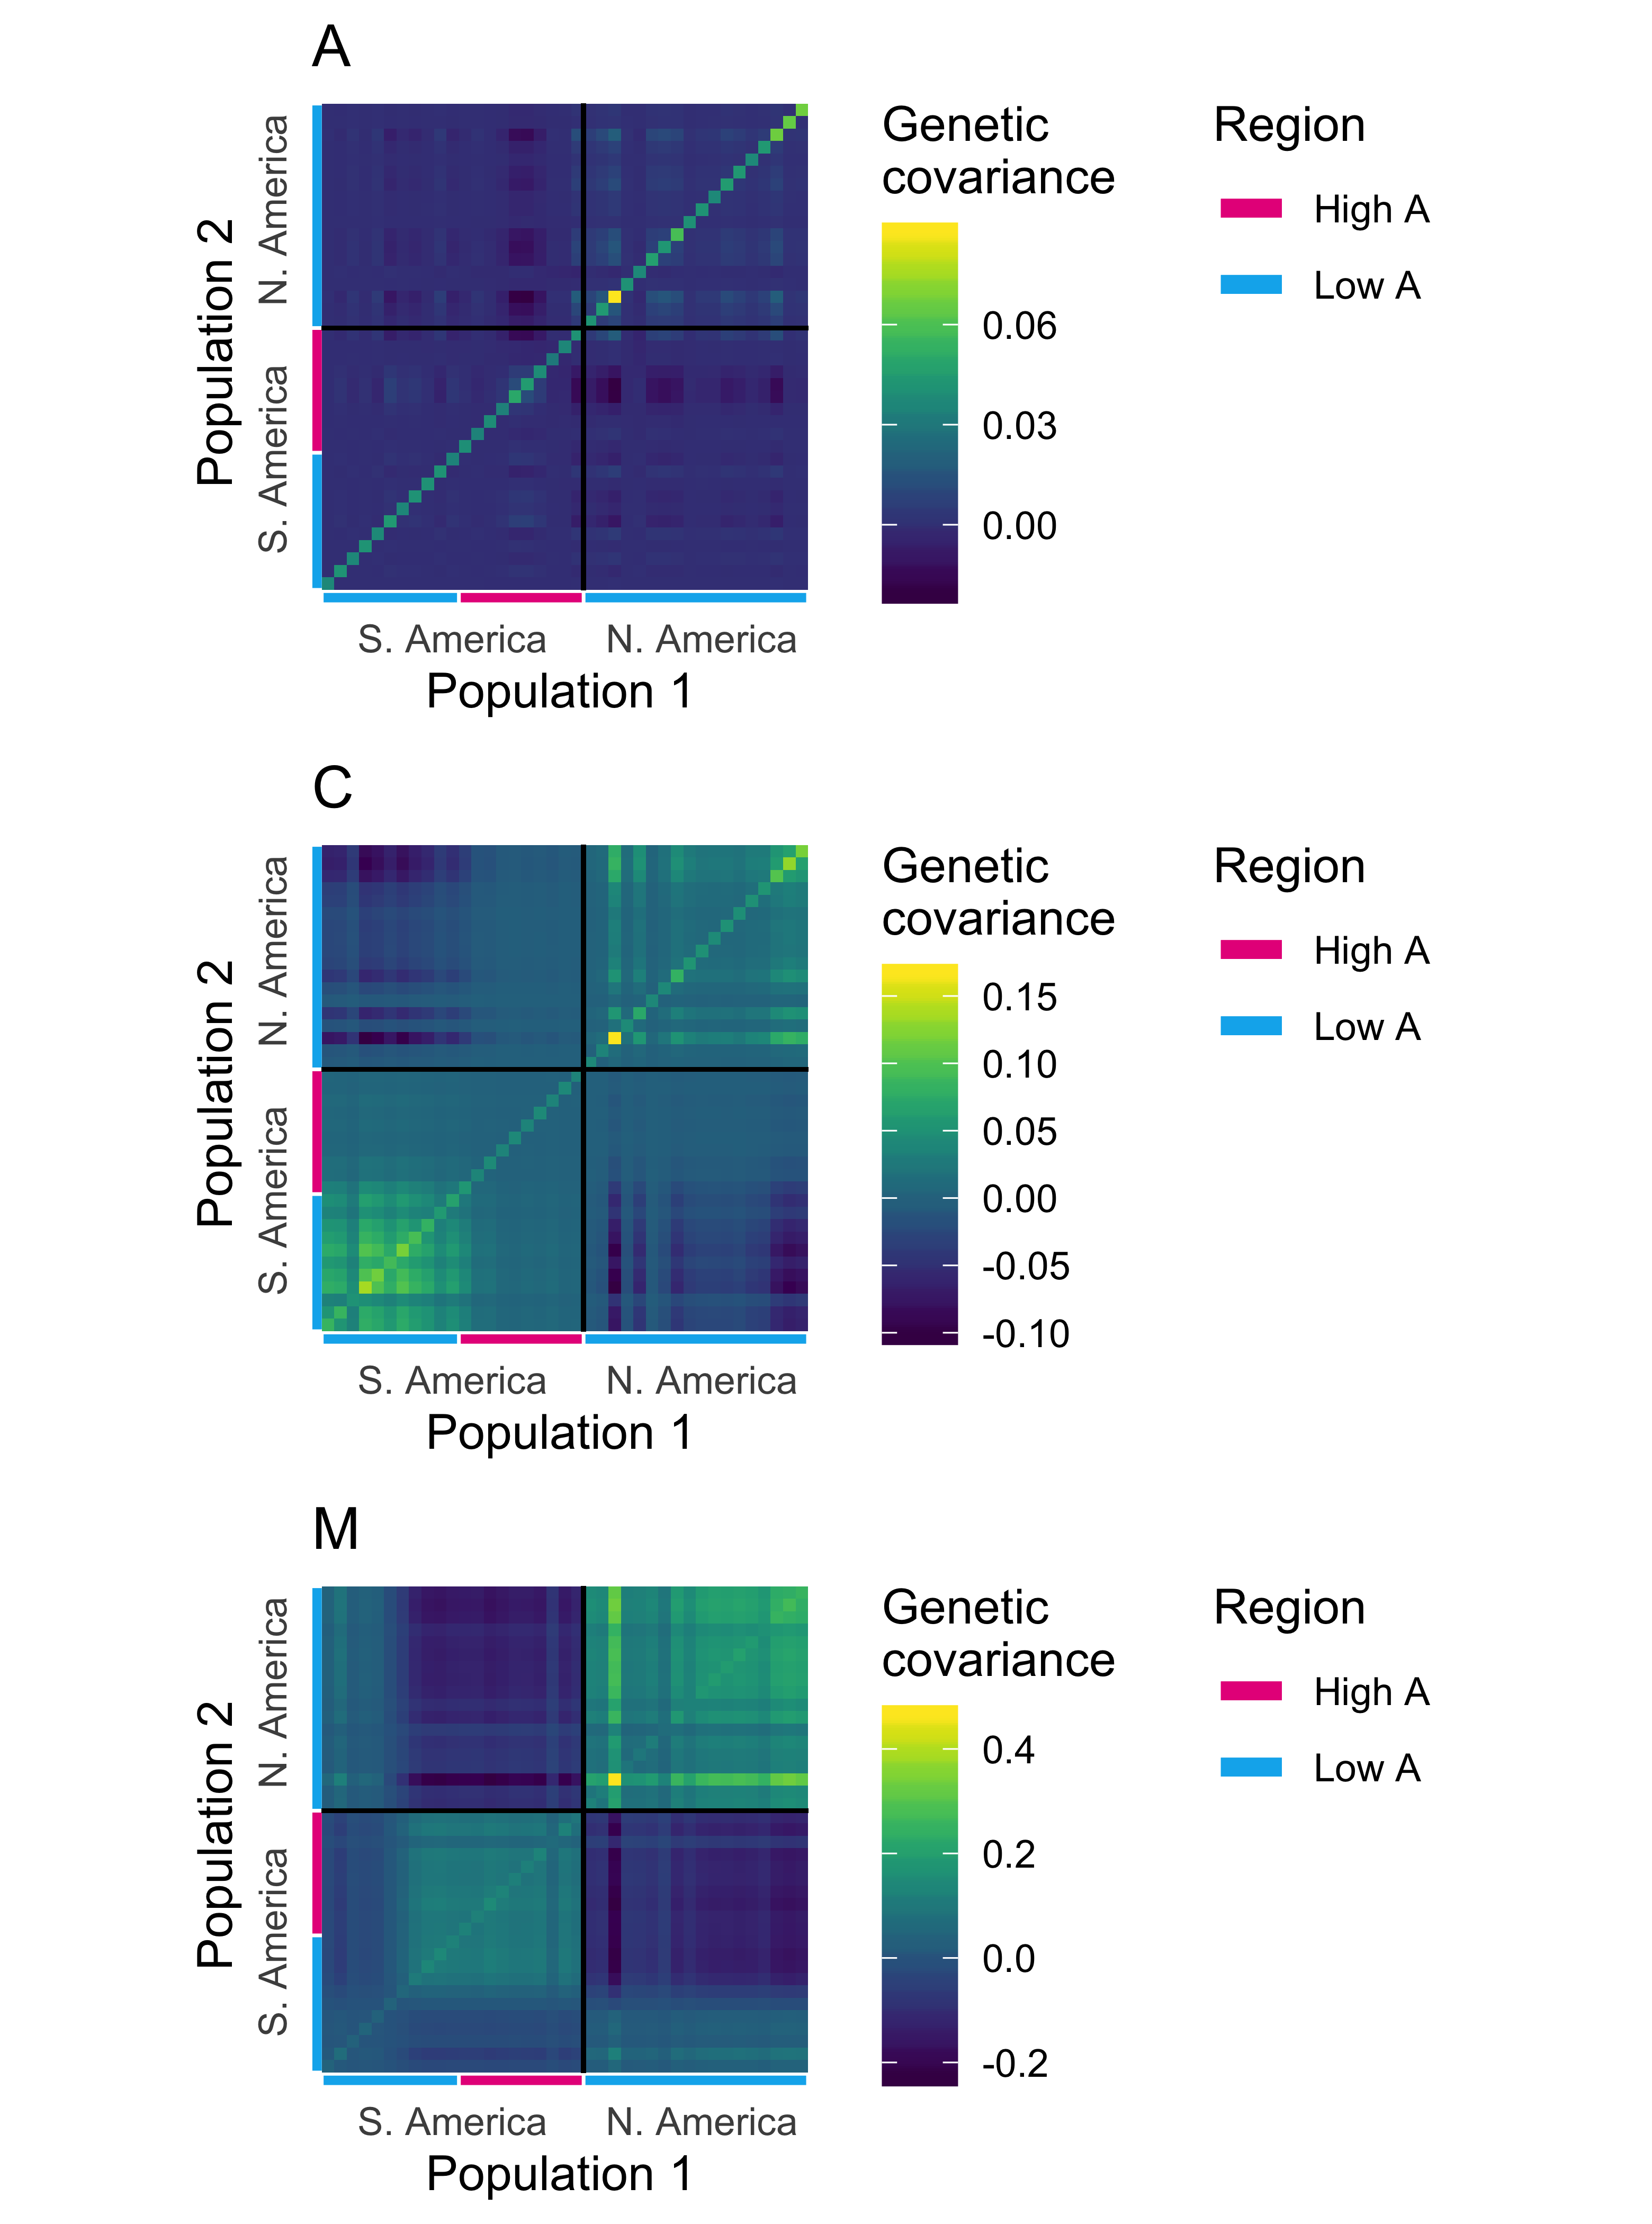
\includegraphics[width=.68\textwidth]{chapter1/figures/genetic_cov_within_ancestry.png}
\caption{\ec{\textbf{Genetic covariance within ancestry.} Genetic covariances within A (top), C (middle) and M (bottom) ancestry. Colors represent the population mean genetic covariance between individuals, and the range of values varies by ancestry (note: color bars have different scales). While kinship creates strictly positive covariances, here we observe some negative values because we can only calculate co-variation around the empirical mean combined sample allele frequency, not the true ancestral allele frequency (which is unknown).
Population mean covariances were summarised from an individual-by-individual covariance matrix generated using PCAngsd from bam files filtered to only include regions of the genome with high confidence homozygous ancestry calls for the focal ancestry (posterior \textgreater 0.8 from ancestry\_hmm). High and low A sides of each hybrid zone are defined relative to the estimated genomewide cline center}}
\label{cov_within_anc}
\end{figure}

\begin{figure}[ht]
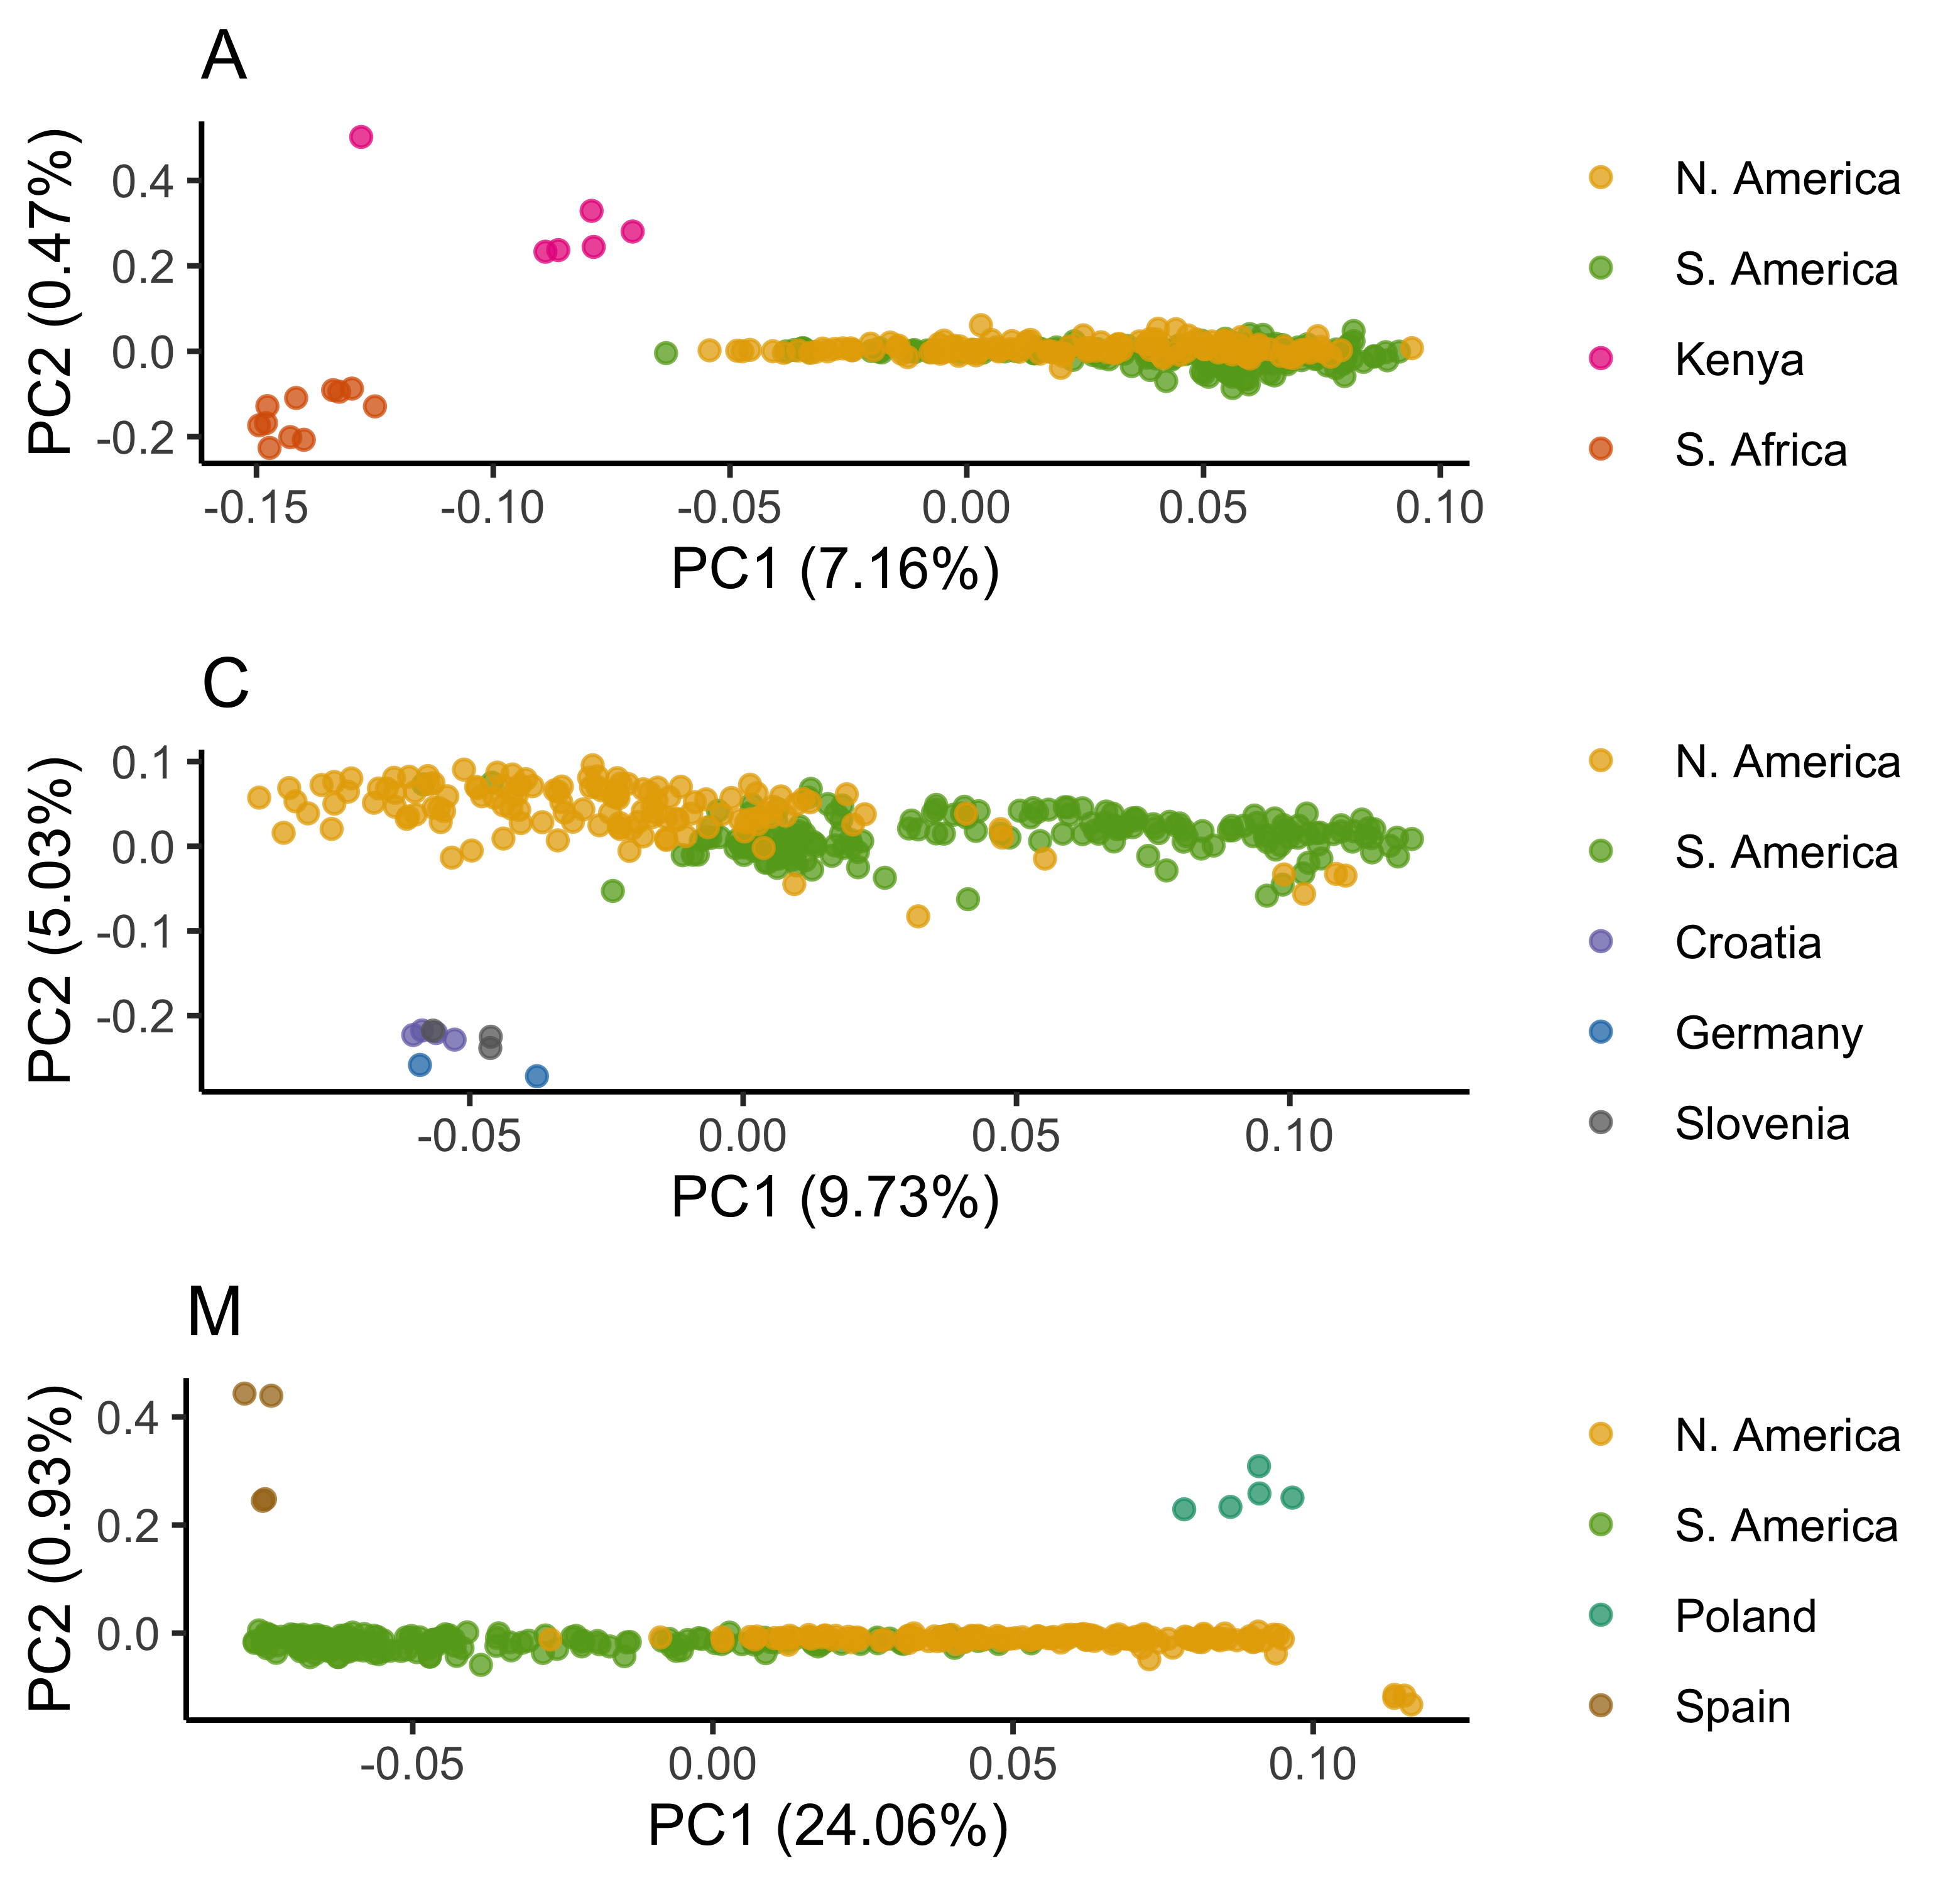
\includegraphics[width=.9\textwidth]{chapter1/figures/p_pca_by_anc.png}
\caption{\ec{\textbf{Principle components analysis of genetic variation within ancestry.} PCA analysis of A (top), C (middle) and M (bottom) ancestry. Analysis was performed using PCAngsd using all reference samples of the focal ancestry and sequence data from the hybrid zones filtered to only include regions of the genome with high confidence homozygous ancestry calls for the focal ancestry (posterior \textgreater 0.8 from ancestry\_hmm). Each bee is a point, colored by sample location. The two hybrid zones form somewhat separable clusters for European (C and M) ancestry, but not \scutellata\ (A) ancestry. The major axis of genetic diversity within M ancestry in the Americas (PC1) mirrors pre-existing population structure within Europe between \textit{Apis mellifera mellifera} (Poland) and \textit{Apis mellifera iberiensis} (Spain), two well-known honeybee subspecies that may have different historical import rates to different regions.}}
\label{pca_within_anc}
\end{figure}

\begin{figure}[ht]
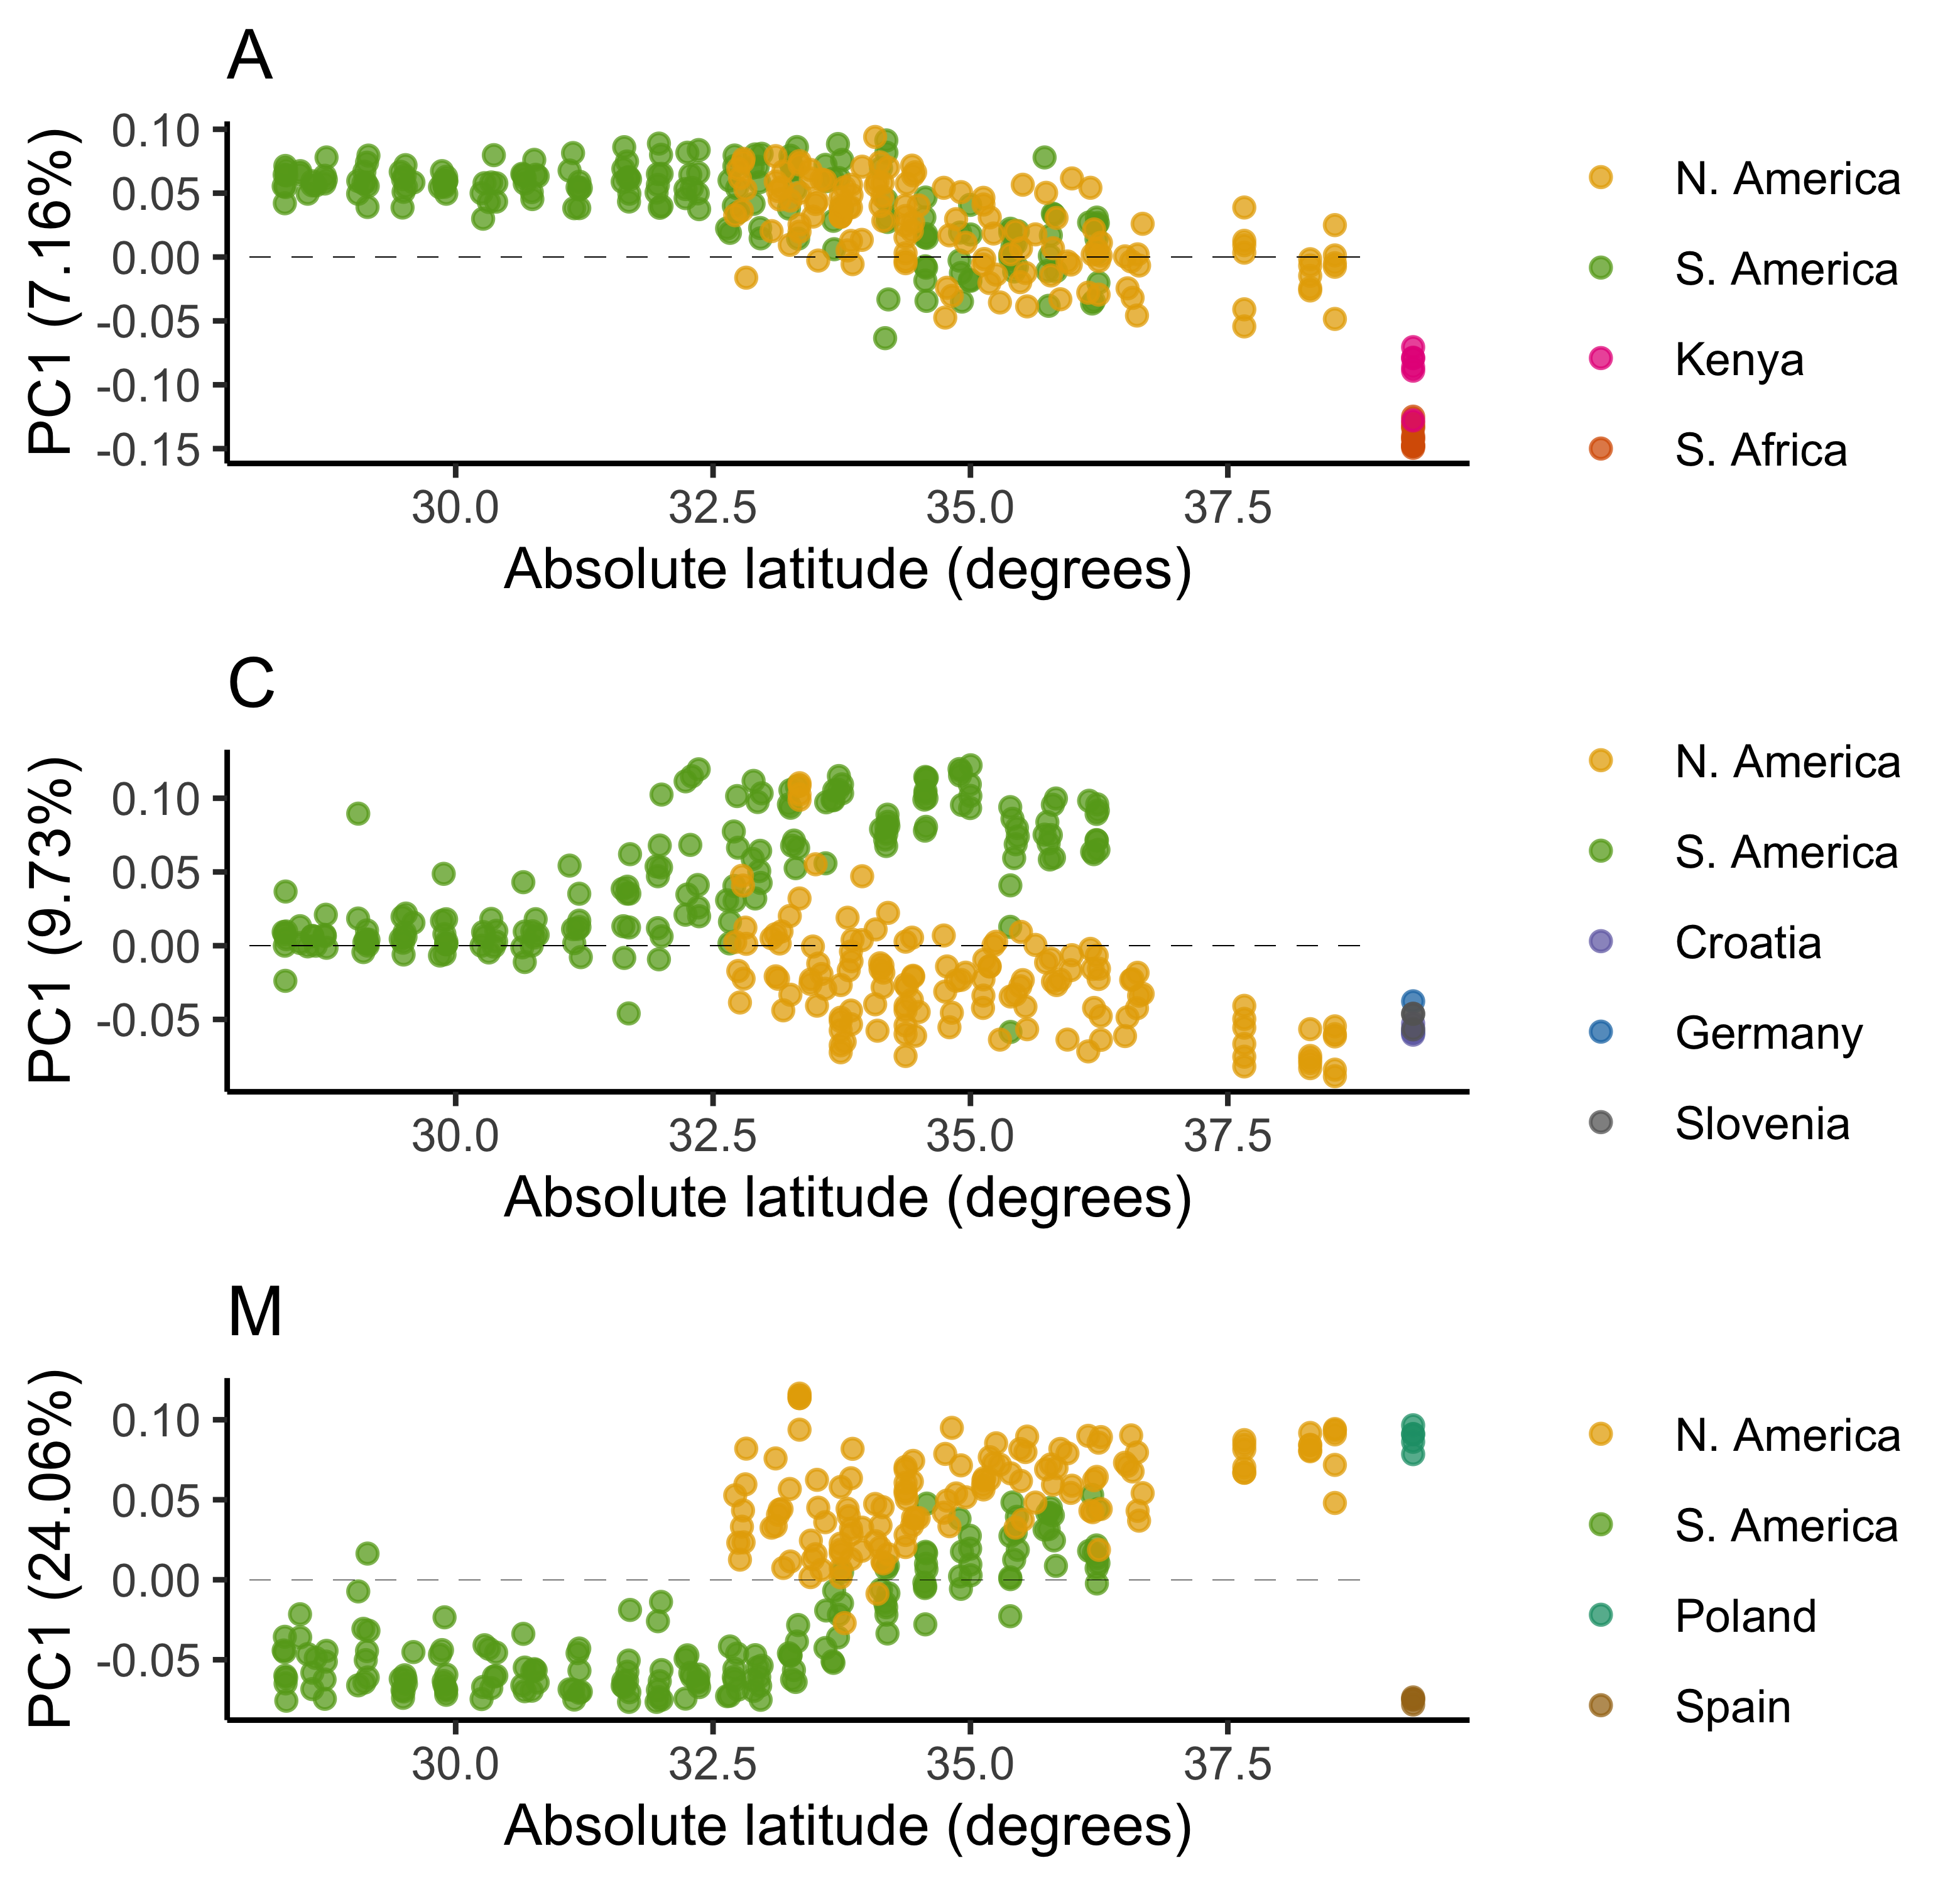
\includegraphics[width=.85\textwidth]{chapter1/figures/pc1_anc_by_lat.png}
\caption{\ec{\textbf{Genetic variation within ancestry by latitude.} Here we plot the first principal component for genetic diversity within A (top), C (middle) and M (bottom) ancestry against absolute latitude of sampling location within the hybrid zone (see Fig \ref{pca_within_anc} for original PCA). Each bee is a point and reference bees are plotted to the side (not at their actual latitude). Bees are colored by sample location. Note that bees with very low amounts of the focal ancestry (higher latitudes A ancestry or lower latitudes C ancestry) fall close to zero on PC1 (dashed line), which, despite using a method designed to account for low coverage data (PCAngsd), may simply be an artifact of low information per individual bee for genetic diversity within a low-frequency ancestry. A ancestry shows very little population structure along PC1 by continent or latitude. C is the dominant ancestry at higher latitudes in both zones and shows greater separation between the two ends of the zones (higher absolute latitude for both) than within South America. M ancestry at lower latitudes in South America is more similar to \textit{Apis mellifera iberiensis} (Spain) than M ancestry elsewhere in the Americas.}}
\label{pc1_anc_by_lat}
\end{figure}

\begin{figure}[ht]
%\begin{center}
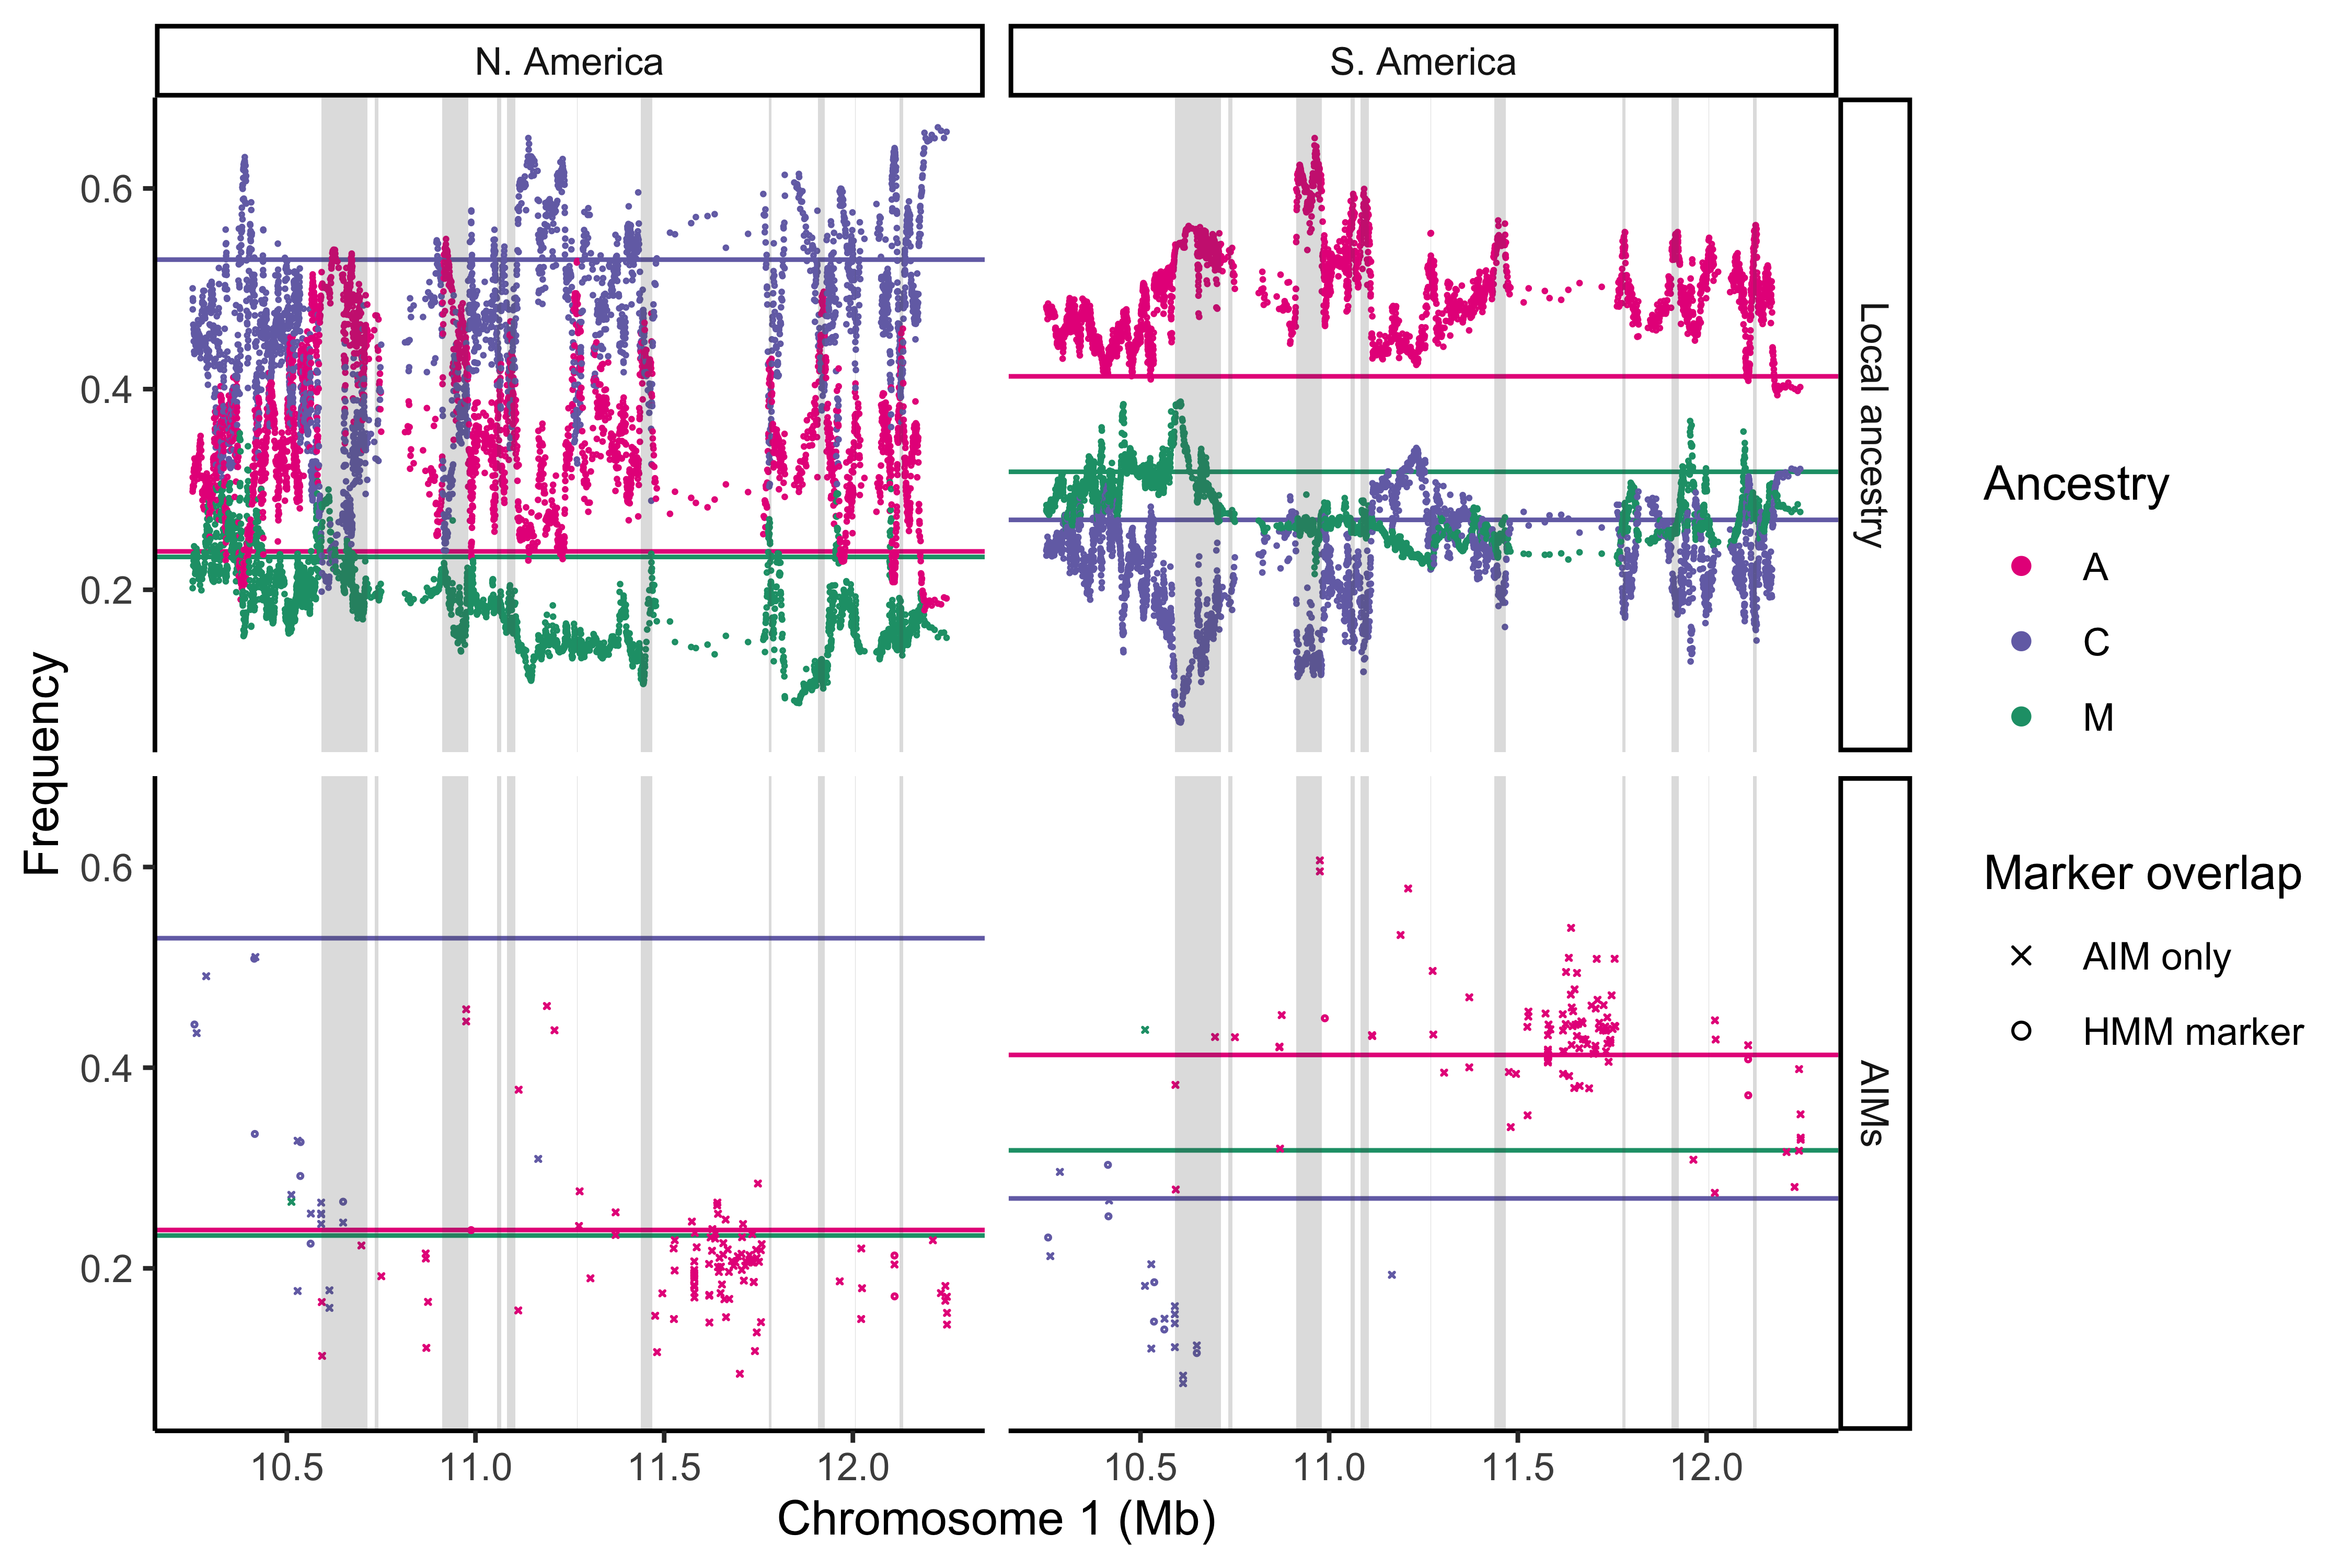
\includegraphics[width = \textwidth]{chapter1/figures/ACM_frequency_plot_AR_CA_FDR_chr1_outlier2.png}
%\end{center}
\caption{ \textbf{Ancestry and AIM frequencies for high shared A outliers on chr1.} Zoomed-in view of the region on chromosome 1 with a cluster of high \A\ ancestry peaks in both North America (left) and South America (right), with shared outlier regions meeting a 10\% FDR for high \A\ ancestry on both continents shaded in grey. (Top) \ahb{\textit{Scutellata}} (A), western European (M) and eastern European (C) local ancestry estimates at each HMM marker. (Bottom) Mean frequency of ancestry informative markers AIMs (see methods), most of which were not included in the ancestry\_hmm inference (‘AIM only') due to thinning.}
\label{ACM_chr1_outlier_AIMs}
\end{figure}

\begin{figure}[ht]
%\begin{center}
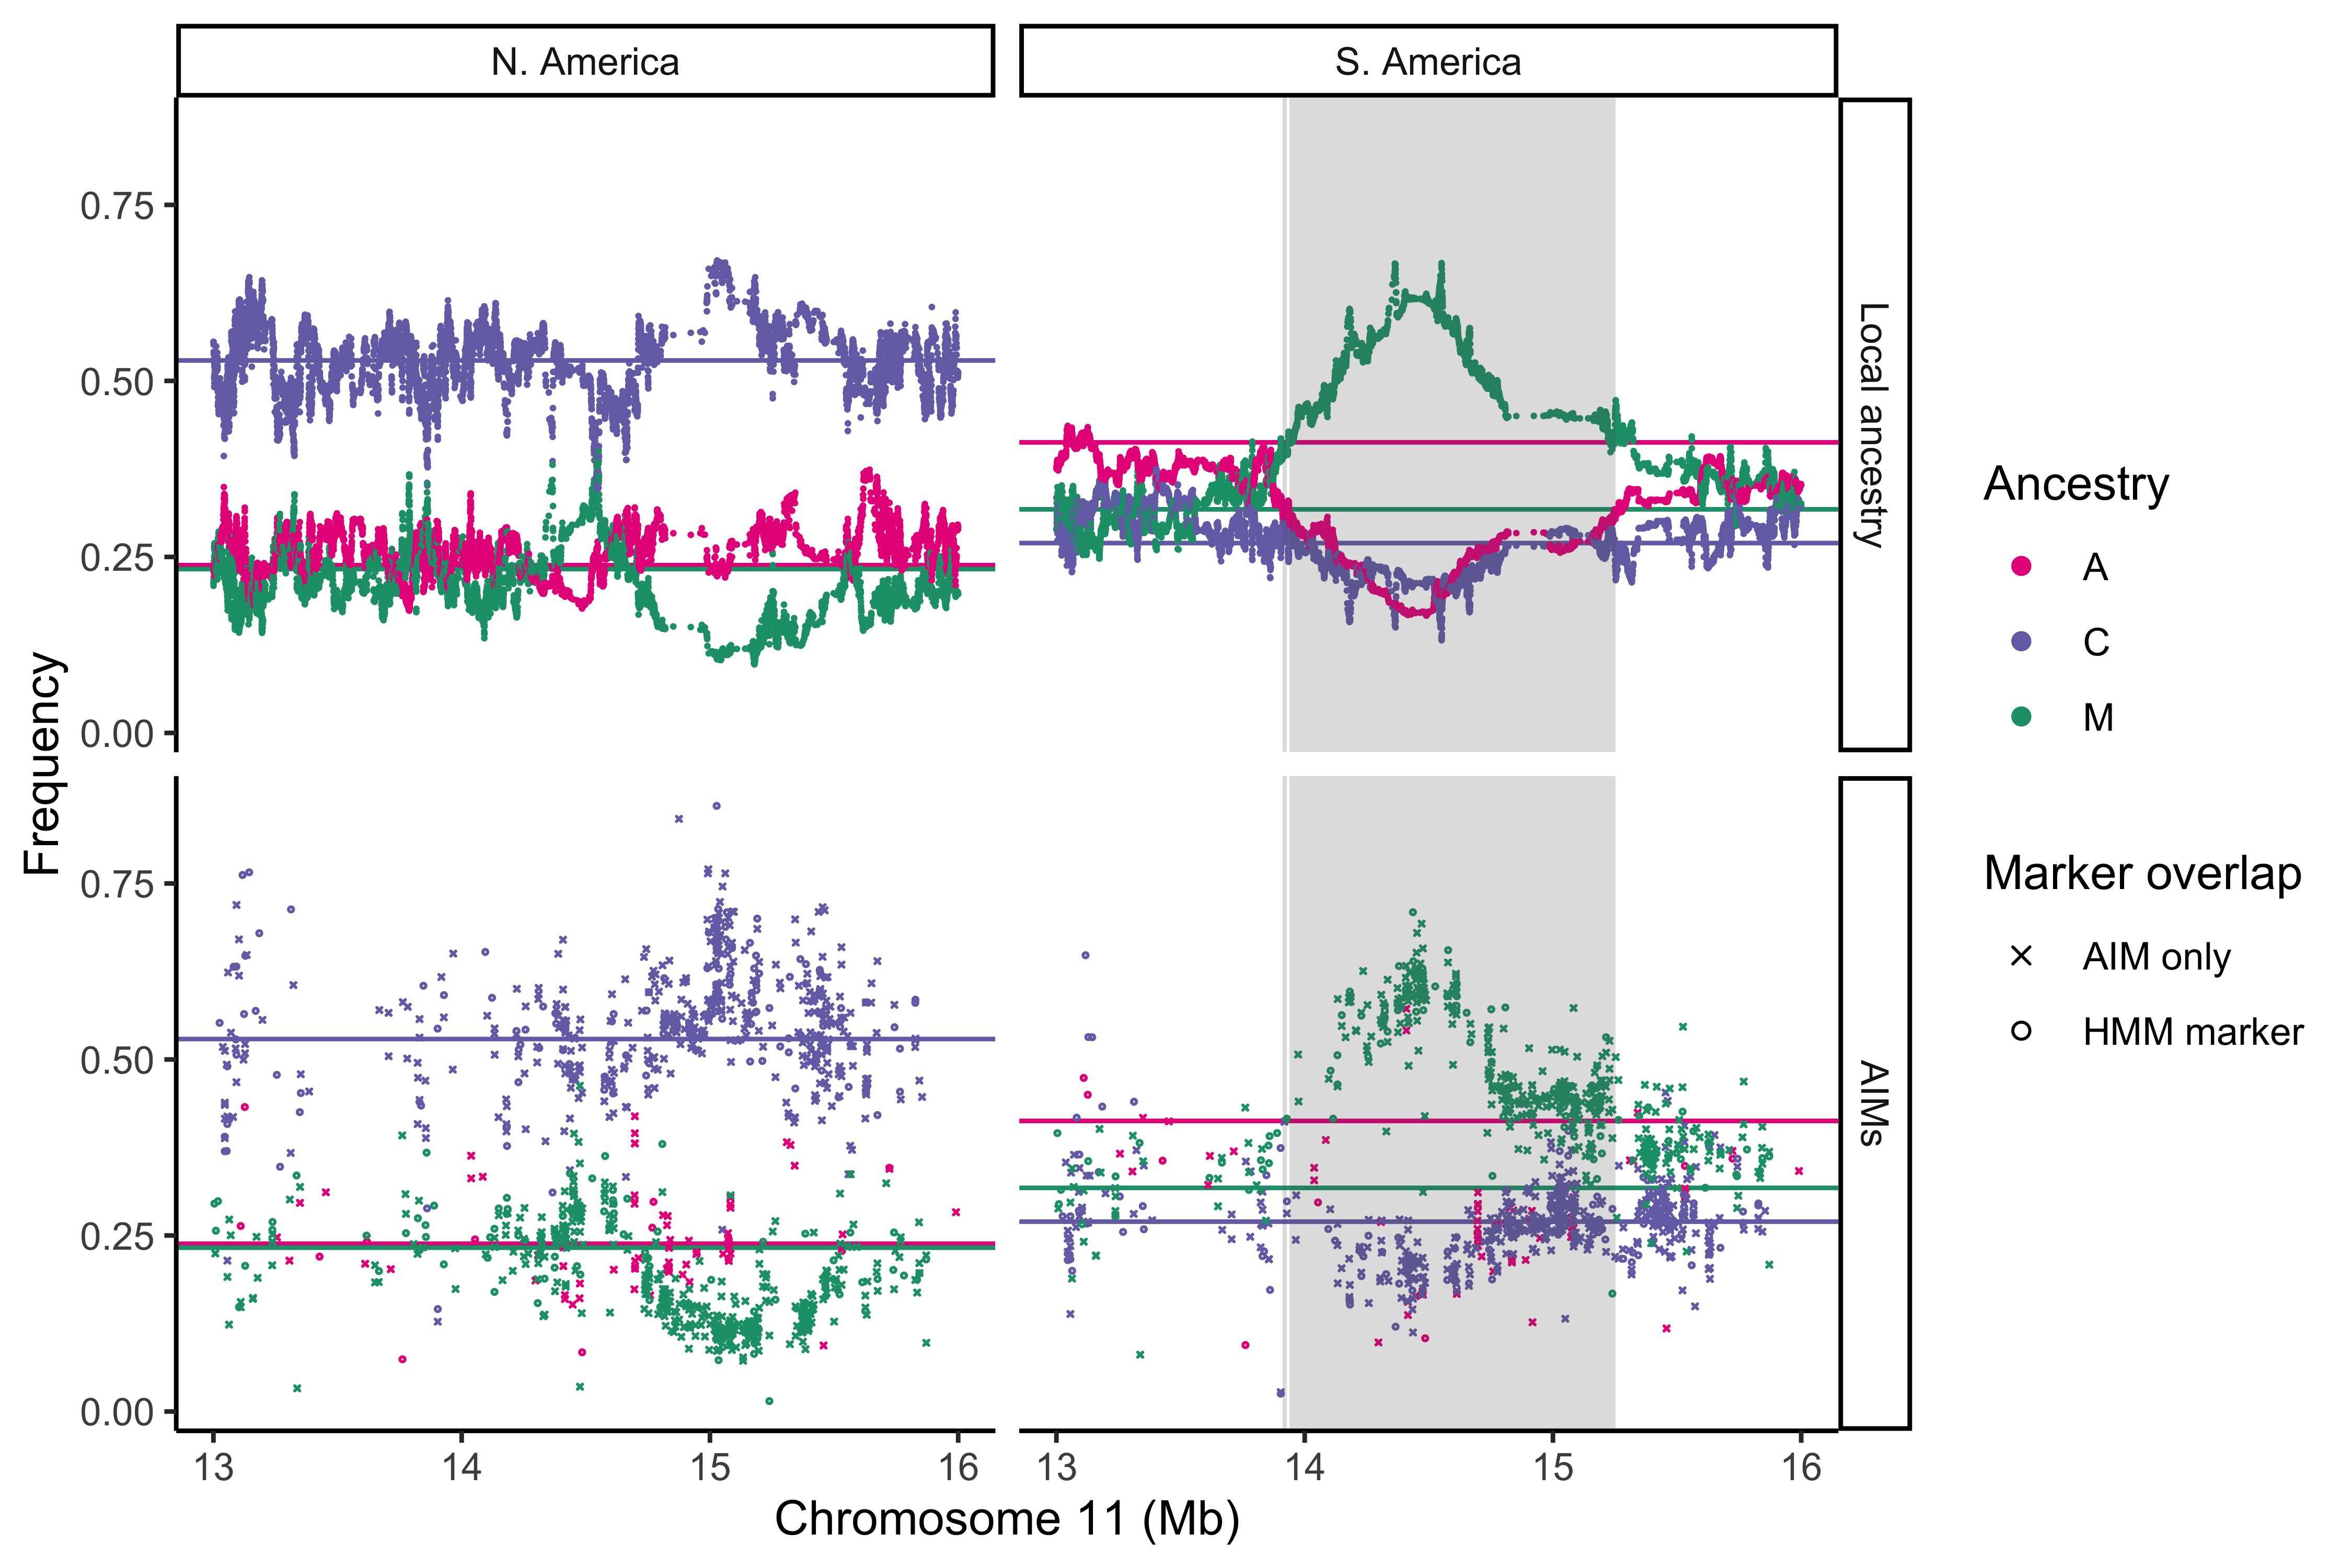
\includegraphics[width = \textwidth]{chapter1/figures/ACM_frequency_plot_AR_CA_FDR_chr11_outlier2.png}
%\end{center}
 \caption{ \textbf{Ancestry and AIM frequencies for low A outlier region on chr11.} Zoomed-in view of the 1.4Mb region on chromosome 11 with high western European ancestry (M) in South America (right) but not in North America (left), with the outlier region meeting 10\% FDR highlighted in grey. (Top) \ahb{\textit{Scutellata}} (A), western European (M) and eastern European (C) local ancestry estimates at each HMM marker. (Bottom) Mean frequency of ancestry informative markers AIMs (see methods), most of which were not included in the ancestry\_hmm inference (‘AIM only') due to thinning.}
\label{ACM_chr11_outlier_AIMs}
\end{figure}


\begin{figure}[ht]
%\begin{center}
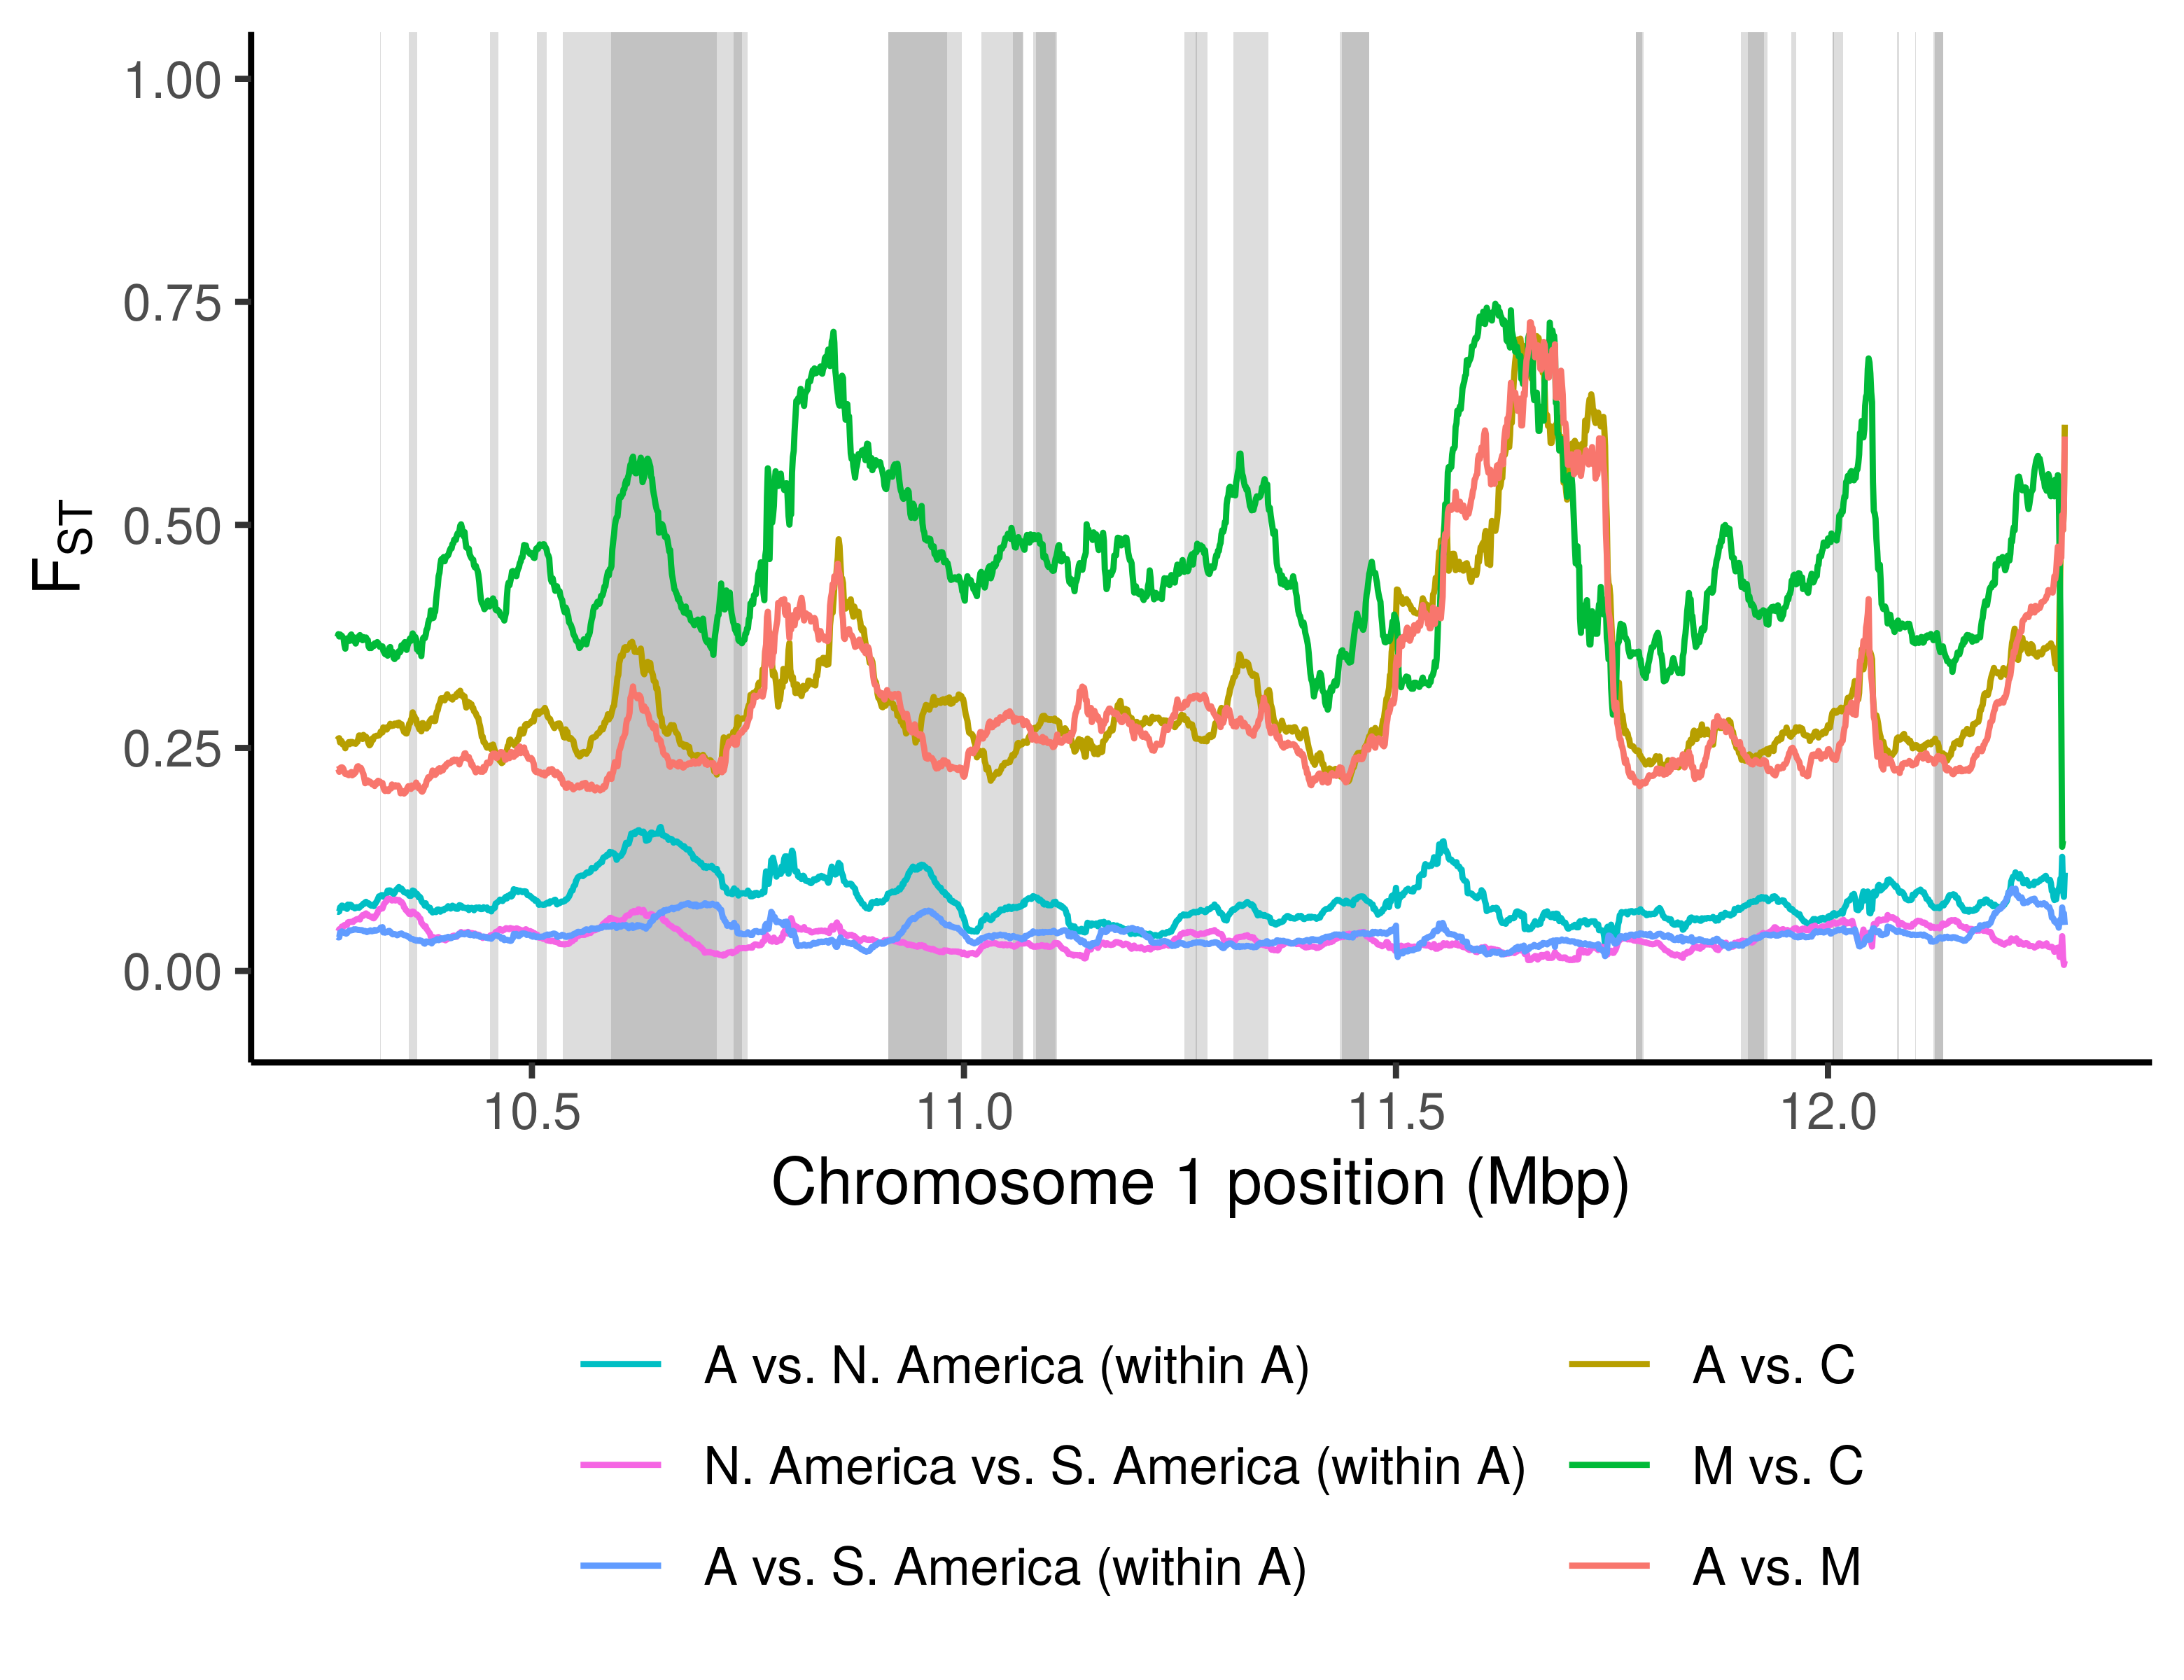
\includegraphics[width = \textwidth]{chapter1/figures/Fst_across_chr1_outliers.png}
%\end{center}
 \caption{ \textbf{Differentiation across shared high A outliers on chr1.} F\textsubscript{ST} across the region on chromosome 1 with shared high \A\ ancestry outliers. Outlier regions meeting a 10\% FDR in both hybrid zones are highlighted in darker grey, while those meeting a 10\% FDR in only one hybrid zone are highlighted in lighter grey. Per-SNP F\textsubscript{ST} is averaged within sliding 50kb windows. In addition to the three ancestry reference panels (A, C, \& M), we include contrasts for the subset of individuals in each hybrid zone with high-confidence homozygous A ancestry.}
\label{fst_chr1_A_outlier}
\end{figure}

\begin{figure}[ht]
%\begin{center}
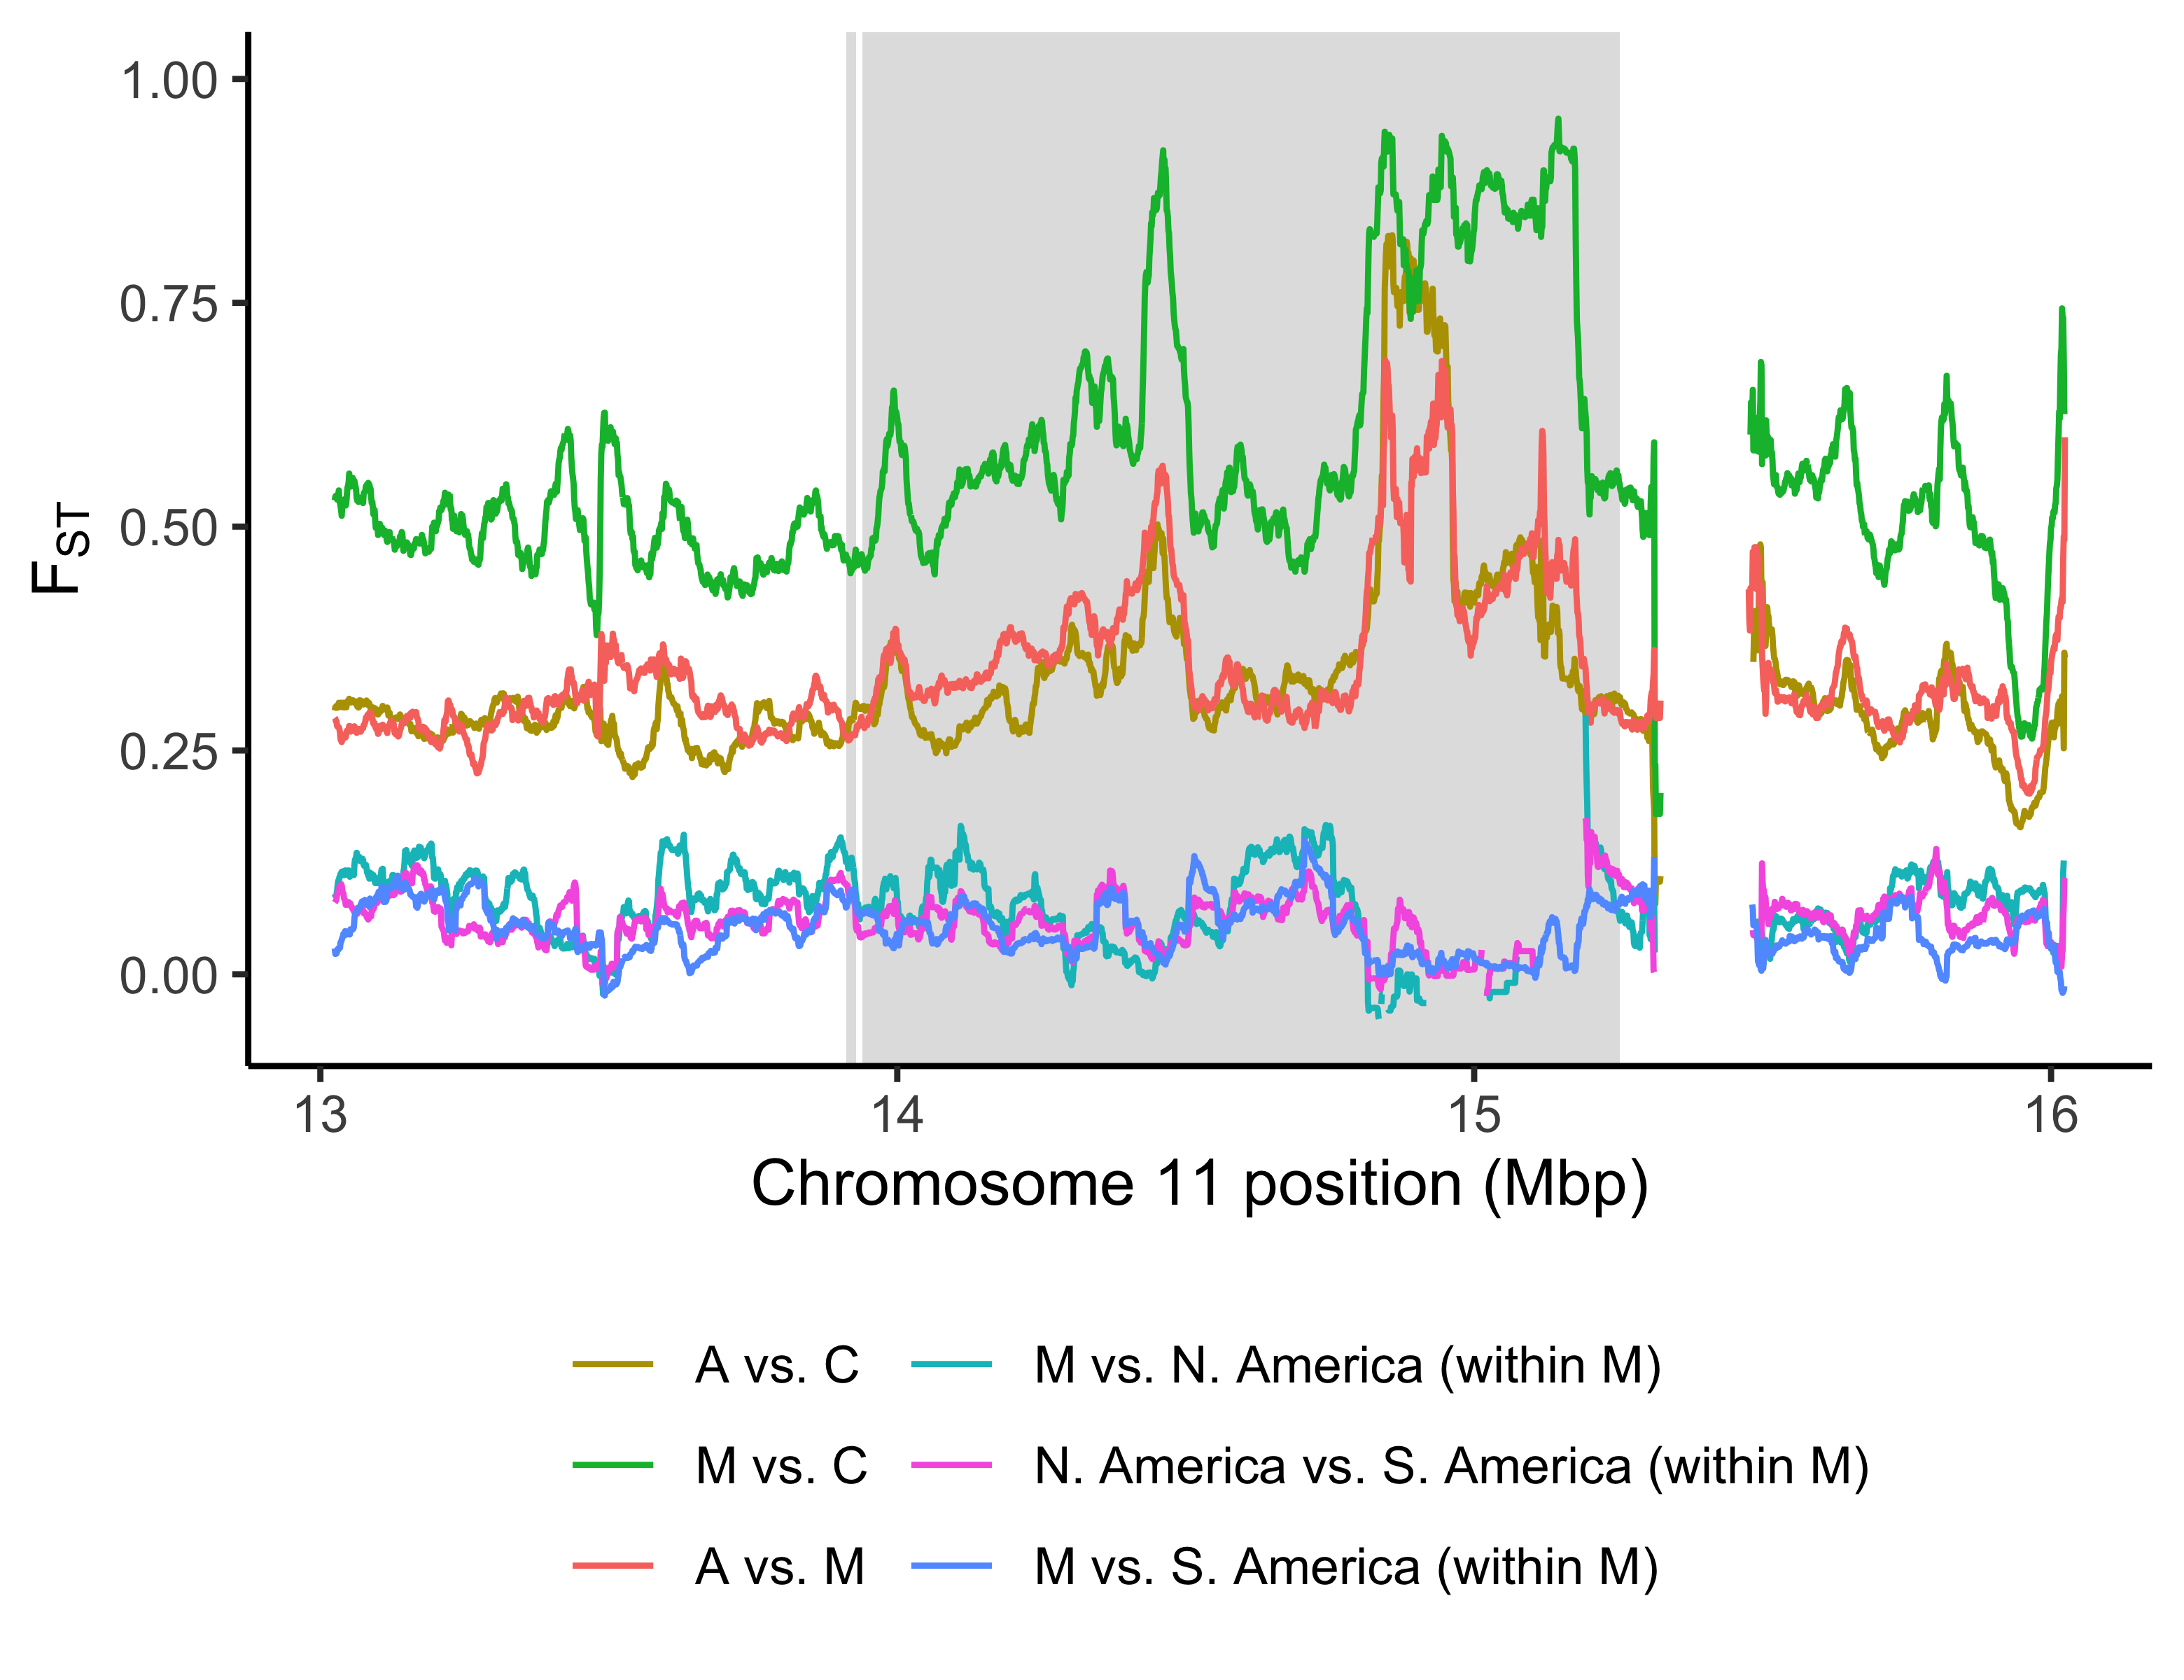
\includegraphics[width = \textwidth]{chapter1/figures/Fst_across_chr11_highA_outlier.png}
%\end{center}
 \caption{ \textbf{Differentiation across shared high A outliers on chr11.} F\textsubscript{ST} across the region on chromosome 11 with shared high \A\ ancestry outliers. Outlier regions meeting a 10\% FDR in both hybrid zones are highlighted in darker grey, while those meeting a 10\% FDR in only one hybrid zone are highlighted in lighter grey. Per-SNP F\textsubscript{ST} is averaged within sliding 50kb windows. In addition to the three ancestry reference panels (A, C, \& M), we include contrasts for the subset of individuals in each hybrid zone with high-confidence homozygous A ancestry.}
\label{fst_chr11_A_outlier}
\end{figure}

\begin{figure}[ht]
%\begin{center}
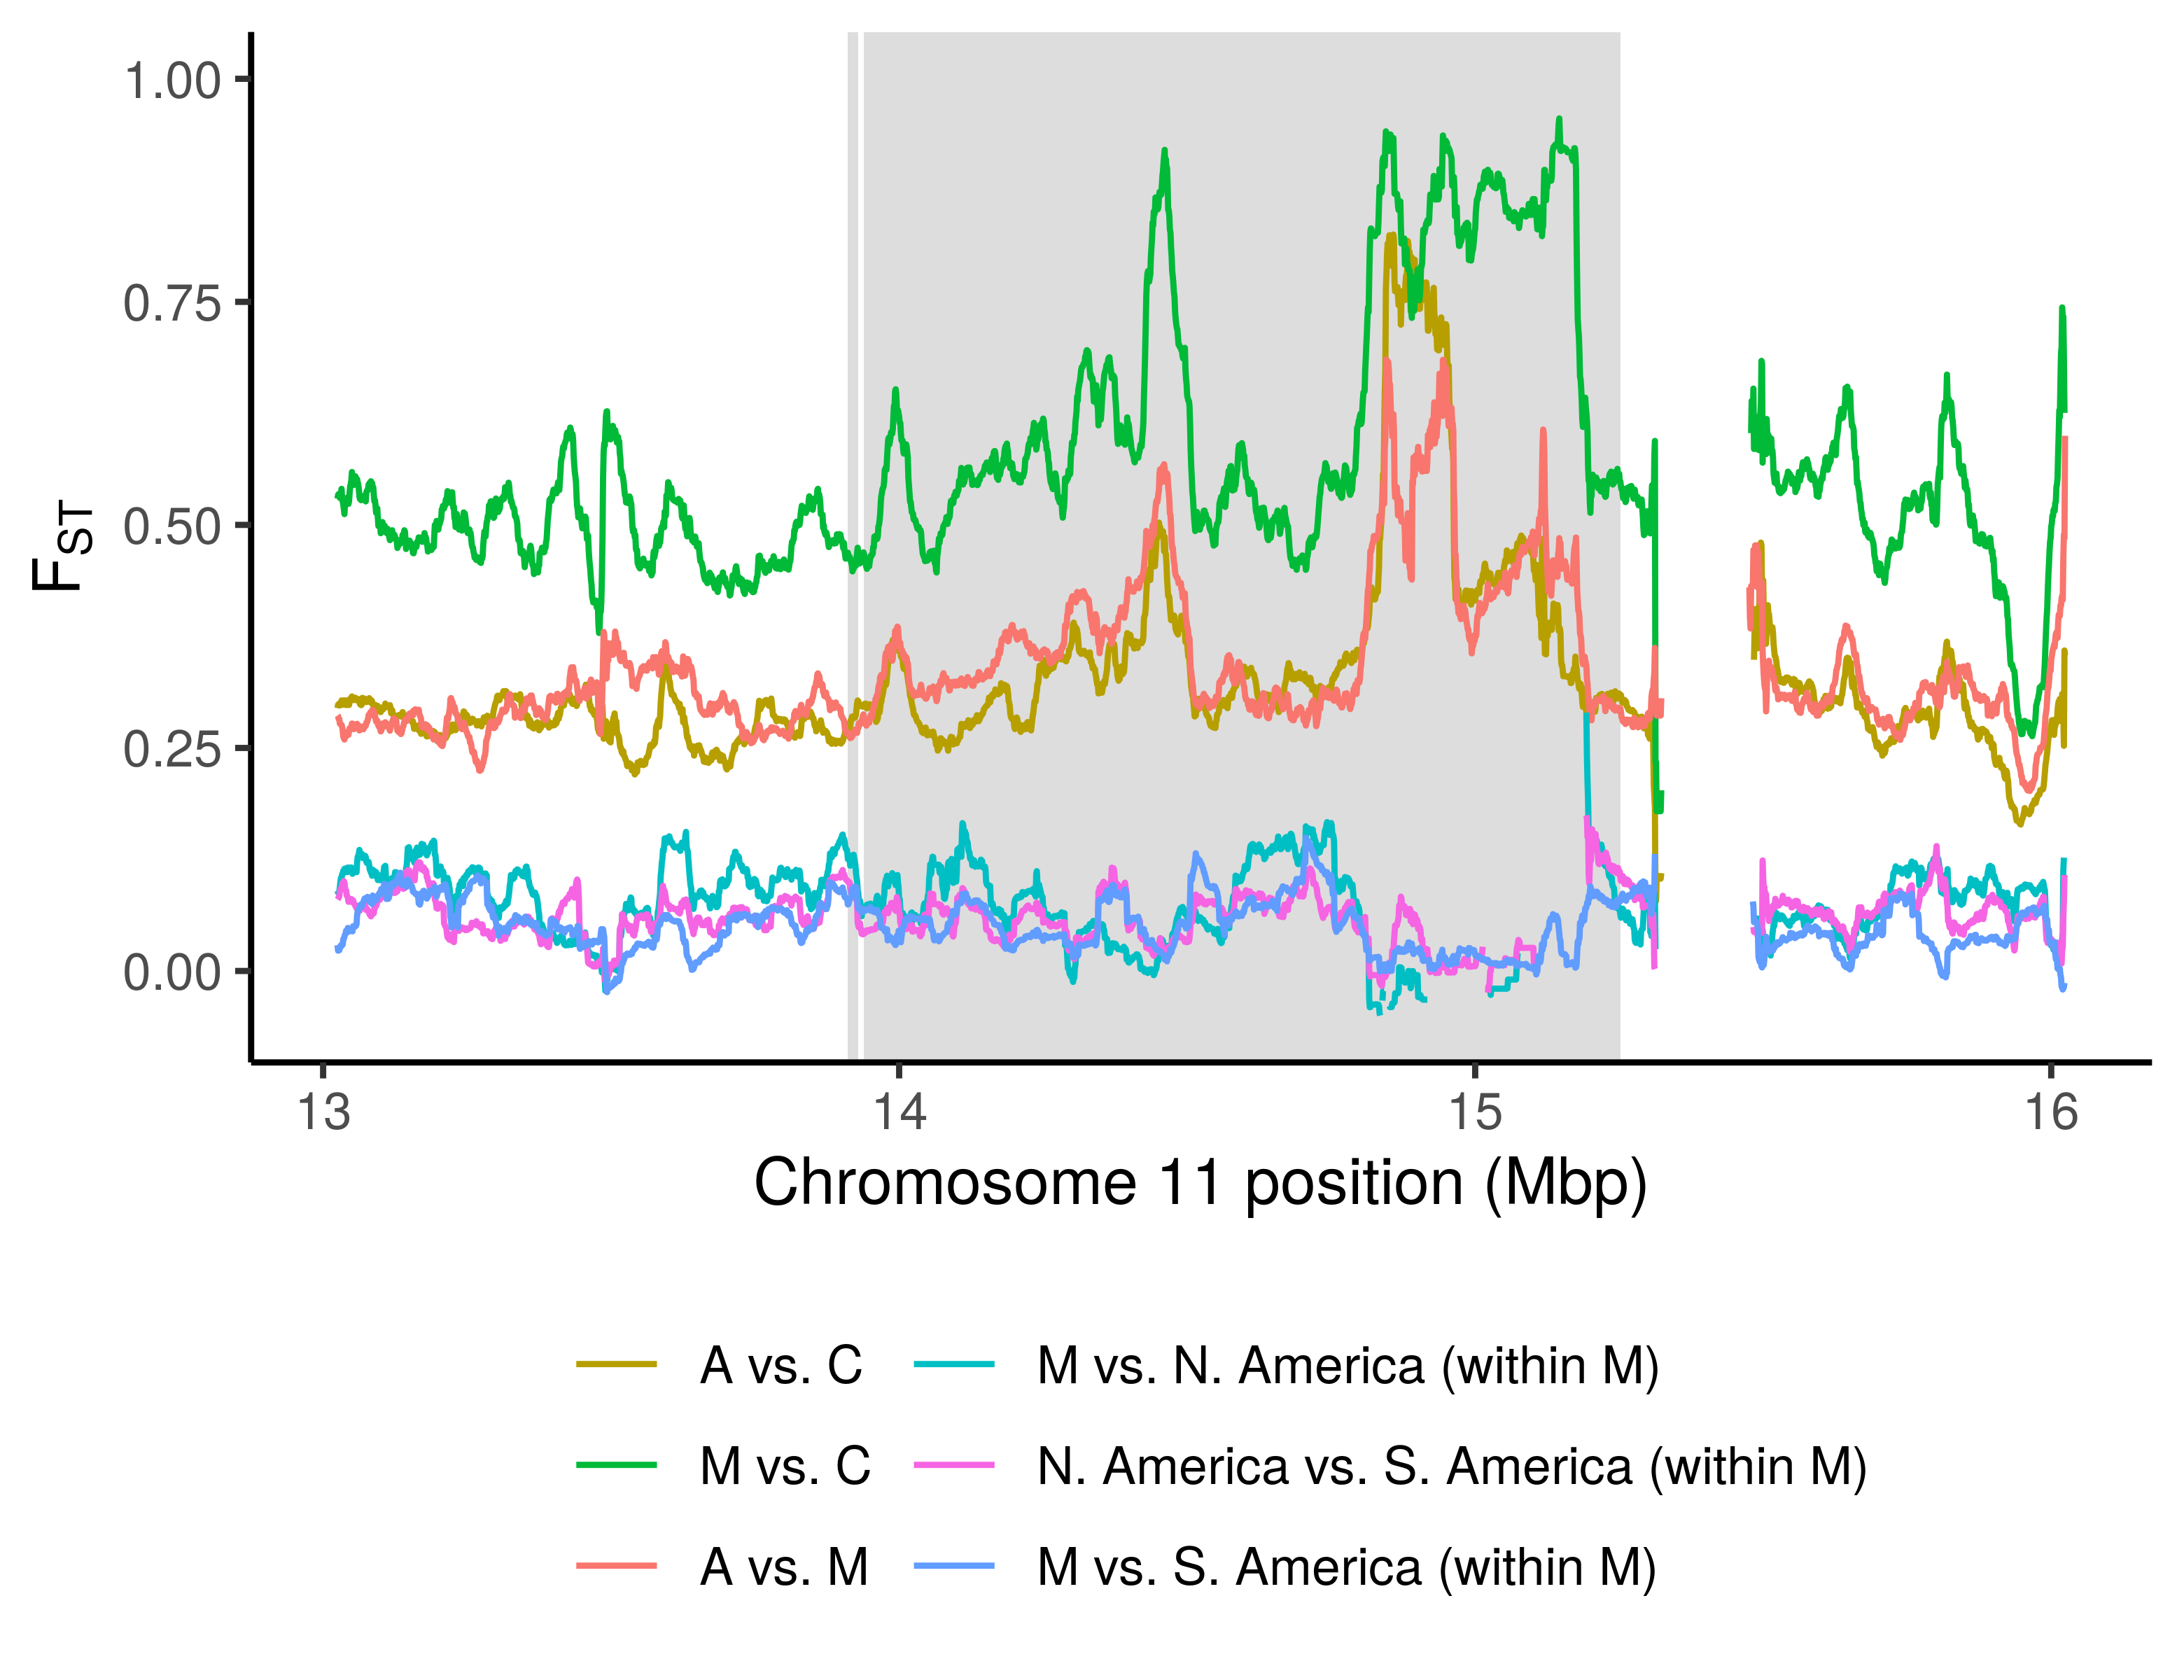
\includegraphics[width = \textwidth]{chapter1/figures/Fst_across_chr11_highM_outlier.png}
%\end{center}
 \caption{ \textbf{Differentiation across low A outlier region on chr11.} F\textsubscript{ST} across the 1.4Mb region on chromosome 11 with high western European ancestry (M) in South America but not in North America (left), with the outlier region meeting 10\% FDR highlighted in grey. Per-SNP F\textsubscript{ST} is averaged within sliding 50kb windows. In addition to the three ancestry reference panels (A, C, \& M), we include contrasts for the subset of individuals in each hybrid zone with high-confidence homozygous M ancestry. Windows are dropped if fewer than 10 SNPs have 2 individuals with data, which produces gaps in the contrasts with N. American M ancestry because this hybrid zone does not have elevated M ancestry in this region and at many SNPs very few individuals have high-confidence homozygous M ancestry. Top peaks in M vs. C, M vs. A, and C vs. A contrasts seen within this region reach the 99.5, 98.0, and 99.8 percentiles (respectively) for 50kb windows genome-wide.}
\label{fst_chr11_M_outlier}
\end{figure}

\begin{figure}[ht]
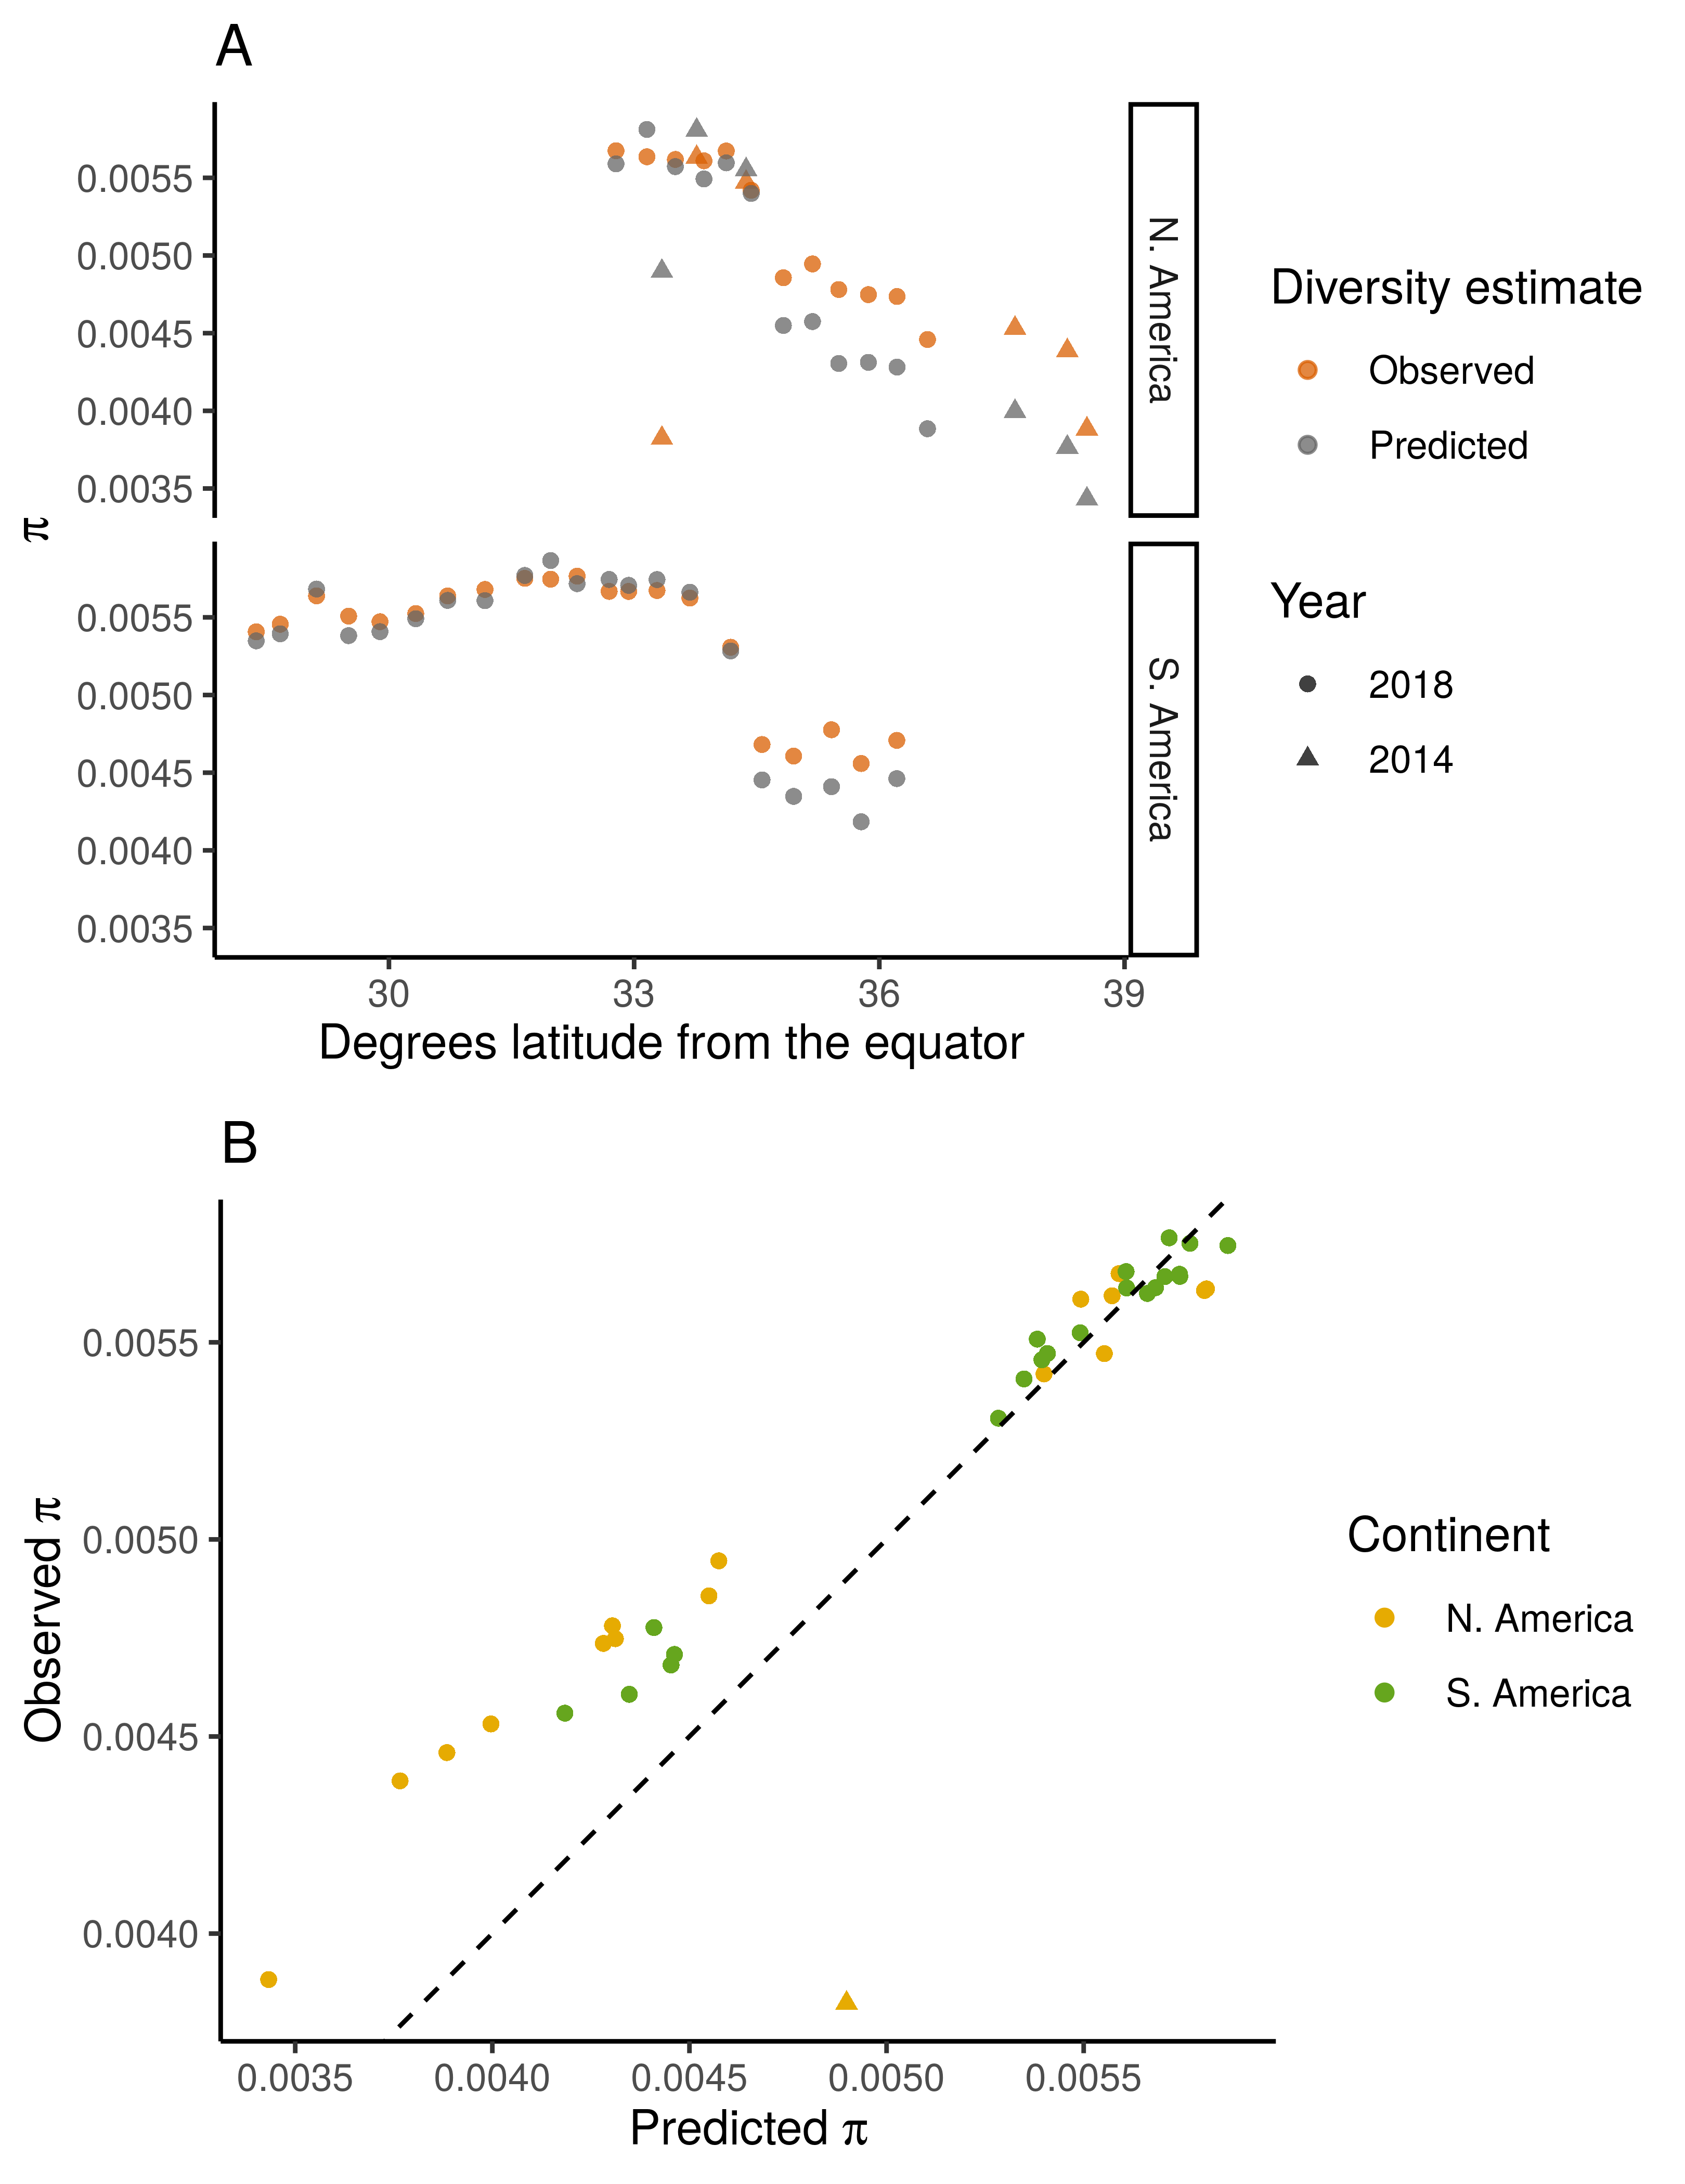
\includegraphics[width=.8\textwidth]{chapter1/figures/pi_observed_and_predicted_from_admixture.png}
\caption{ \textbf{Comparison of observed and predicted diversity.} (A) Observed and predicted allelic diversity ($\pi$) for each population across latitude. To predict $\pi$ for a specific population, we calculated the expected allele frequency based on a mixture of A, C, and M reference population allele frequencies, weighted by the population's estimated admixture fractions of these three ancestries. (B) Plot of predicted vs. observed $\pi$ for each population for direct comparison to the 1-to-1 line (dashed). Avalon (California 2014, marked as a triangle) is a clear outlier, with low diversity for its admixture fraction.}
\label{pred_vs_obs_pi}
\end{figure}

\begin{figure}[ht]
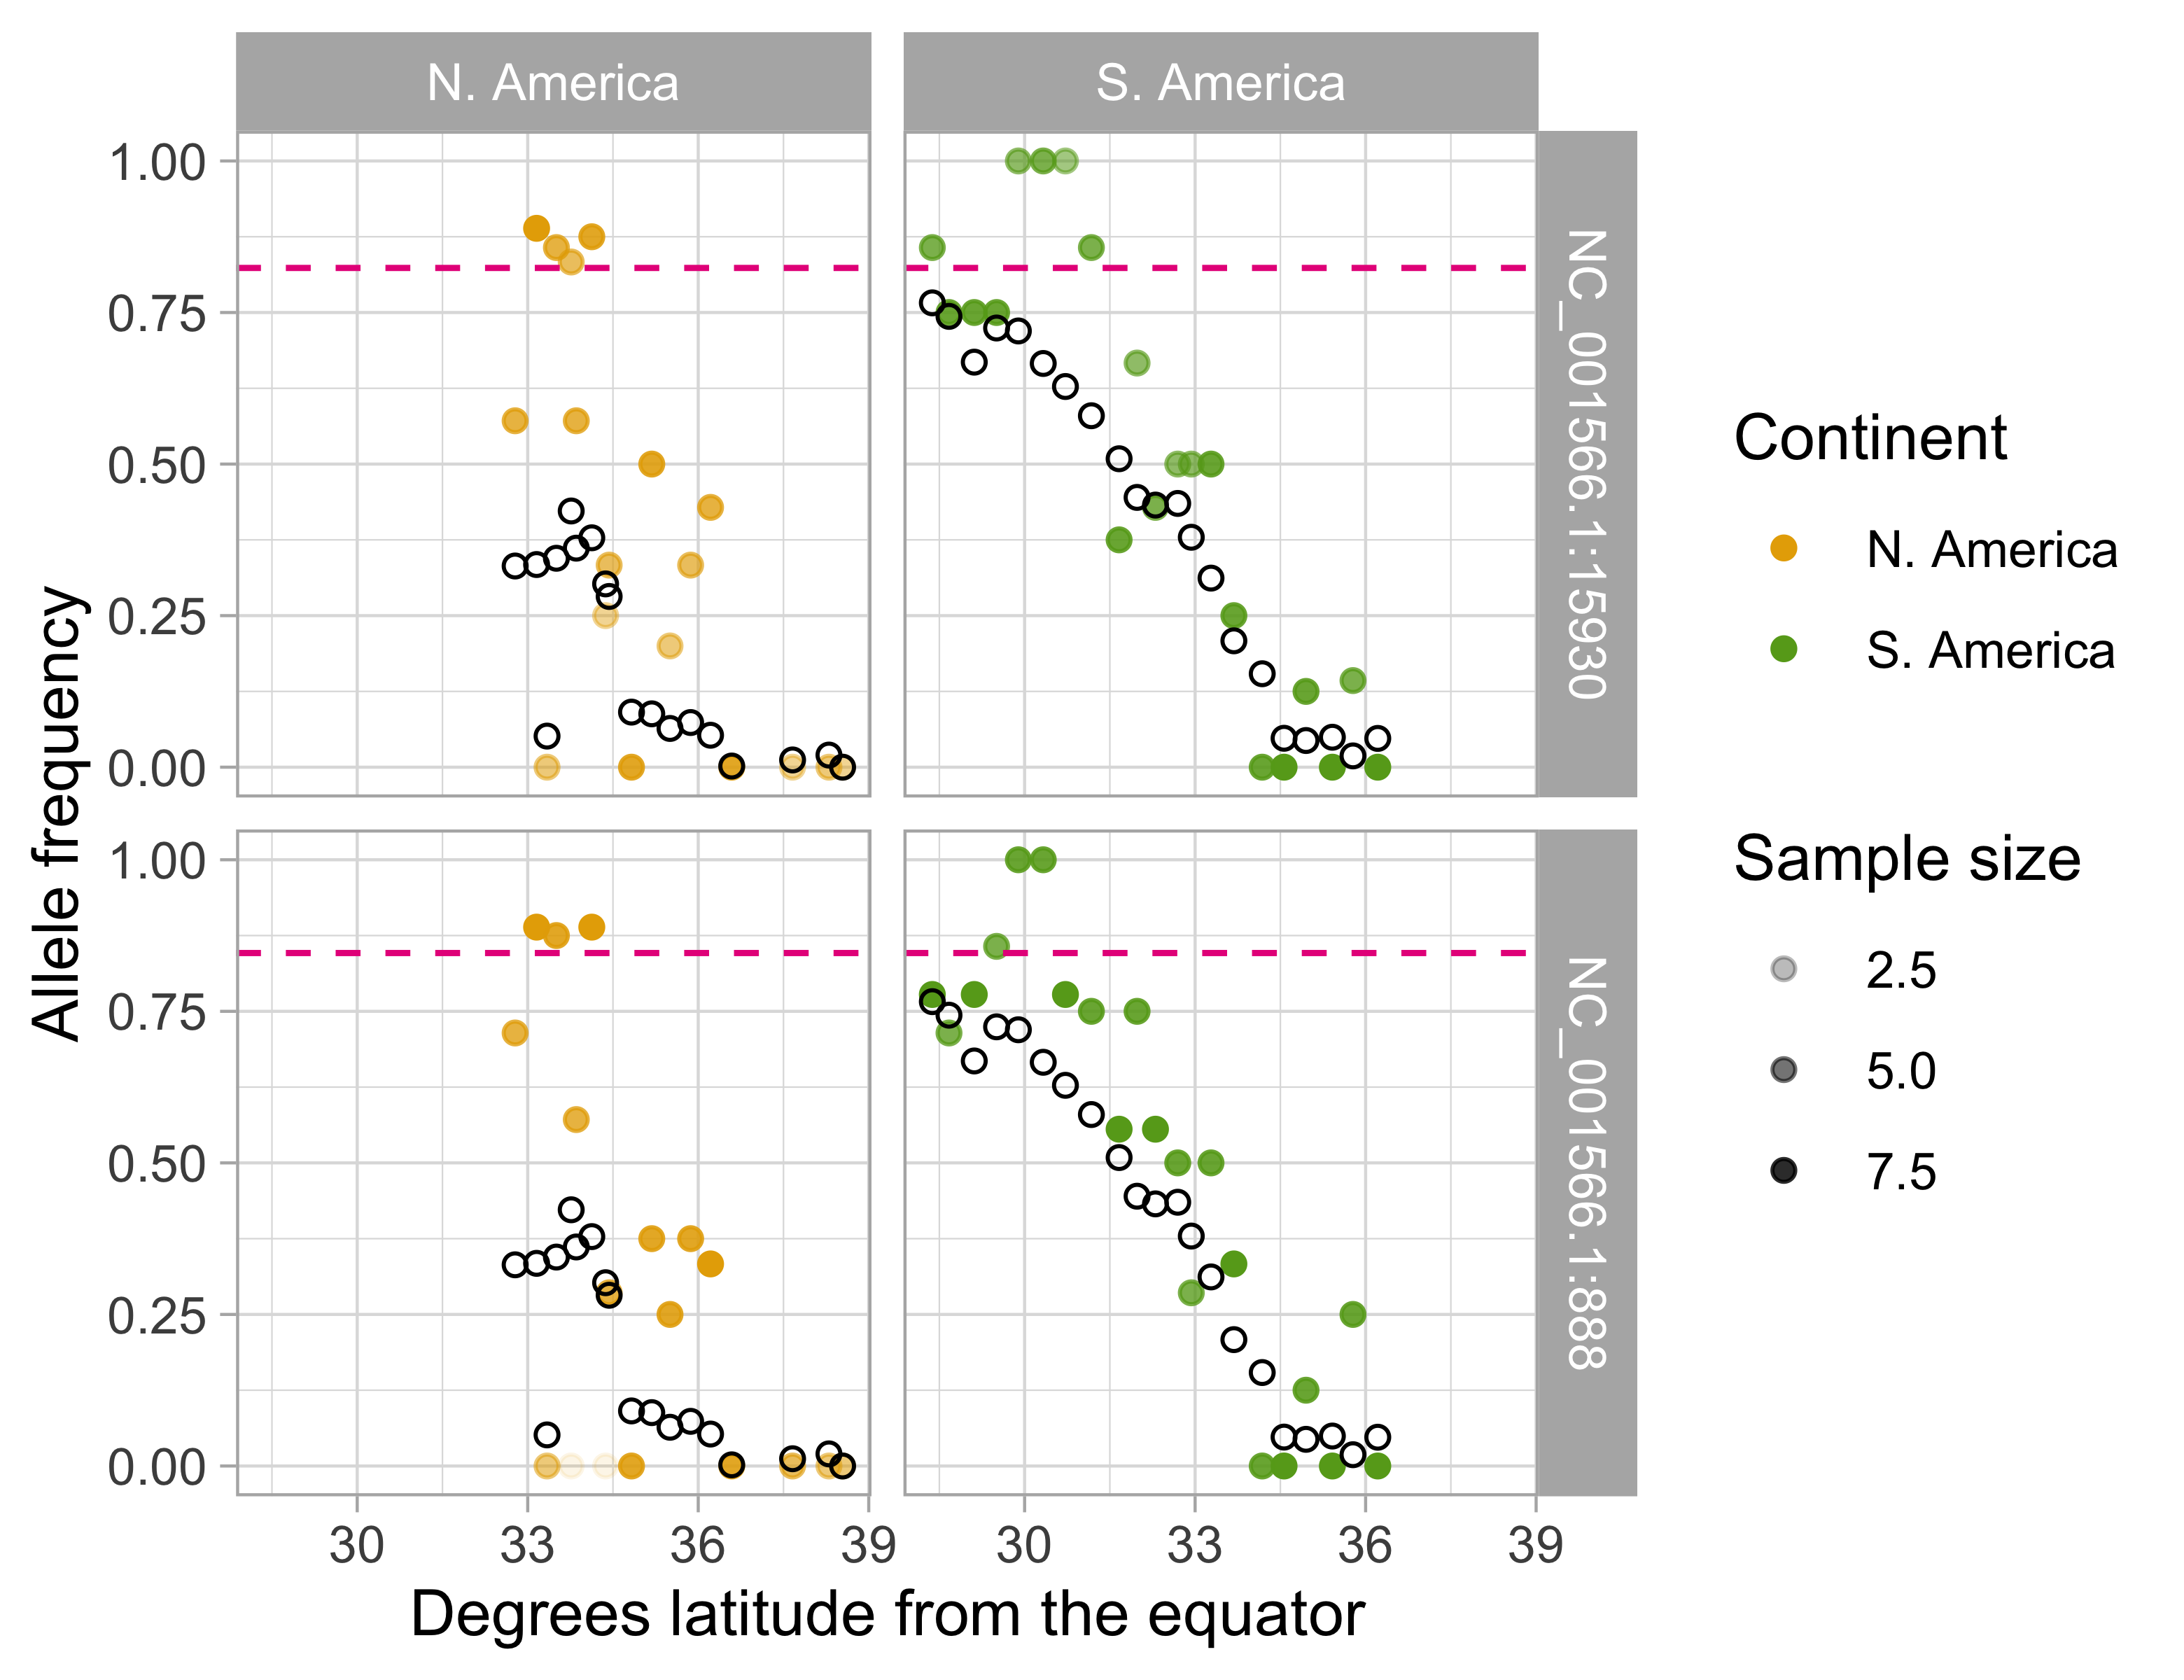
\includegraphics[width=\textwidth]{chapter1/figures/mtdna_snp_clines.png}
\caption{ \textbf{Mitochrondrial clines.} Out of 82 SNPs on the mitochrondria, we identified two with more than 80\% estimated frequency difference between \scutellata\ (A) and European (C \& M) reference panels. Estimated allele frequencies at these SNPs for each population in North America (left) and South America (right) are plotted in color. For comparison, population mean genomewide \A\ \anc\ proportions (NGSAdmix) are plotted as open black circles. At both SNPs, estimated M and C allele frequencies are zero (not shown) and estimated A allele frequencies are high but not at fixation (plotted as pink dashed lines). Bees sequenced in this study have low coverage across most of the mtDNA sequence, which prevented us from constructing a phylogenetic tree for full mitochondrial haplotypes and creates uncertainty in our allele frequency estimates here. To reflect this uncertainty, points are shaded by the sample size (i.e. the number of mtDNA haplotypes in a population for which we were able to call a consensus base).}
\label{mtdna_snps}
\end{figure}


   \chapter{Selective sorting of ancestral introgression in maize and teosinte along an elevational cline}
   
\begin{flushleft}

\begin{center}
Erin Calfee\textsuperscript{1,2},
Daniel Gates\textsuperscript{2,7},
Anne Lorant\textsuperscript{3,5},
M. Taylor Perkins\textsuperscript{2,6},
Graham Coop\textsuperscript{1,2,$\dagger$}, and
Jeffrey Ross-Ibarra\textsuperscript{1,2,4,$\dagger$}
\end{center}
\bigskip

\textsuperscript{1} Center for Population Biology, University of California, Davis, United States of America \\
\textsuperscript{2} Department of Evolution and Ecology, University of California, Davis, United States of America \\
\textsuperscript{3} Department of Plant Sciences, University of California, Davis, United States of America \\
\textsuperscript{4} Genome Center, University of California, Davis, United States of America \\
\textsuperscript{5} Laboratoire de Biologie Moléculaire et Cellulaire du Cancer, Hôpital Kirchberg, Luxembourg (current address) \\
\textsuperscript{6} Plant Molecular and Cellular Biology Program, University of Florida, Gainesville, United States of America (current address) \\
\textsuperscript{7} Checkerspot, Inc., Berkeley, California, United States of America (current address) \\
$\dagger$ co-mentors.

\bigskip
\end{flushleft}

% the * after section prevents numbering
\section*{Abstract}
While often deleterious, hybridization can also be a key source of genetic variation and pre-adapted haplotypes, enabling rapid evolution and niche expansion. 
Here we evaluate these opposing selection forces on introgressed ancestry between maize (\textit{Zea mays} ssp. \textit{mays}) and its wild teosinte relative, \ec{\mexicana (\textit{Zea mays} ssp. \mexicana)}.
Introgression from ecologically diverse teosinte may have facilitated maize's global range expansion, in particular to challenging high elevation regions ($>$ 1500 m).
We generated low-coverage genome sequencing data for 348 maize and \mexicana individuals to evaluate patterns of introgression in 14 sympatric population pairs, spanning the elevational range of \ec{\mexicana}, a teosinte endemic to the mountains of Mexico. 
While recent hybrids are commonly observed in sympatric populations and \mexicana demonstrates fine-scale local adaptation, we find that the majority of \mexicana ancestry tracts introgressed $>$1000 generations ago.

This \mexicana ancestry seems to have maintained much of its diversity and likely came from a common ancestral source, rather than contemporary sympatric populations, resulting in relatively low $F_{ST}$ between \mexicana ancestry tracts sampled from geographically distant maize populations. 

Introgressed \mexicana ancestry is reduced in lower-recombination rate quintiles of the genome and around domestication genes, consistent with pervasive selection against introgression.
However, we also find \mexicana ancestry increases across the sampled elevational gradient and that high introgression peaks are most commonly shared among high-elevation maize populations, consistent with introgression from \mexicana facilitating adaptation to the highland environment. 
In the other direction, we find patterns consistent with adaptive and clinal introgression of maize ancestry into sympatric \mexicana at many loci across the genome, suggesting that maize also contributes to adaptation in \mexicana, especially at the lower end of its elevational range.
In sympatric maize, in addition to high introgression regions we find many genomic regions where selection for local adaptation maintains steep gradients in introgressed \mexicana ancestry across elevation, including at least two inversions: the well-characterized \ec{14 Mb} \textit{Inv4m} \ec{on chromosome 4} and a new 3 Mb inversion \textit{Inv9f} surrounding the \textit{macrohairless1} locus on chromosome 9. 
\ec{Most outlier loci with high \mexicana introgression} show no signals of sweeps or local sourcing from sympatric populations and so likely represent ancestral introgression sorted by selection, resulting in correlated but distinct outcomes of introgression in different contemporary maize landrace populations.


\section*{Introduction}

Interbreeding between partially diverged species or subspecies can result in admixed individuals with low fitness, e.g. due to hybrid incompatibilities \cite{Powell:2020_dmi, Zuellig_Sweigart:2018_dmi,Presgraves_2010}. 
Consistent with the view that hybridization is often deleterious, a growing number of species show evidence of pervasive selection against introgressed ancestry \cite{Brandvain:2014cq, Aeschbacher:2017_mimulus, Kenney_Sweigart:2016_mimulus, Nelson:2021_mimulus, Martin:2019_butterflies, Edelman:2019_butterfly, Sankararaman:2014_neanderthals, Harris:2016fp, Juric:2016jj, Schumer:2018hc}. 
At the same time, introgression can be a source of novel genetic variation and efficiently introduce haplotypes carrying sets of locally adapted alleles, with the potential for rapid adaptation to new ecological challenges \cite{Pfennig:2016}. 
Indeed, admixture has been linked to adaptive species radiations and/or rapid niche expansions in a number of natural systems, including mosquitoes \cite{Fontaine:2015_mosquito}, \textit{Drosophila} \cite{Suvorov:2021_drosophila}, butterflies \cite{Edelman:2019_butterfly}, cichlids \cite{Martin:2015_cichlidradiation}, sunflowers \cite{Rieseberg:2003_sunflower}, wild tomatoes \cite{Pease:2016_tomato_radiation} and yeast \cite{Eberlein:2019_yeast, Tusso:2019_yeast}. 
In addition, introgression from wild relatives has facilitated the broad range expansions of multiple domesticated crops (reviewed in \cite{Purugganan:2019_review} and \cite{Janzen:2019}), and gene flow from crops back into their wild relatives has in some cases opened up novel ‘weedy' niches \cite{Ellstrand:2013_weeds_introgression}. 

Maize (\textit{Zea mays} ssp. \textit{mays}) is an ideal system to study selection on admixed ancestry and the effects on range expansion, as it has colonized nearly every human-inhabited ecosystem around the world \cite{Hake_Ross-Ibarra:2015} and interbreeds with a number of wild relatives genetically adapted to distinct ecologies \cite{Hufford:2012_teosinte_model_system,Mammadov:2018_teo}. 
In Mexico, highland maize represents an early major niche expansion that may have been facilitated by introgression. 
Approximately 9 thousand years ago, maize (\textit{Zea mays} ssp. \textit{mays}) was domesticated in the Balsas River Valley in Mexico from a lowland-adapted sub-species of teosinte (\textit{Zea mays} ssp. \parviglumis \cite{Piperno:2009_9kbalsas}), which grows readily at sea level and up to about 2000 meters \cite{Gonzalez:2018}. 
In contrast, \textit{Zea mays} ssp. \mexicana, which diverged from \parviglumis about 60 thousand years ago \cite{Ross-Ibarra:2009_60k}, is endemic to highland regions in Mexico ($\sim$1500-3000 meters in elevation) where it has adapted to a number of ecological challenges: a cooler, drier climate with higher UV intensity, different soil nutrient composition, and a shorter growing season necessitating earlier flowering times \cite{Fustier:2019, Fustier:2017, Aguirre-Liguori:2019, Rodriguez:2006_flowering, Piazena_1996:UV}.
%UV (doesn't show UV is higher, but shows highland maize handles UV better:  https://onlinelibrary.wiley.com/doi/full/10.1111/j.1365-3040.2005.01329.x )

Maize was introduced as a crop to the mountains of Mexico around 6.2 thousand years ago \cite{Piperno:2001_highlands}, and it is thought that gene flow from \mexicana assisted in adaptation to high elevation selection pressures. 
Highland maize and \mexicana share a number of putatively adaptive phenotypes \cite{Wilkes:1967, Wilkes:1977vc}, including earlier flowering times for the shorter growing season \cite{Rodriguez:2006_flowering}, purple anthocyanin-based pigmentation which shields DNA from UV damage \cite{Stapleton_Walbot:1994_anthocyanin_uv} and increases solar heat absorption \cite{Barthakur:1974_anthocyanin}, and macrohairs on the leaf and stem sheath, which are thought to increase herbivore defense \cite{Moya-Raygoza:2016} and/or heat maintenance in colder environments \cite{Lauter:2004}.
Earlier studies using 50K SNP-chip data for highland populations \cite{Hufford:2013_crop_wild} or genomewide data for a small number of individuals \cite{Wang:2017, Gonzalez-Segovia:2019}, have shown that highland maize landraces have experienced significant admixture from \mexicana, reaching high frequency at some loci, consistent with adaptive introgression. 


While some highland and locally-adapted alleles may be beneficial to maize, many introgressed \mexicana alleles, especially those affecting domestication traits, should be selected against by farmers growing maize landraces. In addition, maize alleles introgressed into \mexicana should be selected against because maize has accumulated genetic load from reduced population sizes during domestication \cite{Wang:2017} and because domestication traits generally reduce fitness in the wild \cite{Meyer_Purugganan:2013_crops, Stitzer_Ibarra:2018, Doebley:2004}, e.g. loss of disarticulation and effective seed dispersal \cite{Wilkes:1967}. 



In this study, we generate whole genome sequencing to investigate genomic signatures of admixture and selection in paired maize landrace and sympatric \textit{mexicana} populations, sampled from 14 locations across an elevational gradient in Mexico. This expanded sampling of sympatric maize and \mexicana populations across Mexico, combined with genomewide data and a well-parameterized null model, improves our ability to more formally test for adaptive introgression and identify likely source populations. The source of introgression is of interest, as teosinte demonstrates local adaptation to different niches within the highlands and there is significant genetic structure between \mexicana ecotypes \cite{Wilkes:1967, Fukunaga:2005fx, Pyhajarvi:2013jc, Fustier:2017, OBrien:2019}. Thus we can test whether local \mexicana populations are the ongoing source for geographically-restricted locally adaptive haplotypes.
We use this comprehensive genomic dataset to characterize the bi-directional timing and origin of introgression and evaluate the patterns and scale of natural selection for and against admixture between these taxa. 

\section*{Results and Discussion}

\subsection*{Genomewide \mexicana ancestry is structured by elevation}

We sampled paired sympatric populations from 14 geographically dispersed locations to assess the extent of gene flow between maize and \mexicana in Mexico.
Maize today is grown across the entire elevational range of its wild relatives, from sea-level up to 4000 meters \cite{Staller:2016}.
Our sampled sites range from 1547-2600 meters in elevation, which spans a large portion of \mexicana's range and exceeds the upper elevational range for maize's wild ancestor, \parviglumis (Fig \ref{map}).
For each of 14 maize/\mexicana sympatric sample locations, we resequenced 7-15 individuals per subspecies. We additionally sequenced 43 individuals from 3 \mexicana reference populations, totalling 348 low-coverage genomes (mean $\sim$1x). \ec{Two of these reference populations are documented to have no adjacent maize agriculture within the past 50 years, while a third higher elevation population (Amecameca) was chosen because it grows above the elevational range of \parviglumis, and thus outside of the historical range of maize. For simplicity, we refer to these three populations as an ‘allopatric' \mexicana reference panel, in contrast to our sympatric population pairs, but we note that maize has been grown extensively across Mexico and thus gene flow from maize into \mexicana is possible in recent generations at Amecameca, and historically at all three locations. We asses gene flow into these \mexicana reference populations below}.
For an allopatric maize reference population, we added 55 previously published high-coverage genomes from Palmar Chico \cite{Chen:2020_maize55}\ec{, which sits below the elevational range of \mexicana.}

\begin{figure}[ht]
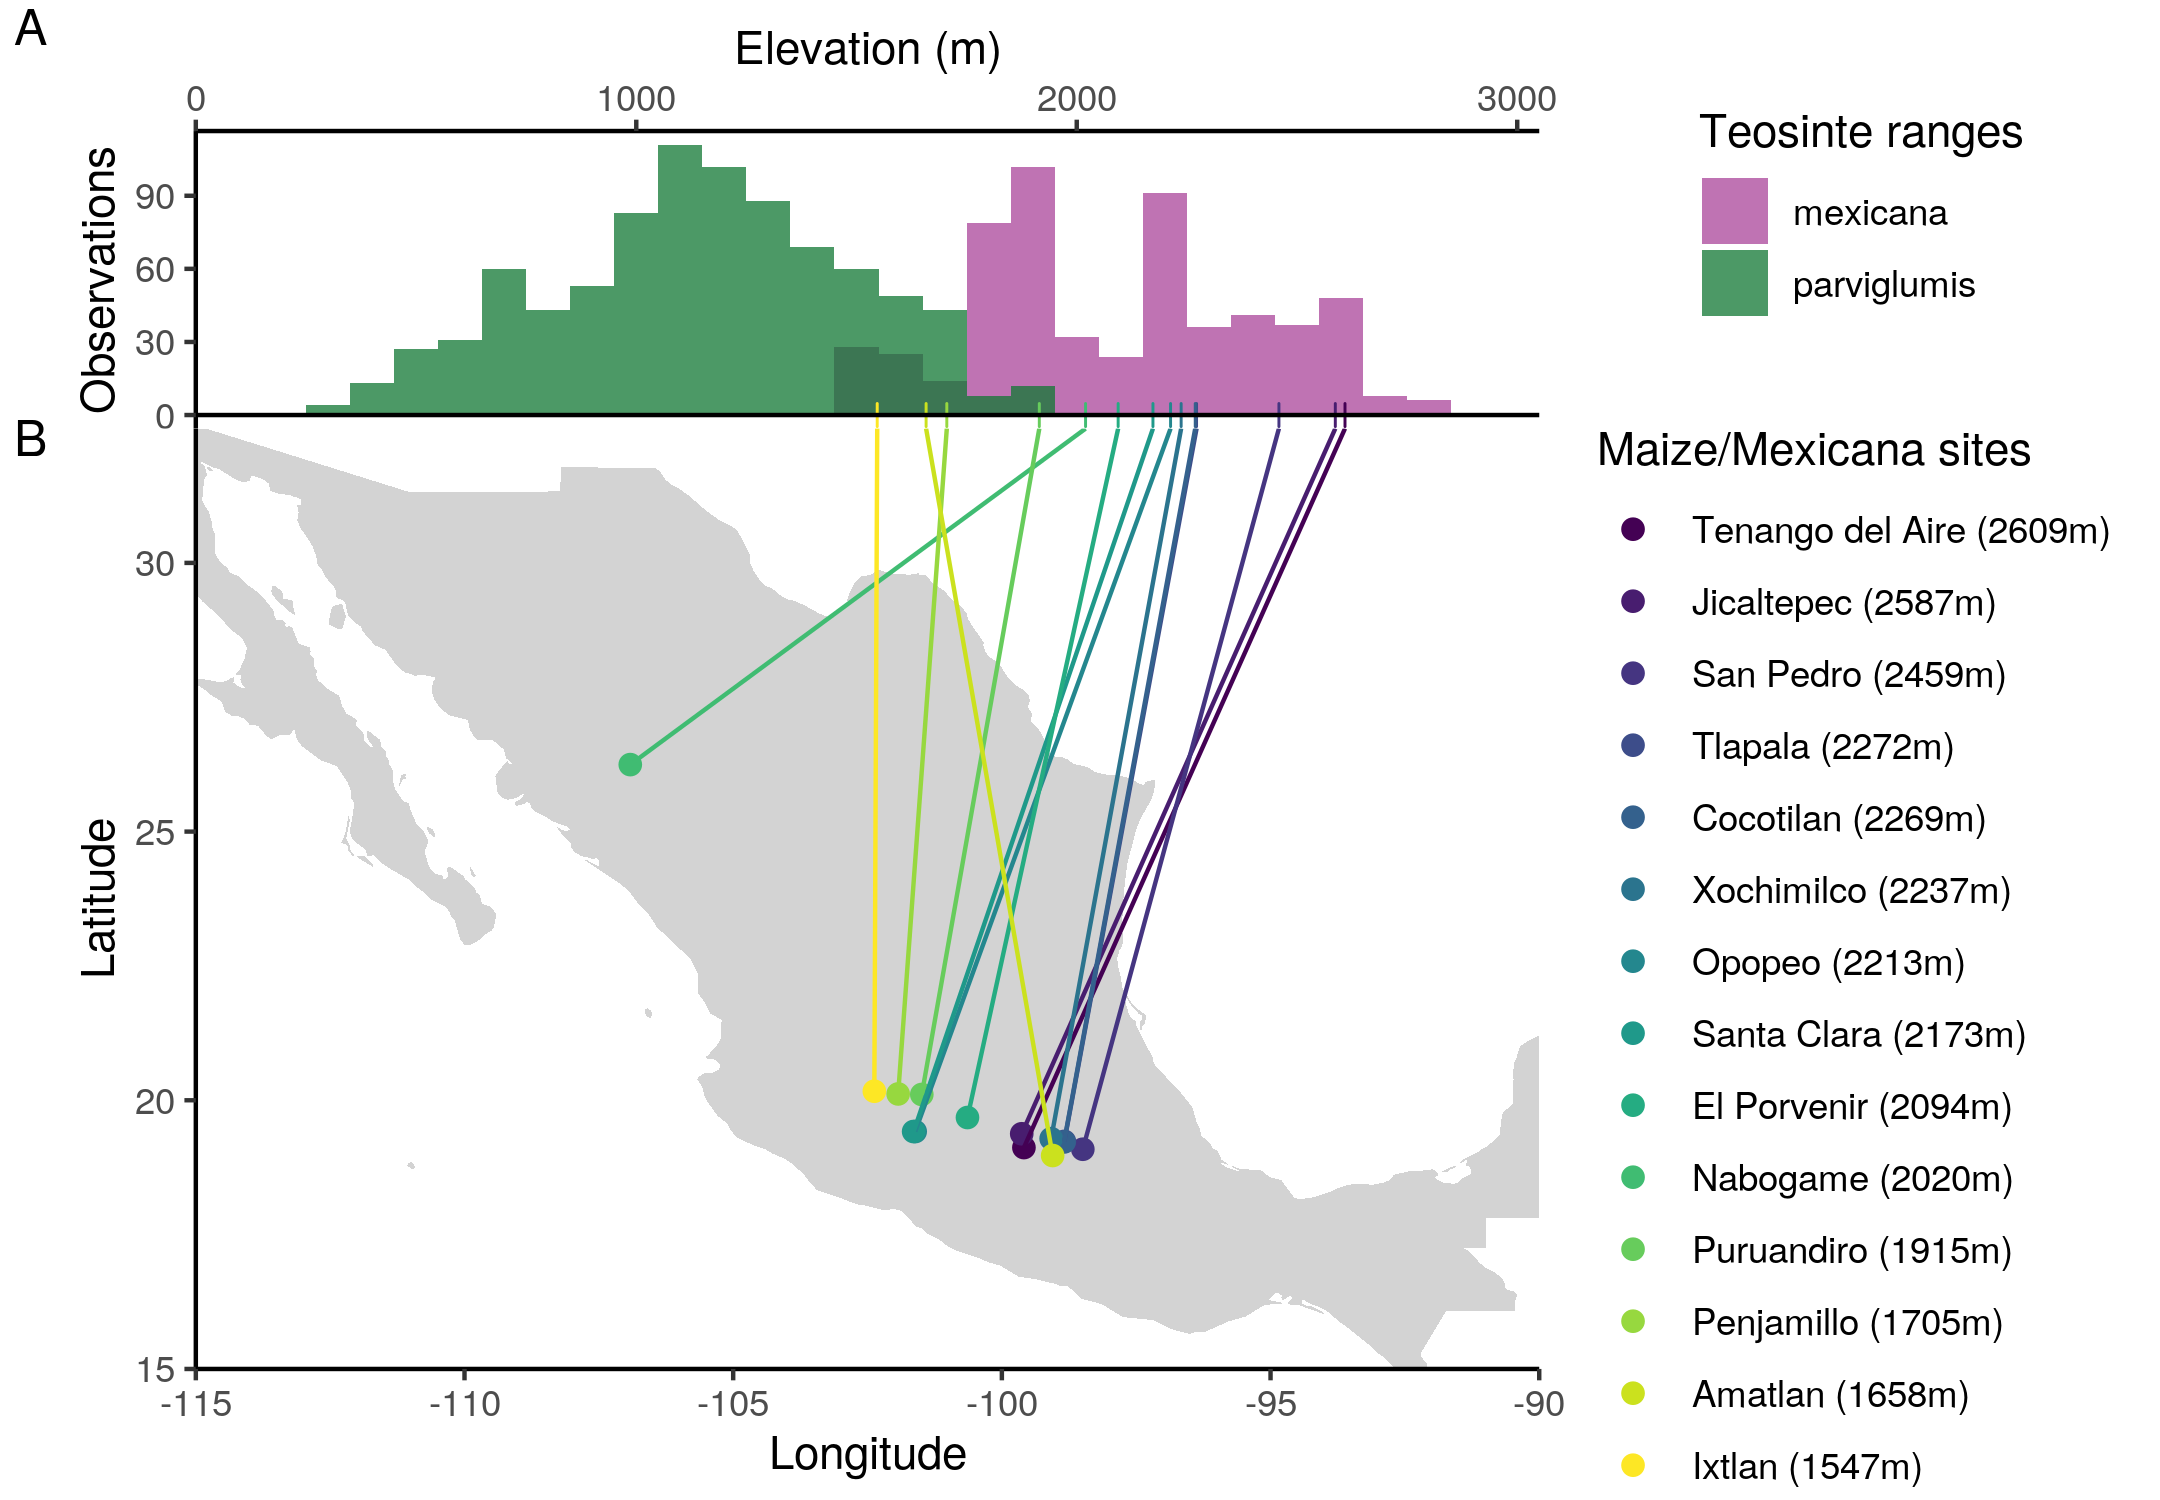
\includegraphics[width=\textwidth]{chapter2/figures/mexico_lines_elev_teo_color.png}
\caption{\color{Gray} \textbf{Sampled sympatric maize/\mexicana populations compared to distribution of teosintes} (A) Elevational range of teosintes based on historical occurrence data (1842-2016) from \cite{Gonzalez:2018}. (B) Geographic location and elevation of contemporary sympatric maize and \mexicana population pairs sampled across 14 sites in Mexico.}
\label{map}
\end{figure}

Principal components analysis of genetic diversity clearly separates maize and \mexicana, with putative admixed individuals from sympatric populations having intermediate values along PC1 (PCAngsd, Fig \ref{pca_maize_mex}). 

To estimate genomewide ancestry proportions for each individual, we ran NGSAdmix \cite{Skotte:2013_NGSadmix} with K=2 genetic clusters and genotype likelihoods for all maize and \mexicana individuals.
The two genetic clusters clearly map onto maize and \mexicana ancestry, with no indication of gene flow into the allopatric maize reference population but small amounts of maize ancestry in two of the three allopatric \mexicana populations (Fig \ref{global_anc_multi}A). 

Furthermore, we find a positive association between ancestry proportion and elevation (km), with higher \mexicana ancestry at higher elevations in both sympatric maize ($\beta=0.196, P = 1.42 \times 10^{-29}$) and sympatric \mexicana ($\beta=0.197, P = 4.38 \times 10^{-19}$) individuals (Fig \ref{global_anc_multi}B).

Increasing \mexicana ancestry at higher elevations is consistent with selection favoring \mexicana ancestry at higher elevations, but could also be due to purely demographic processes, e.g. a higher density of (wind-dispersed) \mexicana pollen at higher elevations, or increased gene flow from non-admixed maize populations at lower elevations. \ec{While most populations have admixture proportions well-predicted by their elevation, outlier populations may be the result of recent colonization histories for some locations or adaptation to other environmental niches. Within teosintes, elevation is a major axis of niche separation between \parviglumis (the ancestor of maize) and \mexicana \cite{Pyhajarvi:2013jc}, but genetic differentiation also correlates with soil nutrient content and at least four principal components constructed from climatic variables \cite{Aguirre-Liguori:2019}}.

%\begin{figure}[h!tb]
\begin{figure}[ht]
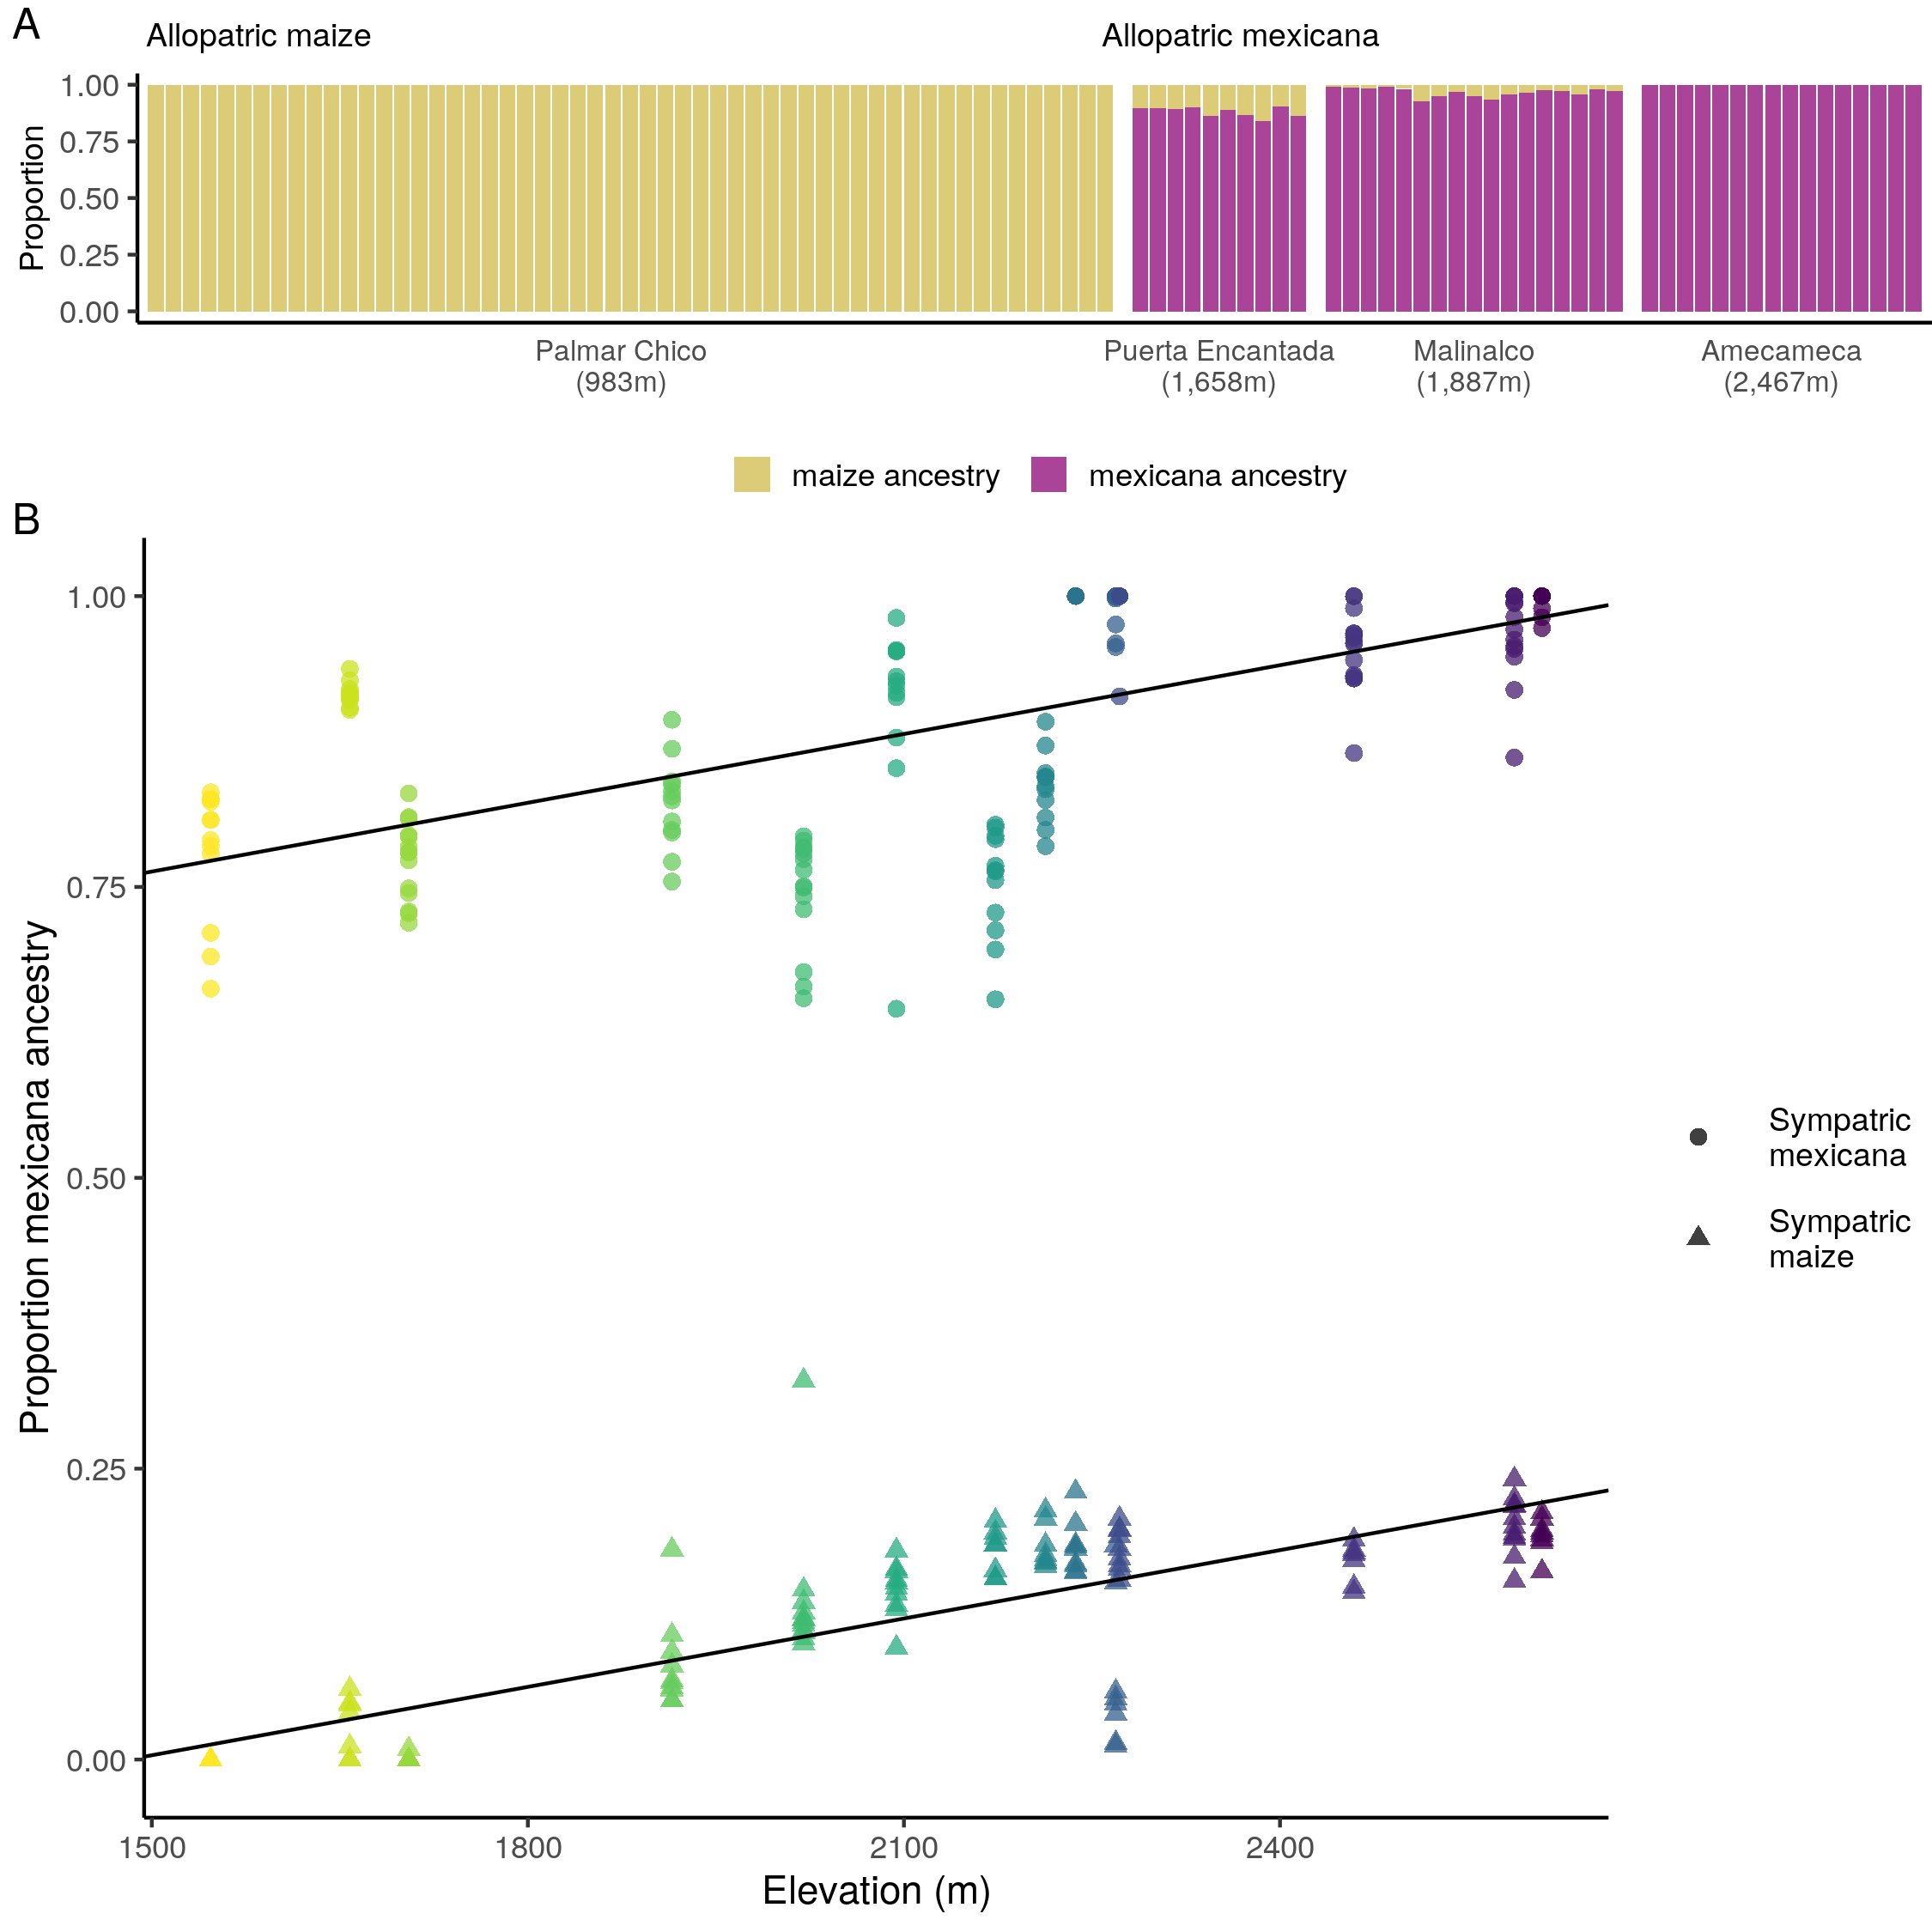
\includegraphics[width=\textwidth]{chapter2/figures/global_anc_multi.png}
\caption{\color{Gray} \textbf{Distribution of \mexicana ancestry by elevation} (A) Genomewide ancestry estimates (NGSAdmix) for allopatric maize and \mexicana reference individuals, grouped by sampling location. (B) Genomewide \mexicana ancestry estimates (NGSAdmix) for sympatric maize and \mexicana individuals (n = 305) along an elevational gradient, colored by sampling location. Lines show best linear model fit for \mexicana ancestry by elevation for each subspecies separately.}
\label{global_anc_multi}
\end{figure}

\subsection*{Origin and timing of introgression}
If \mexicana ancestry found in contemporary landrace genomes facilitated maize's colonization of the highlands approximately 6.2 thousands years ago \cite{Piperno:2001_highlands}, we would expect introgressed ancestry tracts to be short, due to many generations of recombination, and possibly to be derived from an ancient source population common to many present-day maize populations.
To test these predictions, we estimated local ancestry across the genome for individuals from each sympatric maize and \mexicana population using a hidden Markov model \ec{(HMM)} based on read counts (\cite{CorbettDetig:2017gh} see methods).
\ec{For each admixed population, this} \ec{HMM} simultaneously estimates local ancestry and, \ec{by optimizing the transition rate between different (hidden) ancestry states,} the generations since admixture.

Admixture is generally old, with median estimates of 1203 generations for sympatric maize populations and 718 generations for sympatric \mexicana populations (Fig \ref{time_admix}).

Because this HMM fits a single-pulse model to what was almost certainly multiple admixture events over time, we caution against over-interpretation of exact dates.
Multiple pulses or ongoing gene flow biases estimates towards the more recent pulse(s) \cite{Moorjani:2011_rolloff, Loh:2013_alder} and even old estimates do not exclude the possibility of limited more recent admixture.

These single-pulse approximations do, however, provide evidence that a large proportion of the introgression, especially into maize, is found on short ancestry tracts and therefore relatively old. 
%<<JEFF: is it worth text or supp. summary of ancestry tract lengths in cM? as a direct observation that is easy to intuit and supports this argument?>>

To identify likely source population(s) for introgressed ancestry, we compared $F_{ST}$ between all sympatric populations using only reads from high-confidence homozygous ancestry tracts (posterior $>$ 0.8) for maize and \mexicana ancestry separately.
We find that most \mexicana ancestry in maize resembles other \mexicana ancestry introgressed into other maize populations, rather that \mexicana ancestry from the local sympatric \mexicana population (Fig \ref{fst_within_ancestry}).
This finding is consistent with most introgressed ancestry being drawn from a communal source population, but none of the sympatric \mexicana populations have low enough $F_{ST}$ to tracts introgressed into maize to be a recent source.
While we cannot rule out recent introgression from an unsampled source population, the timing of our admixture estimates is more consistent with divergence of \mexicana ancestry, once introgressed into a maize background, from its original source population(s) (Fig \ref{time_admix}). Additionally, \mexicana ancestry tracts in maize have only slightly reduced genetic diversity ($\pi$, Fig \ref{pi_mexicana_ancestry_peaks}), meaning many \mexicana haplotypes have introgressed into maize at any given locus, with no evidence of a strong historical bottleneck.

\begin{figure}[ht]
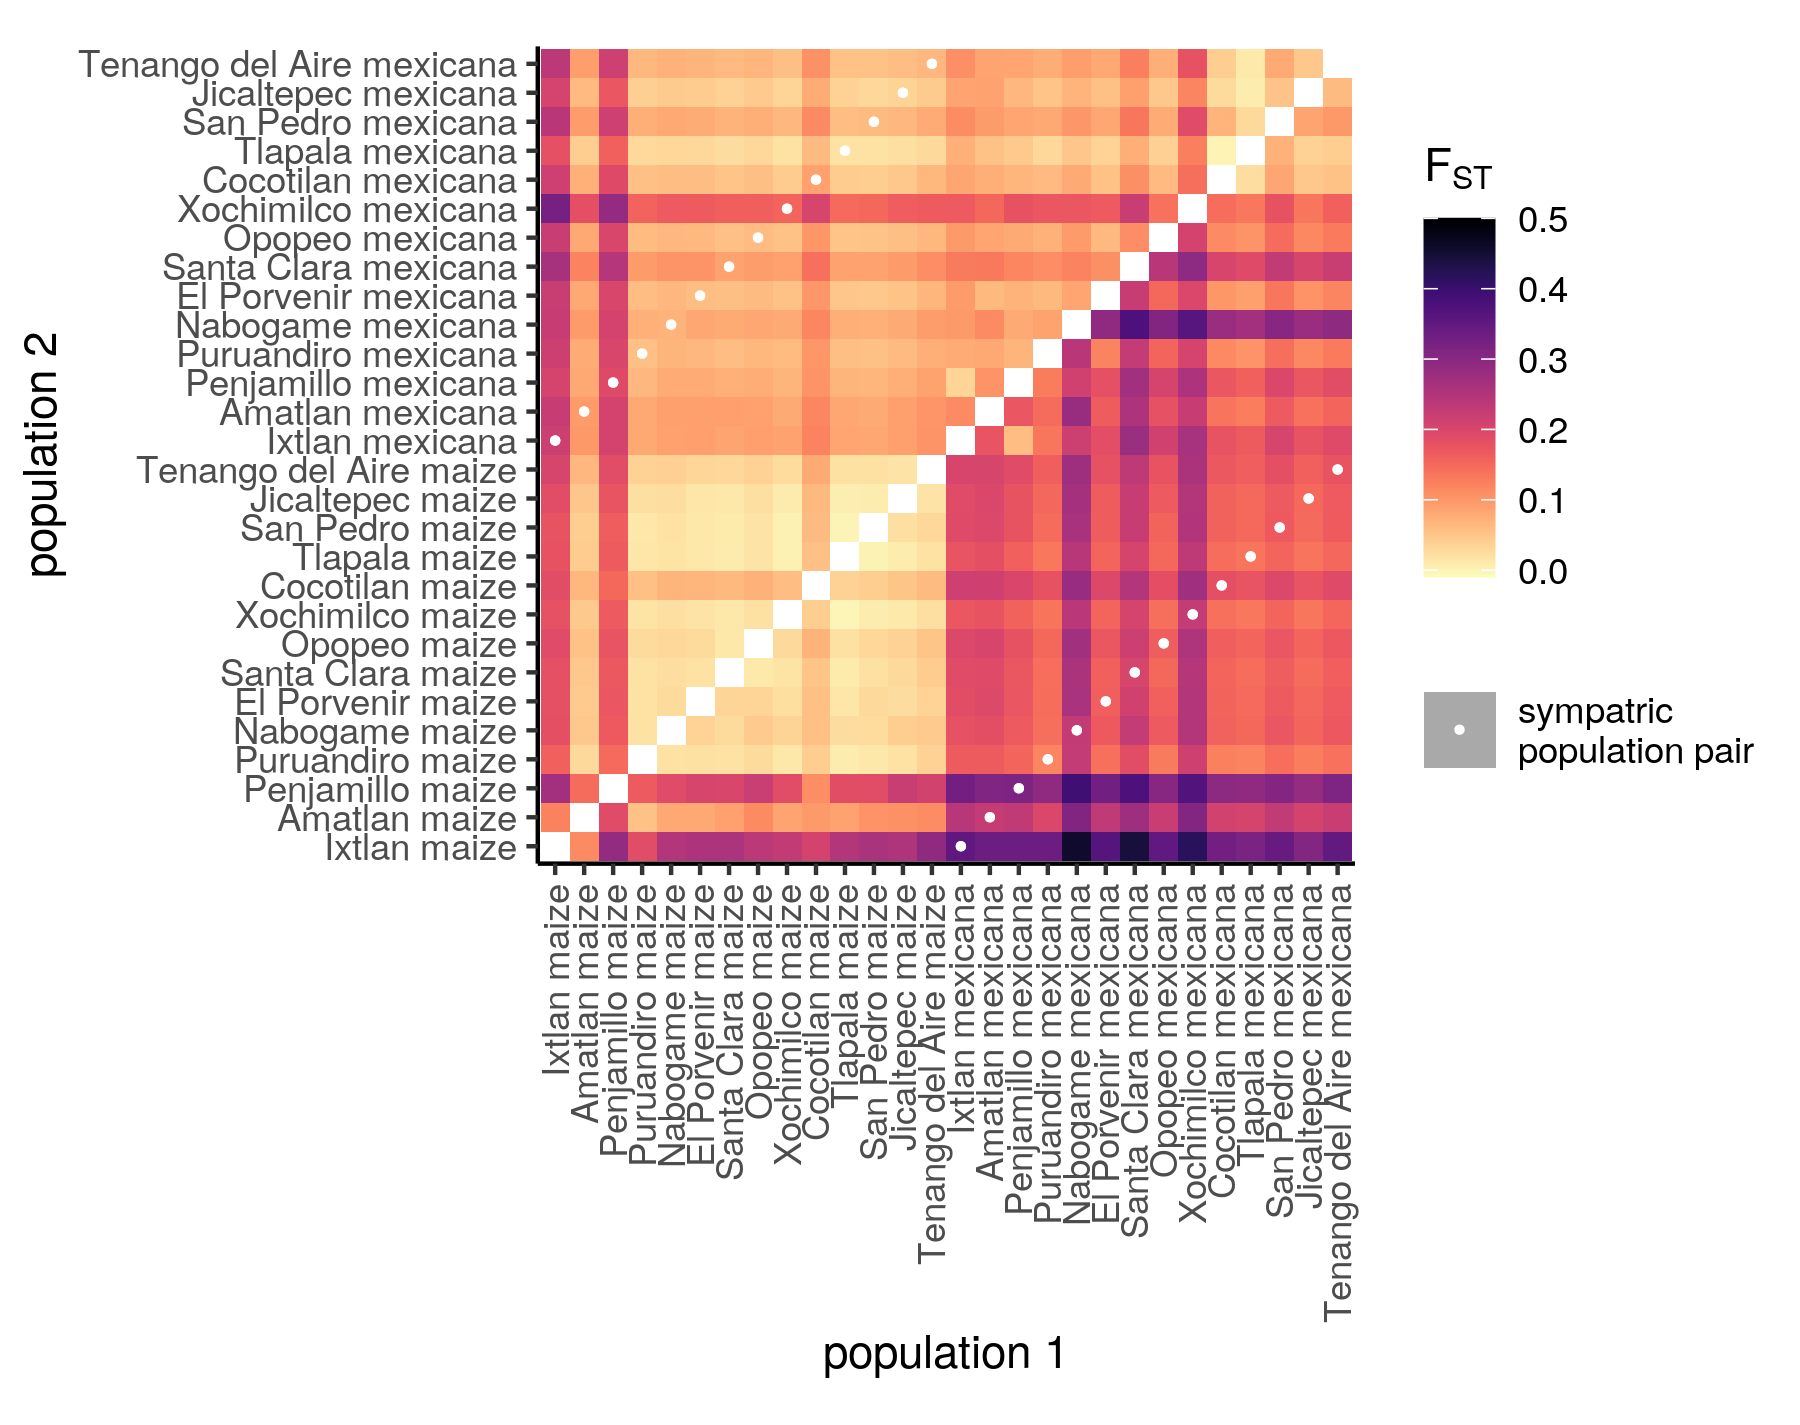
\includegraphics[width=\textwidth]{chapter2/figures/fst_within_maize_or_mexicana_ancestry_genomewide_heatmap_both.png}
\caption{\color{Gray} \textbf{$F_{ST}$ between ancestry tracts from different populations} 
Pairwise $F_{ST}$ between maize ancestry tracts from population 1 (x-axis) and population 2 (y-axis) are shown in the upper left triangle, while $F_{ST}$ estimates for \mexicana ancestry tracts are shown in the lower right triangle. 
Populations are sorted by subspecies, then elevation. Local sympatric maize-\mexicana population pairs are highlighted with a white dot \ec{and do not show reduced $F_{ST}$ relative to other (non-local) maize-\mexicana comparisons. 
Additionally, introgressed \mexicana ancestry shows low differentiation between maize populations (creating a light-colored maize block in the lower right triangle) and no potential \mexicana source populations show especially low $F_{ST}$ with this block.
%In addition, the light-colored maize corner in the lower right triangle shows that introgressed \mexicana ancestry has low differentiation between maize populations, consistent with shared drift post-admixture, but no potential \mexicana source populations show especially low $F_{ST}$ with this corner. 
Light coloring generally across the upper left triangle reflects the low differentiation within maize, providing little information to distinguish between potential maize ancestry sources.}}
\label{fst_within_ancestry}
\end{figure}

Two lower elevation maize populations are an exception to this general pattern: Ixtlan and Penjamillo. These populations have higher $F_{ST}$ between their introgressed ancestry tracts and other \mexicana tracts in maize \ec{(Fig \ref{fst_within_ancestry})}, more recent timing of admixture estimates \ec{(Fig \ref{time_admix})}, and reduced genetic diversity (Figs \ref{pi_mexicana_ancestry_peaks}-\ref{pi_maize_ancestry}).
These patterns could be caused by small population sizes and more recent independent admixture, although $F_{ST}$ does not identify a likely \mexicana source population.
Consistent with this interpretation, we have evidence that local maize at Ixtlan is at least partially descended from recently introduced commercial seed (relayed by local farmers \cite{Hufford:2013_crop_wild}). 

The lack of a clear reduction in $F_{ST}$ for \mexicana ancestry tracts between sympatric population pairs, combined with older timing of admixture estimates, indicates that while contemporary hybridization may occur in the field between maize crops and adjacent  \mexicana populations, this is not the source for the bulk of the introgressed ancestry segregating in highland maize. 

Instead, we propose that the majority of \mexicana ancestry in maize derives from admixture over 1000 years ago, possibly from a diverse set of \mexicana source populations over a large geographic and temporal span, and the resulting ancestry tracts are now distributed across different contemporary maize populations.
These genomewide average $F_{ST}$ results, however, do not exclude the possibility that particular regions were introgressed from one or more distinct, possibly local, source populations.

While we also analyzed $F_{ST}$ within high-confidence maize ancestry tracts, we found that maize ancestry is too homogeneous to make inferences about potential admixture source populations of maize into \mexicana (Figs \ref{fst_within_ancestry}, \ref{pi_maize_ancestry}). 

\subsection*{Selection against introgression genomewide} 
When there is widespread selection against introgressing variants at many loci across the genome, selection will more efficiently remove linked ancestry in regions of the genome with lower recombination rates, which creates a positive relationship between local recombination rate and the proportion of introgressed ancestry \cite{Veller:2019ge, Schumer:2018hc, Harris:2016fp, Juric:2016jj, Sankararaman:2014_neanderthals, Brandvain:2014cq, Aeschbacher:2017_mimulus, Kenney_Sweigart:2016_mimulus, Nelson:2021_mimulus, Martin:2019_butterflies, Edelman:2019_butterfly}.
To test whether such negative selection is shaping patterns of introgression genomewide in sympatric maize and \mexicana, we first divided the genome into quintiles based on the local recombination rates for 1 cM windows. 
We then ran NGSAdmix on the SNPs within each quintile separately, using K=2 clusters, to estimate maize and \mexicana ancestry proportions. We used a recombination map from maize \cite{Ogut:2015df}, which is likely to be correlated with other \textit{Zea} subspecies at least at the level of genomic quintiles, but a limitation of this analysis is that we do not have a recombination map for hybrid populations which means that e.g. segregating structural inversions will not necessarily show low recombination rates.

Our results from sympatric maize landraces are consistent with selection against \textit{mexicana} introgression at many loci genomewide, resulting in lower introgressed ancestry in regions of the genome with lower recombination rates (Fig \ref{K2_by_r}A). 
We find a positive Spearman's rank correlation between recombination rate quintile and mean introgressed \mexicana ancestry proportion ($\rho = 1,\ \text{CI}_{95}[0.85,\ 1.00]$), \ec{reflecting the fact that introgression increases monotonically across quintiles.}  \ec{A} similar analysis using $f_4$ statistics replicates this result (see methods, Fig \ref{f4_tree}-\ref{f4_maize_by_cd} and \nameref{spearmans_rho_f4_sympatric_maize_pop22}). The higher elevation maize populations show this pattern most starkly; while all individuals have low \mexicana ancestry for the lowest recombination rate quintile, some high elevation populations have individuals with over 40\% introgressed ancestry for the highest recombination rate quintile (Fig \ref{K2_by_r}B). Using a linear-model fit, we found a significant interaction between recombination rate quintile and the slope of ancestry across elevation in sympatric maize (\nameref{tbl_elev_r_interaction_5}). 
This is again consistent with low-recombination rate regions having a stronger effect of linked selection reducing \mexicana ancestry, with higher elevation maize landraces either experiencing larger amounts of gene flow or retaining more ancestry due to adaptive processes in high recombination regions (Fig \ref{K2_by_r_elev_lm}).


\begin{figure}[ht]
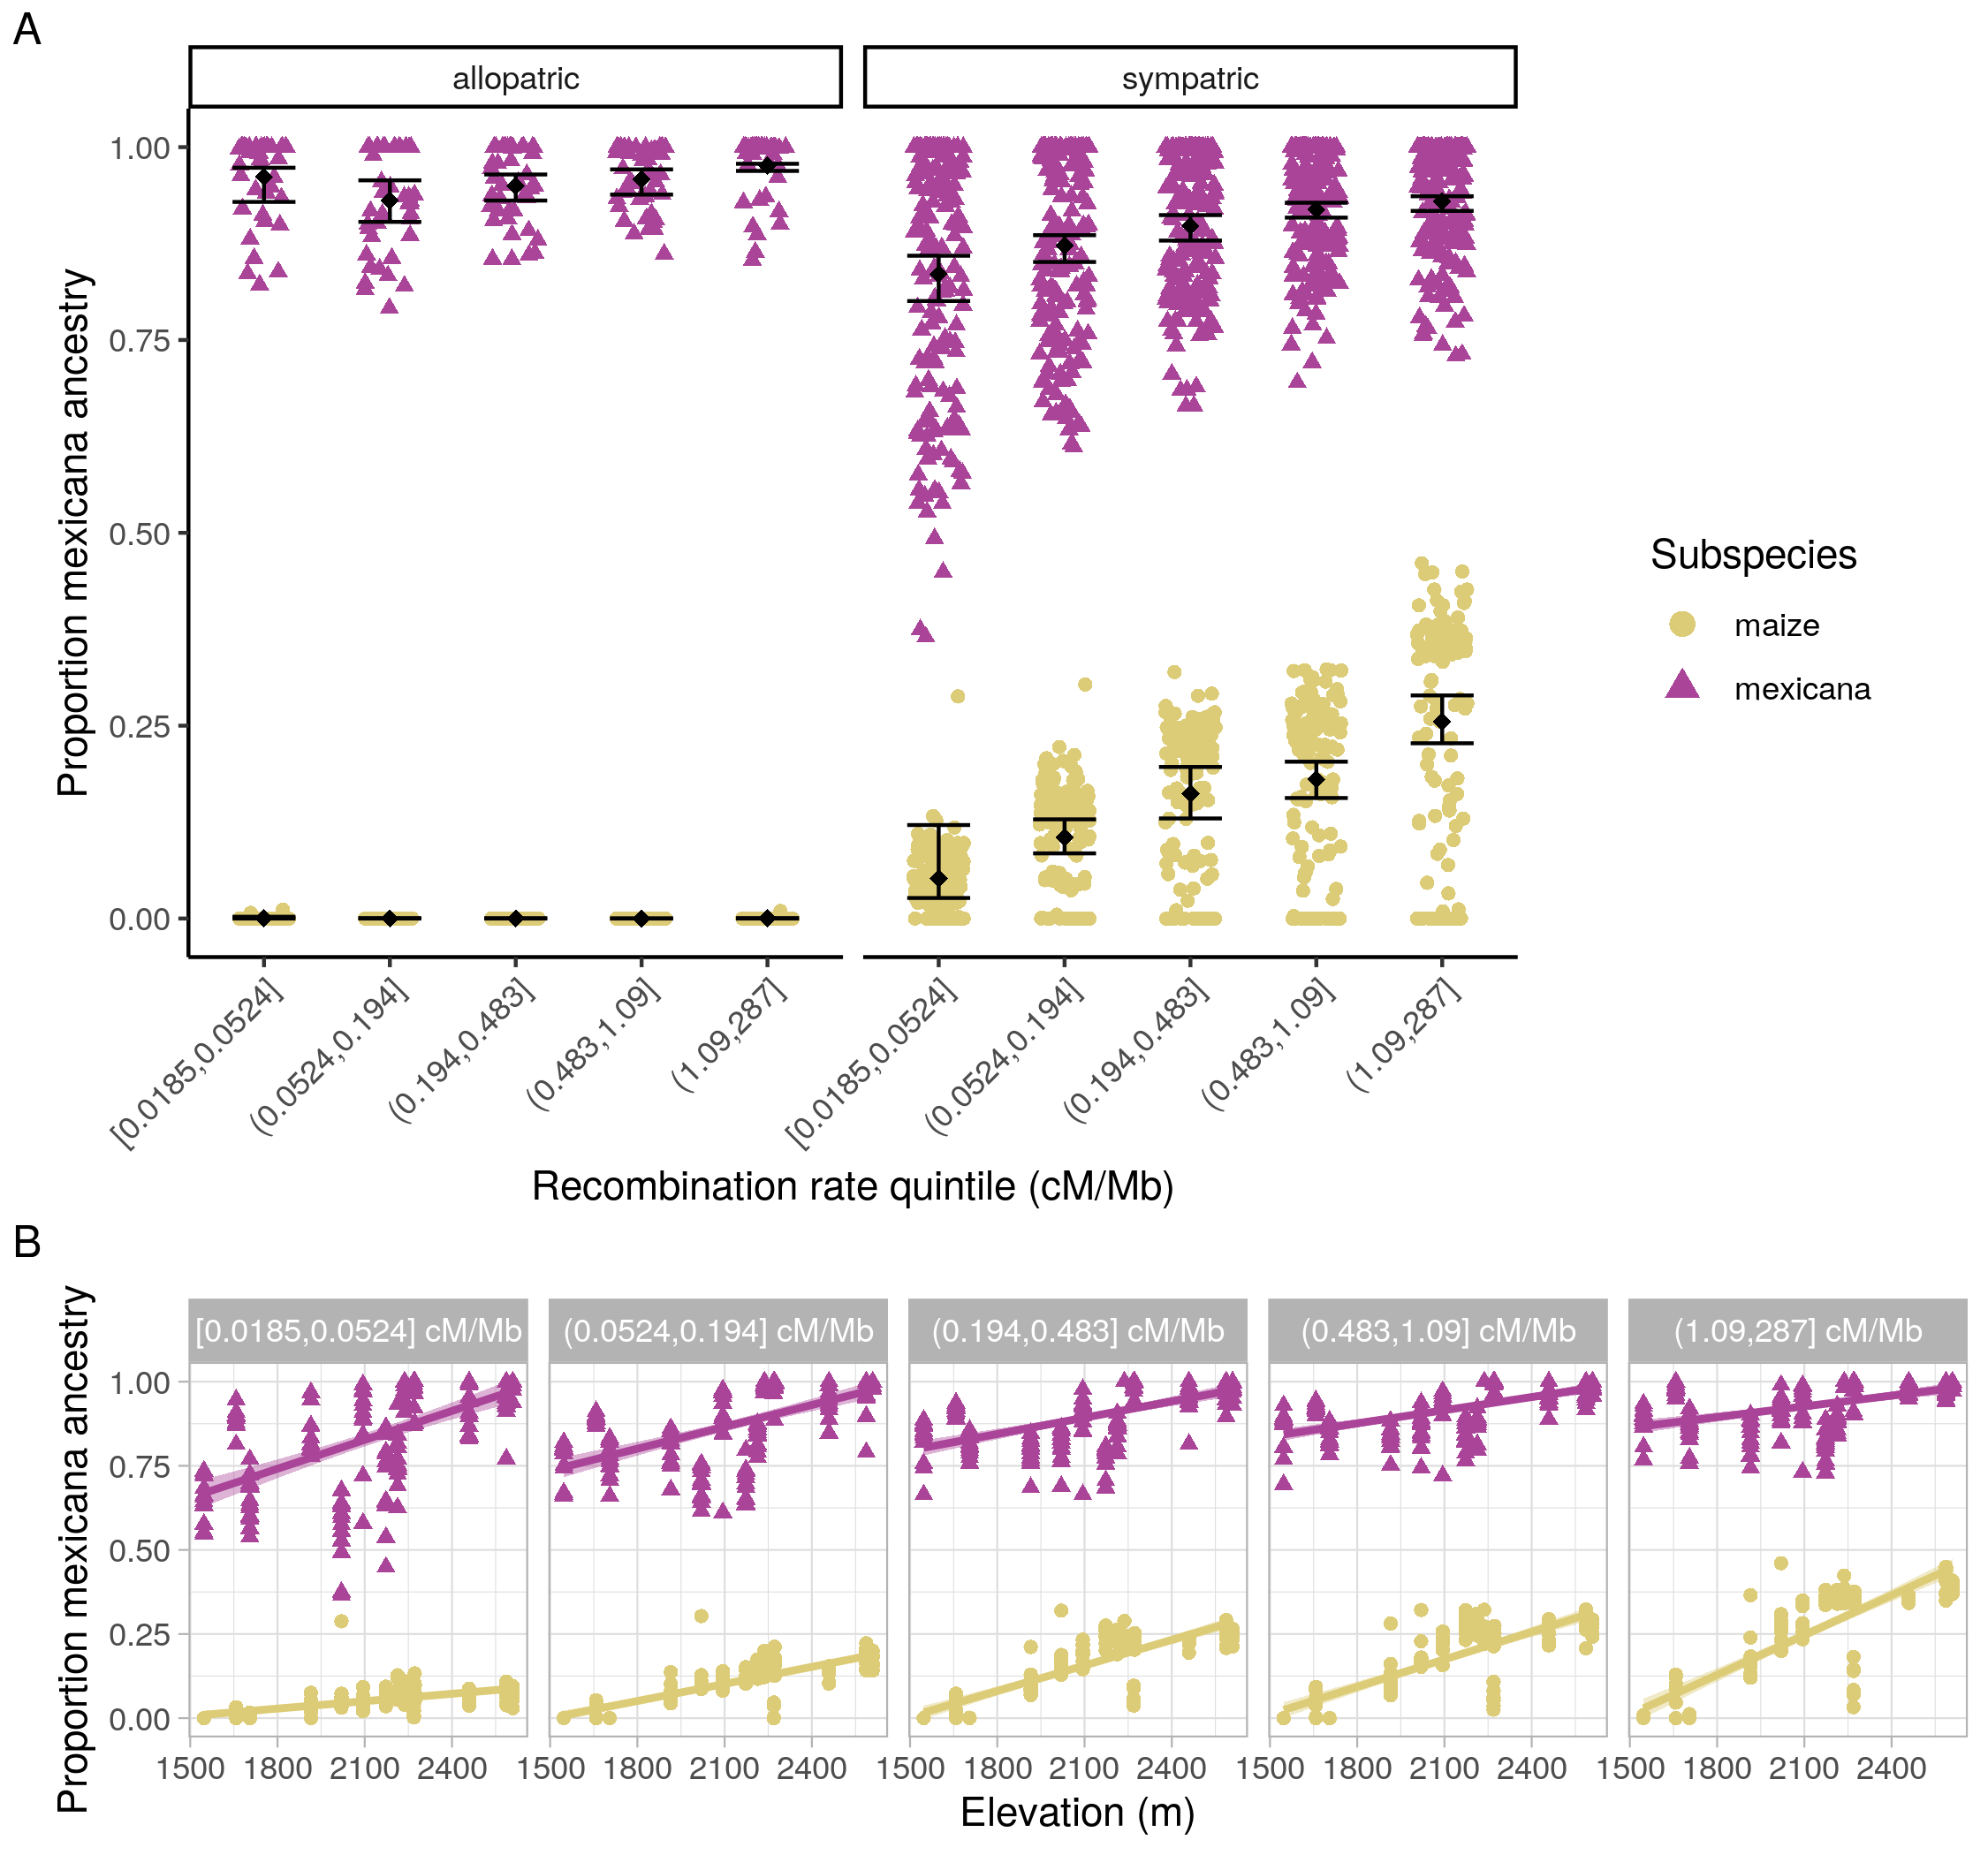
\includegraphics[width=.95\textwidth]{chapter2/figures/K2_by_r_multi_panel.png}
\caption{\color{Gray} \textbf{(A) \textit{Mexicana} ancestry by recombination rate}. Inferred \mexicana ancestry in  allopatric reference populations (left) and sympatric maize and \mexicana populations (right) using NGSAdmix (K=2) by recombination rate quintiles. Group mean and 95\% confidence interval based on bootstrap percentiles (n = 100) are depicted in black. Ancestry estimates for each individual are shown as points, colored by subspecies, and points are jittered for better visualization. (B) Slopes of \mexicana ancestry across elevation for each recombination rate quintile, based on NGSAdmix estimates. Each point is a sympatric maize or \mexicana individual and lines show the best-fit linear model for ancestry by elevation (with shaded 95\% confidence interval) estimated separately for each quintile and subspecies.}
\label{K2_by_r}
\end{figure} 

Because recombination rate is positively correlated with gene density in \textit{Zea} \cite{Schnable:2009_B73}, we also tested the Spearman's rank correlation between quintiles defined by coding base pairs per cM and their proportion introgressed \mexicana ancestry. 
Again we found evidence supporting pervasive selection against introgression (Fig \ref{K2_by_cd}, $\rho = -1,\ \text{CI}_{95}[-1,\ -0.85]$).

In contrast, sympatric \mexicana shows an unexpected negative relationship between recombination rate and introgression from maize, with more \mexicana ancestry (lower introgression) in the highest recombination rate regions of the genome ($\rho = 1,\ \text{CI}_{95}[0.9,\ 1]$). Correlations with coding bp per cM and based on $f_4$ statistics corroborate this pattern (see \ref{K2_by_cd}-\ref{f4_mexicana_by_cd} and \nameref{spearmans_rho_f4_sympatric_mexicana_pop22}). 
While one possible explanation is that introgressing maize ancestry is overall beneficial, not deleterious, a similar pattern could also be produced from a number of different distributions of fitness effects for maize alleles, including for example if most maize alleles are deleterious but some have strong beneficial consequences.
While maize ancestry in general is not predicted to provide adaptive benefits in teosinte, invasive \mexicana in Europe shows selective sweeps for maize ancestry at multiple loci that have contributed to its establishment as a noxious weed \cite{Le_Corre:2020} and we speculate that maize could be a source of alleles adapted to human-modified landscapes.

We repeated these analyses using local ancestry calls as our introgression estimates and found a non-significant Spearman's rank correlation between \mexicana ancestry and recombination rates for 1 cM windows in sympatric maize (Fig \ref{local_ancestry_mexicana_by_log10r}, $\rho = 0.011,\ \text{CI}_{95}[-0.039,\ 0.062]$) and a negative rank correlation between \mexicana ancestry and recombination rate in sympatric \mexicana ($\rho = -0.473,\ \text{CI}_{95}[-0.512,\ -0.432]$).
Contrasting results between global and local ancestry methods could be a reflection of true evolutionary differences across different time periods; local ancestry methods capture patterns from more recent gene flow that comes in longer ancestry blocks while STRUCTURE-like algorithms (NGSAdmix) and $f_4$ statistics are based on allele frequencies that collapse information across ancestry blocks of any size, capturing a longer evolutionary time scale.
This interpretation would suggest that \mexicana has experienced stronger selection against more recent maize gene flow than historical gene flow. 
%\jri{<<JEFF:we can test this? maybe come back to to test formally?} 
However, we caution that local ancestry methods may also have subtle biases in power that are sensitive to local recombination rates and make them less reliable for comparing ancestry patterns across recombination rate quintiles.

Overall, we find support for widespread selection against introgression into maize and mixed results from similar tests of this hypothesis in \mexicana.

\subsection*{High introgression peaks shared across populations}

To assess adaptive introgression in our sympatric populations, we identified introgression ‘peaks' where minor ancestry exceeds the genomewide mean by more than 2 standard deviations. We find no strong reduction in average diversity ($\pi$) for \mexicana ancestry at high introgression peaks (Fig \ref{pi_mexicana_ancestry_peaks}). 
This maintenance of diversity implies that selection at most peaks has favored multiple \mexicana haplotypes, and hard sweeps for a recent beneficial mutations on a specific haplotype are rare.

We observe that many high \textit{mexicana} ancestry peaks are shared across subsets of our 14 maize landrace populations (see e.g. chr4, Fig \ref{maize_chr4}). 
While most outlier peaks are unique to a single population, many peaks are shared across 7 or more of the populations (Fig \ref{combmatrix_peaks_maize}).
To a lesser extent, we also observe sharing of high-introgression peaks for maize ancestry in sympatric \mexicana populations (Fig \ref{combmatrix_peaks_mexicana}).

\begin{figure}[ht]
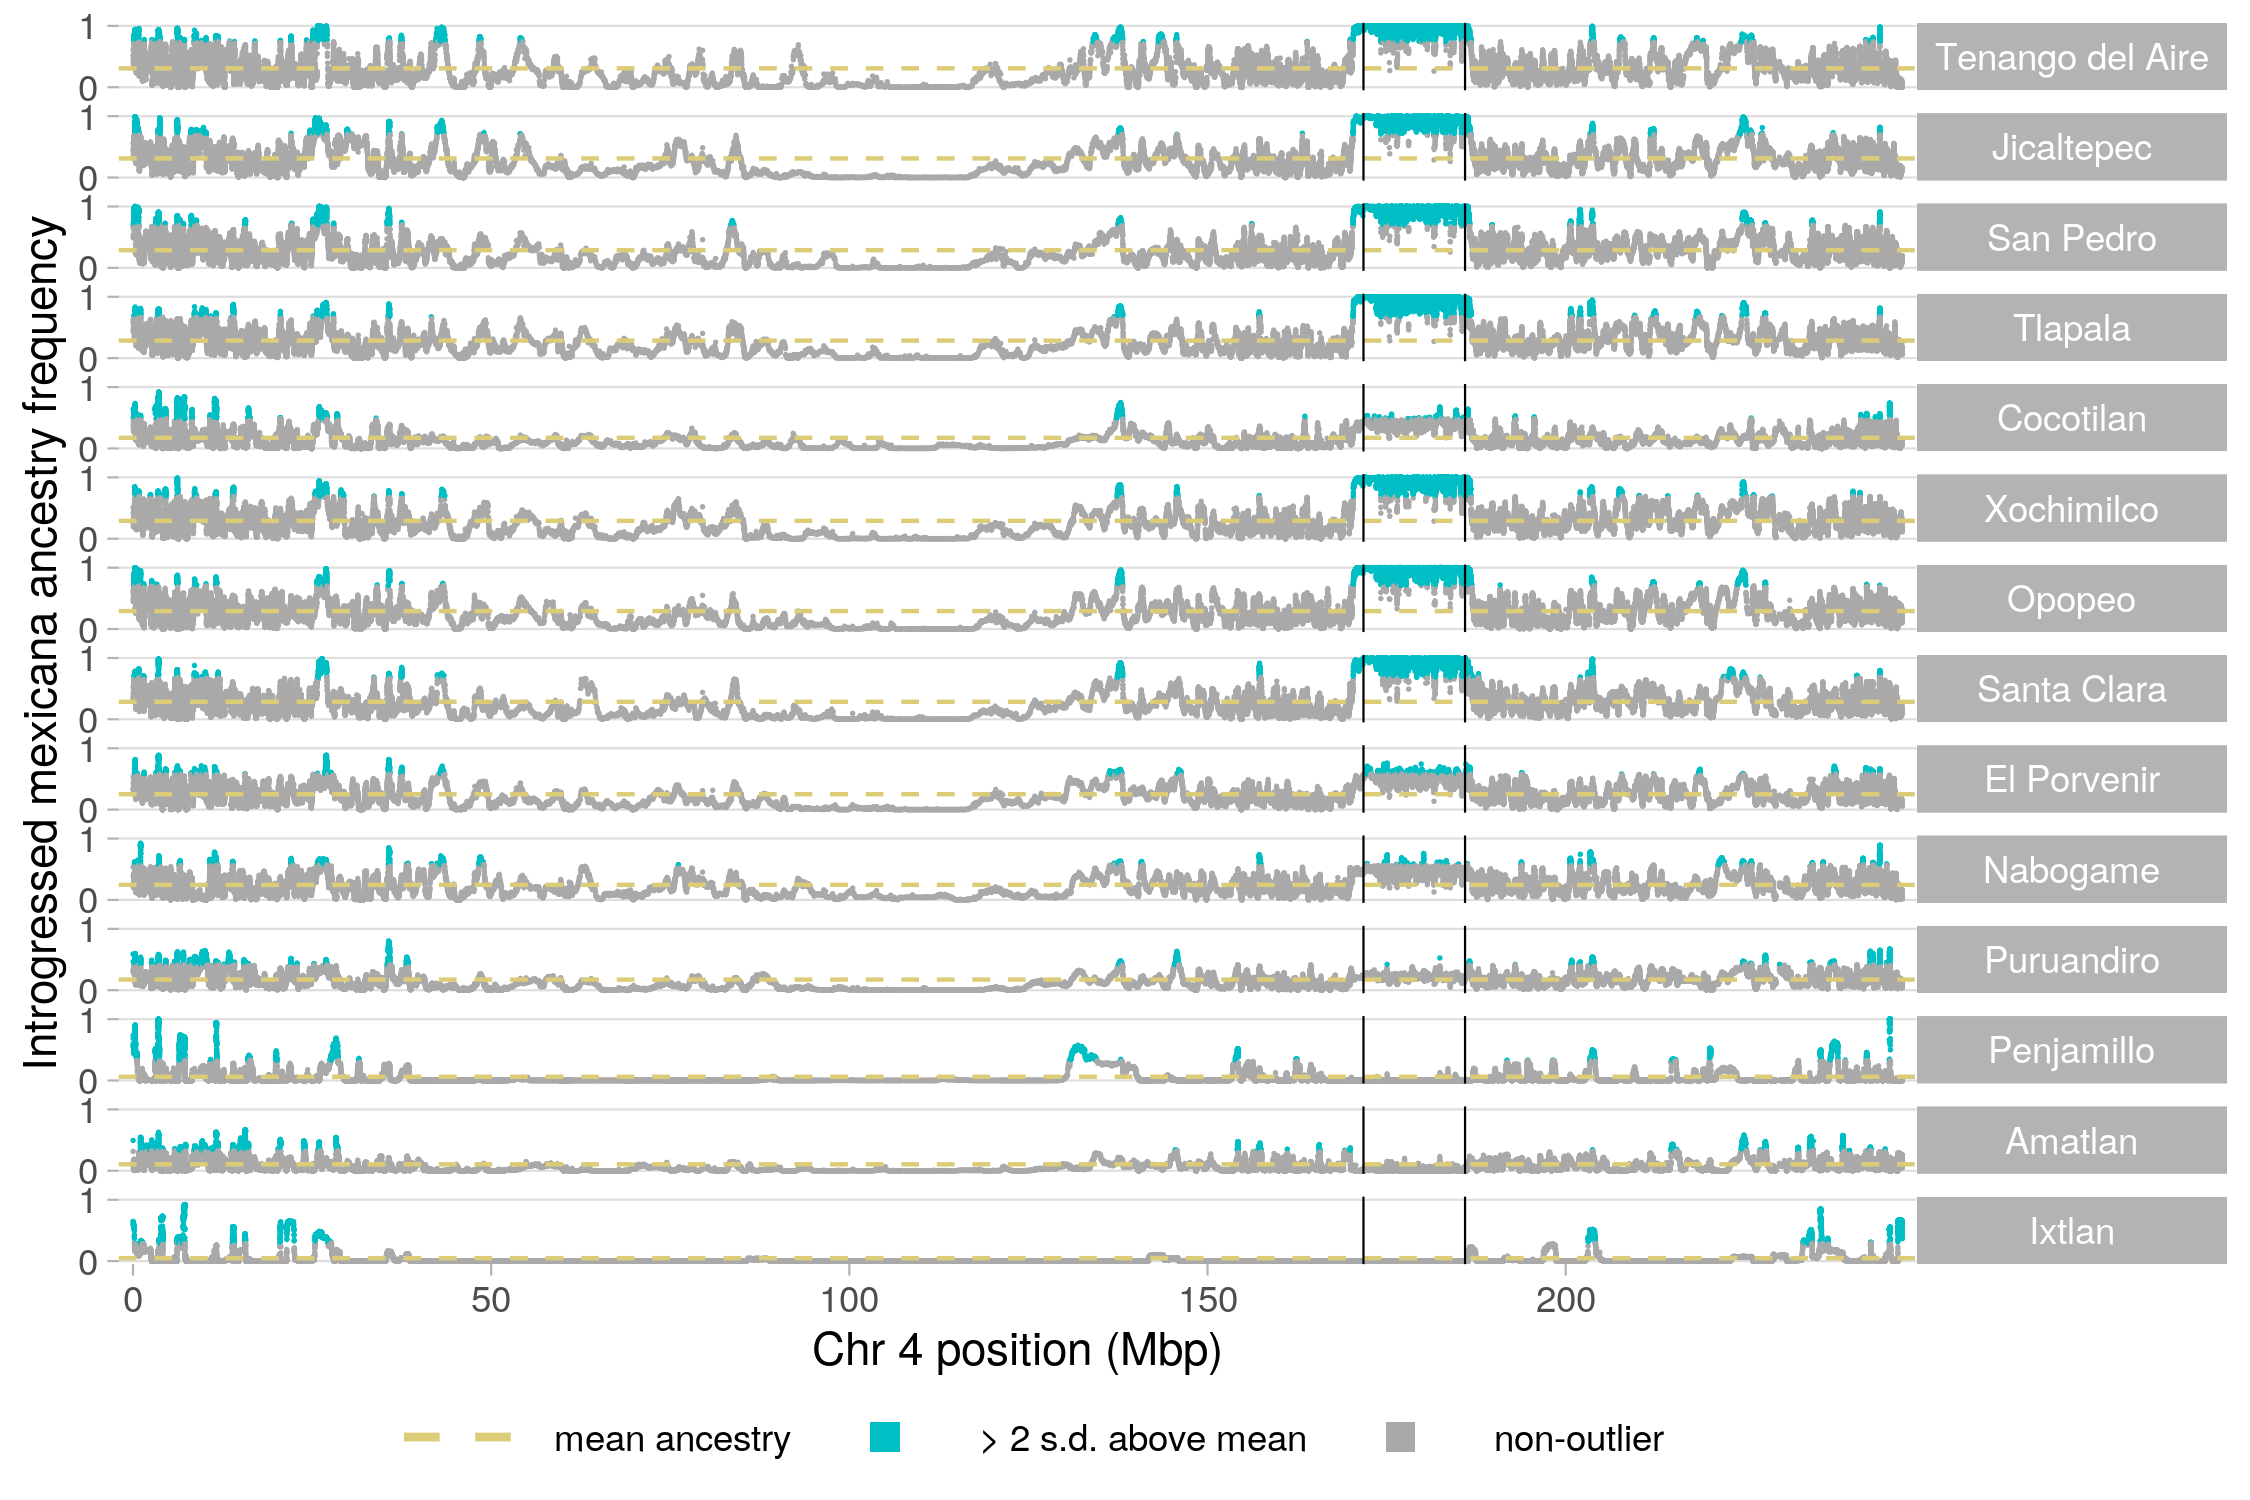
\includegraphics[width=.95\textwidth]{chapter2/figures/maize_shared_outliers_chr_4.png}
\caption{\color{Gray} \textbf{Introgression in maize landrace populations across chromosome 4}. Local introgressed ancestry frequency for each maize landrace population compared to their genomewide mean. Populations are ordered from high to low elevation (top to bottom). High introgression peaks with more than 2 standard deviations above the population mean introgressed \mexicana ancestry are highlighted in blue. Vertical black lines show the previously identified endpoints for a large inversion (\textit{Inv4m} coordinates from Fig 3 of \cite{Pyhajarvi:2013jc}). For local ancestry on other chromosomes \ec{and for sympatric \mexicana}, see Figs \ref{maize_chr1}-\ref{mexicana_chr10}}. 
\label{maize_chr4}
\end{figure}
% Turelli wants low to high elevation on side of plot
High introgression peaks in many independent populations would be very unexpected by chance. However, our sampled populations do not provide independent evidence for adaptive introgression, due to shared gene flow and drift post-admixture (e.g. long-distance human-assisted dispersal of maize seed). To estimate the rate of peak sharing we should expect from demographic processes alone, we simulated 100,000 unlinked loci under a multivariate normal distribution parameterized with the empirical ancestry variance-covariance matrix K (see methods). 
These simulations preserve the ancestry variance across loci within populations and non-independence in ancestry between populations.

For both sympatric maize and \mexicana, every population shares an excess of high introgression peaks with all other populations compared to expectations set by our MVN null model. 
However, peak sharing is most elevated among high elevation maize populations (with the exception of Cocotilan, see Fig \ref{network_peaks}). 
To investigate the origins of population-specific peaks of introgression, we calculated $F_{ST}$ between homozygous \mexicana ancestry in local maize and in each \mexicana population for these genomic regions.
Patterns of $F_{ST}$ between local sympatric pairs at local introgression peaks differed little from background $F_{ST}$ (Fig \ref{local_fst_peaks}), offering little support for the idea that population-specific peaks arose from recent, locally sourced, adaptive introgression.
Instead, patterns in maize are consistent with introgressed \mexicana ancestry tracts from old shared admixture being favored by natural selection, and thus rising to high frequency, in a subset of landraces. 
% I changed this wording because it wasn't accurate with the figure! We didn't compare local vs. non-local fst at peaks. Instead we compared local fst at peaks vs. non-peaks.

\begin{figure}[ht]
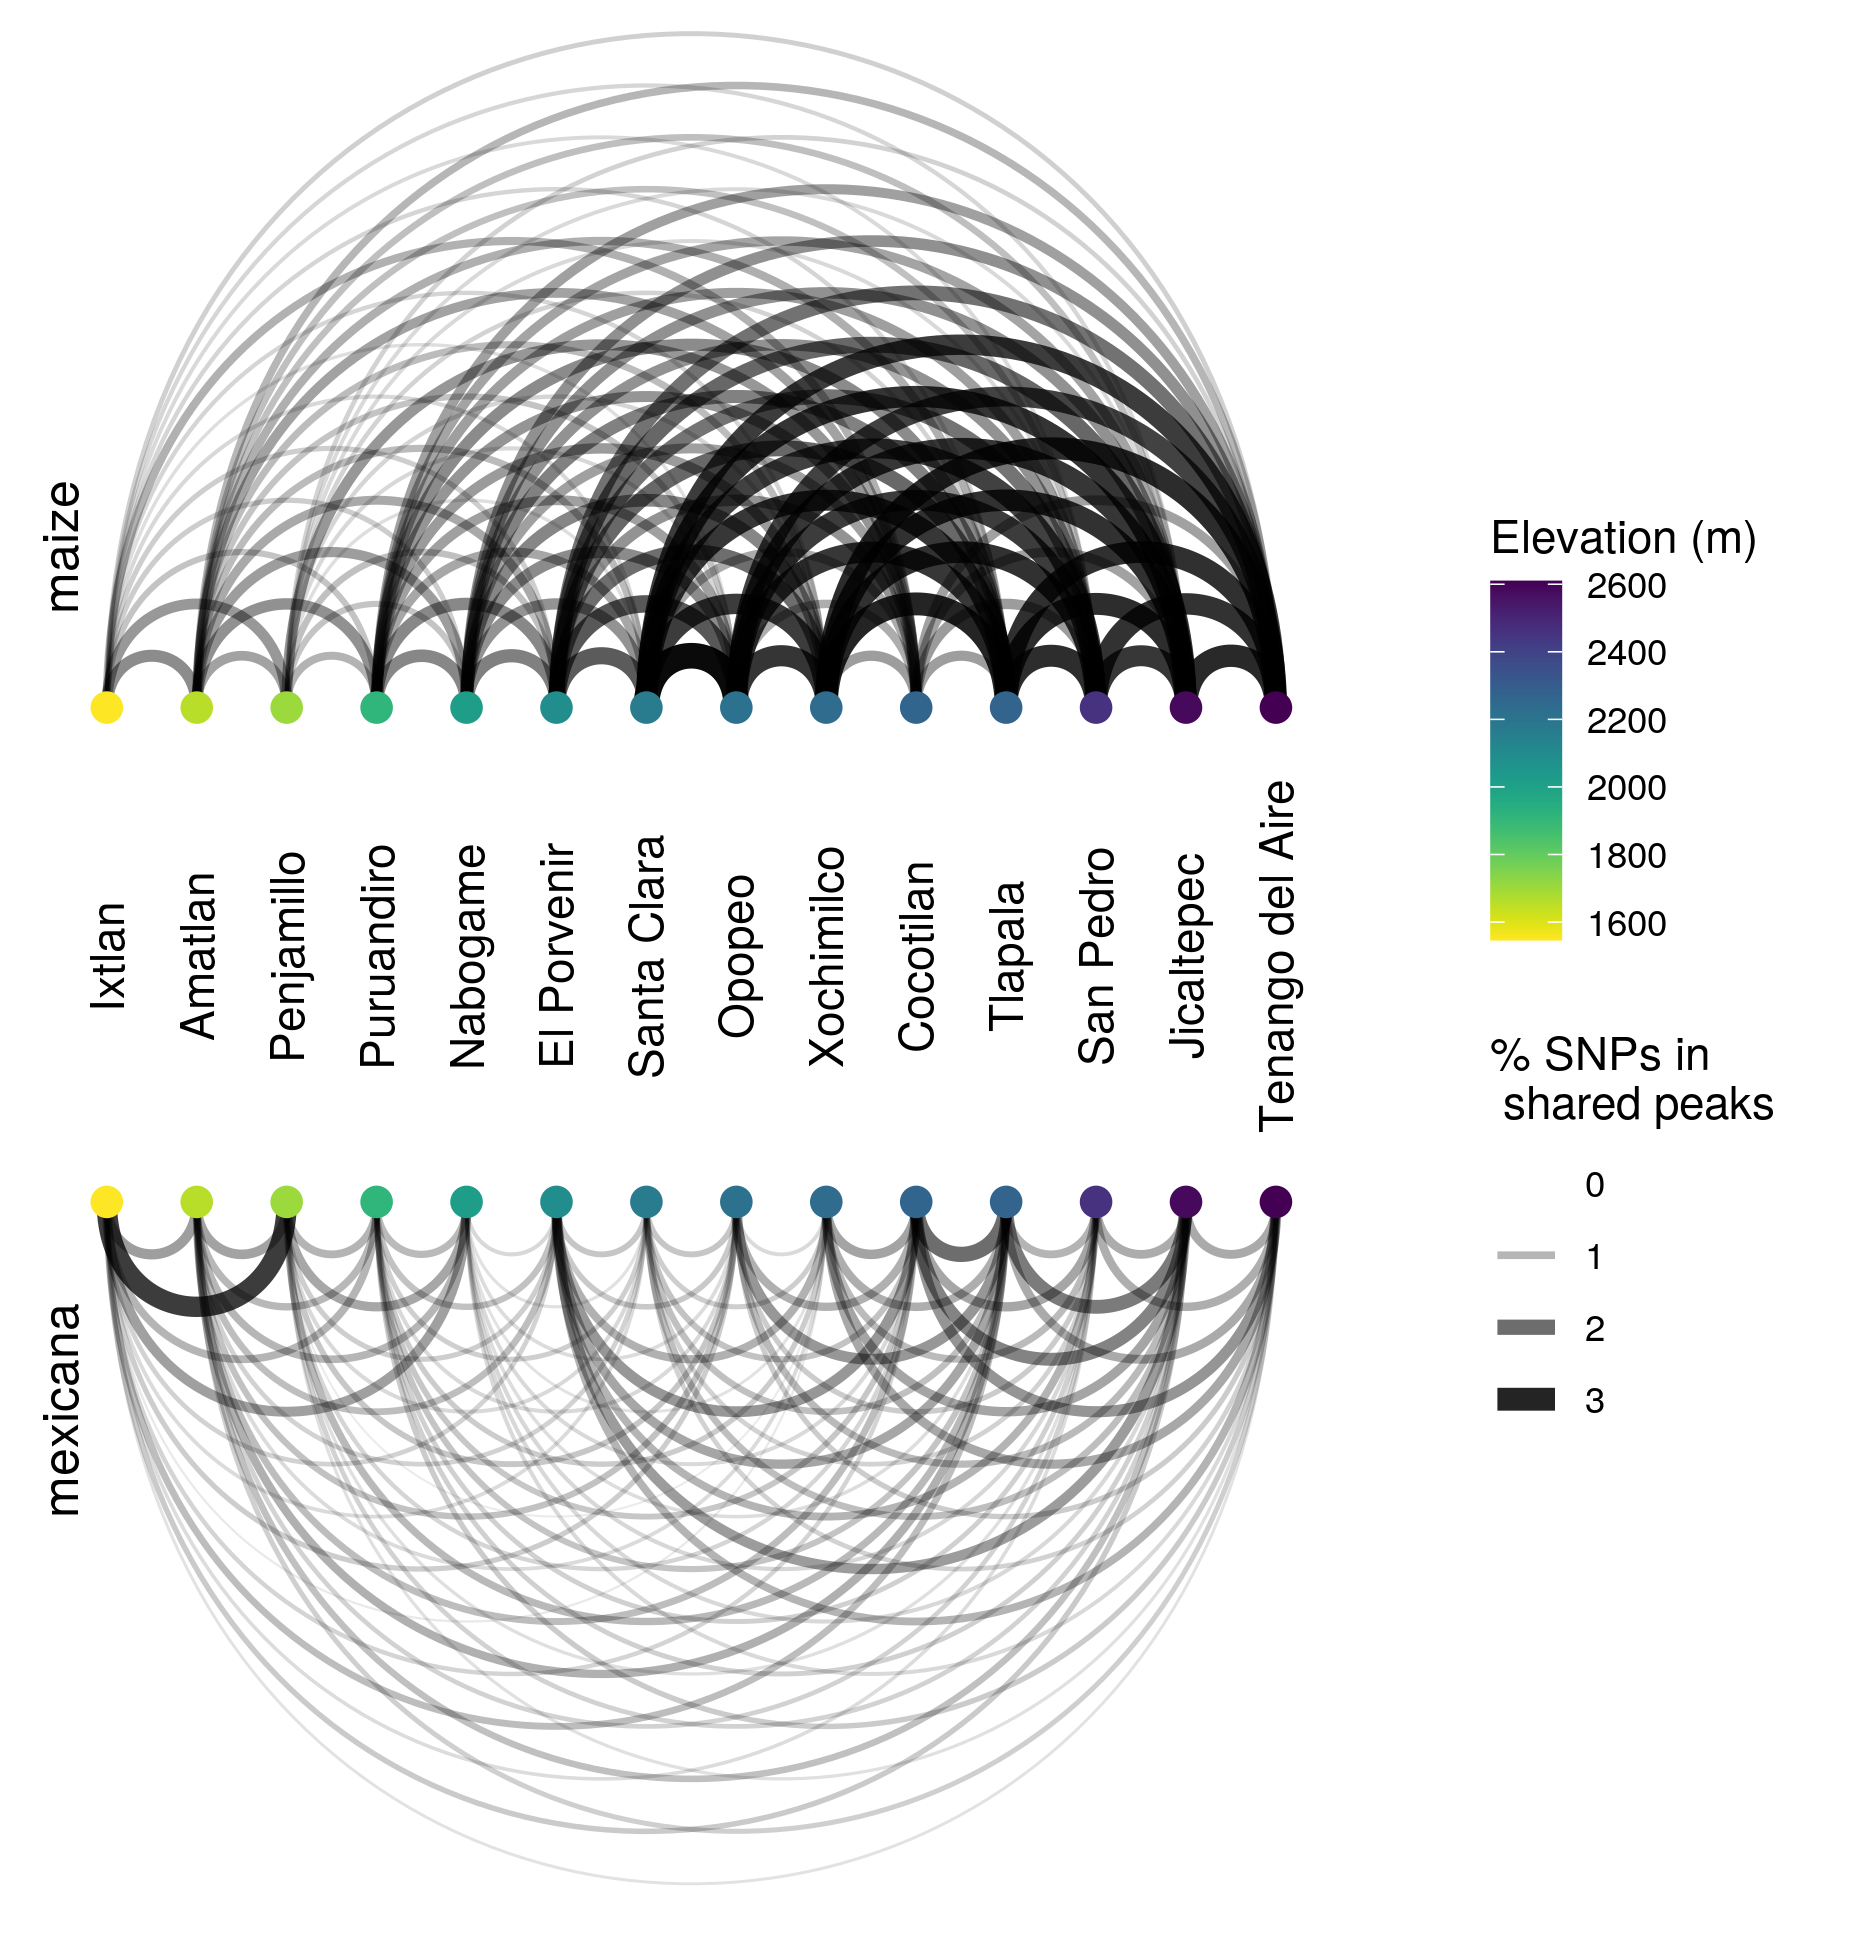
\includegraphics[width=.9\textwidth]{chapter2/figures/network_peak_sharing_data_only.png}
\caption{\color{Gray} \textbf{Introgression peaks shared across populations} Networks for sympatric maize (top) and \mexicana (bottom), where each node is a sampled population labelled by location and ordered by elevation. 
Edges connecting a pair of populations represent the percent of SNPs within shared ancestry peaks (introgressed ancestry $>$ 2 s.d. above each population's mean ancestry). 
Sharing between all pairs of populations exceeds expectations based on multivariate-normal simulations that model genomewide covariance in ancestry.
\ec{The relatively darker thicker lines connecting the high elevation maize populations (except for Cocotilan), indicate that these populations share high introgression peaks at especially high frequencies.}}
\label{network_peaks}
\end{figure}

This lack of local adaptive introgression is perhaps surprising given the genetic structure in \mexicana associated with different ecotypes \cite{Fukunaga:2005fx} and evidence for local adaptation within teosinte across elevation \cite{ Pyhajarvi:2013jc, Fustier:2019, OBrien:2019}. However, \mexicana also has substantial standing variation and we find little evidence for hard sweeps, so one possibility is that local maize and local \mexicana are adapting to the same environment by different available genetic paths, or even the same causal SNP on a different set of haplotype backgrounds. Older introgressed tracts may also offer more accessible paths for maize adaptation, having already purged some of their linked deleterious variation. Additionally, local exitinction and re-colonization by \mexicana is common \cite{Wilkes:1967} and may contribute to a lack of local sourcing of adaptive haplotypes from contemporary \mexicana populations.


\subsection*{Genomewide scan for selection on introgressed ancestry}
We scanned the genome for two types of widespread selection on introgressed ancestry: consistent selection across populations creating an overall excess or deficit of introgression and fitness trade-offs creating steep clines in \mexicana ancestry across elevation. 
We used our MVN simulated ancestry frequencies to set false-discovery-rates for excess and deficits of \textit{mexicana} ancestry as well as steeper than expected slopes between \textit{mexicana} ancestry and elevation \ec{(see Fig \ref{QQ} for model fit)}.

We find several regions with high introgression in both directions that are unlikely to be explained by shared demographic history alone (Fig \ref{genome_scan}). These regions of adaptive introgression ($<$ 5\% FDR) are spread across the genome and cover a small fraction ($<$0.5\%) of the genome in both subspecies. We do not have power to determine if individual genes or regions are barriers to introgression because zero introgressed ancestry is not unusual under our simulated neutral model, given both low genomewide introgression and positive ancestry covariance between admixed populations (Fig \ref{genome_scan}). 

\begin{figure}[h!tb]
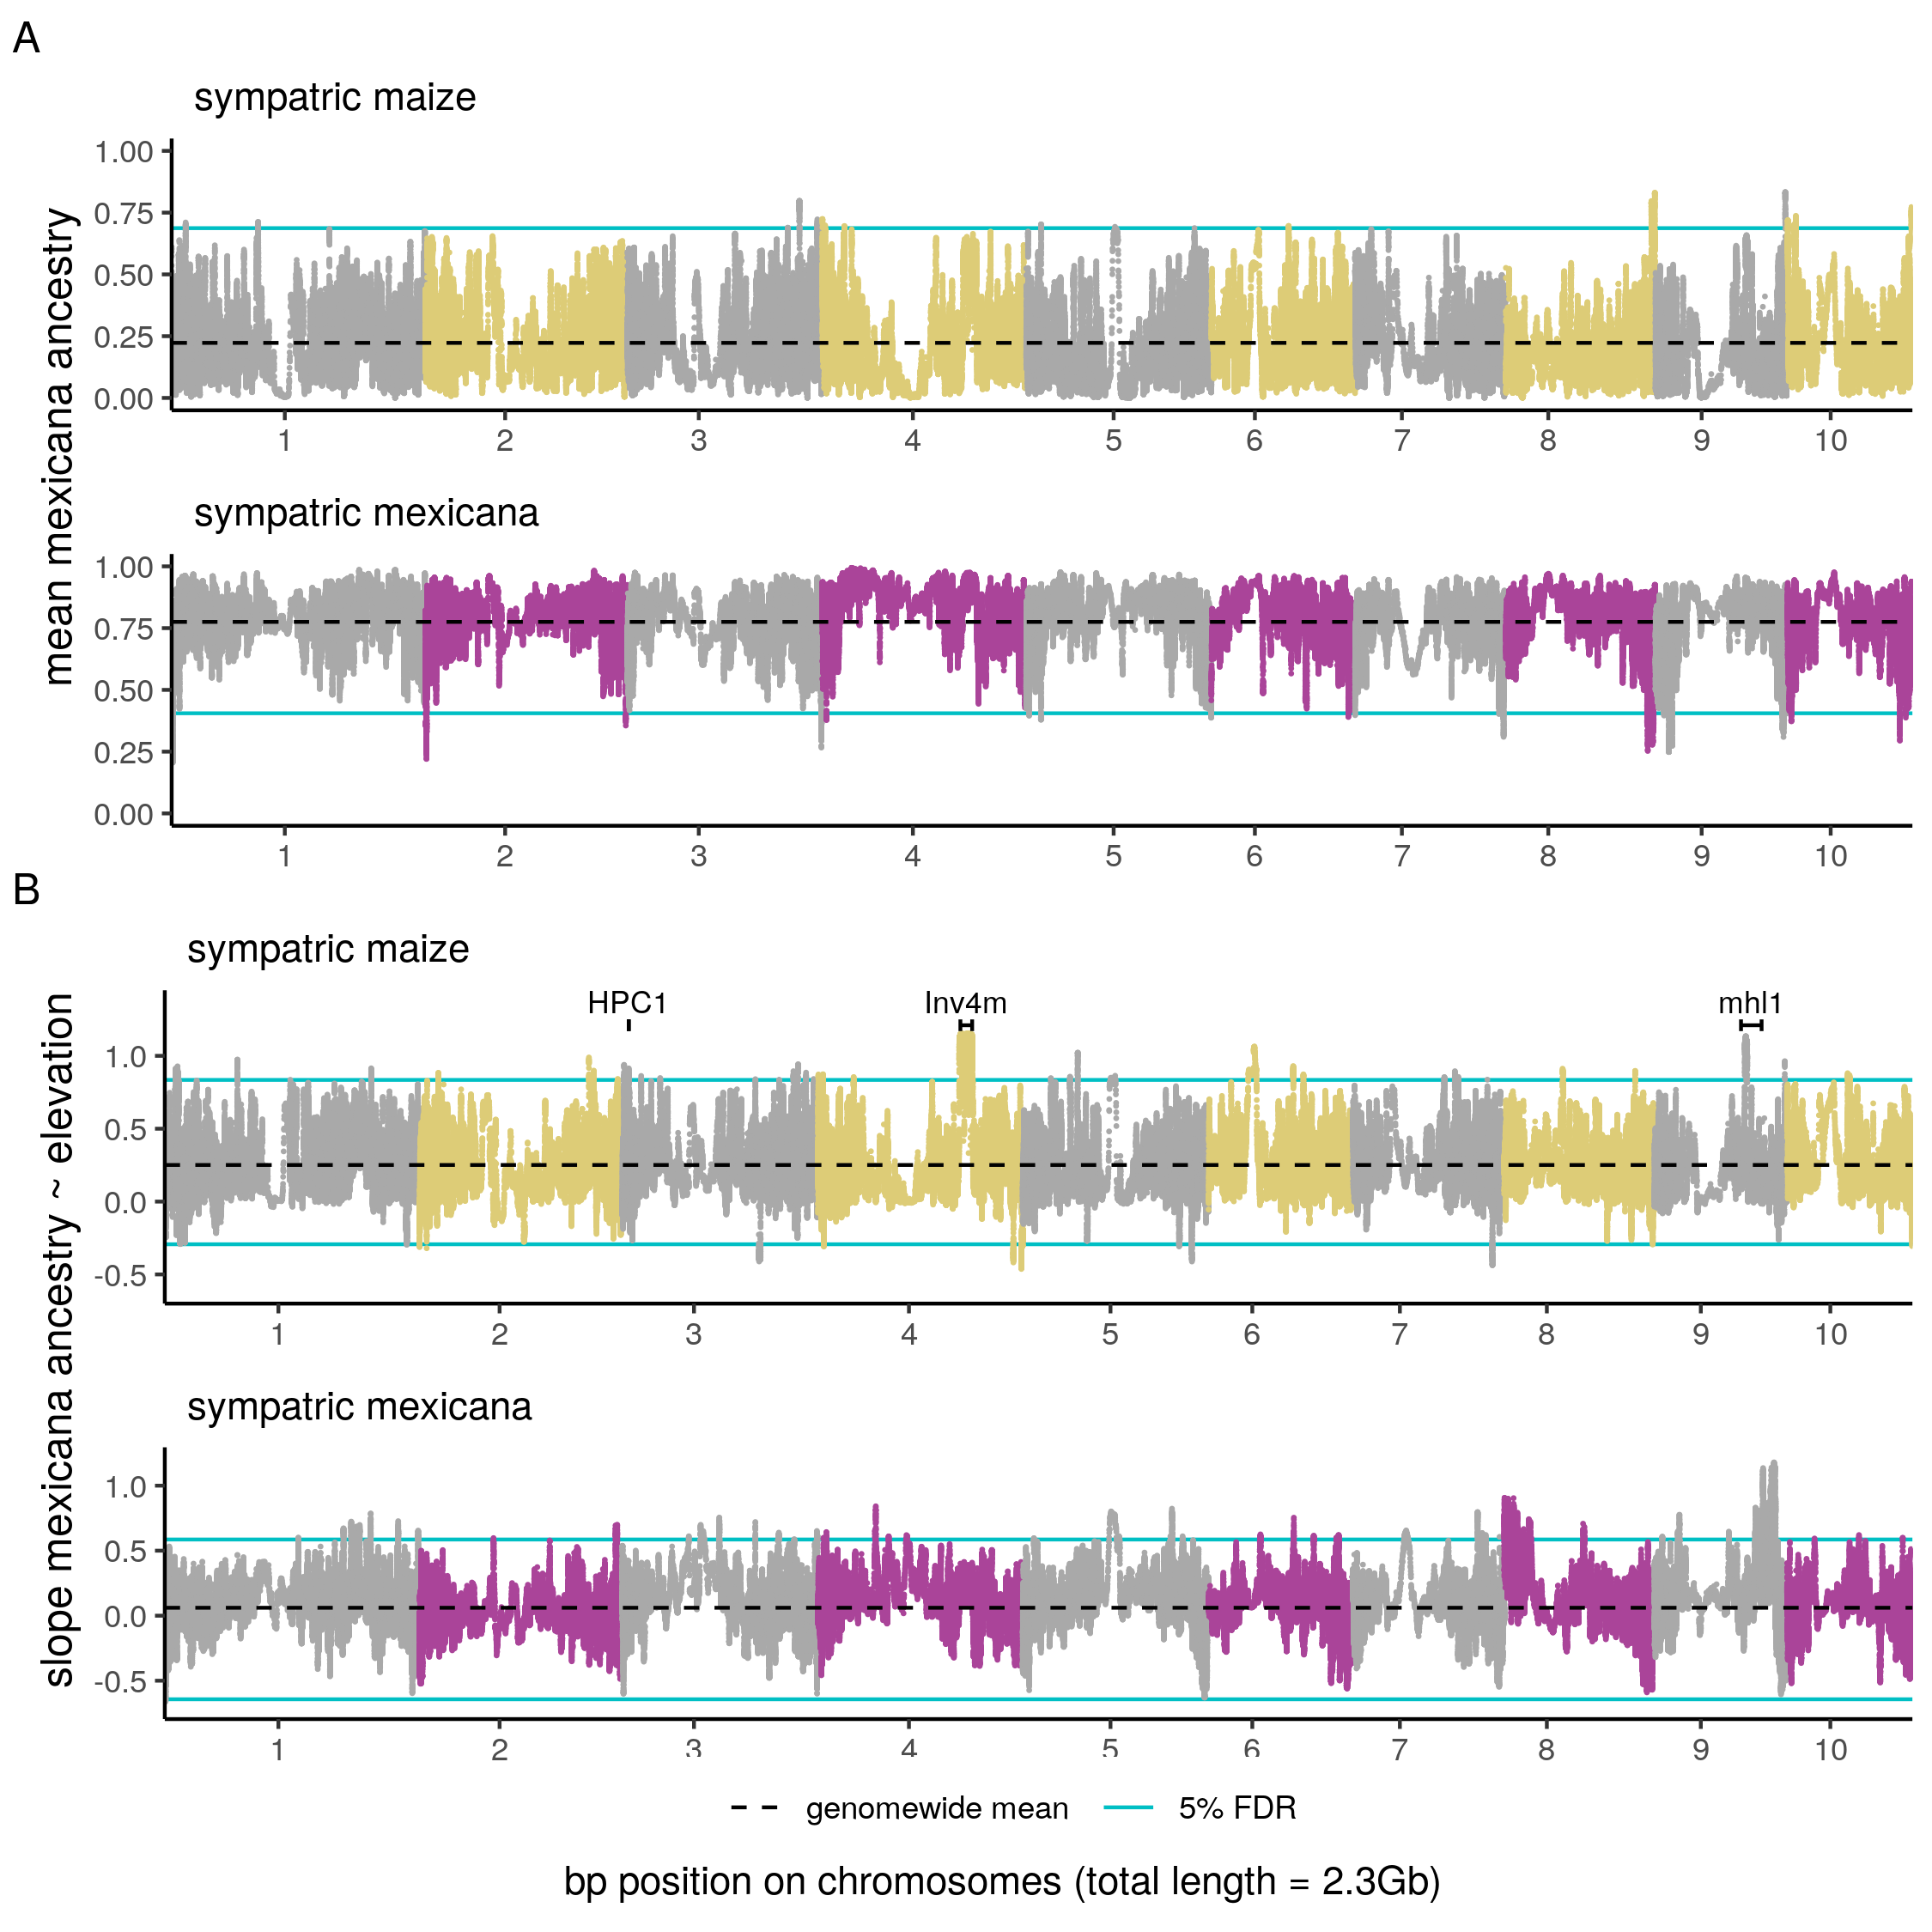
\includegraphics[width=.95\textwidth]{chapter2/figures/multi_maize_mexicana_genome_scan.png}
\caption{\color{Gray} \textbf{Genomewide scan for selection on \textit{mexicana} ancestry}. (A) Mean \mexicana ancestry in sympatric maize  and \mexicana populations. (B) Slope of \mexicana ancestry proportion over a 1 km elevation gain in sympatric maize and \mexicana populations.
In both (A) and (B) the blue lines shows the 5\% false discovery rates, set using multi-variate normal simulations. 
Observing \mexicana ancestry of 0\% in sympatric maize or 100\% in sympatric \mexicana was not unexpected based on simulations.
Positions for \textit{Inv4m} \cite{Pyhajarvi:2013jc} and the \textit{mhl1} locus \cite{Moose_Lauter_Carlson:2004_mhl1} were converted to \ec{the maize reference genome} v4 coordinates using Assembly Converter (ensembl.gramene.org). Chromosome numbers are placed at the centromere midpoint (approximate centromere positions are from \cite{Jiao:2017}).}
\label{genome_scan}
\end{figure}

Additionally, we identify outlier loci across the genome where \mexicana ancestry forms steep clines across elevation (Fig \ref{genome_scan}). 
Our top candidate for strong associations between introgression and elevation in maize is \textit{Inv4m}, a large 14 Mb inversion on chromosome 4 previously identified to have introgressed into high elevation maize landraces \cite{Hufford:2013_crop_wild, Wang:2017, Gonzalez-Segovia:2019, Crow:2020_inv4m}. 
This inversion maintains steep elevational clines within teosintes \cite{Pyhajarvi:2013jc}, overlaps QTLs for leaf pigmentation \cite{Lauter:2004} and macrohairs \cite{Lauter:2004}, and is associated with increased yield in maize at high elevations and decreased yield at low elevations \cite{Crow:2020_inv4m}, but has thus far eluded functional characterization of genes within the inversion \cite{Crow:2020_inv4m}. 


Our second strongest association co-localizes with \textit{macrohairless1} (\textit{mhl1}), a locus on chromosome 9 that controls macrohair initiation on the leaf blade \cite{Moose_Lauter_Carlson:2004_mhl1} and is associated with a major QTL explaining 52\% of macrohair variation between high and low elevation teosinte mapping parents \cite{Lauter:2004}.  
Within teosintes, populations of the lowland ancestor of maize, \textit{parviglumis}, show convergent soft sweeps at the \textit{mhl1} locus not shared by \mexicana \cite{Fustier:2017}. Macrohairs are characteristic highland phenotypes in teosinte and maize and are thought to confer adaptive benefits through insect defence and/or \ec{thermal insulation} \cite{Moya-Raygoza:2016, Lauter:2004}. We identified a 3 Mb outlier region within the larger \textit{mhl1} QTL which we analyzed further using PCA. 
We found three genetic clusters along the first principal component, evidence that an inversion polymorphism (hereafter \textit{Inv9f}) maintains differentiation between maize/\parviglumis and \mexicana haplotypes across this region (Figs \ref{mhl1_slopes}, \ref{mhl1_pca}).
Additionally, principal component two at this inversion separates haplotypes genotyped in maize vs. those genotyped in \mexicana, consistent with the \mexicana allele at this inversion introgressing into maize long enough ago to accumulate maize-specific variation, and subsequently sorting in frequency across contemporary maize populations.

The clinal patterns of admixture that we observe at inversions \textit{Inv4m} and \textit{Inv9f} suggest they contribute to elevation-based adaptation in maize, with variation in their fitness impacts even within the historic elevational range of \mexicana.

While our highest peaks localize
with regions previously associated with characteristic highland phenotypes, many additional outlier regions with steep increases in \mexicana ancestry across elevation have undiscovered associations with local adaptation to elevation. 
Additionally, outliers for steep ancestry slopes across elevation in sympatric \mexicana suggest that introgression from maize into \mexicana may facilitate adaptation in \mexicana to the lower end of its elevational range.

\subsection*{Selection at candidate domestication genes}
We hypothesized that domestication genes will be barriers to introgression bilaterally between maize and \mexicana \cite{Hufford:2013_crop_wild}.
While we do not have power to identify individual outlier genes that have low introgression, we can test for enriched overlap between ‘introgression deserts' and a set of putative domestication genes spread across the genome. 

We examined introgression for a sample of 15 well-characterized domestication genes from the literature (see \nameref{genes_outliers}), and compared them to the regions of the genome with the lowest 5\% introgression genomewide across all sympatric maize or \mexicana populations (‘introgression deserts'). A small but enriched subset of these domestication genes overlap with introgression deserts in sympatric maize (7, P $<$ 0.001) and likewise in sympatric \mexicana (7, P $<$ 0.001).
Among these candidates, we find that \textit{teosinte branched1} (\textit{tb1}), a key transciption factor that regulates branching vs. apical dominance \cite{Doebley_Stec_Gustus:1995_tb1, Doebley_Stec_Hubbard:1997_tb1}, overlaps introgression deserts in both maize and \mexicana, consistent with \textit{tb1}'s role at the top of the domestication regulatory hierarchy \cite{Dong:2019_reg_domestication}.

We also find evidence for reduced introgression into both maize and \mexicana at \textit{teosinte glume architecture1} (\textit{tga1}) \cite{Dorweiler:1993, Wang:2005_tga1} and \textit{brittle endosperm2} (\textit{bt2}) \cite{Whitt:2002_starch}, which are associated with ‘naked' edible grains and starch biosynthesis, respectively. 
Another eight domestication genes \cite{Wills:2018_zagl1, Wills:2013_gt1, Sosso:2015, Vollbrecht:2005_ramosa, Sigmon_Vollbrecht:2010, Lin:2012_shattering, Whitt:2002_starch} have low introgression in one direction only.


Among these, \textit{sugary1} (\textit{su1}) in the starch pathway has low maize ancestry in \mexicana but shows a steep increase in introgressed \mexicana ancestry with elevation in maize ($<$ 5\% FDR), which suggests this gene has pleiotropic effects on non-domestication traits in maize, with fitness trade-offs across elevation. 
\textit{Sugary1} mutations \ec{modify the sweetness, nutrient content and texture of maize kernels (e.g. sweet corn), but} also affect seed germination and emergence at cold temperatures \cite{Trimble:2016_sugary1}, candidate pleiotropic effects that could be more deleterious at higher elevations. 

The remaining four domestication genes do not overlap introgression deserts in either subspecies despite evidence for their role in domestication: \textit{zfl2} (cob rank) \cite{Doebley_Stec:1991, Doebley_Stec:1993, Bomblies_Doebley:2006}, \textit{ba1} (plant architecture) \cite{Gallavotti:2004_ba1}, \textit{ZmSh1-5.1+ZmSh1-5.2} (seed shattering) \cite{Lin:2012_shattering} and \textit{pbf1} (storage protein synthesis) \cite{Wang:1998_pbf}. Despite evidence of introgression at many domestication loci, maize landraces retain all of the classic domestication traits, and \mexicana populations maintain ‘wild' forms. 
Epistasis for domestication traits \cite{Stitzer_Ibarra:2018} could help explain this discrepancy if compensatory effects from other loci contribute to maintaining domestication traits in admixed highland maize, or key domestication alleles segregate at moderate frequencies within \mexicana (but do not have the same phenotypic effects in a teosinte background).

\subsection*{Selection within the flowering time pathway}

Flowering earlier is adaptive in high-elevation environments where days are cooler and there are fewer total growing degree days in a season.
We therefore expect an excess of introgressed \mexicana ancestry at flowering time genes that may contribute to adaptive early flowering in highland maize.
The \mexicana allele at \textit{High PhosphatidylCholine 1} (\textit{HPC1}) has been shown to reduce days to flowering, confers a fitness benefit in maize at higher elevations, and is introgressed in modern flint maize cultivars from Northern Europe and America \cite{Rodriguez-Zapata:2021}. 
Here we show that \textit{HPC1} also overlaps an outlier region with one of the steepest increases in \mexicana ancestry with elevation across sympatric maize populations (+0.91 \mexicana ancestry proportion/km, FDR $<$ 5\%), consistent with a role in adaptive earlier flowering at higher elevations in Mexican landraces. 
\textit{HPC1} has low introgression from maize into sympatric \mexicana across the elevational range of this study, suggesting either that the high-elevation \mexicana allele does not confer fitness tradeoffs in the teosinte background or alternative segregating \mexicana alleles maintain fitness at lower elevations.

We also tested for selection within the flowering time pathway more broadly using a set of 849 candidate flowering time genes \cite{Dong:2012_flowering, Li:2016_flowering}.
Only 1/43 genes from the core flowering time pathway (\textit{ZMM5}) \cite{Dong:2012_flowering} and 15/806 other candidate flowering time genes \cite{Li:2016_flowering} (+/- 20kb) overlap outlier regions with steep increases in \mexicana introgression  with increasing elevation ($<$ 5\% FDR) in sympatric maize, which matches expected overlap by chance ($\sim$2\%,\ P = 0.76).
Thus the steep clinal introgression pattern at \textit{HPC1} in sympatric maize, indicative of strong fitness trade-offs across elevation, is the exception, not the rule, for flowering-time related genes. While for \textit{HPCI} the effect of the \mexicana allele on reducing flowering time has been confirmed by CRISPR \cite{Rodriguez-Zapata:2021}, a limitation for other less-characterized genes is that we simply assume the \mexicana allele reduces flowering time. 
In addition, flowering time is a highly polygenic trait \cite{Buckler:2009}, which could reduce the strength of selection at individual genes with smaller effect sizes than \textit{HPC1} to below what we can detect using steep ancestry clines. 
While it is alternatively possible that \mexicana alleles would show adaptive benefits across the entire range sampled (moderate to high elevation), we find that only 2\ec{/849} candidate flowering time genes overlap high mean \mexicana introgression outliers at a 5\% FDR (P = 0.23).

\section*{Conclusion}
 We conclude that the majority of \mexicana ancestry introgressed into maize over 1000 generations ago and has subsequently been sorted across an elevational gradient, and by selection within individual populations.
 Differentiation of \mexicana haplotypes within maize genomewide ($F_{ST}$) and at individual introgressed outlier loci (e.g. \textit{Inv9f} at the \textit{mhl1} locus (PCA)) corroborate this timeline.
 Despite contemporary observations of \ec{F1} hybrids in the field \cite{Wilkes:1967}, there is little evidence of significant recent gene flow in either direction between sympatric maize-\mexicana population pairs. 
 \ec{Intrinsic genetic incompatibilities and partial temporal isolation (offset flowering times) clearly create an incomplete barrier to gene flow. However, while hybrids are very challenging to identify and weed out from maize fields at early life stages, farmers can easily distinguish between maize and hybrids when choosing which cobs to plant for the next season. In the other direction, hybrids in most locations are expected to be partially temporally isolated from \mexicana and hybrid seeds that do not disarticulate are farmer-dependent for successful dispersal and reproduction, although first-generation backcrosses to \mexicana have been observed \cite{Wilkes:1967}.}

 Consistent with domestication loci acting as barriers to introgression, in both maize and \mexicana an enriched subset of candidate domestication genes overlap ‘introgression deserts.'
 More generally, we find introgressed \mexicana alleles are on average deleterious in maize, but less evidence for a genomewide effect of selection against introgression into \mexicana, possibly because epistasis masks the impact of maize alleles in a \mexicana background \cite{Stitzer_Ibarra:2018}.
 Some loci show exceptional ancestry patterns consistent with selection favoring introgression in multiple populations, especially for \mexicana ancestry in the highest elevation maize. 
 While these shared signatures of adaptive introgression are the most striking, the majority of ancestry peaks are exclusive to a single population.
Despite this signature of geographically-restricted local adaptation from \mexicana ancestry, there is no evidence of local population sources for locally adapted haplotypes at these peaks. Thus both broad and local adaptation of maize throughout the highlands appears to have been driven primarily by the sorting of old introgression.

\section*{Materials and Methods}

\subsection*{Population sampling}
We used maize and \mexicana seed accessions sampled from locations across Mexico in 2008 \cite{Hufford:2013_crop_wild} and currently stored at UC Davis.
We included 14 maize and 14 \mexicana accessions that are paired populations sampled in sympatry from the same locations: Ixtlan*, Amatlan, Penjamillo, Puruandiro*, Nabogame*, El Porvenir*, Santa Clara*, Opopeo*, Xochimilco*, Cocotilan, Tlapala, San Pedro*, Jicaltepec and Tenango del Aire* (see \nameref{population_metadata}). A previous study of crop-wild admixture genotyped different maize and \mexicana individuals from 9 of these locations (marked with *), using the Illumina MaizeSNP50 Genotyping BeadChip \cite{Hufford:2013_crop_wild}. In addition, we chose three population accessions \ec{to sequence as a \mexicana reference panel}: \ec{Puerta Encantada and Malinalco were chosen because they have no record of contemporary maize agriculture nearby and a third population, Amecameca, was added as a complement to these two reference populations because it grows at a higher elevation, beyond the historical range of \parviglumis}.

At each sampling location, multiple ears from maternal plants were collected for seed. 
Population accessions varied in the number of maternal plants with viable seeds. 
When available, we planted multiple seeds within each ear but only randomly selected one individual for sequencing from the plants that successfully germinated in the greenhouse.

\subsection*{DNA extraction and sequencing}
We extracted DNA from leaf tissue and then prepared sequencing DNA libraries using a recently published high-throughput protocol (“Nextera Low Input, Transposase Enabled protocol” \cite{Rowan:2019}) with four main steps: (1) DNA shearing and tagmentation by the Nextera TD enzyme, (2) PCR amplification (Kapa2G Robust PCR kit) and individual sample barcoding (custom 9bp P7 indexing primers) (3) library normalization and pooling, and (4) bead-based clean-up and size-selection of pooled libraries. 
We sequenced the resulting pooled libraries using multiple lanes on Illumina HiSeq 4000 and Novaseq 6000 machines (paired-end 150 bp reads).

To address low sequencing output from some libraries, we re-sequenced 26 libraries (and merged output) and replaced 53 lower-coverage libraries with a higher-coverage library prepared from another seed grown from the same half-sibling family.
We excluded 7 samples from analysis because their final libraries did not yield sufficient sequencing output ($<$0.05x coverage after filtering reads for mapping quality). 
We additionally removed one lane of sequencing (58 samples) from the study after determining a labelling error had occurred for that plate. 

In total, we obtained whole genome sequences for 348 individuals (1.0x average coverage, range: 0.1-2.4x). 
Of these samples, 43 are \mexicana from three allopatric populations, with a total of 34.1x combined coverage. 
The remaining samples are maize and \mexicana from sympatric populations, 262 of which have sufficient coverage for local ancestry inference ($\geq$ 0.5x, 6-12 per sympatric population, see Fig \ref{sequenced_ind_counts}). 
Raw sequencing reads for these low-coverage maize and \mexicana genomes are available at NCBI (PRJNA657016).

\subsection*{Reference genome and recombination map}
We used version 4 of the B73 maize reference genome \cite{Jiao:2017} (Zea\_mays.B73\_RefGen\_v4.dna.toplevel.fa.gz, downloaded 12.18.2018 from Gramene). 
% URL would be better

To find local recombination rates, we converted marker coordinates from a published 0.2 cM genetic map \cite{Ogut:2015df} to the v4 maize genome using Assembly Converter (ensembl.gramene.org). 
We removed any markers that mapped to a different chromosome or out of order on the new assembly, and extended the recombination rate estimates for the most distal mapped windows to the ends of each chromosome. % (Fig \ref{linkage_map})
From this map, we used \textit{approx()} in R (v3.6.2 \cite{R_stats}) to estimate the cM position for any bp position, based on linear interpolation.

\subsection*{Read mapping and filtering}
First, we checked read quality using fastQ Screen (v0.14.0 \cite{Wingett:2018_fastqscreen}) and trimmed out adapter content from raw sequencing reads using the trimmomatic wrapper for snakemake (0.59.1/bio/trimmomatric/pe) \cite{Bolger:2014_trimmomatic}.
We mapped trimmed reads to the maize reference genome using bwa mem (v0.7.17 \cite{Li:2013_bwa}). 
We then sorted reads using SAMtools (v1.9 \cite{Li:2009samtools}), removed duplicates using picardtools (v2.7.1) MarkDuplicates and merged libraries of the same individual sequenced on multiple lanes using SAMtools merge. 
In all subsequent analyses in the methods below we filtered out reads with low mapping scores ($<$ 30) and bases with low base quality scores ($<$ 20).

\subsection*{High-coverage \textit{Tripsacum} genome sequencing}
In addition to low-coverage genomes for maize and \mexicana, we selected a \textit{Tripsacum dactyloides} individual as an outgroup and sequenced it to high coverage. This individual is an outbred ‘Pete' cultivar (rootstock acquired from the Tallgrass Prairie Center, Iowa, USA). We extracted genomic DNA from leaf tissue using the E.Z.N.A.® Plant DNA Kit (Omega Biotek), following manufacturer’s instructions, and then quantified DNA using Qubit (Life Technologies). We prepared a PCR-free Truseq DNA library and sequenced it with an Illumina HiSeq2500 rapid run (paired-end 250 bp reads). We generated a total of 136.53 Gb of sequencing for this individual, available at NCBI (SRR7758238). 
For the following analyses that use \textit{Tripsacum} as an outgroup, we randomly subsampled 50\% of reads using seqtk, for approximately 30x coverage. We mapped reads to the maize reference using the pipeline described above, and additionally capped base quality scores with the ‘extended BAQ' model in SAMtools \cite{Li:2011_BAQ}, which reduces the influence of bases with lower alignment quality.

\subsection*{Additional genomes from published sources}
For an allopatric maize reference population, we used 55 previously published high-coverage maize genomes from \ec{a Tuxpe{\~n}o landrace grown near} Palmar Chico (NCBI: PRJNA616247 \ec{\cite{Chen:2020_maize55, Yang:2019}}). This \ec{maize} population grows \ec{at 983 m}, below the elevational range for \mexicana. 

For a parviglumis reference population, we used 50 previously published high-coverage lowland individuals sampled from the ‘Mound' population at 1,008 m \ec{near} Palmar Chico  \cite{vanHeerwaarden:2010, Yang:2019, Chen:2020_maize55} (NCBI: PRJNA616247, see \nameref{parv50}). We mapped and filtered reads for these individuals using the pipeline described above and capped base quality scores using BAQ.


\subsection*{SNP calling}
We called SNPs using a combined panel of the 348 low-coverage genomes sequenced in this study for sympatric maize, sympatric \mexicana, and allopatric \mexicana, and the 55 high-coverage allopatric maize reference genomes described above. We used ANGSD (v0.932 \cite{Korneliussen:2014_ANGSD}) to identify variant sites with minor allele frequencies $\geq$ 5\% in the total sample based on read counts (‘angsd -doMajorMinor 2 -minMaf 0.05 -doCounts 1 -doMaf 8'). In addition to mapping and base quality filters (‘-minMapQ 30 -minQ 20'), we capped base qualities using the extended per-Base Alignment Quality algorithm (‘-baq 2' \cite{Li:2011_BAQ}) and removed sites that did not have at least 150 individuals with data or had sequencing depth exceeding 2.5x the total sample mean depth. To apply this total depth filter, we estimated mean depth (‘angsd -doCounts 1 -doDepth 1 -maxDepth 10000') for 1000 regions of length 100bp randomly sampled using bedtools (v2.29.0 \cite{Quinlan:2010_bedtools}). 
In total, we identified 52,118,357 SNPs on the assembled chromosomes. In conjunction with SNP calling, we produced genotype likelihoods for each individual at these variant sites using the SAMtools GL method \cite{Li:2009samtools} implemented in ANGSD (‘-GL 1 -doGlf 2').

\subsection*{Global ancestry inference}
To estimate genetic relationships between populations and their genomewide ancestry proportions, we used methods specific to low-coverage data that rely on genotype likelihoods, rather than called genotypes. 
Because these methods are sensitive to SNPs in high linkage disequilibrium (LD), we thinned genotype likelihoods to every 100th SNP ($\sim$4kb spacing) \cite{Tenaillon:2001_LD}.
To confirm that maize and \mexicana subspecies form a major axis of genetic variation in our sample, we estimated the genetic covariance matrix between individuals using PCAngsd (v0.98.2 \cite{Meisner:2018_pcangsd}) and visualized principal components computed using \textit{eigen()} in R. 
We then estimated global ancestry proportions using the same thinned genotype likelihood files as input to NGSAdmix \cite{Skotte:2013_NGSadmix},  using K = 2 clusters. 
Clusters clearly mapped onto the two reference groups, which we used to label the two ancestry components as ‘maize' and ‘\mexicana'.

\subsection*{Local ancestry and timing of admixture}
We inferred local ancestry across the genome using a hidden Markov model that is appropriate for low-coverage data because it models genotype uncertainty down to the level of read counts for all admixed individuals (ancestry\_hmm \cite{CorbettDetig:2017gh}). 
This method relies on allele counts from separate reference populations to estimate allele frequencies for each ancestry. 
Because some of our reference individuals have too low of coverage to accurately call genotypes, we randomly sampled one read per individual to get unbiased frequency estimates for major and minor alleles at each site (‘angsd -doCounts 1 -dumpCounts 3'). 
To maximize ancestry-informativeness of sites in this analysis, we identified SNPs with allele frequency differences of at least 0.3 between subspecies (‘angsd -doMajorMinor 3 -GL 1 -baq 2 -doMaf 1') estimated from at least 44 reference maize and 12 reference \mexicana individuals with sequencing coverage at a site.
We then calculated genetic distances between SNPs \ec{using the maize recombination map} and filtered our enriched variants to \ec{have minimum 0.001 cM spacing between adjacent SNPs} . 

Running ancestry\_hmm jointly infers local ancestry for each individual and the time since admixture. \ec{This HMM method assumes a neutral demographic history in which a constant-size admixed population was formed by a single admixture event $t$ generations in the past, and finds the $t$ that maximize the likelihood of the observed read counts and hidden local ancestry state across each admixed individual's genome. The timing of admixture defines the generations for possible meiotic recombination between ancestry tracts, and therefore scales the transition probabilities between hidden ancestry states. In addition to $t$, the HMM outputs the posterior probabilities for homozygous maize, homozygous \mexicana, and heterozygous ancestry for each individual at every site.} 
\ec{We analysed each} sympatric maize \ec{and} \mexicana population separately, using the population's mean NGSAdmix global ancestry estimate as a prior for mixing proportions, 100 generations as a prior for admixture time (range: 0-10000), an approximate effective population size (Ne) of 10,000 individuals, \ec{genetic positions for each SNP based on the maize linkage map,} and an estimated sequencing base error rate of $3\times10^{-3}$. 
We ran ancestry\_hmm with an optional setting to bootstrap 100 random samples of 1,000-SNP genomic blocks to estimate uncertainty around the estimated generations since admixture \ec{($t$)}. To test the sensitivity of the HMM to our choice of Ne, we re-ran ancestry\_hmm with two other Ne's that differ by an order of magnitude (Ne = 1k, 100k), but did not analyze these results further after finding high correspondence for both local ancestry and timing estimates. 

To get a single point estimate for local ancestry at a site for an individual, \ec{we computed a sum of \mexicana ancestry from the different possible ancestry states, weighted by their posterior probabilities}: \mexicana ancestry proportion = P(homozygous \mexicana) + $\nicefrac{1}{2}$P(heterozygous \ec{maize-\mexicana}). 
In addition, for analyses that require ancestry tract positions, we assumed that the estimated ancestry at a focal site extends halfway to the next site with a local ancestry estimate. 

\subsection*{Diversity within ancestry}
Using \mexicana ancestry estimates from the HMM, we identified high-confidence homozygous ancestry tracts for both maize and \mexicana ancestry (posterior $>$ 0.8). 
We filtered individual bams for reads that overlap these tracks and used the resulting filtered bams to calculate diversity within both maize and 
\mexicana ancestry, separately. 
We estimate diversity using the ANGSD/realSFS framework which is appropriate for low-coverage sequence data it takes into account uncertainty in both genotypes and variant sites. 
We created a concensus fasta sequence for \textit{Tripsacum} (‘angsd -doFasta 2') to use as the ancestral state \ec{for polarizing the unfolded site frequency spectrum in} these analyses.

For each population and ancestry, we estimated the site allele frequencies (‘angsd -doSaf 1 -GL 1') and subsequently estimated the genomewide site frequency spectrum (SFS). We then used this SFS as a prior to estimate within-ancestry pairwise diversity ($\pi$) genomewide from the site allele frequencies (‘realSFS saf2theta'). 

For each pair of populations and ancestry, we additionally used realSFS to estimate the two dimensional SFS from the individual population site allele frequencies genomewide. We then used this 2D SFS as a prior to estimate genomewide within-ancestry $F_{ST}$ between the two populations (‘realSFS fst index -whichFst 1'). 
This call uses Hudson's $F_{ST}$ estimator \cite{Hudson:1992_fst} as parameterized in \cite{Bhatia:2013_fst}.

\subsection*{Effect of local recombination rate on introgressed ancestry}
To estimate the effects of linked selection and recombination rate on genomewide introgression patterns, we compared \mexicana ancestry estimates across genomic quintiles. 
Based on a 0.2 cM-resolution recombination map \cite{Ogut:2015df} for maize, we merged adjacent recombination windows into larger 1 cM non-overlapping windows and calculated each window's mean recombination rate and overlap with coding base pairs (bedr ‘coverage') \cite{R_bedr}. 
We retrieved coding regions (‘CDS') using gene annotations from Ensembl (ensemblgenomes.org, Zea\_mays.B73\_RefGen\_v4.41.chr.gff3.gz, dowloaded 11.6.2018). 
We sorted windows into quintiles for either recombination rate or coding density (bp/cM). 
Each quintile covers approximately $\nicefrac{1}{5}$ of the genome based on physical bp.

\subsection*{i. NGSAdmix estimates}
To estimate ancestry proportions for each recombination rate quintile, we first reduced LD by thinning to 1\% of SNPs (every 100th) and ran NGSAdmix 5 times separately (once per quintile) with K=2 clusters. 
We assigned  ‘maize' and ‘\textit{mexicana}' labels to the ancestry clusters based on majority assignment to the respective allopatric reference panels. 
To bootstrap for uncertainty, we re-sampled 1 cM windows with replacement from each quintile 100 times, and re-ran NGSAdmix on the resulting bootstrap SNP sets. 
Using these results, we calculated 95\% percentile bootstrap confidence intervals for the estimated admixture proportions, and the Spearman's rank correlation between the recombination rate (or coding bp per cM) and admixture proportion ranks for each quintile. 
We also tested for a difference in ancestry slopes with elevation across different recombination rate quintiles by fitting a linear model with an elevation by recombination quintile interaction term: \mexicana ancestry $\sim$ elevation + r + elevation*r. 
Using lm() in R, we fit this model for sympatric maize and sympatric \mexicana separately, treating quintiles as a numeric scale 0-4.

\subsection*{$f_4$ estimates}
In a complementary analysis, we used a ratio of $f_4$ statistics as an alternative method to estimate ancestry proportions by quintile.  \ec{The $f_4$ statistic measures shared genetic drift (allelic covariance) between populations in a phylogeny, due to either shared branch lengths or admixture events in the evolutionary history relating these populations.} 
%and up to a scaling factor is equivalent to the ABBA-BABA statistic. 
\ec{Excess shared drift with one population from a pair of sister populations in the tree is a signature of admixture, analogous to the ABBA-BABA test \cite{Green:2010}, and a ratio of two $f_4$ statistics can be used to quantify the admixture proportion.} 
Assuming the basic phylogenetic tree (((\parviglumis, allopatric maize), allopatric \mexicana), \textit{Tripsacum}) in Fig \ref{f4_tree}, we can estimate $\alpha$, the proportion of ancestry inherited from \mexicana in an admixed population, as follows \cite{Green:2010, Peter:2016}:
$$ \alpha = \frac{f_4(\text{Tripsacum, \parviglumis; X, allopatric maize})}{f_4(\text{Tripsacum, \parviglumis; allopatric \mexicana, allopatric maize)}}.$$
The denominator of this statistic estimates the branch length leading to \parviglumis and allopatric maize that separates these sister subspecies from allopatric \mexicana; the full ratio estimates the proportion of this branch that separates sympatric population X from \parviglumis and allopatric maize, i.e. the \mexicana ancestry in X. 
Because the $f_4$ statistic is sensitive to additional unmodeled admixture within the tree, we limited our allopatric \mexicana group to individuals from just one of the three reference populations (Amecameca), which showed no evidence of admixture in our global ancestry analysis (see Fig \ref{global_anc_multi}).

For each 1 cM window across the genome, we used ANGSD to calculate ABBA-BABA statistics from observed read counts for the 4 populations in the numerator and denominator of the $\alpha$ estimator separately (‘angsd -doabbababa2 1 -remove\_bads 1 -minMapQ 30 -minQ 20 -doCounts 1 -doDepth 1 -maxDepth 10000 -useLast 1 -blockSize 5000000').
From the resulting output files, we summed the negative of the ABBA-BABA numerator (‘Num') and divided by the total number of included sites (‘nSites') across all 1 cM windows within a quintile to get the $f_4$ statistic \cite{Soraggi:2018}. 

We then calculated the Spearman's rank correlation between the recombination rate quintiles and admixture proportion ranks for these quintiles. 
We calculated simple bootstrap confidence intervals for our ancestry estimates and correlations by re-sampling 1 cM windows within quintiles with replacement 10,000 times and re-calculating the $f_4$ ratios and resulting rank correlation across quintiles to construct 95\% percentile confidence intervals. 
We repeated this analysis using quintiles based on coding bp per cM in place of recombination rate (cM/Mbp).

\subsection*{ii. Local ancestry estimates}
We also calculated the Spearman's rank correlation between local recombination rate (or coding bp per cM) and local ancestry proportion at the level of individual 1 cM windows. 
For each window, we averaged local ancestry estimates from the HMM across all individuals within sympatric maize, and separately, sympatric \mexicana. 
We then calculated simple bootstrap confidence intervals for our local ancestry estimates and local recombination rate (or coding bp per cM) by re-sampling 1 cM windows across the genome with replacement 10,000 times and re-calculating the rank correlation across windows to construct 95\% percentile confidence intervals.


\subsection*{Local ancestry simulations}

%Here, the demographic history (and therefore independence) of admixed populations was previously unknown because of %potential long-distance (and in the case of maize, likely human-facilitated) gene flow between populations.

We simulated \mexicana ancestry population frequencies using a multivariate-normal null model:

$$mexicana\ \text{ancestry} \sim \text{MVN}(\vec{\alpha}, K)$$
where $\vec{\alpha}$ is the vector of mean \mexicana ancestry frequencies genomewide for each sympatric population and $K$ is the empirical ancestry variance-covariance matrix relating these 14 populations. 
The diagonal entries of the K matrix capture the expected variation in local ancestry across the genome within populations due to drift and random sampling. 
The off-diagonals capture ancestry covariances between populations created by shared gene flow and drift post-admixture: at loci where one population has an excess of introgression, other admixed populations with shared demographic history will also tend to have an excess of introgression.

To construct K, we calculated the covariance in ancestry between each pair of populations \textit{i} and \textit{j}  using all \textit{L} loci with local ancestry calls genomewide:

\begin{align*}
K[i, j] = \frac{1}{L} \sum_{l=1}^{L} (Anc_{i,l} - \alpha_i)(Anc_{j,l} - \alpha_j).
\end{align*}

Above, $Anc_{i,l}$ and $Anc_{j,l}$ are local ancestry frequencies at a locus \textit{l} while $\alpha_i$ and $\alpha_j$ are the mean local ancestry frequencies across the genome for populations \textit{i} and \textit{j}.

For sympatric maize and sympatric \mexicana separately, we calculated the empirical K matrix between populations from all 14 sympatric locations, and then took 100,000 independent draws from their MVN distribution, thereby simulating \mexicana ancestry for all populations at 100,000 unlinked loci. 
Because ancestry frequencies are bounded at [0,1] but normal distributions are not, we truncated any simulated values outside of this range.

\subsection*{Introgression peaks shared between populations}
To characterize introgression peak sharing between individual populations, we defined ‘ancestry peaks' as sites where a population has over 2 standard deviations more introgressed ancestry than the genomewide mean. 
We counted the number of peaks that are shared between all pairs and combinations of populations. 
To compare these results to our null model, we also counted the number of introgression peaks shared by populations in our simulated dataset, using the 2 s.d. cutoff set by the empirical data to define peaks.

Because \mexicana ancestry shows significant diversity, we additionally characterized diversity for \mexicana ancestry peaks introgressed into maize. 
For all introgressed ancestry outlier regions in a focal maize population, we used ANGSD to estimate pairwise diversity within the population ($\pi$) and differentiation ($F_{ST}$) between the focal sympatric maize populations and their local sympatric \mexicana population.
We focused on the \mexicana ancestry within peaks by limiting our diversity estimates to only include high-confidence homozygous \mexicana ancestry tracts (posterior $>$ 0.8). 
For these analyses, we pooled information across outlier peaks, but distinguish between introgression peaks exclusive to the focal population and introgression peaks shared between the focal population and at least 3 other sympatric maize populations.
We used global estimates of the SFS and 2D SFS as priors to estimate $\pi$ and $F_{ST}$ for the subsets of the genome within introgression peaks, and otherwise followed the same methods listed above in ‘Diversity within ancestry'. 

\subsection*{Genomewide scan for ancestry outliers}

For sympatric maize and \mexicana separately, we calculated the mean \mexicana ancestry across all individuals at a locus, and fit a linear model using lm() in R to estimate the slope of \mexicana ancestry frequencies for sympatric populations across elevation (km): \mexicana ancestry $\sim$ elevation. We then repeated these summary statistics for every locus with an ancestry call in the empirical data and each simulated locus in the MVN simulated data.

We calculated 5\% false-discovery-rate (FDR) cutoffs for high and low \mexicana ancestry using the Benjamini-Hochberg method \cite{Benjamini_Hochberg:1995} and simulation results to estimate the expected frequency of false-positives under our null MVN model (one-tailed tests). 
We repeated this approach to identify outlier loci with steep positive (or negative) slopes for \mexicana ancestry across elevation at a 5\% FDR. 

\subsection*{Test for reduced introgression at domestication genes}
%\subsection*{Test for reduced introgression at domestication loci}
%We used the 31 landraces from Wang \cite{Wang:2017} to identify selective sweep patterns indicative of loci involved in the domestication of maize. 
%Specifically, we mapped reads from each accession to the maize v4 reference and called variants using the GATK germline variant call best practices to call SNPs from the alignments. We then used RAiSD to characterize sweeps from these genotypes.
%RAiSD was run under default settings and the only modification we made was to use the script mop (https://github.com/RILAB/mop) to quantify unmappable reads for each RAisD window and adjusted the window size in the RAiSD output to reflect the mappable bases, as opposed to the physical number of bases in each window.

To test whether domestication genes are unusually resistant to introgression, we first defined ‘introgression deserts' as regions with the lowest 5\% of introgression genomewide across all sympatric maize (or, separately, sympatric \mexicana) populations. We then looked up v4 coordinates on Ensembl.org for genes associated with maize domestication in the literature (\nameref{genes_outliers}), and used bedtools ‘intersect' to identify which of these genes $\pm 20$ kb overlap introgression deserts. To test for significance, we randomly shuffled the gene positions across the genome (bedtools ‘shuffle') 1000 times and re-calculated overlap with introgression deserts for each permuted data set.

\subsection*{Test for selection within the flowering time pathway}
We identified a list of 48 core flowering time pathway genes from the literature \cite{Dong:2012_flowering}, and a broader list of 905 flowering time candidate genes \cite{Li:2016_flowering, Dong:2012_flowering}. 
From the combined set, we included 849 total genes (43 core pathway) which we were able to localize on assembled autosomes of the v4 reference genome using MaizeGDB gene cross-reference files \cite{Portwood:2019_MaizeGDB}.
We counted the number of genes $\pm 20$ kb that intersected with outlier regions for steep increases in \mexicana introgression with elevation (and, separately, high \mexicana introgression) in sympatric maize populations ($<$ 5\% FDR) using bedtools ‘intersect', then tested for significance by repeating this analysis with 1000 randomly shuffled gene positions.


\subsection*{Analysis pipeline and data visualization}

We constructed and ran bioinformatics pipelines using snakemake (v.5.17.0 \cite{Koester_Rahmann:2012_snakemake}) within a python conda environment (v3.6). 
We analyzed and visualized data in R (v3.6.2 \cite{R_stats}) using the following major packages: tidyverse (v1.3.0 \cite{R_tidyverse}), viridis (v0.5.1 \cite{R_viridis}), bedr (v1.0.7 \cite{R_bedr}), boot (v.1.3\_25 \cite{R_boot, Davison_Hinkley:1997_boot}), gridExtra (v2.3 \cite{R_gridExtra}), ggupset (v0.3.0 \cite{R_ggupset}) and tidygraph (1.2.0 \cite{R_tidygraph}). 
All scripts can be found on our gitHub repository, https://github.com/ecalfee/hilo, which also includes a full list of software and versions (see envs/environment.yaml).


\section*{Acknowledgments}
The authors would like to acknowledge funding from NSF award number 1546719 to JRI and GC. This work was also supported by the National Institute of General Medical Sciences of the National Institutes of Health (NIH R01 GM108779 and R35 GM136290, awarded to GC). We thank Pesach Lubinsky for collecting the seeds sequenced in this study. We also want to thank the Coop and Ross-Ibarra labs, and the HILO and Zeavolution working groups for helpful feedback on this work.


\medskip

\section*{Associated Publication}
An earlier version of Chapter 2 was posted as a preprint to BioRxiv on March 5, 2021. This preprint will be updated with a link to the final peer-reviewed article upon publication: \newline

Calfee E, Gates D, Lorant A, Perkins TA, Coop G, Ross-Ibarra J. Selective sorting of ancestral introgression in maize and teosinte along an elevational cline. BioRxiv. 2021;\\
doi:10.1101/2021.03.05.434040

%This is where your bibliography is generated. Make sure that your .bib file is actually called library.bib
%\bibliography{chapter2/library}


%This defines the bibliographies style. Search online for a list of available styles.
%\bibliographystyle{plos2015}

\newpage
\section*{Supporting Information}

%\newpage

\paragraph*{Table 2.1}
\label{population_metadata}
{\bf Population metadata.} 
\begin{table}[ht]
\centering
\begin{tabular}{llllllll}
\hline
Subspecies & Group & Location & Country & \makecell[lt]{Elev.\\ (m)} & Latitude & Longitude & Accession \\
\hline
\mexicana & allopatric & \makecell[lt]{Puerta\\ Encantada} & Mexico & 1658 & 18.9725 & -99.0298 & RIMME0033 \\
\mexicana & allopatric & Malinalco & Mexico & 1887 & 18.9531 & -99.503 & RIMME0020 \\
\mexicana & allopatric & Amecameca & Mexico & 2467 & 19.139 & -98.7733 & RIMME0022 \\
maize & sympatric & Ixtlan & Mexico & 1547 & 20.1683 & -102.373 & RIMMA0371 \\
maize & sympatric & Amatlan & Mexico & 1658 & 18.9719 & -99.0551 & RIMMA0369 \\
maize & sympatric & Penjamillo & Mexico & 1705 & 20.1176 & -101.93 & RIMMA0361 \\
maize & sympatric & Puruandiro & Mexico & 1915 & 20.1076 & -101.49 & RIMMA0370 \\
maize & sympatric & Nabogame & Mexico & 2020 & 26.2465 & -106.915 & RIMMA0360 \\
maize & sympatric & El Porvenir & Mexico & 2094 & 19.6789 & -100.64 & RIMMA0363 \\
maize & sympatric & Santa Clara & Mexico & 2173 & 19.4184 & -101.642 & RIMMA0362 \\
maize & sympatric & Opopeo & Mexico & 2213 & 19.4181 & -101.613 & RIMMA0368 \\
maize & sympatric & Xochimilco & Mexico & 2237 & 19.2861 & -99.0827 & RIMMA0374 \\
maize & sympatric & Cocotilan & Mexico & 2269 & 19.2244 & -98.8427 & RIMMA0367 \\
maize & sympatric & Tlapala & Mexico & 2272 & 19.2351 & -98.8368 & RIMMA0365 \\
maize & sympatric & San Pedro & Mexico & 2459 & 19.0886 & -98.4935 & RIMMA0372 \\
maize & sympatric & Jicaltepec & Mexico & 2587 & 19.3764 & -99.6303 & RIMMA0366 \\
maize & sympatric & \makecell[lt]{Tenango\\ del Aire} & Mexico & 2609 & 19.1197 & -99.5896 & RIMMA0373 \\
\mexicana & sympatric & Ixtlan & Mexico & 1547 & 20.1683 & -102.373 & RIMME0029 \\
\mexicana & sympatric & Amatlan & Mexico & 1658 & 18.9719 & -99.0551 & RIMME0027 \\
\mexicana & sympatric & Penjamillo & Mexico & 1705 & 20.1176 & -101.93 & RIMME0019 \\
\mexicana & sympatric & Puruandiro & Mexico & 1915 & 20.1076 & -101.49 & RIMME0028 \\
\mexicana & sympatric & Nabogame & Mexico & 2020 & 26.2465 & -106.915 & RIMME0018 \\
\mexicana & sympatric & El Porvenir & Mexico & 2094 & 19.6789 & -100.64 & RIMME0021 \\
\mexicana & sympatric & Santa Clara & Mexico & 2173 & 19.4184 & -101.642 & RIMME0034 \\
\mexicana & sympatric & Opopeo & Mexico & 2213 & 19.4181 & -101.613 & RIMME0026 \\
\mexicana & sympatric & Xochimilco & Mexico & 2237 & 19.2861 & -99.0827 & RIMME0035 \\
\mexicana & sympatric & Cocotilan & Mexico & 2269 & 19.2244 & -98.8427 & RIMME0025 \\
\mexicana & sympatric & Tlapala & Mexico & 2272 & 19.2351 & -98.8368 & RIMME0023 \\
\mexicana & sympatric & San Pedro & Mexico & 2459 & 19.0886 & -98.4935 & RIMME0030 \\
\mexicana & sympatric & Jicaltepec & Mexico & 2587 & 19.3764 & -99.6303 & RIMME0024 \\
\mexicana & sympatric & \makecell[lt]{Tenango\\ del Aire} & Mexico & 2609 & 19.1197 & -99.5896 & RIMME0031 \\
\hline 
\end{tabular} 
\end{table}

\newpage

\paragraph*{Table 2.2}
\label{parv50}
{\bf Parviglumis SRA IDs.} 
\begin{table}[ht]
\centering
\begin{tabular}{llll}
\hline
Run & Isolate & Run (cont.) & Isolate (cont.) \\
\hline
SRR11448802 & PC\_M59\_ID1 & SRR13207117 & PC\_J01\_ID1 \\
SRR11448838 & PC\_I05\_ID1 & SRR11448791 & PC\_N48\_ID1 \\
SRR11448793 & PC\_N13\_ID1 & SRR11448812 & PC\_L08\_ID1 \\
SRR11448797 & PC\_N09\_ID1 & SRR11448834 & PC\_I50\_ID1 \\
SRR11448799 & PC\_N07\_ID1 & SRR13207120 & PC\_O08\_ID1 \\
SRR11448800 & PC\_N04\_ID1 & SRR11448794 & PC\_N11\_ID1 \\
SRR11448803 & PC\_M58\_ID1 & SRR11448804 & PC\_M15\_ID1 \\
SRR11448805 & PC\_M05\_ID1 & SRR11448807 & PC\_L56\_ID1 \\
SRR11448809 & PC\_L14\_ID1 & SRR13207095 & PC\_J08\_ID1 \\
SRR11448811 & PC\_L12\_ID1 & SRR13207116 & PC\_O59\_ID1 \\
SRR11448814 & PC\_K60\_ID1 \\
SRR11448816 & PC\_K54\_ID1 \\
SRR11448818 & PC\_K02\_ID1 \\
SRR11448819 & PC\_J51\_ID1 \\
SRR11448820 & PC\_J50\_ID1 \\
SRR11448823 & PC\_J13\_ID1 \\
SRR11448824 & PC\_J12\_ID1 \\
SRR11448825 & PC\_J10\_ID1 \\
SRR11448827 & PC\_J04\_ID1 \\
SRR11448830 & PC\_I58\_ID1 \\
SRR11448832 & PC\_I52\_ID1 \\
SRR11448836 & PC\_I08\_ID1 \\
SRR11448837 & PC\_I06\_ID1 \\
SRR13207106 & PC\_J07\_ID1 \\
SRR13207118 & PC\_O51\_ID1 \\
SRR13207119 & PC\_O10\_ID1 \\
SRR13207121 & PC\_N60\_ID1 \\
SRR13207122 & PC\_N58\_ID1 \\
SRR13207123 & PC\_N57\_ID1 \\
SRR13207124 & PC\_N56\_ID1 \\
SRR13207125 & PC\_N14\_ID1 \\
SRR13207126 & PC\_N10\_ID1 \\
SRR13207127 & PC\_L48\_ID1 \\
SRR13207128 & PC\_I53\_ID1 \\
SRR13207129 & PC\_I11\_ID1 \\
SRR13207130 & PC\_L10\_ID1 \\
SRR13207131 & PC\_L06\_ID1 \\
SRR13207138 & PC\_K55\_ID1 \\
SRR13207149 & PC\_J48\_ID1 \\
SRR13207160 & PC\_J14\_ID1 \\
% \\
% \\
% \\
% \\
% \\
% \\
% \\
% \\
% \\
% \\
\hline 
\end{tabular} 
\end{table}


\newpage

\paragraph*{Table 2.3}
\label{spearmans_rho_ngsadmix}
{\bf Spearman's rank correlation between \mexicana ancestry (NGSAdmix) and recombination rate (or coding bp per cM) quintiles}
% latex table generated in R 3.6.2 by xtable 1.8-4 package
% Thu Feb  4 23:14:59 2021
\begin{table}[ht]
\centering
\begin{tabular}{llrrr}
  \hline
group & feature & Spearman's $\rho$ & 2.5\% & 97.5\% \\ 
  \hline
allopatric maize & recombination rate (cM/Mb) & -0.36 & -0.90 & 0.67 \\ 
  allopatric mexicana & recombination rate (cM/Mb) & 0.40 & 0.10 & 1.00 \\ 
  sympatric maize & recombination rate (cM/Mb) & 1.00 & 0.85 & 1.00 \\ 
  sympatric mexicana & recombination rate (cM/Mb) & 1.00 & 0.90 & 1.00 \\ 
  allopatric maize & coding bp per cM & 0.62 & -0.30 & 1.00 \\ 
  allopatric mexicana & coding bp per cM & -0.40 & -0.90 & -0.20 \\ 
  sympatric maize & coding bp per cM & -1.00 & -1.00 & -0.85 \\ 
  sympatric mexicana & coding bp per cM & -0.90 & -1.00 & -0.80 \\ 
   \hline
\end{tabular}
\end{table}


\paragraph*{Table 2.4}
\label{spearmans_rho_f4_sympatric_maize_pop22}
{\bf Spearman's rank correlation between ancestry ($f_4$ ratio) and recombination rate (or coding bp per cM) quintiles in sympatric maize}
% latex table generated in R 3.6.2 by xtable 1.8-4 package
% Thu Feb  4 23:22:58 2021
\begin{table}[ht]
\centering
\begin{tabular}{llrrr}
  \hline
group & feature & Spearman's $\rho$ & 2.5\% & 97.5\% \\ 
  \hline
sympatric maize & recombination rate (cM/Mb) & 1.00 & 0.30 & 1.00 \\ 
  sympatric maize & coding bp per cM & -0.90 & -1.00 & 0.10 \\ 
   \hline
\end{tabular}
\end{table}


\paragraph*{Table 2.5}
\label{tbl_elev_r_interaction_5}
{\bf Ancestry by elevation and recombination rate quintile.} Best-fitting linear models for ancestry proportion predicted by an elevation by recombination rate interaction: \mexicana ancestry $\sim$ elevation + r + elevation*r. Here, r is the recombination rate quintile, treated as numeric [0-4]. This model only uses ancestry estimates for sympatric individuals and is fit separately for maize and \mexicana samples.
% latex table generated in R 3.6.2 by xtable 1.8-4 package
% Thu Feb  4 23:14:59 2021
\begin{table}[ht]
\centering
\begin{tabular}{llrrrr}
  \hline
group & term & estimate & std.error & statistic & p.value \\ 
  \hline
sympatric maize & intercept & -0.122 & 0.027 & -4.512 & 7.67E-06 \\ 
  sympatric maize & elevation (km) & 0.083 & 0.013 & 6.596 & 9.01E-11 \\ 
  sympatric maize & r quintile & -0.110 & 0.011 & -9.896 & 1.50E-21 \\ 
  sympatric maize & elevation*r quintile & 0.074 & 0.005 & 14.399 & 8.27E-41 \\ 
  sympatric mexicana & intercept & 0.270 & 0.035 & 7.710 & 3.35E-14 \\ 
  sympatric mexicana & elevation (km) & 0.270 & 0.016 & 16.590 & 4.52E-54 \\ 
  sympatric mexicana & r quintile & 0.119 & 0.014 & 8.309 & 3.57E-16 \\ 
  sympatric mexicana & elevation*r quintile & -0.045 & 0.007 & -6.735 & 2.94E-11 \\ 
   \hline
\end{tabular}
\end{table}


\paragraph*{Table 2.6}
\label{spearmans_rho_f4_sympatric_mexicana_pop22}
{\bf Spearman's rank correlation between ancestry ($f_4$ ratio) and recombination rate (or coding bp per cM) quintiles in sympatric \mexicana}
{% latex table generated in R 3.6.2 by xtable 1.8-4 package
% Thu Feb  4 23:23:05 2021
\begin{table}[ht]
\centering
\begin{tabular}{llrrr}
  \hline
group & feature & Spearman's $\rho$ & 2.5\% & 97.5\% \\ 
  \hline
sympatric mexicana & recombination rate (cM/Mb) & 1.00 & 0.80 & 1.00 \\ 
  sympatric mexicana & coding bp per cM & -1.00 & -1.00 & -0.90 \\ 
   \hline
\end{tabular}
\end{table}
}

\paragraph*{Table 2.7}
\label{spearmans_rho_local_ancestry}
{\bf Spearman's rank correlation between mean \mexicana local ancestry and recombination rate (or coding bp per cM) at 1 cM genomic window resolution.} Confidence intervals are constructed using the percentile method and 10,000 bootstrap replicates created by randomly re-sampling 1 cM windows within quintiles.
% latex table generated in R 3.6.2 by xtable 1.8-4 package
% Fri Feb  5 00:04:33 2021
\begin{table}[ht]
\centering
\begin{tabular}{llrrr}
  \hline
group & feature & Spearman's $\rho$ & 2.5\% & 97.5\% \\ 
  \hline
sympatric maize & recombination rate (cM/Mb) & 0.011 & -0.039 & 0.062 \\ 
  sympatric maize & coding bp per cM & 0.014 & -0.038 & 0.066 \\ 
  sympatric \mexicana & recombination rate (cM/Mb) & -0.473 & -0.512 & -0.432 \\ 
  sympatric \mexicana & coding bp per cM & 0.339 & 0.292 & 0.384 \\ 
   \hline
\end{tabular}
\end{table}


\newpage

%\paragraph*{Table 2.8}
%\label{genes_outliers}
%{\bf Domestication genes and overlap with low introgression regions.}
% latex table generated in R 3.6.2 by xtable 1.8-4 package
% Thu Mar  4 20:55:46 2021
\begin{sidewaystable}[ht]

\paragraph*{Table 2.8}
\label{genes_outliers}
{\bf Domestication genes and overlap with low introgression regions.}
\newline
\\
%\begin{table}[p]
\centering
\begin{tabular}{llllll}
  \hline
gene & phenotype & references & maize v4 coordinates & \makecell[bl]{minimum\\ introgression
\\ in maize} & \makecell[tl]{minimum\\ introgression\\
 in mexicana} \\ 
  \hline
zagl1 & ear size & \cite{Wills:2018_zagl1} & 1:4959131-5014850 & 0.012* & 0.264 \\ 
  gt1 & prolificacy & \cite{Wills:2013_gt1} & 1:23605801-23647370 & 0.004* & 0.106 \\ 
  ZmSh1-1 & seed shattering & \cite{Lin:2012_shattering} & 1:228660490-228705551 & 0.356 & 0.038* \\ 
  tb1 & branching & \cite{Doebley_Stec_Gustus:1995_tb1, Doebley_Stec_Hubbard:1997_tb1, Dong:2019_reg_domestication} & 1:270533676-270574776 & 0.001* & 0.06* \\ 
  zfl2 & cob rank  & \cite{Doebley_Stec:1991, Doebley_Stec:1993, Bomblies_Doebley:2006} & 2:12894091-12937068 & 0.113 & 0.271 \\ 
  pbf1 & \makecell[tl]{storage protein\\ synthesis} & \cite{Wang:1998_pbf} & 2:158122366-158176919 & 0.092 & 0.084 \\ 
  ra2 & \makecell[tl]{inflorescence\\ architecture} & \cite{Vollbrecht:2005_ramosa} & 3:12138280-12179065 & 0.144 & 0.046* \\ 
  ba1 & plant architecture & \cite{Gallavotti:2004_ba1} & 3:185994629-186035264 & 0.33 & 0.154 \\ 
  su1 & starch biosynthesis & \cite{Whitt:2002_starch} & 4:43090569-43139167 & 0.445 & 0.017* \\ 
  tga1 & 'naked' grains & \cite{Dorweiler:1993, Wang:2005_tga1} & 4:46330597-46375118 & 0.036* & 0.007* \\ 
  bt2 & starch biosynthesis & \cite{Whitt:2002_starch} & 4:61295575-61341350 & 0.027* & 0.016* \\ 
  \makecell[tl]{ZmSh1-5.1+\\ZmSh1-5.2} & seed shattering & \cite{Lin:2012_shattering} & 5:16630307-16676707 & 0.105 & 0.175 \\ 
  sweet4c & \makecell[tl]{sugar transport\\ and seed size} & \cite{Sosso:2015} & 5:130767030-130809864 & 0.014* & 0.163 \\ 
  ae1 & starch biosynthesis & \cite{Whitt:2002_starch} & 5:172392995-172450415 & 0.436 & 0.059* \\ 
  ra1 & \makecell[tl]{inflorescence\\ architecture} & \cite{Vollbrecht:2005_ramosa, Sigmon_Vollbrecht:2010} & 7:113552410-113592937 & 0.006* & 0.176 \\ 
   \hline
\end{tabular}
\\
 * lowest 5\% introgression genomewide ('introgression desert')
\end{sidewaystable}
%\end{table}
 % table title is within this .tex
\clearpage


%\begin{figure}[h!]
\begin{figure}[ht]
	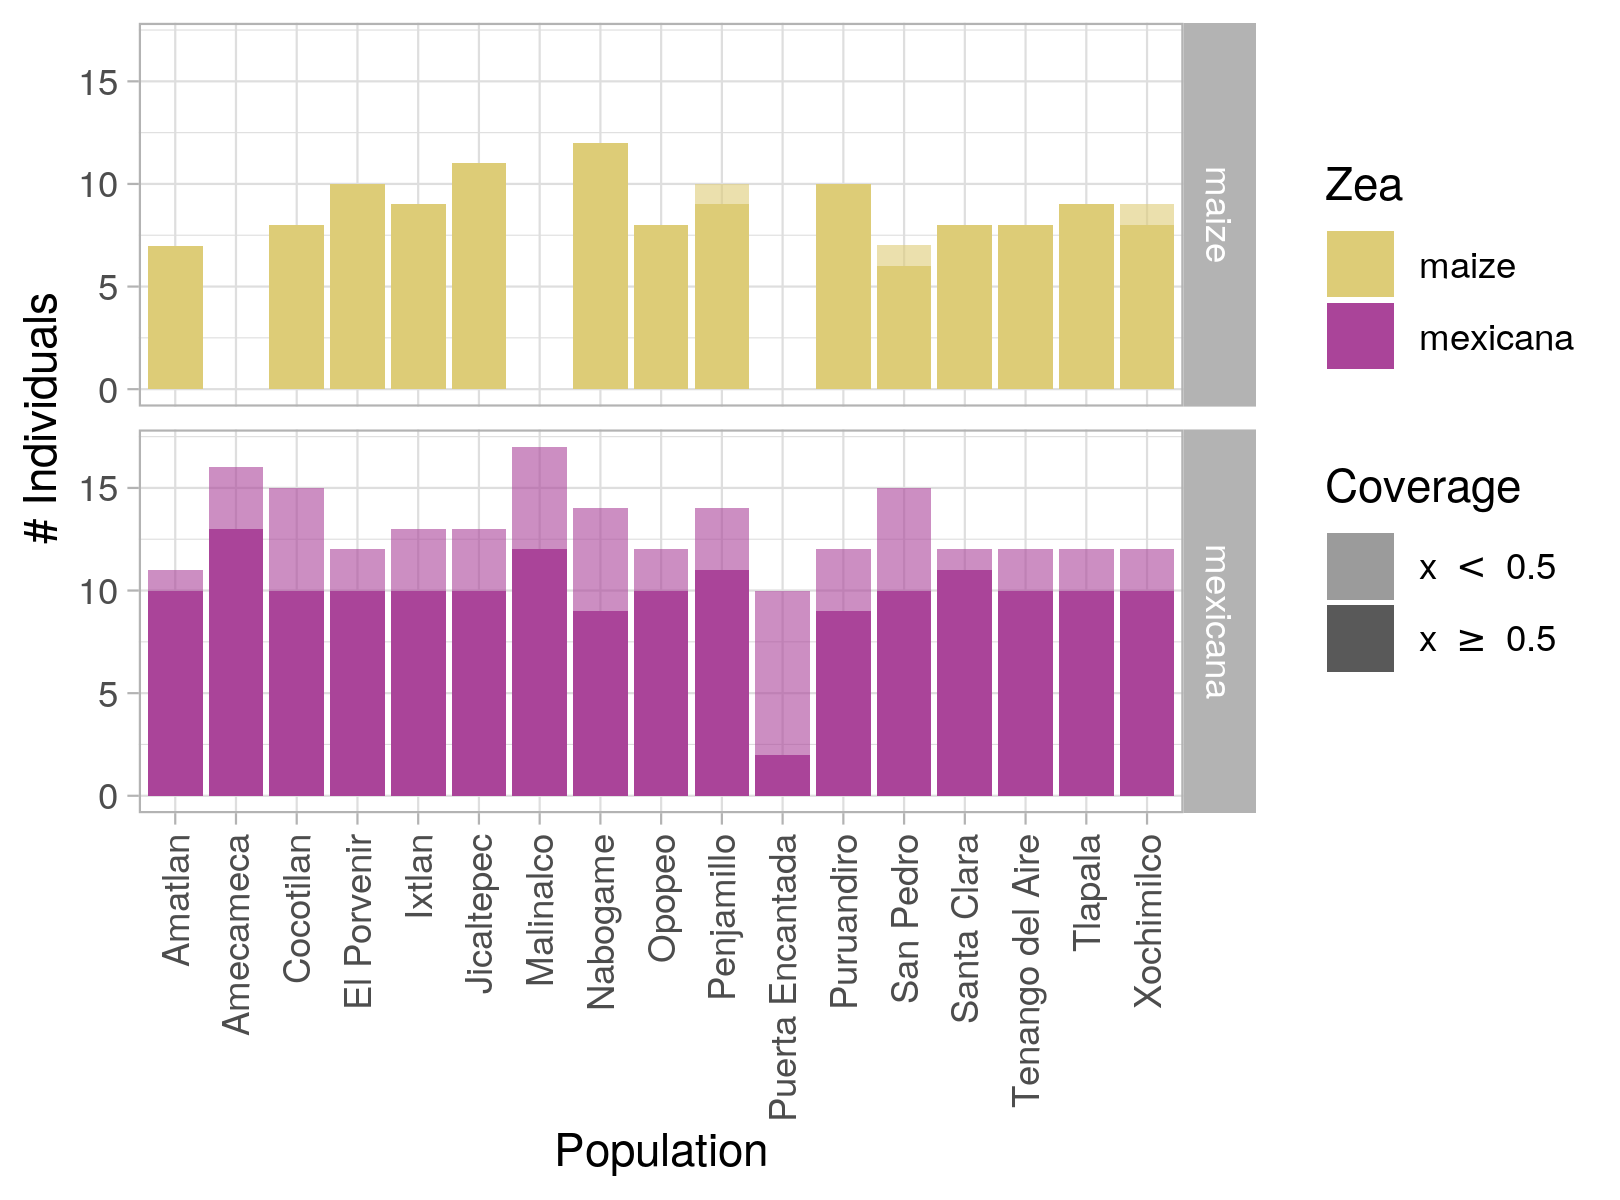
\includegraphics[width=\textwidth]{chapter2/figures/p_seq_counts.png}
	\caption{\color{Gray} \textbf{Number of individuals sequenced per location}. Number of maize (top) and \textit{mexicana} (bottom) individuals sequenced by this study with minimum 0.05x WGS coverage. Amecameca, Malinalco and Puerta Encantada have no paired maize samples and are used as a reference panel for \textit{mexicana} ancestry. For sympatric maize and \textit{mexicana}, only individuals meeting a more stringent 0.5x coverage threshold (shown in darker shading) are included in analyses based on local ancestry inference.}
	\label{sequenced_ind_counts}
\end{figure}

\begin{figure}[ht]
%\begin{figure}[ht]
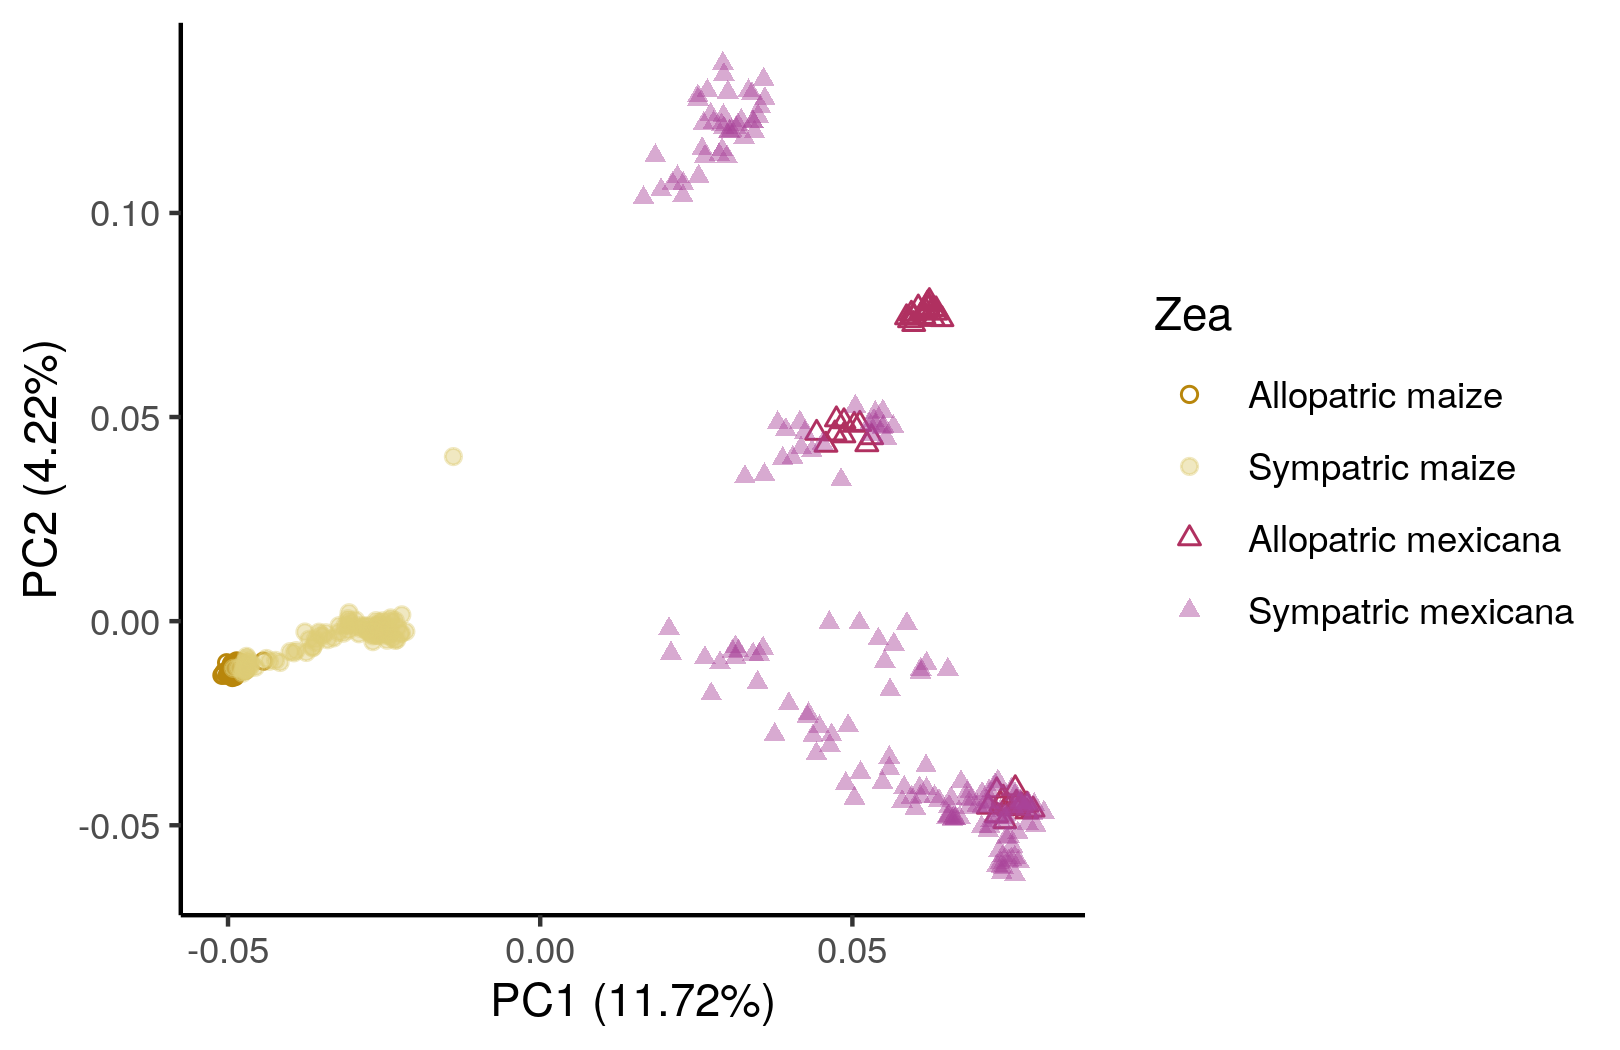
\includegraphics[width=\textwidth]{chapter2/figures/HILO_MAIZE55_pca.png}
\caption{\color{Gray} \textbf{PCA}. First and second principal components from the genomewide genetic covariance matrix relating sympatric and allopatric maize and \mexicana individuals (PCAngsd). PC1 separates maize and \mexicana subspecies while PC2 differentiates genetic clusters within \mexicana.}
\label{pca_maize_mex}
\end{figure}

%\begin{figure}[p]
\begin{figure}[ht]
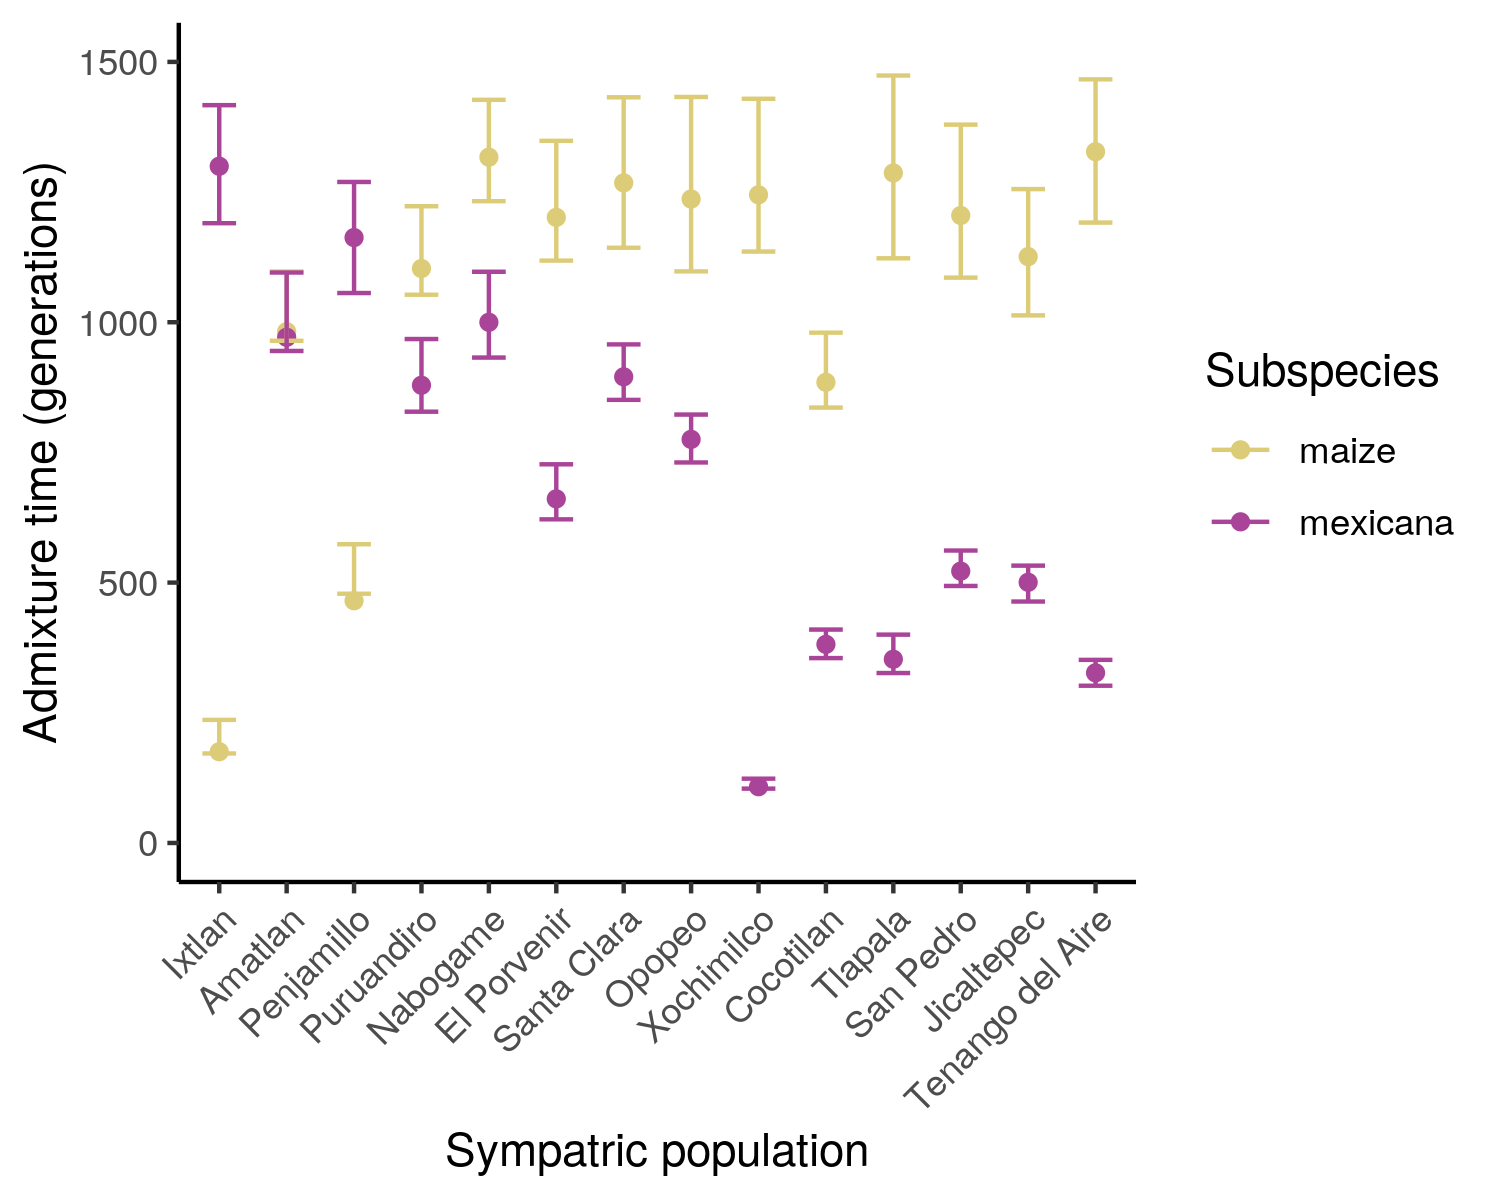
\includegraphics[width=\textwidth]{chapter2/figures/admix_times_Ne10000_yesBoot.png}
\caption{\color{Gray} \textbf{Time since admixture}. Estimated generations since admixture under a single-pulse model for each sympatric maize and \mexicana population, with 95\% percentile confidence intervals based on 100 bootstrap samples of genomic blocks (1,000 SNPs per block). Estimates and bootstraps were produced during ancestry\_hmm model fitting for local ancestry inference. Populations are ordered left to right by increasing elevation.}
\label{time_admix}
\end{figure}

\begin{figure}[ht]
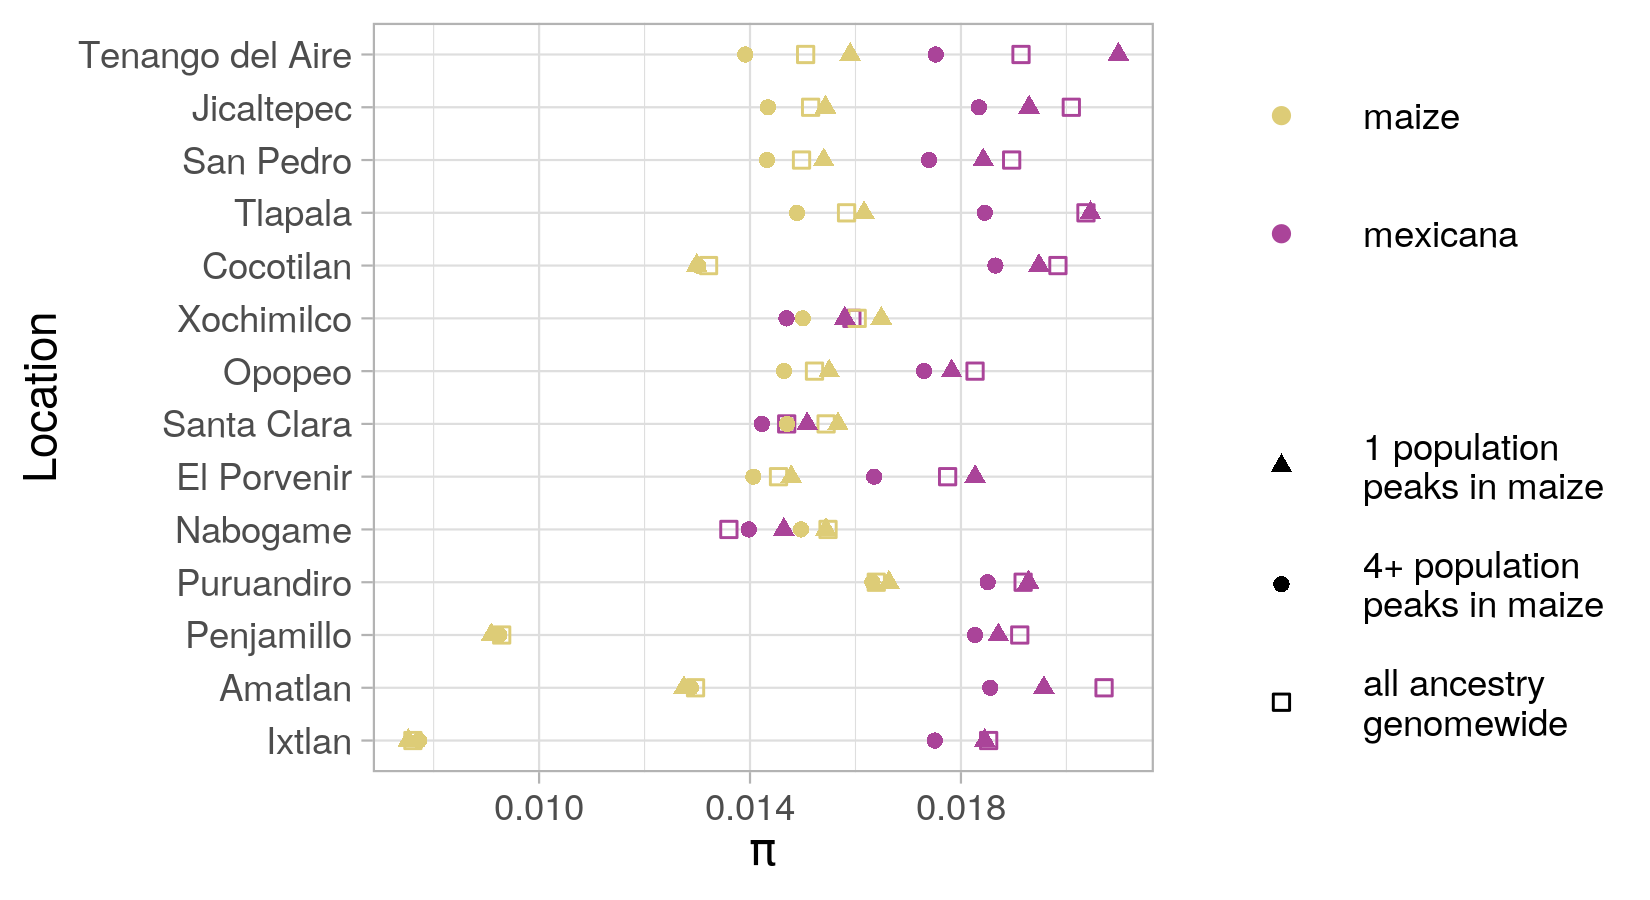
\includegraphics[width=\textwidth]{chapter2/figures/pi_within_mexicana_ancestry_peaks.png}
\caption{\color{Gray} \textbf{Diversity ($\pi$) within \mexicana ancestry} Each point summarises pairwise genetic diversity ($\pi$) for genomic regions with high-confidence homozygous \mexicana ancestry, calculated separately for the maize and \mexicana populations at each sampled location. Within-\mexicana ancestry $\pi$ is calculated and plotted separately for three subsets of the genome: introgression peaks ($>$ 2 s.d. above the mean) found in the focal maize population only, peaks shared between the focal maize and at least 3 other maize populations, and a genomewide estimate.}
\label{pi_mexicana_ancestry_peaks}
\end{figure}

\begin{figure}[ht]
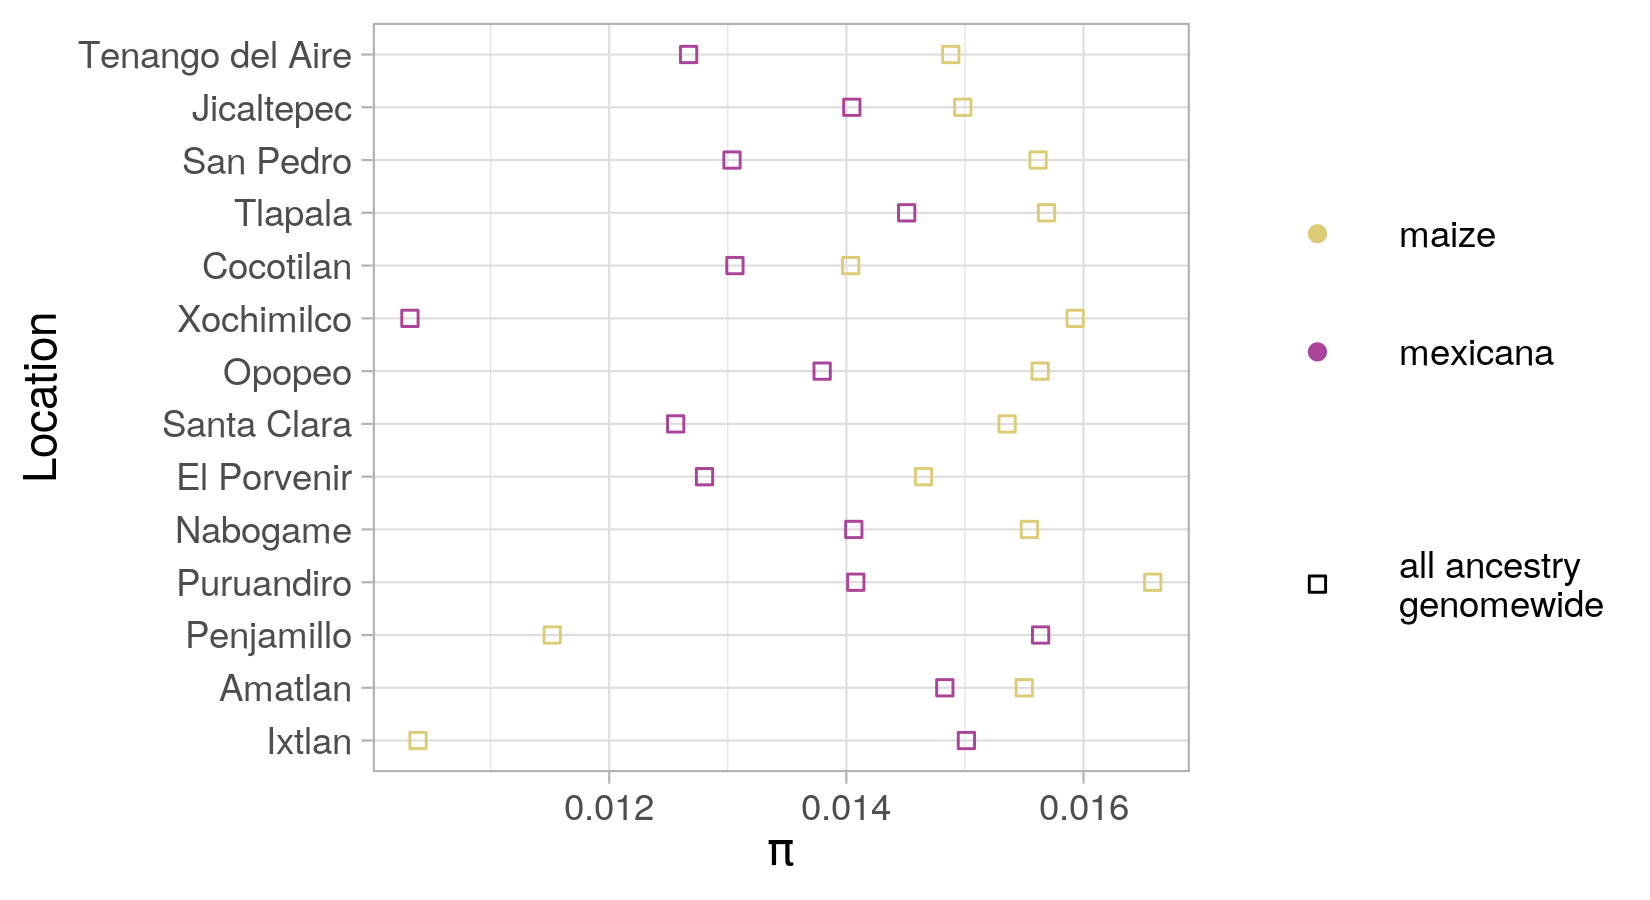
\includegraphics[width=\textwidth]{chapter2/figures/pi_within_maize_ancestry.png}
\caption{\color{Gray} \textbf{Diversity ($\pi$) within maize ancestry} Each point summarises pairwise genetic diversity ($\pi$) for regions genomewide with high-confidence homozygous \mexicana ancestry, calculated separately for the maize and \mexicana populations at each sampled location.}
\label{pi_maize_ancestry}
\end{figure}

%\begin{figure}[p]
\begin{figure}[ht]
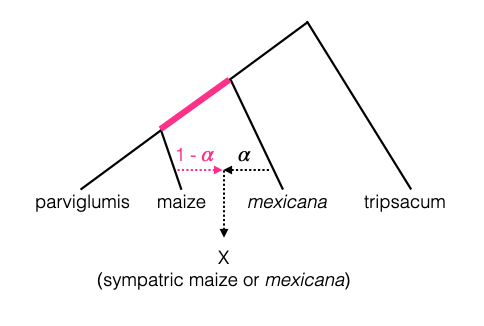
\includegraphics[width=\textwidth]{chapter2/figures/tree_f4_stats.png}
\caption{\color{Gray} \textbf{Population tree} Phylogenetic tree assumed when estimating the ratio of $f_4$ statistics. The pink branch represents the shared drift between maize and \parviglumis that is introduced to the focal sympatric population via admixture of proportion $1 - \alpha$. We used only plants from the Amecameca site in our \mexicana reference group for this analysis because that site showed no evidence of previous admixture.}
\label{f4_tree}
\end{figure}

%\begin{figure}[p]
\begin{figure}[ht]
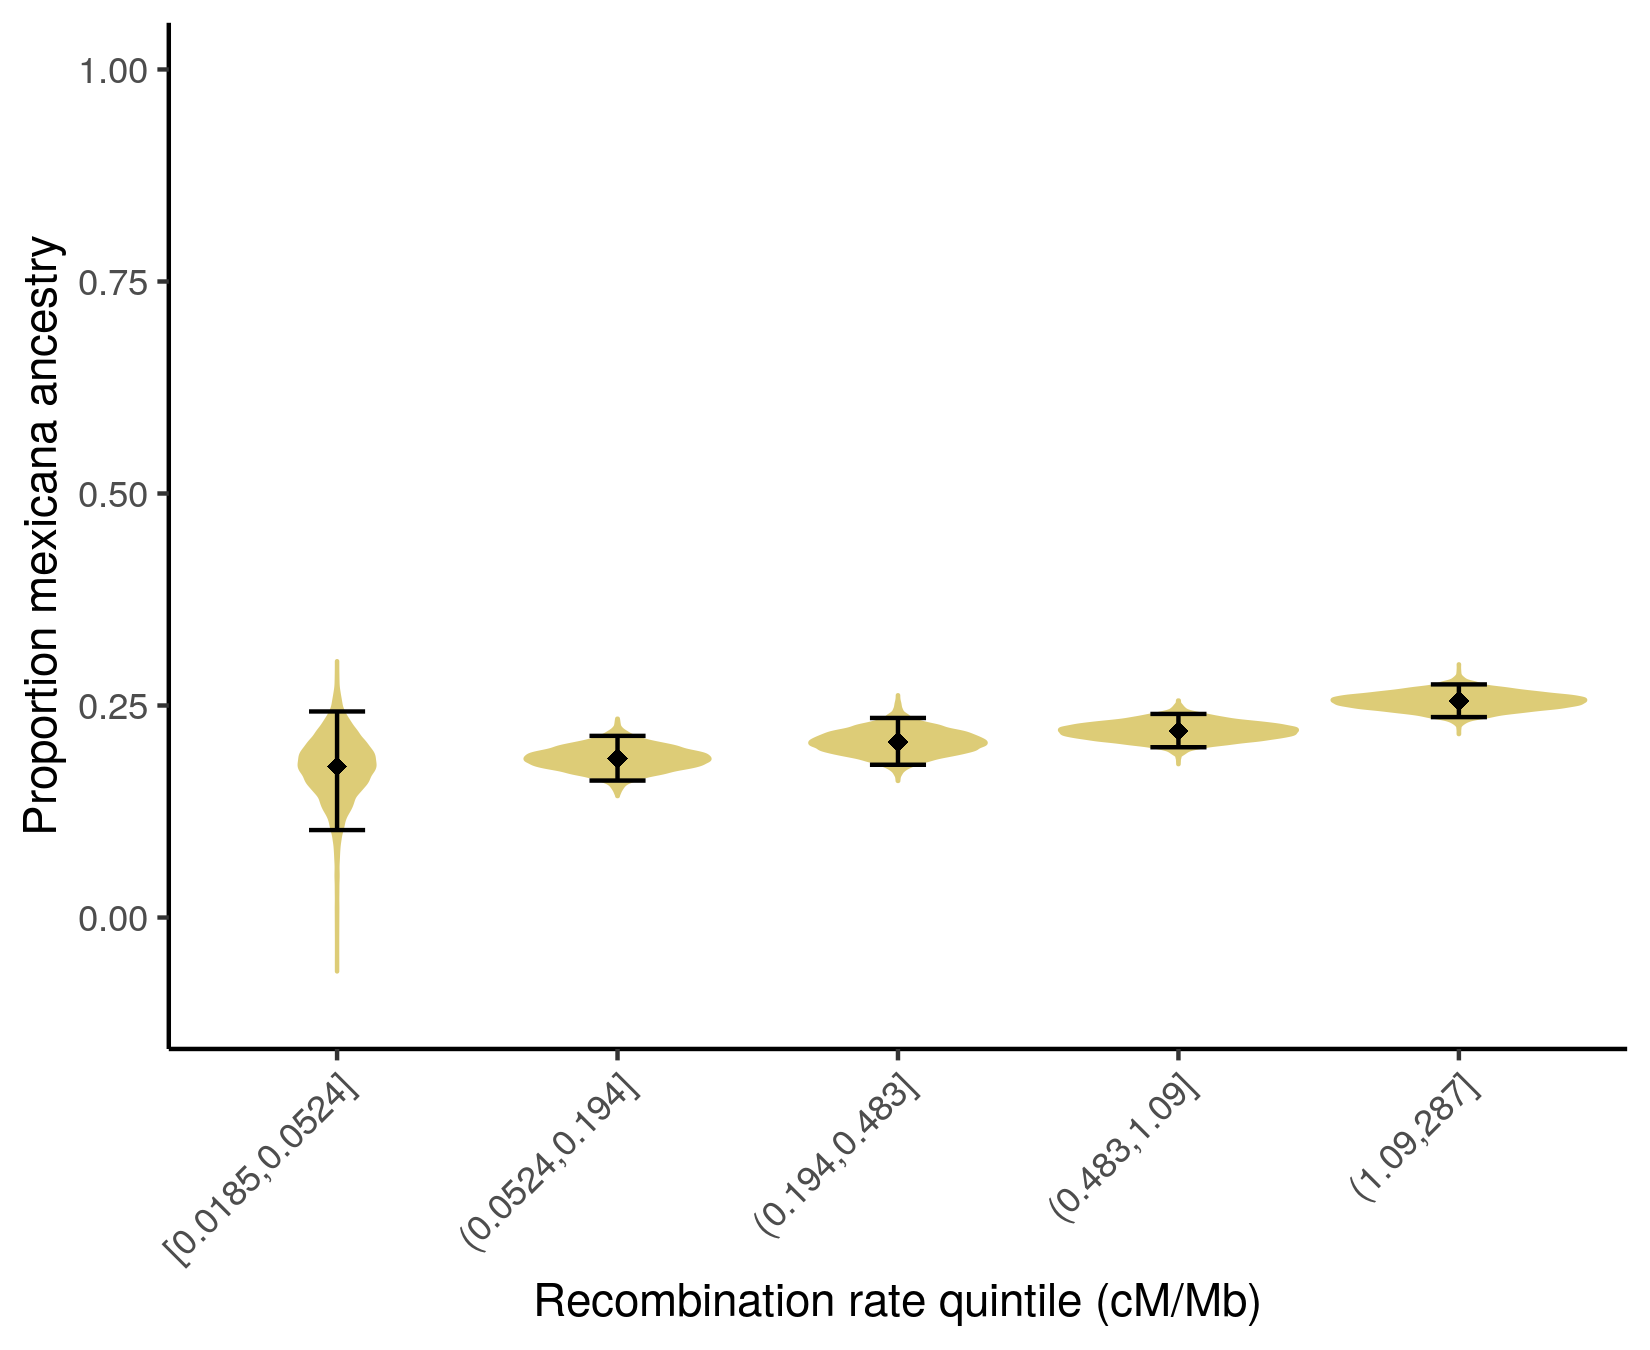
\includegraphics[width=\textwidth]{chapter2/figures/f4_sympatric_maize_pop22_byr5.png}
\caption{\color{Gray} \textbf{$f_4$ ancestry in maize by recombination rate}. Estimated \textit{mexicana} ancestry in sympatric maize landrace samples using $f_4$ ratio. Mean ancestry per recombination rate quintile and 95\% percentile bootstrap confidence interval (n = 10,000) are depicted in black. Violin plots show the density of ancestry estimates for individual bootstraps re-sampled within quintiles.}
\label{f4_maize_by_r}
\end{figure}

%\begin{figure}[p]
\begin{figure}[ht]
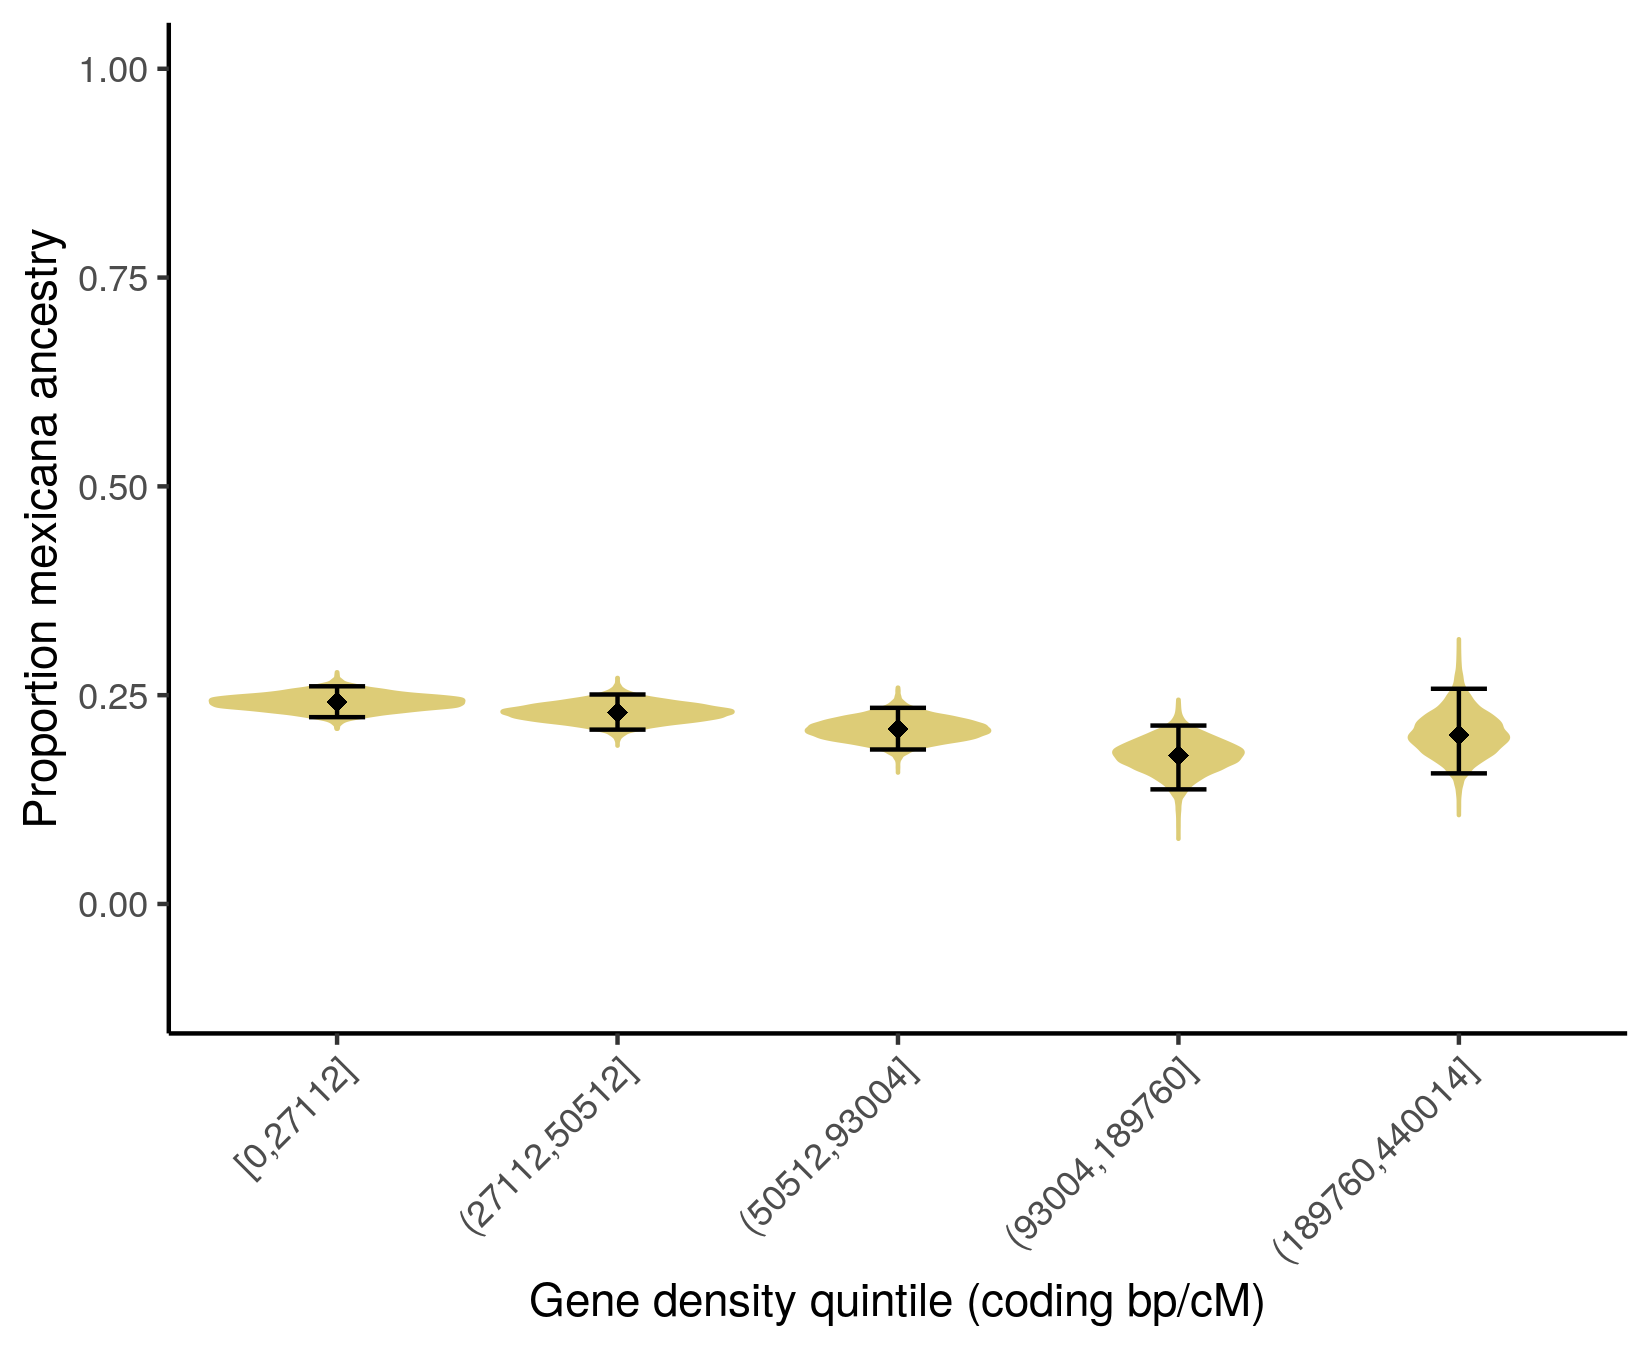
\includegraphics[width=\textwidth]{chapter2/figures/f4_sympatric_maize_pop22_bycd5.png}
\caption{\color{Gray} \textbf{$f_4$ ancestry in maize by coding bp per cM}. Estimated \textit{mexicana} ancestry in sympatric maize landrace samples using $f_4$ ratio. Mean ancestry for each coding bp/cM quintile and 95\% percentile bootstrap confidence interval (n = 10,000) are depicted in black. Violin plots show the density of ancestry estimates for individual bootstraps re-sampled within quintiles.}
\label{f4_maize_by_cd}
\end{figure}

\begin{figure}[ht]
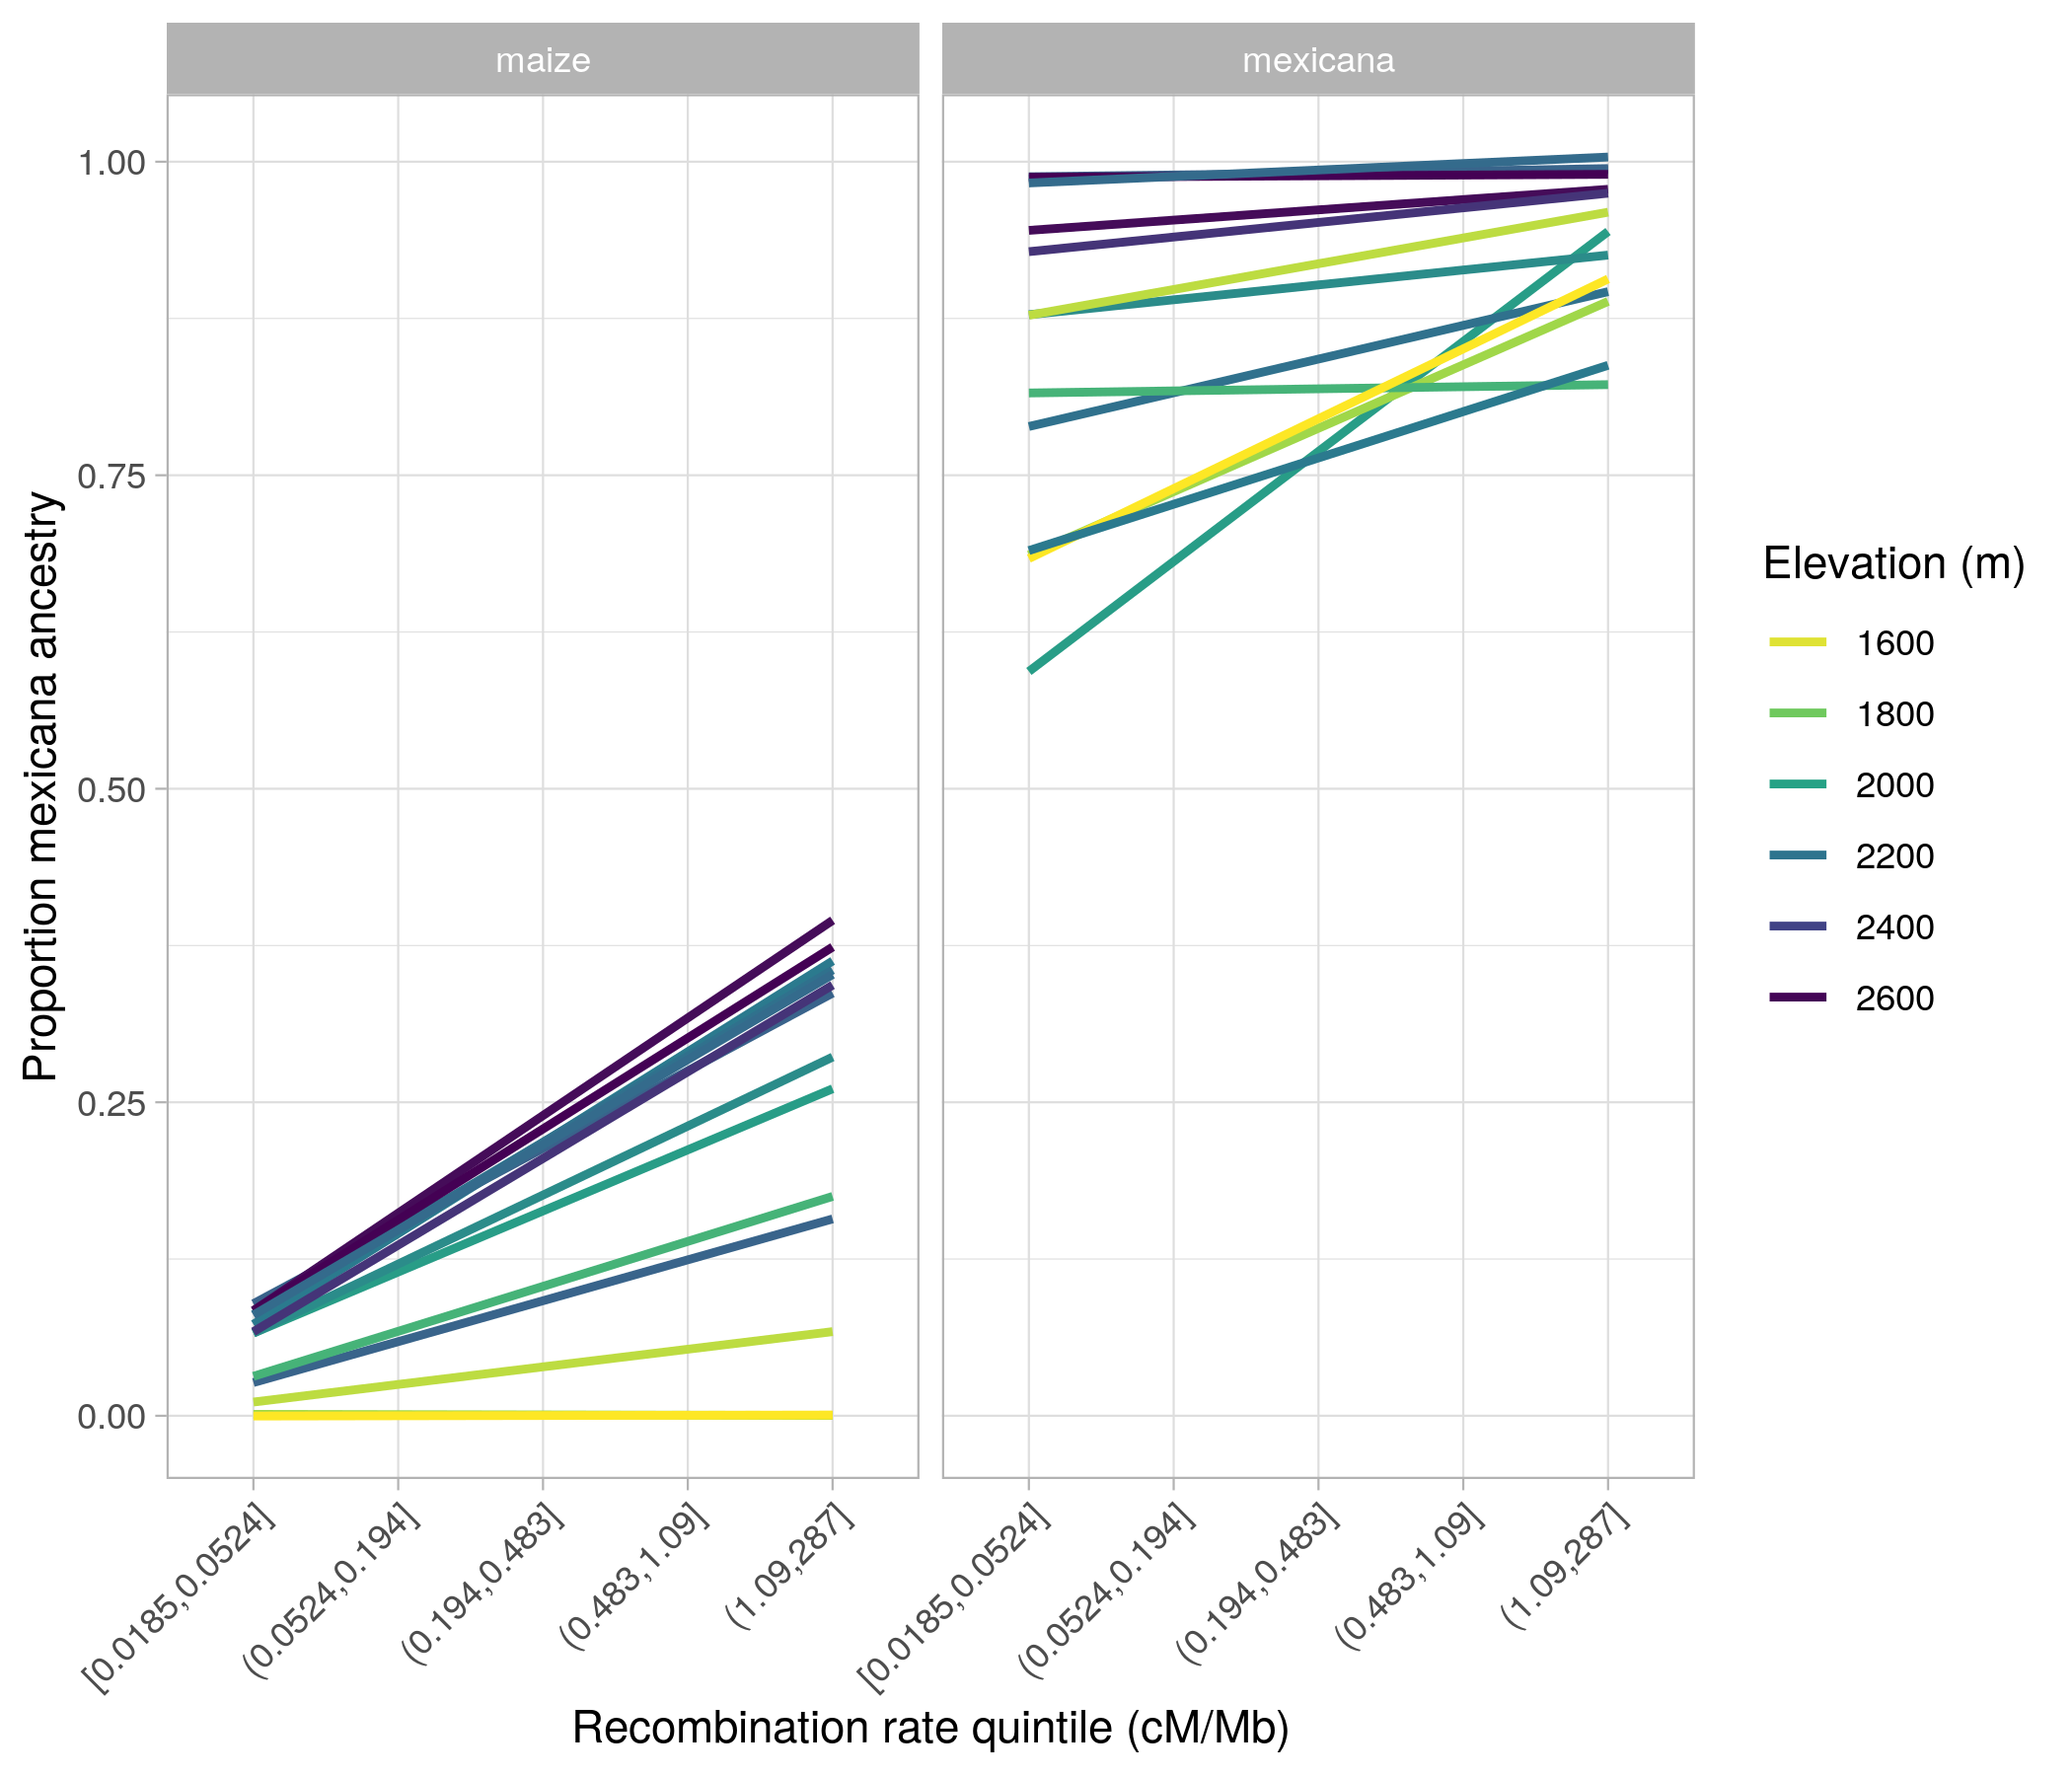
\includegraphics[width=\textwidth]{chapter2/figures/K2_by_r_bootstrap_lm_elevation_color_elev.png}
\caption{\color{Gray} \textbf{\textit{Mexicana} ancestry across recombination quintiles by elevation}. Estimated linear relationship between proportion \mexicana ancestry (NGSAdmix) and recombination rate quintile for each sympatric population, colored by elevation. Linear models were fit using \textit{lm()} in R on individuals' ancestry estimates per quintile.}
\label{K2_by_r_elev_lm}
\end{figure}

%\begin{figure}[p]
\begin{figure}[ht]
\includegraphics[width=\textwidth]{chapter2/figures/K2_by_cd_bootstrap_sympatric_and_allopatric.png}
\caption{\color{Gray} \textbf{\textit{Mexicana} ancestry by coding bp per cM}. Inferred \textit{mexicana} ancestry in  allopatric reference populations (left) and sympatric maize and \textit{mexicana} populations (right) using NGSAdmix (K=2) by coding density quintiles. Group mean and 95\% percentile bootstrap confidence interval (n = 100) are depicted in black. Ancestry estimates for each individual are shown as points, colored by \textit{Zea} subspecies, and points are jittered for better visualization.}
\label{K2_by_cd}
\end{figure}


%\begin{figure}[p]
\begin{figure}[ht]
\includegraphics[width=\textwidth]{chapter2/figures/f4_sympatric_mexicana_pop22_byr5.png}
\caption{\color{Gray} \textbf{$f_4$ ancestry in maize by recombination rate}. Estimated \textit{mexicana} ancestry in sympatric mexicana samples using $f_4$ ratio. Mean ancestry per recombination rate quintile and 95\% percentile bootstrap confidence interval (n = 10,000) are depicted in black. Violin plots show the density of ancestry estimates for individual bootstraps re-sampled within quintiles.}
\label{f4_mexicana_by_r}
\end{figure}

%\begin{figure}[p]
\begin{figure}[ht]
\includegraphics[width=\textwidth]{chapter2/figures/f4_sympatric_mexicana_pop22_bycd5.png}
\caption{\color{Gray} \textbf{$f_4$ ancestry in mexicana by coding bp per cM}. Estimated \textit{mexicana} ancestry in sympatric mexicana samples using $f_4$ ratio. Mean ancestry for each coding bp/cM quintile and 95\% percentile bootstrap confidence interval (n = 10,000) are depicted in black. Violin plots show the density of ancestry estimates for individual bootstraps re-sampled within quintiles.}
\label{f4_mexicana_by_cd}
\end{figure}


%\begin{figure}[p]
\begin{figure}[ht]
\includegraphics[width=\textwidth]{chapter2/figures/local_anc_by_r_continuous.png}
\caption{\color{Gray} \textbf{Local \mexicana ancestry in 1 cM windows by recombination rate}. Estimated \textit{mexicana} ancestry in sympatric maize and \mexicana samples using ancestry\_hmm. Each point is a 1 cM genomic window and the line shows the best linear model fit for mean \mexicana ancestry by recombination rate on a log scale.}
\label{local_ancestry_mexicana_by_log10r}
\end{figure}

\begin{figure}[ht]
\includegraphics[width=\textwidth]{chapter2/figures/combmatrix_peak_sharing_maize.png}
\caption{\color{Gray} \textbf{High introgression peaks shared across sympatric maize populations} Here we show the 75 most common combinations of populations that share ancestry peaks (introgressed ancestry $>$ 2 s.d. above each population's mean ancestry). Bar height represents the percent of SNPs genomewide within peaks shared by the populations highlighted in blue below. Populations are ordered from high (top) to low elevation. See \ref{combmatrix_peaks_mexicana} for sympatric \mexicana equivalent visualization.}
\label{combmatrix_peaks_maize}
\end{figure}

\begin{figure}[ht]
\includegraphics[width=\textwidth]{chapter2/figures/combmatrix_peak_sharing_mexicana.png}
\caption{\color{Gray} \textbf{High introgression peaks shared across sympatric \mexicana populations} Here we show the 75 most common combinations of populations that share ancestry peaks (introgressed ancestry $>$ 2 s.d. above each population's mean ancestry). Bar height represents the percent of SNPs genomewide within peaks shared by the populations highlighted in blue below. Populations are ordered from high (top) to low elevation.}
\label{combmatrix_peaks_mexicana}
\end{figure}

\begin{figure}[ht]
\includegraphics[width=.85\textwidth]{chapter2/figures/maize_shared_outliers_chr_1.png}
\caption{\color{Gray} \textbf{Introgression in maize landrace populations across chromosome 1}}
\label{maize_chr1}
\end{figure}

\begin{figure}[ht]
\includegraphics[width=.85\textwidth]{chapter2/figures/maize_shared_outliers_chr_2.png}
\caption{\color{Gray} \textbf{Introgression in maize landrace populations across chromosome 2}}
\label{maize_chr2}
\end{figure}

\begin{figure}[ht]
\includegraphics[width=.85\textwidth]{chapter2/figures/maize_shared_outliers_chr_3.png}
\caption{\color{Gray} \textbf{Introgression in maize landrace populations across chromosome 3}}
\label{maize_chr3}
\end{figure}

\begin{figure}[ht]
\includegraphics[width=.85\textwidth]{chapter2/figures/maize_shared_outliers_chr_5.png}
\caption{\color{Gray} \textbf{Introgression in maize landrace populations across chromosome 5}}
\label{maize_chr5}
\end{figure}

\begin{figure}[ht]
\includegraphics[width=.85\textwidth]{chapter2/figures/maize_shared_outliers_chr_6.png}
\caption{\color{Gray} \textbf{Introgression in maize landrace populations across chromosome 6}}
\label{maize_chr6}
\end{figure}

\begin{figure}[ht]
\includegraphics[width=.85\textwidth]{chapter2/figures/maize_shared_outliers_chr_7.png}
\caption{\color{Gray} \textbf{Introgression in maize landrace populations across chromosome 7}}
\label{maize_chr7}
\end{figure}

\begin{figure}[ht]
\includegraphics[width=.85\textwidth]{chapter2/figures/maize_shared_outliers_chr_8.png}
\caption{\color{Gray} \textbf{Introgression in maize landrace populations across chromosome 8}}
\label{maize_chr8}
\end{figure}

\begin{figure}[ht]
\includegraphics[width=.85\textwidth]{chapter2/figures/maize_shared_outliers_chr_9.png}
\caption{\color{Gray} \textbf{Introgression in maize landrace populations across chromosome 9}}
\label{maize_chr9}
\end{figure}

\begin{figure}[ht]
\includegraphics[width=.85\textwidth]{chapter2/figures/maize_shared_outliers_chr_10.png}
\caption{\color{Gray} \textbf{Introgression in maize landrace populations across chromosome 10}}
\label{maize_chr10}
\end{figure}

\begin{figure}[ht]
\includegraphics[width=.85\textwidth]{chapter2/figures/mexicana_shared_outliers_chr_1.png}
\caption{\color{Gray} \textbf{Introgression in \mexicana populations across chromosome 1}}
\label{mexicana_chr1}
\end{figure}

\begin{figure}[ht]
\includegraphics[width=.85\textwidth]{chapter2/figures/mexicana_shared_outliers_chr_2.png}
\caption{\color{Gray} \textbf{Introgression in \mexicana populations across chromosome 2}}
\label{mexicana_chr2}
\end{figure}

\begin{figure}[ht]
\includegraphics[width=.85\textwidth]{chapter2/figures/mexicana_shared_outliers_chr_3.png}
\caption{\color{Gray} \textbf{Introgression in \mexicana populations across chromosome 3}}
\label{mexicana_chr3}
\end{figure}

\begin{figure}[ht]
\includegraphics[width=.85\textwidth]{chapter2/figures/mexicana_shared_outliers_chr_4.png}
\caption{\color{Gray} \textbf{Introgression in \mexicana populations across chromosome 4} Vertical lines indicate the coordinates for \textit{Inv4m}.}
\label{mexicana_chr4}
\end{figure}

\begin{figure}[ht]
\includegraphics[width=.85\textwidth]{chapter2/figures/mexicana_shared_outliers_chr_5.png}
\caption{\color{Gray} \textbf{Introgression in \mexicana populations across chromosome 5}}
\label{mexicana_chr5}
\end{figure}

\begin{figure}[ht]
\includegraphics[width=.85\textwidth]{chapter2/figures/mexicana_shared_outliers_chr_6.png}
\caption{\color{Gray} \textbf{Introgression in \mexicana populations across chromosome 6}}
\label{mexicana_chr6}
\end{figure}

\begin{figure}[ht]
\includegraphics[width=.85\textwidth]{chapter2/figures/mexicana_shared_outliers_chr_7.png}
\caption{\color{Gray} \textbf{Introgression in \mexicana populations across chromosome 7}}
\label{mexicana_chr7}
\end{figure}

\begin{figure}[ht]
\includegraphics[width=.85\textwidth]{chapter2/figures/mexicana_shared_outliers_chr_8.png}
\caption{\color{Gray} \textbf{Introgression in \mexicana populations across chromosome 8}}
\label{mexicana_chr8}
\end{figure}

\begin{figure}[ht]
\includegraphics[width=.85\textwidth]{chapter2/figures/mexicana_shared_outliers_chr_9.png}
\caption{\color{Gray} \textbf{Introgression in \mexicana populations across chromosome 9}}
\label{mexicana_chr9}
\end{figure}

\begin{figure}[ht]
\includegraphics[width=.85\textwidth]{chapter2/figures/mexicana_shared_outliers_chr_10.png}
\caption{\color{Gray} \textbf{Introgression in \mexicana populations across chromosome 10}}
\label{mexicana_chr10}
\end{figure}

\begin{figure}[ht]
\includegraphics[width=\textwidth]{chapter2/figures/local_fst_within_mexicana_ancestry_peaks.png}
\caption{\color{Gray} \textbf{Differentiation ($F_{ST}$) between introgressed ancestry tracts and local \mexicana} Each point summarises $F_{ST}$ between \mexicana ancestry tracts within a focal maize population and \mexicana ancestry tracts within the local \mexicana population sampled at the same site. Within-\mexicana ancestry $F_{ST}$ is presented separately for three subsets of the genome: introgression peaks found in the focal maize population only, peaks shared between the focal maize and at least 3 other maize populations, and a genomewide estimate.}
\label{local_fst_peaks}
\end{figure}

\begin{figure}[ht]
\includegraphics[width=\textwidth]{chapter2/figures/QQ.png}
\caption{\color{Gray} \textbf{Quantile comparison of observed data vs. MVN normal null model} (A) QQ-plot of simulated vs. observed mean ancestry at individual loci across all sympatric populations. (B) QQ-plot of simulated vs. observed slopes from the linear model \mexicana ancestry $\sim$ elevation at individual loci.}
\label{QQ}
\end{figure}

%\begin{figure}[p]
\begin{figure}[ht]
\includegraphics[width=\textwidth]{chapter2/figures/mhl1_inv_ancestry.png}
\caption{\color{Gray} \textbf{Ancestry slope with elevation at mhl1 locus}. Slope of introgressed \mexicana ancestry proportion in sympatric maize over a 1 km gain in elevation, zoomed in on the mhl1 QTL region on chromosome 9. Coordinates for the 3 Mb outlier region within this QTL are 9:108640415-111788150.}
\label{mhl1_slopes}
\end{figure}

%\begin{figure}[p]
\begin{figure}[ht]
\includegraphics[width=\textwidth]{chapter2/figures/mhl1_inv_pca.png}
\caption{\color{Gray} \textbf{PCA of putative mhl1 inversion}. Principal components analysis of all SNPs in the 3 Mb outlier region within the mhl1 QTL region that shows a steep increase in introgressed \mexicana ancestry across elevation ($>$5\% FDR). This region on chromosome 9 is a putative inversion (9:108640415-111788150), separating out into three clusters across PC1: individuals homozygous for the common \mexicana inversion allele (left), heterozygous individuals (middle) and individuals homozygous for the common maize inversion allele (right; includes all allopatric maize).}
\label{mhl1_pca}
\end{figure}


  % \appendix

   %\chapter[%
    %  Short Title of Appendix A
  % ]{%
   %   Long Title of Appendix A
  % }%
  % \label{ch:AppendixALabel}
  % \input{AppendixAFileName.tex}
       
   \backmatter
   
   

   
   %This is where your bibliography is generated. Make sure that your .bib file is actually called library.bib
   \bibliography{library}
   
   %This defines the bibliographies style. Search online for a list of available styles.
   \bibliographystyle{plos2015}
   
   
\end{document}